\documentclass[11pt]{article}
\usepackage[margin=1in]{geometry}
\usepackage[T1]{fontenc}
\usepackage{lmodern}
\usepackage{amsmath,amssymb,booktabs,array,graphicx}
\usepackage[round]{natbib}
\usepackage[section]{placeins}
\usepackage[hidelinks]{hyperref}

% Result numbers. Generated by `crew.py numbers`; never typed by hand.
% Generated by `crew.py numbers` from claims.jsonl. Do not edit by hand.
% Each macro is a number taken from a logged run; see claims.jsonl.
\newcommand{\NCells}{600}  % c-n-cells
\newcommand{\NFlipFail}{0}  % c-flip-fail
\newcommand{\NConvWarnCells}{0}  % c-convwarn
\newcommand{\MajBc}{0.632}  % c-m-Bc
\newcommand{\AccBcLrZero}{0.970}  % c-acc-Bc-Lr-Zero
\newcommand{\SdBcLrZero}{0.010}  % c-sd-Bc-Lr-Zero
\newcommand{\PmsBcLrZero}{0.651}  % c-pms-Bc-Lr-Zero
\newcommand{\VnBcLrZero}{0.975}  % c-vn-Bc-Lr-Zero
\newcommand{\VcBcLrZero}{0.975}  % c-vc-Bc-Lr-Zero
\newcommand{\TnBcLrZero}{0.987}  % c-tn-Bc-Lr-Zero
\newcommand{\CBcZero}{0.276}  % c-C-Bc-Zero
\newcommand{\AccBcLrOne}{0.954}  % c-acc-Bc-Lr-One
\newcommand{\SdBcLrOne}{0.029}  % c-sd-Bc-Lr-One
\newcommand{\PmsBcLrOne}{0.665}  % c-pms-Bc-Lr-One
\newcommand{\VnBcLrOne}{0.875}  % c-vn-Bc-Lr-One
\newcommand{\VcBcLrOne}{0.954}  % c-vc-Bc-Lr-One
\newcommand{\TnBcLrOne}{0.875}  % c-tn-Bc-Lr-One
\newcommand{\CBcOne}{0.104}  % c-C-Bc-One
\newcommand{\AccBcLrTwo}{0.949}  % c-acc-Bc-Lr-Two
\newcommand{\SdBcLrTwo}{0.020}  % c-sd-Bc-Lr-Two
\newcommand{\PmsBcLrTwo}{0.667}  % c-pms-Bc-Lr-Two
\newcommand{\VnBcLrTwo}{0.777}  % c-vn-Bc-Lr-Two
\newcommand{\VcBcLrTwo}{0.953}  % c-vc-Bc-Lr-Two
\newcommand{\TnBcLrTwo}{0.777}  % c-tn-Bc-Lr-Two
\newcommand{\CBcTwo}{0.0492}  % c-C-Bc-Two
\newcommand{\AccBcLrThree}{0.907}  % c-acc-Bc-Lr-Three
\newcommand{\SdBcLrThree}{0.027}  % c-sd-Bc-Lr-Three
\newcommand{\PmsBcLrThree}{0.672}  % c-pms-Bc-Lr-Three
\newcommand{\VnBcLrThree}{0.689}  % c-vn-Bc-Lr-Three
\newcommand{\VcBcLrThree}{0.909}  % c-vc-Bc-Lr-Three
\newcommand{\TnBcLrThree}{0.684}  % c-tn-Bc-Lr-Three
\newcommand{\CBcThree}{0.051}  % c-C-Bc-Three
\newcommand{\AccBcLrFour}{0.781}  % c-acc-Bc-Lr-Four
\newcommand{\SdBcLrFour}{0.098}  % c-sd-Bc-Lr-Four
\newcommand{\PmsBcLrFour}{0.670}  % c-pms-Bc-Lr-Four
\newcommand{\VnBcLrFour}{0.597}  % c-vn-Bc-Lr-Four
\newcommand{\VcBcLrFour}{0.764}  % c-vc-Bc-Lr-Four
\newcommand{\TnBcLrFour}{0.593}  % c-tn-Bc-Lr-Four
\newcommand{\CBcFour}{0.0428}  % c-C-Bc-Four
\newcommand{\AccBcRfZero}{0.951}  % c-acc-Bc-Rf-Zero
\newcommand{\SdBcRfZero}{0.032}  % c-sd-Bc-Rf-Zero
\newcommand{\PmsBcRfZero}{0.633}  % c-pms-Bc-Rf-Zero
\newcommand{\VnBcRfZero}{0.961}  % c-vn-Bc-Rf-Zero
\newcommand{\VcBcRfZero}{0.961}  % c-vc-Bc-Rf-Zero
\newcommand{\TnBcRfZero}{0.988}  % c-tn-Bc-Rf-Zero
\newcommand{\MslBcZero}{2.5}  % c-msl-Bc-Zero
\newcommand{\MfBcZero}{0.24}  % c-mf-Bc-Zero
\newcommand{\AccBcRfOne}{0.948}  % c-acc-Bc-Rf-One
\newcommand{\SdBcRfOne}{0.027}  % c-sd-Bc-Rf-One
\newcommand{\PmsBcRfOne}{0.632}  % c-pms-Bc-Rf-One
\newcommand{\VnBcRfOne}{0.877}  % c-vn-Bc-Rf-One
\newcommand{\VcBcRfOne}{0.958}  % c-vc-Bc-Rf-One
\newcommand{\TnBcRfOne}{0.921}  % c-tn-Bc-Rf-One
\newcommand{\MslBcOne}{3}  % c-msl-Bc-One
\newcommand{\MfBcOne}{0.40}  % c-mf-Bc-One
\newcommand{\AccBcRfTwo}{0.943}  % c-acc-Bc-Rf-Two
\newcommand{\SdBcRfTwo}{0.033}  % c-sd-Bc-Rf-Two
\newcommand{\PmsBcRfTwo}{0.627}  % c-pms-Bc-Rf-Two
\newcommand{\VnBcRfTwo}{0.792}  % c-vn-Bc-Rf-Two
\newcommand{\VcBcRfTwo}{0.954}  % c-vc-Bc-Rf-Two
\newcommand{\TnBcRfTwo}{0.876}  % c-tn-Bc-Rf-Two
\newcommand{\MslBcTwo}{6.5}  % c-msl-Bc-Two
\newcommand{\MfBcTwo}{0.20}  % c-mf-Bc-Two
\newcommand{\AccBcRfThree}{0.922}  % c-acc-Bc-Rf-Three
\newcommand{\SdBcRfThree}{0.026}  % c-sd-Bc-Rf-Three
\newcommand{\PmsBcRfThree}{0.636}  % c-pms-Bc-Rf-Three
\newcommand{\VnBcRfThree}{0.704}  % c-vn-Bc-Rf-Three
\newcommand{\VcBcRfThree}{0.923}  % c-vc-Bc-Rf-Three
\newcommand{\TnBcRfThree}{0.764}  % c-tn-Bc-Rf-Three
\newcommand{\MslBcThree}{15}  % c-msl-Bc-Three
\newcommand{\MfBcThree}{0.49}  % c-mf-Bc-Three
\newcommand{\AccBcRfFour}{0.846}  % c-acc-Bc-Rf-Four
\newcommand{\SdBcRfFour}{0.074}  % c-sd-Bc-Rf-Four
\newcommand{\PmsBcRfFour}{0.581}  % c-pms-Bc-Rf-Four
\newcommand{\VnBcRfFour}{0.596}  % c-vn-Bc-Rf-Four
\newcommand{\VcBcRfFour}{0.834}  % c-vc-Bc-Rf-Four
\newcommand{\TnBcRfFour}{0.755}  % c-tn-Bc-Rf-Four
\newcommand{\MslBcFour}{19.5}  % c-msl-Bc-Four
\newcommand{\MfBcFour}{0.38}  % c-mf-Bc-Four
\newcommand{\AccBcGbZero}{0.954}  % c-acc-Bc-Gb-Zero
\newcommand{\SdBcGbZero}{0.031}  % c-sd-Bc-Gb-Zero
\newcommand{\PmsBcGbZero}{0.632}  % c-pms-Bc-Gb-Zero
\newcommand{\VnBcGbZero}{0.975}  % c-vn-Bc-Gb-Zero
\newcommand{\VcBcGbZero}{0.975}  % c-vc-Bc-Gb-Zero
\newcommand{\TnBcGbZero}{1.000}  % c-tn-Bc-Gb-Zero
\newcommand{\LrateBcZero}{0.057}  % c-lrate-Bc-Zero
\newcommand{\IterBcZero}{167}  % c-iter-Bc-Zero
\newcommand{\AccBcGbOne}{0.942}  % c-acc-Bc-Gb-One
\newcommand{\SdBcGbOne}{0.033}  % c-sd-Bc-Gb-One
\newcommand{\PmsBcGbOne}{0.625}  % c-pms-Bc-Gb-One
\newcommand{\VnBcGbOne}{0.882}  % c-vn-Bc-Gb-One
\newcommand{\VcBcGbOne}{0.958}  % c-vc-Bc-Gb-One
\newcommand{\TnBcGbOne}{0.964}  % c-tn-Bc-Gb-One
\newcommand{\LrateBcOne}{0.0728}  % c-lrate-Bc-One
\newcommand{\IterBcOne}{62}  % c-iter-Bc-One
\newcommand{\AccBcGbTwo}{0.927}  % c-acc-Bc-Gb-Two
\newcommand{\SdBcGbTwo}{0.044}  % c-sd-Bc-Gb-Two
\newcommand{\PmsBcGbTwo}{0.625}  % c-pms-Bc-Gb-Two
\newcommand{\VnBcGbTwo}{0.782}  % c-vn-Bc-Gb-Two
\newcommand{\VcBcGbTwo}{0.939}  % c-vc-Bc-Gb-Two
\newcommand{\TnBcGbTwo}{0.889}  % c-tn-Bc-Gb-Two
\newcommand{\LrateBcTwo}{0.0743}  % c-lrate-Bc-Two
\newcommand{\IterBcTwo}{54}  % c-iter-Bc-Two
\newcommand{\AccBcGbThree}{0.911}  % c-acc-Bc-Gb-Three
\newcommand{\SdBcGbThree}{0.045}  % c-sd-Bc-Gb-Three
\newcommand{\PmsBcGbThree}{0.629}  % c-pms-Bc-Gb-Three
\newcommand{\VnBcGbThree}{0.698}  % c-vn-Bc-Gb-Three
\newcommand{\VcBcGbThree}{0.918}  % c-vc-Bc-Gb-Three
\newcommand{\TnBcGbThree}{0.752}  % c-tn-Bc-Gb-Three
\newcommand{\LrateBcThree}{0.0233}  % c-lrate-Bc-Three
\newcommand{\IterBcThree}{82}  % c-iter-Bc-Three
\newcommand{\AccBcGbFour}{0.762}  % c-acc-Bc-Gb-Four
\newcommand{\SdBcGbFour}{0.079}  % c-sd-Bc-Gb-Four
\newcommand{\PmsBcGbFour}{0.568}  % c-pms-Bc-Gb-Four
\newcommand{\VnBcGbFour}{0.604}  % c-vn-Bc-Gb-Four
\newcommand{\VcBcGbFour}{0.756}  % c-vc-Bc-Gb-Four
\newcommand{\TnBcGbFour}{0.800}  % c-tn-Bc-Gb-Four
\newcommand{\LrateBcFour}{0.0717}  % c-lrate-Bc-Four
\newcommand{\IterBcFour}{31}  % c-iter-Bc-Four
\newcommand{\MajCg}{0.700}  % c-m-Cg
\newcommand{\AccCgLrZero}{0.750}  % c-acc-Cg-Lr-Zero
\newcommand{\SdCgLrZero}{0.018}  % c-sd-Cg-Lr-Zero
\newcommand{\PmsCgLrZero}{0.795}  % c-pms-Cg-Lr-Zero
\newcommand{\VnCgLrZero}{0.762}  % c-vn-Cg-Lr-Zero
\newcommand{\VcCgLrZero}{0.762}  % c-vc-Cg-Lr-Zero
\newcommand{\TnCgLrZero}{0.788}  % c-tn-Cg-Lr-Zero
\newcommand{\CCgZero}{0.272}  % c-C-Cg-Zero
\newcommand{\AccCgLrOne}{0.741}  % c-acc-Cg-Lr-One
\newcommand{\SdCgLrOne}{0.016}  % c-sd-Cg-Lr-One
\newcommand{\PmsCgLrOne}{0.793}  % c-pms-Cg-Lr-One
\newcommand{\VnCgLrOne}{0.718}  % c-vn-Cg-Lr-One
\newcommand{\VcCgLrOne}{0.758}  % c-vc-Cg-Lr-One
\newcommand{\TnCgLrOne}{0.739}  % c-tn-Cg-Lr-One
\newcommand{\CCgOne}{0.255}  % c-C-Cg-One
\newcommand{\AccCgLrTwo}{0.715}  % c-acc-Cg-Lr-Two
\newcommand{\SdCgLrTwo}{0.019}  % c-sd-Cg-Lr-Two
\newcommand{\PmsCgLrTwo}{0.839}  % c-pms-Cg-Lr-Two
\newcommand{\VnCgLrTwo}{0.666}  % c-vn-Cg-Lr-Two
\newcommand{\VcCgLrTwo}{0.734}  % c-vc-Cg-Lr-Two
\newcommand{\TnCgLrTwo}{0.677}  % c-tn-Cg-Lr-Two
\newcommand{\CCgTwo}{0.0654}  % c-C-Cg-Two
\newcommand{\AccCgLrThree}{0.710}  % c-acc-Cg-Lr-Three
\newcommand{\SdCgLrThree}{0.028}  % c-sd-Cg-Lr-Three
\newcommand{\PmsCgLrThree}{0.839}  % c-pms-Cg-Lr-Three
\newcommand{\VnCgLrThree}{0.611}  % c-vn-Cg-Lr-Three
\newcommand{\VcCgLrThree}{0.718}  % c-vc-Cg-Lr-Three
\newcommand{\TnCgLrThree}{0.635}  % c-tn-Cg-Lr-Three
\newcommand{\CCgThree}{0.0336}  % c-C-Cg-Three
\newcommand{\AccCgLrFour}{0.674}  % c-acc-Cg-Lr-Four
\newcommand{\SdCgLrFour}{0.053}  % c-sd-Cg-Lr-Four
\newcommand{\PmsCgLrFour}{0.867}  % c-pms-Cg-Lr-Four
\newcommand{\VnCgLrFour}{0.576}  % c-vn-Cg-Lr-Four
\newcommand{\VcCgLrFour}{0.683}  % c-vc-Cg-Lr-Four
\newcommand{\TnCgLrFour}{0.572}  % c-tn-Cg-Lr-Four
\newcommand{\CCgFour}{0.00698}  % c-C-Cg-Four
\newcommand{\AccCgRfZero}{0.749}  % c-acc-Cg-Rf-Zero
\newcommand{\SdCgRfZero}{0.020}  % c-sd-Cg-Rf-Zero
\newcommand{\PmsCgRfZero}{0.823}  % c-pms-Cg-Rf-Zero
\newcommand{\VnCgRfZero}{0.781}  % c-vn-Cg-Rf-Zero
\newcommand{\VcCgRfZero}{0.781}  % c-vc-Cg-Rf-Zero
\newcommand{\TnCgRfZero}{0.929}  % c-tn-Cg-Rf-Zero
\newcommand{\MslCgZero}{2}  % c-msl-Cg-Zero
\newcommand{\MfCgZero}{0.26}  % c-mf-Cg-Zero
\newcommand{\AccCgRfOne}{0.739}  % c-acc-Cg-Rf-One
\newcommand{\SdCgRfOne}{0.019}  % c-sd-Cg-Rf-One
\newcommand{\PmsCgRfOne}{0.828}  % c-pms-Cg-Rf-One
\newcommand{\VnCgRfOne}{0.725}  % c-vn-Cg-Rf-One
\newcommand{\VcCgRfOne}{0.767}  % c-vc-Cg-Rf-One
\newcommand{\TnCgRfOne}{0.882}  % c-tn-Cg-Rf-One
\newcommand{\MslCgOne}{5.5}  % c-msl-Cg-One
\newcommand{\MfCgOne}{0.29}  % c-mf-Cg-One
\newcommand{\AccCgRfTwo}{0.731}  % c-acc-Cg-Rf-Two
\newcommand{\SdCgRfTwo}{0.017}  % c-sd-Cg-Rf-Two
\newcommand{\PmsCgRfTwo}{0.815}  % c-pms-Cg-Rf-Two
\newcommand{\VnCgRfTwo}{0.681}  % c-vn-Cg-Rf-Two
\newcommand{\VcCgRfTwo}{0.753}  % c-vc-Cg-Rf-Two
\newcommand{\TnCgRfTwo}{0.853}  % c-tn-Cg-Rf-Two
\newcommand{\MslCgTwo}{4.5}  % c-msl-Cg-Two
\newcommand{\MfCgTwo}{0.28}  % c-mf-Cg-Two
\newcommand{\AccCgRfThree}{0.703}  % c-acc-Cg-Rf-Three
\newcommand{\SdCgRfThree}{0.031}  % c-sd-Cg-Rf-Three
\newcommand{\PmsCgRfThree}{0.843}  % c-pms-Cg-Rf-Three
\newcommand{\VnCgRfThree}{0.629}  % c-vn-Cg-Rf-Three
\newcommand{\VcCgRfThree}{0.725}  % c-vc-Cg-Rf-Three
\newcommand{\TnCgRfThree}{0.773}  % c-tn-Cg-Rf-Three
\newcommand{\MslCgThree}{9}  % c-msl-Cg-Three
\newcommand{\MfCgThree}{0.30}  % c-mf-Cg-Three
\newcommand{\AccCgRfFour}{0.638}  % c-acc-Cg-Rf-Four
\newcommand{\SdCgRfFour}{0.047}  % c-sd-Cg-Rf-Four
\newcommand{\PmsCgRfFour}{0.728}  % c-pms-Cg-Rf-Four
\newcommand{\VnCgRfFour}{0.585}  % c-vn-Cg-Rf-Four
\newcommand{\VcCgRfFour}{0.661}  % c-vc-Cg-Rf-Four
\newcommand{\TnCgRfFour}{0.732}  % c-tn-Cg-Rf-Four
\newcommand{\MslCgFour}{15.5}  % c-msl-Cg-Four
\newcommand{\MfCgFour}{0.32}  % c-mf-Cg-Four
\newcommand{\AccCgGbZero}{0.735}  % c-acc-Cg-Gb-Zero
\newcommand{\SdCgGbZero}{0.016}  % c-sd-Cg-Gb-Zero
\newcommand{\PmsCgGbZero}{0.791}  % c-pms-Cg-Gb-Zero
\newcommand{\VnCgGbZero}{0.783}  % c-vn-Cg-Gb-Zero
\newcommand{\VcCgGbZero}{0.783}  % c-vc-Cg-Gb-Zero
\newcommand{\TnCgGbZero}{0.932}  % c-tn-Cg-Gb-Zero
\newcommand{\LrateCgZero}{0.158}  % c-lrate-Cg-Zero
\newcommand{\IterCgZero}{56}  % c-iter-Cg-Zero
\newcommand{\AccCgGbOne}{0.729}  % c-acc-Cg-Gb-One
\newcommand{\SdCgGbOne}{0.026}  % c-sd-Cg-Gb-One
\newcommand{\PmsCgGbOne}{0.779}  % c-pms-Cg-Gb-One
\newcommand{\VnCgGbOne}{0.730}  % c-vn-Cg-Gb-One
\newcommand{\VcCgGbOne}{0.764}  % c-vc-Cg-Gb-One
\newcommand{\TnCgGbOne}{0.856}  % c-tn-Cg-Gb-One
\newcommand{\LrateCgOne}{0.044}  % c-lrate-Cg-One
\newcommand{\IterCgOne}{76}  % c-iter-Cg-One
\newcommand{\AccCgGbTwo}{0.714}  % c-acc-Cg-Gb-Two
\newcommand{\SdCgGbTwo}{0.018}  % c-sd-Cg-Gb-Two
\newcommand{\PmsCgGbTwo}{0.797}  % c-pms-Cg-Gb-Two
\newcommand{\VnCgGbTwo}{0.684}  % c-vn-Cg-Gb-Two
\newcommand{\VcCgGbTwo}{0.742}  % c-vc-Cg-Gb-Two
\newcommand{\TnCgGbTwo}{0.793}  % c-tn-Cg-Gb-Two
\newcommand{\LrateCgTwo}{0.0254}  % c-lrate-Cg-Two
\newcommand{\IterCgTwo}{102}  % c-iter-Cg-Two
\newcommand{\AccCgGbThree}{0.692}  % c-acc-Cg-Gb-Three
\newcommand{\SdCgGbThree}{0.027}  % c-sd-Cg-Gb-Three
\newcommand{\PmsCgGbThree}{0.793}  % c-pms-Cg-Gb-Three
\newcommand{\VnCgGbThree}{0.626}  % c-vn-Cg-Gb-Three
\newcommand{\VcCgGbThree}{0.705}  % c-vc-Cg-Gb-Three
\newcommand{\TnCgGbThree}{0.728}  % c-tn-Cg-Gb-Three
\newcommand{\LrateCgThree}{0.0316}  % c-lrate-Cg-Three
\newcommand{\IterCgThree}{53}  % c-iter-Cg-Three
\newcommand{\AccCgGbFour}{0.647}  % c-acc-Cg-Gb-Four
\newcommand{\SdCgGbFour}{0.046}  % c-sd-Cg-Gb-Four
\newcommand{\PmsCgGbFour}{0.783}  % c-pms-Cg-Gb-Four
\newcommand{\VnCgGbFour}{0.581}  % c-vn-Cg-Gb-Four
\newcommand{\VcCgGbFour}{0.651}  % c-vc-Cg-Gb-Four
\newcommand{\TnCgGbFour}{0.667}  % c-tn-Cg-Gb-Four
\newcommand{\LrateCgFour}{0.0251}  % c-lrate-Cg-Four
\newcommand{\IterCgFour}{29}  % c-iter-Cg-Four
\newcommand{\MajAd}{0.761}  % c-m-Ad
\newcommand{\AccAdLrZero}{0.843}  % c-acc-Ad-Lr-Zero
\newcommand{\SdAdLrZero}{0.012}  % c-sd-Ad-Lr-Zero
\newcommand{\PmsAdLrZero}{0.812}  % c-pms-Ad-Lr-Zero
\newcommand{\VnAdLrZero}{0.849}  % c-vn-Ad-Lr-Zero
\newcommand{\VcAdLrZero}{0.849}  % c-vc-Ad-Lr-Zero
\newcommand{\TnAdLrZero}{0.855}  % c-tn-Ad-Lr-Zero
\newcommand{\CAdZero}{0.38}  % c-C-Ad-Zero
\newcommand{\AccAdLrOne}{0.838}  % c-acc-Ad-Lr-One
\newcommand{\SdAdLrOne}{0.010}  % c-sd-Ad-Lr-One
\newcommand{\PmsAdLrOne}{0.822}  % c-pms-Ad-Lr-One
\newcommand{\VnAdLrOne}{0.776}  % c-vn-Ad-Lr-One
\newcommand{\VcAdLrOne}{0.844}  % c-vc-Ad-Lr-One
\newcommand{\TnAdLrOne}{0.780}  % c-tn-Ad-Lr-One
\newcommand{\CAdOne}{0.182}  % c-C-Ad-One
\newcommand{\AccAdLrTwo}{0.830}  % c-acc-Ad-Lr-Two
\newcommand{\SdAdLrTwo}{0.009}  % c-sd-Ad-Lr-Two
\newcommand{\PmsAdLrTwo}{0.848}  % c-pms-Ad-Lr-Two
\newcommand{\VnAdLrTwo}{0.703}  % c-vn-Ad-Lr-Two
\newcommand{\VcAdLrTwo}{0.833}  % c-vc-Ad-Lr-Two
\newcommand{\TnAdLrTwo}{0.703}  % c-tn-Ad-Lr-Two
\newcommand{\CAdTwo}{0.0195}  % c-C-Ad-Two
\newcommand{\AccAdLrThree}{0.821}  % c-acc-Ad-Lr-Three
\newcommand{\SdAdLrThree}{0.009}  % c-sd-Ad-Lr-Three
\newcommand{\PmsAdLrThree}{0.847}  % c-pms-Ad-Lr-Three
\newcommand{\VnAdLrThree}{0.637}  % c-vn-Ad-Lr-Three
\newcommand{\VcAdLrThree}{0.823}  % c-vc-Ad-Lr-Three
\newcommand{\TnAdLrThree}{0.637}  % c-tn-Ad-Lr-Three
\newcommand{\CAdThree}{0.0202}  % c-C-Ad-Three
\newcommand{\AccAdLrFour}{0.797}  % c-acc-Ad-Lr-Four
\newcommand{\SdAdLrFour}{0.015}  % c-sd-Ad-Lr-Four
\newcommand{\PmsAdLrFour}{0.833}  % c-pms-Ad-Lr-Four
\newcommand{\VnAdLrFour}{0.569}  % c-vn-Ad-Lr-Four
\newcommand{\VcAdLrFour}{0.804}  % c-vc-Ad-Lr-Four
\newcommand{\TnAdLrFour}{0.572}  % c-tn-Ad-Lr-Four
\newcommand{\CAdFour}{0.00584}  % c-C-Ad-Four
\newcommand{\AccAdRfZero}{0.847}  % c-acc-Ad-Rf-Zero
\newcommand{\SdAdRfZero}{0.010}  % c-sd-Ad-Rf-Zero
\newcommand{\PmsAdRfZero}{0.814}  % c-pms-Ad-Rf-Zero
\newcommand{\VnAdRfZero}{0.859}  % c-vn-Ad-Rf-Zero
\newcommand{\VcAdRfZero}{0.859}  % c-vc-Ad-Rf-Zero
\newcommand{\TnAdRfZero}{0.911}  % c-tn-Ad-Rf-Zero
\newcommand{\MslAdZero}{3}  % c-msl-Ad-Zero
\newcommand{\MfAdZero}{0.20}  % c-mf-Ad-Zero
\newcommand{\AccAdRfOne}{0.845}  % c-acc-Ad-Rf-One
\newcommand{\SdAdRfOne}{0.012}  % c-sd-Ad-Rf-One
\newcommand{\PmsAdRfOne}{0.812}  % c-pms-Ad-Rf-One
\newcommand{\VnAdRfOne}{0.788}  % c-vn-Ad-Rf-One
\newcommand{\VcAdRfOne}{0.855}  % c-vc-Ad-Rf-One
\newcommand{\TnAdRfOne}{0.829}  % c-tn-Ad-Rf-One
\newcommand{\MslAdOne}{3.5}  % c-msl-Ad-One
\newcommand{\MfAdOne}{0.22}  % c-mf-Ad-One
\newcommand{\AccAdRfTwo}{0.836}  % c-acc-Ad-Rf-Two
\newcommand{\SdAdRfTwo}{0.006}  % c-sd-Ad-Rf-Two
\newcommand{\PmsAdRfTwo}{0.823}  % c-pms-Ad-Rf-Two
\newcommand{\VnAdRfTwo}{0.714}  % c-vn-Ad-Rf-Two
\newcommand{\VcAdRfTwo}{0.847}  % c-vc-Ad-Rf-Two
\newcommand{\TnAdRfTwo}{0.760}  % c-tn-Ad-Rf-Two
\newcommand{\MslAdTwo}{2.5}  % c-msl-Ad-Two
\newcommand{\MfAdTwo}{0.11}  % c-mf-Ad-Two
\newcommand{\AccAdRfThree}{0.830}  % c-acc-Ad-Rf-Three
\newcommand{\SdAdRfThree}{0.016}  % c-sd-Ad-Rf-Three
\newcommand{\PmsAdRfThree}{0.809}  % c-pms-Ad-Rf-Three
\newcommand{\VnAdRfThree}{0.644}  % c-vn-Ad-Rf-Three
\newcommand{\VcAdRfThree}{0.834}  % c-vc-Ad-Rf-Three
\newcommand{\TnAdRfThree}{0.715}  % c-tn-Ad-Rf-Three
\newcommand{\MslAdThree}{11}  % c-msl-Ad-Three
\newcommand{\MfAdThree}{0.13}  % c-mf-Ad-Three
\newcommand{\AccAdRfFour}{0.794}  % c-acc-Ad-Rf-Four
\newcommand{\SdAdRfFour}{0.021}  % c-sd-Ad-Rf-Four
\newcommand{\PmsAdRfFour}{0.776}  % c-pms-Ad-Rf-Four
\newcommand{\VnAdRfFour}{0.571}  % c-vn-Ad-Rf-Four
\newcommand{\VcAdRfFour}{0.804}  % c-vc-Ad-Rf-Four
\newcommand{\TnAdRfFour}{0.646}  % c-tn-Ad-Rf-Four
\newcommand{\MslAdFour}{23}  % c-msl-Ad-Four
\newcommand{\MfAdFour}{0.28}  % c-mf-Ad-Four
\newcommand{\AccAdGbZero}{0.852}  % c-acc-Ad-Gb-Zero
\newcommand{\SdAdGbZero}{0.009}  % c-sd-Ad-Gb-Zero
\newcommand{\PmsAdGbZero}{0.803}  % c-pms-Ad-Gb-Zero
\newcommand{\VnAdGbZero}{0.866}  % c-vn-Ad-Gb-Zero
\newcommand{\VcAdGbZero}{0.866}  % c-vc-Ad-Gb-Zero
\newcommand{\TnAdGbZero}{0.907}  % c-tn-Ad-Gb-Zero
\newcommand{\LrateAdZero}{0.109}  % c-lrate-Ad-Zero
\newcommand{\IterAdZero}{94}  % c-iter-Ad-Zero
\newcommand{\AccAdGbOne}{0.850}  % c-acc-Ad-Gb-One
\newcommand{\SdAdGbOne}{0.007}  % c-sd-Ad-Gb-One
\newcommand{\PmsAdGbOne}{0.821}  % c-pms-Ad-Gb-One
\newcommand{\VnAdGbOne}{0.792}  % c-vn-Ad-Gb-One
\newcommand{\VcAdGbOne}{0.861}  % c-vc-Ad-Gb-One
\newcommand{\TnAdGbOne}{0.813}  % c-tn-Ad-Gb-One
\newcommand{\LrateAdOne}{0.0201}  % c-lrate-Ad-One
\newcommand{\IterAdOne}{173}  % c-iter-Ad-One
\newcommand{\AccAdGbTwo}{0.840}  % c-acc-Ad-Gb-Two
\newcommand{\SdAdGbTwo}{0.008}  % c-sd-Ad-Gb-Two
\newcommand{\PmsAdGbTwo}{0.822}  % c-pms-Ad-Gb-Two
\newcommand{\VnAdGbTwo}{0.717}  % c-vn-Ad-Gb-Two
\newcommand{\VcAdGbTwo}{0.853}  % c-vc-Ad-Gb-Two
\newcommand{\TnAdGbTwo}{0.749}  % c-tn-Ad-Gb-Two
\newcommand{\LrateAdTwo}{0.0229}  % c-lrate-Ad-Two
\newcommand{\IterAdTwo}{120}  % c-iter-Ad-Two
\newcommand{\AccAdGbThree}{0.829}  % c-acc-Ad-Gb-Three
\newcommand{\SdAdGbThree}{0.014}  % c-sd-Ad-Gb-Three
\newcommand{\PmsAdGbThree}{0.829}  % c-pms-Ad-Gb-Three
\newcommand{\VnAdGbThree}{0.646}  % c-vn-Ad-Gb-Three
\newcommand{\VcAdGbThree}{0.838}  % c-vc-Ad-Gb-Three
\newcommand{\TnAdGbThree}{0.682}  % c-tn-Ad-Gb-Three
\newcommand{\LrateAdThree}{0.0257}  % c-lrate-Ad-Three
\newcommand{\IterAdThree}{86}  % c-iter-Ad-Three
\newcommand{\AccAdGbFour}{0.786}  % c-acc-Ad-Gb-Four
\newcommand{\SdAdGbFour}{0.040}  % c-sd-Ad-Gb-Four
\newcommand{\PmsAdGbFour}{0.842}  % c-pms-Ad-Gb-Four
\newcommand{\VnAdGbFour}{0.571}  % c-vn-Ad-Gb-Four
\newcommand{\VcAdGbFour}{0.795}  % c-vc-Ad-Gb-Four
\newcommand{\TnAdGbFour}{0.606}  % c-tn-Ad-Gb-Four
\newcommand{\LrateAdFour}{0.0169}  % c-lrate-Ad-Four
\newcommand{\IterAdFour}{64}  % c-iter-Ad-Four
\newcommand{\MajCt}{0.488}  % c-m-Ct
\newcommand{\AccCtLrZero}{0.715}  % c-acc-Ct-Lr-Zero
\newcommand{\SdCtLrZero}{0.011}  % c-sd-Ct-Lr-Zero
\newcommand{\PmsCtLrZero}{0.526}  % c-pms-Ct-Lr-Zero
\newcommand{\VnCtLrZero}{0.718}  % c-vn-Ct-Lr-Zero
\newcommand{\VcCtLrZero}{0.718}  % c-vc-Ct-Lr-Zero
\newcommand{\TnCtLrZero}{0.736}  % c-tn-Ct-Lr-Zero
\newcommand{\CCtZero}{2.25}  % c-C-Ct-Zero
\newcommand{\AccCtLrOne}{0.704}  % c-acc-Ct-Lr-One
\newcommand{\SdCtLrOne}{0.011}  % c-sd-Ct-Lr-One
\newcommand{\PmsCtLrOne}{0.540}  % c-pms-Ct-Lr-One
\newcommand{\VnCtLrOne}{0.645}  % c-vn-Ct-Lr-One
\newcommand{\VcCtLrOne}{0.710}  % c-vc-Ct-Lr-One
\newcommand{\TnCtLrOne}{0.656}  % c-tn-Ct-Lr-One
\newcommand{\CCtOne}{2.75}  % c-C-Ct-One
\newcommand{\AccCtLrTwo}{0.697}  % c-acc-Ct-Lr-Two
\newcommand{\SdCtLrTwo}{0.016}  % c-sd-Ct-Lr-Two
\newcommand{\PmsCtLrTwo}{0.544}  % c-pms-Ct-Lr-Two
\newcommand{\VnCtLrTwo}{0.576}  % c-vn-Ct-Lr-Two
\newcommand{\VcCtLrTwo}{0.703}  % c-vc-Ct-Lr-Two
\newcommand{\TnCtLrTwo}{0.586}  % c-tn-Ct-Lr-Two
\newcommand{\CCtTwo}{0.336}  % c-C-Ct-Two
\newcommand{\AccCtLrThree}{0.696}  % c-acc-Ct-Lr-Three
\newcommand{\SdCtLrThree}{0.015}  % c-sd-Ct-Lr-Three
\newcommand{\PmsCtLrThree}{0.550}  % c-pms-Ct-Lr-Three
\newcommand{\VnCtLrThree}{0.509}  % c-vn-Ct-Lr-Three
\newcommand{\VcCtLrThree}{0.697}  % c-vc-Ct-Lr-Three
\newcommand{\TnCtLrThree}{0.515}  % c-tn-Ct-Lr-Three
\newcommand{\CCtThree}{4.04}  % c-C-Ct-Three
\newcommand{\AccCtLrFour}{0.689}  % c-acc-Ct-Lr-Four
\newcommand{\SdCtLrFour}{0.014}  % c-sd-Ct-Lr-Four
\newcommand{\PmsCtLrFour}{0.555}  % c-pms-Ct-Lr-Four
\newcommand{\VnCtLrFour}{0.436}  % c-vn-Ct-Lr-Four
\newcommand{\VcCtLrFour}{0.688}  % c-vc-Ct-Lr-Four
\newcommand{\TnCtLrFour}{0.450}  % c-tn-Ct-Lr-Four
\newcommand{\CCtFour}{0.62}  % c-C-Ct-Four
\newcommand{\AccCtRfZero}{0.755}  % c-acc-Ct-Rf-Zero
\newcommand{\SdCtRfZero}{0.014}  % c-sd-Ct-Rf-Zero
\newcommand{\PmsCtRfZero}{0.523}  % c-pms-Ct-Rf-Zero
\newcommand{\VnCtRfZero}{0.760}  % c-vn-Ct-Rf-Zero
\newcommand{\VcCtRfZero}{0.760}  % c-vc-Ct-Rf-Zero
\newcommand{\TnCtRfZero}{0.992}  % c-tn-Ct-Rf-Zero
\newcommand{\MslCtZero}{1}  % c-msl-Ct-Zero
\newcommand{\MfCtZero}{0.45}  % c-mf-Ct-Zero
\newcommand{\AccCtRfOne}{0.753}  % c-acc-Ct-Rf-One
\newcommand{\SdCtRfOne}{0.012}  % c-sd-Ct-Rf-One
\newcommand{\PmsCtRfOne}{0.529}  % c-pms-Ct-Rf-One
\newcommand{\VnCtRfOne}{0.687}  % c-vn-Ct-Rf-One
\newcommand{\VcCtRfOne}{0.759}  % c-vc-Ct-Rf-One
\newcommand{\TnCtRfOne}{0.976}  % c-tn-Ct-Rf-One
\newcommand{\MslCtOne}{1}  % c-msl-Ct-One
\newcommand{\MfCtOne}{0.42}  % c-mf-Ct-One
\newcommand{\AccCtRfTwo}{0.744}  % c-acc-Ct-Rf-Two
\newcommand{\SdCtRfTwo}{0.012}  % c-sd-Ct-Rf-Two
\newcommand{\PmsCtRfTwo}{0.534}  % c-pms-Ct-Rf-Two
\newcommand{\VnCtRfTwo}{0.609}  % c-vn-Ct-Rf-Two
\newcommand{\VcCtRfTwo}{0.754}  % c-vc-Ct-Rf-Two
\newcommand{\TnCtRfTwo}{0.960}  % c-tn-Ct-Rf-Two
\newcommand{\MslCtTwo}{1.5}  % c-msl-Ct-Two
\newcommand{\MfCtTwo}{0.37}  % c-mf-Ct-Two
\newcommand{\AccCtRfThree}{0.730}  % c-acc-Ct-Rf-Three
\newcommand{\SdCtRfThree}{0.016}  % c-sd-Ct-Rf-Three
\newcommand{\PmsCtRfThree}{0.531}  % c-pms-Ct-Rf-Three
\newcommand{\VnCtRfThree}{0.533}  % c-vn-Ct-Rf-Three
\newcommand{\VcCtRfThree}{0.739}  % c-vc-Ct-Rf-Three
\newcommand{\TnCtRfThree}{0.758}  % c-tn-Ct-Rf-Three
\newcommand{\MslCtThree}{3.5}  % c-msl-Ct-Three
\newcommand{\MfCtThree}{0.37}  % c-mf-Ct-Three
\newcommand{\AccCtRfFour}{0.719}  % c-acc-Ct-Rf-Four
\newcommand{\SdCtRfFour}{0.011}  % c-sd-Ct-Rf-Four
\newcommand{\PmsCtRfFour}{0.539}  % c-pms-Ct-Rf-Four
\newcommand{\VnCtRfFour}{0.454}  % c-vn-Ct-Rf-Four
\newcommand{\VcCtRfFour}{0.726}  % c-vc-Ct-Rf-Four
\newcommand{\TnCtRfFour}{0.774}  % c-tn-Ct-Rf-Four
\newcommand{\MslCtFour}{2.5}  % c-msl-Ct-Four
\newcommand{\MfCtFour}{0.36}  % c-mf-Ct-Four
\newcommand{\AccCtGbZero}{0.755}  % c-acc-Ct-Gb-Zero
\newcommand{\SdCtGbZero}{0.012}  % c-sd-Ct-Gb-Zero
\newcommand{\PmsCtGbZero}{0.525}  % c-pms-Ct-Gb-Zero
\newcommand{\VnCtGbZero}{0.755}  % c-vn-Ct-Gb-Zero
\newcommand{\VcCtGbZero}{0.755}  % c-vc-Ct-Gb-Zero
\newcommand{\TnCtGbZero}{0.962}  % c-tn-Ct-Gb-Zero
\newcommand{\LrateCtZero}{0.0393}  % c-lrate-Ct-Zero
\newcommand{\IterCtZero}{89}  % c-iter-Ct-Zero
\newcommand{\AccCtGbOne}{0.740}  % c-acc-Ct-Gb-One
\newcommand{\SdCtGbOne}{0.010}  % c-sd-Ct-Gb-One
\newcommand{\PmsCtGbOne}{0.531}  % c-pms-Ct-Gb-One
\newcommand{\VnCtGbOne}{0.677}  % c-vn-Ct-Gb-One
\newcommand{\VcCtGbOne}{0.746}  % c-vc-Ct-Gb-One
\newcommand{\TnCtGbOne}{0.939}  % c-tn-Ct-Gb-One
\newcommand{\LrateCtOne}{0.0341}  % c-lrate-Ct-One
\newcommand{\IterCtOne}{84}  % c-iter-Ct-One
\newcommand{\AccCtGbTwo}{0.726}  % c-acc-Ct-Gb-Two
\newcommand{\SdCtGbTwo}{0.012}  % c-sd-Ct-Gb-Two
\newcommand{\PmsCtGbTwo}{0.536}  % c-pms-Ct-Gb-Two
\newcommand{\VnCtGbTwo}{0.600}  % c-vn-Ct-Gb-Two
\newcommand{\VcCtGbTwo}{0.736}  % c-vc-Ct-Gb-Two
\newcommand{\TnCtGbTwo}{0.788}  % c-tn-Ct-Gb-Two
\newcommand{\LrateCtTwo}{0.0431}  % c-lrate-Ct-Two
\newcommand{\IterCtTwo}{64}  % c-iter-Ct-Two
\newcommand{\AccCtGbThree}{0.717}  % c-acc-Ct-Gb-Three
\newcommand{\SdCtGbThree}{0.014}  % c-sd-Ct-Gb-Three
\newcommand{\PmsCtGbThree}{0.535}  % c-pms-Ct-Gb-Three
\newcommand{\VnCtGbThree}{0.525}  % c-vn-Ct-Gb-Three
\newcommand{\VcCtGbThree}{0.724}  % c-vc-Ct-Gb-Three
\newcommand{\TnCtGbThree}{0.633}  % c-tn-Ct-Gb-Three
\newcommand{\LrateCtThree}{0.0603}  % c-lrate-Ct-Three
\newcommand{\IterCtThree}{56}  % c-iter-Ct-Three
\newcommand{\AccCtGbFour}{0.700}  % c-acc-Ct-Gb-Four
\newcommand{\SdCtGbFour}{0.018}  % c-sd-Ct-Gb-Four
\newcommand{\PmsCtGbFour}{0.545}  % c-pms-Ct-Gb-Four
\newcommand{\VnCtGbFour}{0.451}  % c-vn-Ct-Gb-Four
\newcommand{\VcCtGbFour}{0.710}  % c-vc-Ct-Gb-Four
\newcommand{\TnCtGbFour}{0.531}  % c-tn-Ct-Gb-Four
\newcommand{\LrateCtFour}{0.0457}  % c-lrate-Ct-Four
\newcommand{\IterCtFour}{51}  % c-iter-Ct-Four
\newcommand{\HeadBcLr}{0.339}  % c-head-Bc-Lr
\newcommand{\HeadBcRf}{0.319}  % c-head-Bc-Rf
\newcommand{\HeadBcGb}{0.322}  % c-head-Bc-Gb
\newcommand{\HeadCgLr}{0.051}  % c-head-Cg-Lr
\newcommand{\HeadCgRf}{0.049}  % c-head-Cg-Rf
\newcommand{\HeadCgGb}{0.035}  % c-head-Cg-Gb
\newcommand{\HeadAdLr}{0.082}  % c-head-Ad-Lr
\newcommand{\HeadAdRf}{0.086}  % c-head-Ad-Rf
\newcommand{\HeadAdGb}{0.091}  % c-head-Ad-Gb
\newcommand{\HeadCtLr}{0.227}  % c-head-Ct-Lr
\newcommand{\HeadCtRf}{0.267}  % c-head-Ct-Rf
\newcommand{\HeadCtGb}{0.268}  % c-head-Ct-Gb
\newcommand{\NInfHOne}{3}  % c-ninf-h1
\newcommand{\NInfHTwo}{3}  % c-ninf-h2
\newcommand{\HBcLr}{0.339}  % c-h-Bc-Lr
\newcommand{\HloBcLr}{0.323}  % c-hlo-Bc-Lr
\newcommand{\DropBcLr}{0.189}  % c-drop-Bc-Lr
\newcommand{\RBcLr}{0.560}  % c-r-Bc-Lr
\newcommand{\HBcRf}{0.319}  % c-h-Bc-Rf
\newcommand{\HloBcRf}{0.272}  % c-hlo-Bc-Rf
\newcommand{\DropBcRf}{0.105}  % c-drop-Bc-Rf
\newcommand{\RBcRf}{0.330}  % c-r-Bc-Rf
\newcommand{\HBcGb}{0.322}  % c-h-Bc-Gb
\newcommand{\HloBcGb}{0.276}  % c-hlo-Bc-Gb
\newcommand{\DropBcGb}{0.191}  % c-drop-Bc-Gb
\newcommand{\RBcGb}{0.594}  % c-r-Bc-Gb
\newcommand{\HOneDBc}{0.264}  % c-h1-Bc
\newcommand{\HOneDBcLo}{-0.014}  % c-h1-Bc-lo
\newcommand{\HOneDBcHi}{0.543}  % c-h1-Bc-hi
\newcommand{\HOneDBcS}{0.187}  % c-h1-Bc-s
\newcommand{\HOneDBcHalf}{0.279}  % c-h1-Bc-half
\newcommand{\HOneDBcBootLo}{0.173}  % c-h1-Bc-blo
\newcommand{\HOneDBcBootHi}{0.390}  % c-h1-Bc-bhi
\newcommand{\HOneDdropBc}{0.086}  % c-h1-Bc-ddrop
\newcommand{\HTwoDOneBc}{-0.034}  % c-h2-Bc-d1
\newcommand{\HTwoDOneBcLo}{-0.497}  % c-h2-Bc-d1-lo
\newcommand{\HTwoDOneBcHi}{0.428}  % c-h2-Bc-d1-hi
\newcommand{\HTwoDOneBcS}{0.310}  % c-h2-Bc-d1-s
\newcommand{\HTwoDOneBcHalf}{0.463}  % c-h2-Bc-d1-half
\newcommand{\HTwoDOneBcBootLo}{-0.221}  % c-h2-Bc-d1-blo
\newcommand{\HTwoDOneBcBootHi}{0.147}  % c-h2-Bc-d1-bhi
\newcommand{\HTwoDOneDdropBc}{-0.002}  % c-h2-Bc-d1-ddrop
\newcommand{\HTwoDTwoBc}{0.230}  % c-h2-Bc-d2
\newcommand{\HTwoDTwoBcLo}{-0.189}  % c-h2-Bc-d2-lo
\newcommand{\HTwoDTwoBcHi}{0.648}  % c-h2-Bc-d2-hi
\newcommand{\HTwoDTwoBcS}{0.281}  % c-h2-Bc-d2-s
\newcommand{\HTwoDTwoBcHalf}{0.418}  % c-h2-Bc-d2-half
\newcommand{\HTwoDTwoBcBootLo}{0.081}  % c-h2-Bc-d2-blo
\newcommand{\HTwoDTwoBcBootHi}{0.412}  % c-h2-Bc-d2-bhi
\newcommand{\HTwoDTwoDdropBc}{0.084}  % c-h2-Bc-d2-ddrop
\newcommand{\HCgLr}{0.051}  % c-h-Cg-Lr
\newcommand{\HloCgLr}{0.024}  % c-hlo-Cg-Lr
\newcommand{\DropCgLr}{0.076}  % c-drop-Cg-Lr
\newcommand{\RCgLr}{1.505}  % c-r-Cg-Lr
\newcommand{\HCgRf}{0.049}  % c-h-Cg-Rf
\newcommand{\HloCgRf}{0.019}  % c-hlo-Cg-Rf
\newcommand{\DropCgRf}{0.111}  % c-drop-Cg-Rf
\newcommand{\RCgRf}{2.278}  % c-r-Cg-Rf
\newcommand{\HCgGb}{0.035}  % c-h-Cg-Gb
\newcommand{\HloCgGb}{0.011}  % c-hlo-Cg-Gb
\newcommand{\DropCgGb}{0.088}  % c-drop-Cg-Gb
\newcommand{\RCgGb}{2.514}  % c-r-Cg-Gb
\newcommand{\HOneDCg}{0.236}  % c-h1-Cg
\newcommand{\HOneDCgLo}{-1.253}  % c-h1-Cg-lo
\newcommand{\HOneDCgHi}{1.725}  % c-h1-Cg-hi
\newcommand{\HOneDCgS}{1.000}  % c-h1-Cg-s
\newcommand{\HOneDCgHalf}{1.489}  % c-h1-Cg-half
\newcommand{\HOneDCgBootLo}{-0.218}  % c-h1-Cg-blo
\newcommand{\HOneDCgBootHi}{1.198}  % c-h1-Cg-bhi
\newcommand{\HOneDdropCg}{-0.022}  % c-h1-Cg-ddrop
\newcommand{\HTwoDOneCg}{-1.009}  % c-h2-Cg-d1
\newcommand{\HTwoDOneCgLo}{-4.392}  % c-h2-Cg-d1-lo
\newcommand{\HTwoDOneCgHi}{2.373}  % c-h2-Cg-d1-hi
\newcommand{\HTwoDOneCgS}{2.271}  % c-h2-Cg-d1-s
\newcommand{\HTwoDOneCgHalf}{3.383}  % c-h2-Cg-d1-half
\newcommand{\HTwoDOneCgBootLo}{-2.792}  % c-h2-Cg-d1-blo
\newcommand{\HTwoDOneCgBootHi}{0.187}  % c-h2-Cg-d1-bhi
\newcommand{\HTwoDOneDdropCg}{-0.012}  % c-h2-Cg-d1-ddrop
\newcommand{\HTwoDTwoCg}{-0.773}  % c-h2-Cg-d2
\newcommand{\HTwoDTwoCgLo}{-3.253}  % c-h2-Cg-d2-lo
\newcommand{\HTwoDTwoCgHi}{1.706}  % c-h2-Cg-d2-hi
\newcommand{\HTwoDTwoCgS}{1.665}  % c-h2-Cg-d2-s
\newcommand{\HTwoDTwoCgHalf}{2.479}  % c-h2-Cg-d2-half
\newcommand{\HTwoDTwoCgBootLo}{-1.788}  % c-h2-Cg-d2-blo
\newcommand{\HTwoDTwoCgBootHi}{0.228}  % c-h2-Cg-d2-bhi
\newcommand{\HTwoDTwoDdropCg}{-0.035}  % c-h2-Cg-d2-ddrop
\newcommand{\HAdLr}{0.082}  % c-h-Ad-Lr
\newcommand{\HloAdLr}{0.074}  % c-hlo-Ad-Lr
\newcommand{\DropAdLr}{0.046}  % c-drop-Ad-Lr
\newcommand{\RAdLr}{0.559}  % c-r-Ad-Lr
\newcommand{\HAdRf}{0.086}  % c-h-Ad-Rf
\newcommand{\HloAdRf}{0.078}  % c-hlo-Ad-Rf
\newcommand{\DropAdRf}{0.053}  % c-drop-Ad-Rf
\newcommand{\RAdRf}{0.614}  % c-r-Ad-Rf
\newcommand{\HAdGb}{0.091}  % c-h-Ad-Gb
\newcommand{\HloAdGb}{0.085}  % c-hlo-Ad-Gb
\newcommand{\DropAdGb}{0.066}  % c-drop-Ad-Gb
\newcommand{\RAdGb}{0.726}  % c-r-Ad-Gb
\newcommand{\HOneDAd}{0.112}  % c-h1-Ad
\newcommand{\HOneDAdLo}{-0.217}  % c-h1-Ad-lo
\newcommand{\HOneDAdHi}{0.440}  % c-h1-Ad-hi
\newcommand{\HOneDAdS}{0.459}  % c-h1-Ad-s
\newcommand{\HOneDAdHalf}{0.328}  % c-h1-Ad-half
\newcommand{\HOneDAdBootLo}{-0.123}  % c-h1-Ad-blo
\newcommand{\HOneDAdBootHi}{0.410}  % c-h1-Ad-bhi
\newcommand{\HOneDdropAd}{0.014}  % c-h1-Ad-ddrop
\newcommand{\HTwoDOneAd}{-0.167}  % c-h2-Ad-d1
\newcommand{\HTwoDOneAdLo}{-0.481}  % c-h2-Ad-d1-lo
\newcommand{\HTwoDOneAdHi}{0.147}  % c-h2-Ad-d1-hi
\newcommand{\HTwoDOneAdS}{0.439}  % c-h2-Ad-d1-s
\newcommand{\HTwoDOneAdHalf}{0.314}  % c-h2-Ad-d1-half
\newcommand{\HTwoDOneAdBootLo}{-0.461}  % c-h2-Ad-d1-blo
\newcommand{\HTwoDOneAdBootHi}{0.034}  % c-h2-Ad-d1-bhi
\newcommand{\HTwoDOneDdropAd}{-0.021}  % c-h2-Ad-d1-ddrop
\newcommand{\HTwoDTwoAd}{-0.055}  % c-h2-Ad-d2
\newcommand{\HTwoDTwoAdLo}{-0.184}  % c-h2-Ad-d2-lo
\newcommand{\HTwoDTwoAdHi}{0.073}  % c-h2-Ad-d2-hi
\newcommand{\HTwoDTwoAdS}{0.180}  % c-h2-Ad-d2-s
\newcommand{\HTwoDTwoAdHalf}{0.129}  % c-h2-Ad-d2-half
\newcommand{\HTwoDTwoAdBootLo}{-0.160}  % c-h2-Ad-d2-blo
\newcommand{\HTwoDTwoAdBootHi}{0.053}  % c-h2-Ad-d2-bhi
\newcommand{\HTwoDTwoDdropAd}{-0.007}  % c-h2-Ad-d2-ddrop
\newcommand{\HCtLr}{0.227}  % c-h-Ct-Lr
\newcommand{\HloCtLr}{0.219}  % c-hlo-Ct-Lr
\newcommand{\DropCtLr}{0.027}  % c-drop-Ct-Lr
\newcommand{\RCtLr}{0.118}  % c-r-Ct-Lr
\newcommand{\HCtRf}{0.267}  % c-h-Ct-Rf
\newcommand{\HloCtRf}{0.258}  % c-hlo-Ct-Rf
\newcommand{\DropCtRf}{0.036}  % c-drop-Ct-Rf
\newcommand{\RCtRf}{0.135}  % c-r-Ct-Rf
\newcommand{\HCtGb}{0.268}  % c-h-Ct-Gb
\newcommand{\HloCtGb}{0.259}  % c-hlo-Ct-Gb
\newcommand{\DropCtGb}{0.056}  % c-drop-Ct-Gb
\newcommand{\RCtGb}{0.208}  % c-r-Ct-Gb
\newcommand{\HOneDCt}{0.073}  % c-h1-Ct
\newcommand{\HOneDCtLo}{0.022}  % c-h1-Ct-lo
\newcommand{\HOneDCtHi}{0.124}  % c-h1-Ct-hi
\newcommand{\HOneDCtS}{0.071}  % c-h1-Ct-s
\newcommand{\HOneDCtHalf}{0.051}  % c-h1-Ct-half
\newcommand{\HOneDCtBootLo}{0.032}  % c-h1-Ct-blo
\newcommand{\HOneDCtBootHi}{0.115}  % c-h1-Ct-bhi
\newcommand{\HOneDdropCt}{0.020}  % c-h1-Ct-ddrop
\newcommand{\HTwoDOneCt}{-0.090}  % c-h2-Ct-d1
\newcommand{\HTwoDOneCtLo}{-0.138}  % c-h2-Ct-d1-lo
\newcommand{\HTwoDOneCtHi}{-0.041}  % c-h2-Ct-d1-hi
\newcommand{\HTwoDOneCtS}{0.068}  % c-h2-Ct-d1-s
\newcommand{\HTwoDOneCtHalf}{0.049}  % c-h2-Ct-d1-half
\newcommand{\HTwoDOneCtBootLo}{-0.128}  % c-h2-Ct-d1-blo
\newcommand{\HTwoDOneCtBootHi}{-0.051}  % c-h2-Ct-d1-bhi
\newcommand{\HTwoDOneDdropCt}{-0.029}  % c-h2-Ct-d1-ddrop
\newcommand{\HTwoDTwoCt}{-0.016}  % c-h2-Ct-d2
\newcommand{\HTwoDTwoCtLo}{-0.059}  % c-h2-Ct-d2-lo
\newcommand{\HTwoDTwoCtHi}{0.026}  % c-h2-Ct-d2-hi
\newcommand{\HTwoDTwoCtS}{0.059}  % c-h2-Ct-d2-s
\newcommand{\HTwoDTwoCtHalf}{0.042}  % c-h2-Ct-d2-half
\newcommand{\HTwoDTwoCtBootLo}{-0.049}  % c-h2-Ct-d2-blo
\newcommand{\HTwoDTwoCtBootHi}{0.020}  % c-h2-Ct-d2-bhi
\newcommand{\HTwoDTwoDdropCt}{-0.009}  % c-h2-Ct-d2-ddrop
\newcommand{\HOneNInf}{3}  % c-h1-n_informative
\newcommand{\HOneNSup}{1}  % c-h1-n_supported
\newcommand{\HOneNCon}{0}  % c-h1-n_contradicted
\newcommand{\HOneNNmd}{0}  % c-h1-n_no_meaningful_difference
\newcommand{\HOneNInc}{2}  % c-h1-n_inconclusive
\newcommand{\HOneNUns}{0}  % c-h1-n_unstable
\newcommand{\HOneNNeed}{3}  % c-h1-support_needed
\newcommand{\HTwoNInf}{3}  % c-h2-n_informative
\newcommand{\HTwoNSup}{0}  % c-h2-n_supported
\newcommand{\HTwoNCon}{0}  % c-h2-n_contradicted
\newcommand{\HTwoNNmd}{0}  % c-h2-n_no_meaningful_difference
\newcommand{\HTwoNInc}{3}  % c-h2-n_inconclusive
\newcommand{\HTwoNUns}{0}  % c-h2-n_unstable
\newcommand{\HTwoNNeed}{3}  % c-h2-support_needed
\newcommand{\AccBcNeZero}{0.958}  % c-acc-Bc-Ne-Zero
\newcommand{\SdBcNeZero}{0.027}  % c-sd-Bc-Ne-Zero
\newcommand{\IterBcNeZero}{119}  % c-iter-Bc-Ne-Zero
\newcommand{\AccBcNeFour}{0.718}  % c-acc-Bc-Ne-Four
\newcommand{\SdBcNeFour}{0.093}  % c-sd-Bc-Ne-Four
\newcommand{\IterBcNeFour}{37}  % c-iter-Bc-Ne-Four
\newcommand{\RBcNe}{0.737}  % c-r-Bc-Ne
\newcommand{\DropBcNe}{0.240}  % c-drop-Bc-Ne
\newcommand{\AOneDablBc}{0.407}  % c-a1-Bc-dabl
\newcommand{\AOneDablBcLo}{-0.080}  % c-a1-Bc-dabl-lo
\newcommand{\AOneDablBcHi}{0.894}  % c-a1-Bc-dabl-hi
\newcommand{\AOneDablBcS}{0.327}  % c-a1-Bc-dabl-s
\newcommand{\AOneDablBcHalf}{0.487}  % c-a1-Bc-dabl-half
\newcommand{\AOneDablBcBootLo}{0.225}  % c-a1-Bc-dabl-blo
\newcommand{\AOneDablBcBootHi}{0.612}  % c-a1-Bc-dabl-bhi
\newcommand{\AOneDeltaBc}{-0.143}  % c-a1-Bc-delta
\newcommand{\AOneDeltaBcLo}{-0.461}  % c-a1-Bc-delta-lo
\newcommand{\AOneDeltaBcHi}{0.176}  % c-a1-Bc-delta-hi
\newcommand{\AOneDeltaBcS}{0.214}  % c-a1-Bc-delta-s
\newcommand{\AOneDeltaBcHalf}{0.318}  % c-a1-Bc-delta-half
\newcommand{\AccCgNeZero}{0.733}  % c-acc-Cg-Ne-Zero
\newcommand{\SdCgNeZero}{0.024}  % c-sd-Cg-Ne-Zero
\newcommand{\IterCgNeZero}{144}  % c-iter-Cg-Ne-Zero
\newcommand{\AccCgNeFour}{0.609}  % c-acc-Cg-Ne-Four
\newcommand{\SdCgNeFour}{0.059}  % c-sd-Cg-Ne-Four
\newcommand{\IterCgNeFour}{32}  % c-iter-Cg-Ne-Four
\newcommand{\RCgNe}{3.758}  % c-r-Cg-Ne
\newcommand{\DropCgNe}{0.124}  % c-drop-Cg-Ne
\newcommand{\AOneDablCg}{1.479}  % c-a1-Cg-dabl
\newcommand{\AOneDablCgLo}{-0.995}  % c-a1-Cg-dabl-lo
\newcommand{\AOneDablCgHi}{3.954}  % c-a1-Cg-dabl-hi
\newcommand{\AOneDablCgS}{1.662}  % c-a1-Cg-dabl-s
\newcommand{\AOneDablCgHalf}{2.475}  % c-a1-Cg-dabl-half
\newcommand{\AOneDablCgBootLo}{0.652}  % c-a1-Cg-dabl-blo
\newcommand{\AOneDablCgBootHi}{3.088}  % c-a1-Cg-dabl-bhi
\newcommand{\AOneDeltaCg}{-1.243}  % c-a1-Cg-delta
\newcommand{\AOneDeltaCgLo}{-2.683}  % c-a1-Cg-delta-lo
\newcommand{\AOneDeltaCgHi}{0.196}  % c-a1-Cg-delta-hi
\newcommand{\AOneDeltaCgS}{0.967}  % c-a1-Cg-delta-s
\newcommand{\AOneDeltaCgHalf}{1.440}  % c-a1-Cg-delta-half
\newcommand{\AccAdNeZero}{0.852}  % c-acc-Ad-Ne-Zero
\newcommand{\SdAdNeZero}{0.010}  % c-sd-Ad-Ne-Zero
\newcommand{\IterAdNeZero}{168}  % c-iter-Ad-Ne-Zero
\newcommand{\AccAdNeFour}{0.774}  % c-acc-Ad-Ne-Four
\newcommand{\SdAdNeFour}{0.060}  % c-sd-Ad-Ne-Four
\newcommand{\IterAdNeFour}{46}  % c-iter-Ad-Ne-Four
\newcommand{\RAdNe}{0.861}  % c-r-Ad-Ne
\newcommand{\DropAdNe}{0.079}  % c-drop-Ad-Ne
\newcommand{\AOneDablAd}{0.247}  % c-a1-Ad-dabl
\newcommand{\AOneDablAdLo}{-0.231}  % c-a1-Ad-dabl-lo
\newcommand{\AOneDablAdHi}{0.724}  % c-a1-Ad-dabl-hi
\newcommand{\AOneDablAdS}{0.668}  % c-a1-Ad-dabl-s
\newcommand{\AOneDablAdHalf}{0.478}  % c-a1-Ad-dabl-half
\newcommand{\AOneDablAdBootLo}{-0.106}  % c-a1-Ad-dabl-blo
\newcommand{\AOneDablAdBootHi}{0.688}  % c-a1-Ad-dabl-bhi
\newcommand{\AOneDeltaAd}{-0.135}  % c-a1-Ad-delta
\newcommand{\AOneDeltaAdLo}{-0.341}  % c-a1-Ad-delta-lo
\newcommand{\AOneDeltaAdHi}{0.072}  % c-a1-Ad-delta-hi
\newcommand{\AOneDeltaAdS}{0.289}  % c-a1-Ad-delta-s
\newcommand{\AOneDeltaAdHalf}{0.206}  % c-a1-Ad-delta-half
\newcommand{\AccCtNeZero}{0.753}  % c-acc-Ct-Ne-Zero
\newcommand{\SdCtNeZero}{0.012}  % c-sd-Ct-Ne-Zero
\newcommand{\IterCtNeZero}{172}  % c-iter-Ct-Ne-Zero
\newcommand{\AccCtNeFour}{0.702}  % c-acc-Ct-Ne-Four
\newcommand{\SdCtNeFour}{0.013}  % c-sd-Ct-Ne-Four
\newcommand{\IterCtNeFour}{64}  % c-iter-Ct-Ne-Four
\newcommand{\RCtNe}{0.195}  % c-r-Ct-Ne
\newcommand{\DropCtNe}{0.052}  % c-drop-Ct-Ne
\newcommand{\AOneDablCt}{0.060}  % c-a1-Ct-dabl
\newcommand{\AOneDablCtLo}{0.020}  % c-a1-Ct-dabl-lo
\newcommand{\AOneDablCtHi}{0.100}  % c-a1-Ct-dabl-hi
\newcommand{\AOneDablCtS}{0.056}  % c-a1-Ct-dabl-s
\newcommand{\AOneDablCtHalf}{0.040}  % c-a1-Ct-dabl-half
\newcommand{\AOneDablCtBootLo}{0.028}  % c-a1-Ct-dabl-blo
\newcommand{\AOneDablCtBootHi}{0.093}  % c-a1-Ct-dabl-bhi
\newcommand{\AOneDeltaCt}{0.013}  % c-a1-Ct-delta
\newcommand{\AOneDeltaCtLo}{-0.024}  % c-a1-Ct-delta-lo
\newcommand{\AOneDeltaCtHi}{0.050}  % c-a1-Ct-delta-hi
\newcommand{\AOneDeltaCtS}{0.052}  % c-a1-Ct-delta-s
\newcommand{\AOneDeltaCtHalf}{0.037}  % c-a1-Ct-delta-half
\newcommand{\ATwoDablBc}{0.303}  % c-a2-Bc-dabl
\newcommand{\ATwoDablBcLo}{0.072}  % c-a2-Bc-dabl-lo
\newcommand{\ATwoDablBcHi}{0.535}  % c-a2-Bc-dabl-hi
\newcommand{\ATwoDablBcS}{0.155}  % c-a2-Bc-dabl-s
\newcommand{\ATwoDablBcHalf}{0.232}  % c-a2-Bc-dabl-half
\newcommand{\ATwoDablBcBootLo}{0.217}  % c-a2-Bc-dabl-blo
\newcommand{\ATwoDablBcBootHi}{0.397}  % c-a2-Bc-dabl-bhi
\newcommand{\ATwoDeltaBc}{-0.039}  % c-a2-Bc-delta
\newcommand{\ATwoDeltaBcLo}{-0.231}  % c-a2-Bc-delta-lo
\newcommand{\ATwoDeltaBcHi}{0.153}  % c-a2-Bc-delta-hi
\newcommand{\ATwoDeltaBcS}{0.129}  % c-a2-Bc-delta-s
\newcommand{\ATwoDeltaBcHalf}{0.192}  % c-a2-Bc-delta-half
\newcommand{\ATwoDOneablBc}{-0.335}  % c-a2-Bc-d1abl
\newcommand{\ATwoDOneablBcLo}{-0.672}  % c-a2-Bc-d1abl-lo
\newcommand{\ATwoDOneablBcHi}{0.002}  % c-a2-Bc-d1abl-hi
\newcommand{\ATwoDOneablBcS}{0.226}  % c-a2-Bc-d1abl-s
\newcommand{\ATwoDOneablBcHalf}{0.337}  % c-a2-Bc-d1abl-half
\newcommand{\ATwoDOneablBcBootLo}{-0.466}  % c-a2-Bc-d1abl-blo
\newcommand{\ATwoDOneablBcBootHi}{-0.205}  % c-a2-Bc-d1abl-bhi
\newcommand{\ATwoDeltaOneBc}{0.301}  % c-a2-Bc-delta1
\newcommand{\ATwoDeltaOneBcLo}{-0.257}  % c-a2-Bc-delta1-lo
\newcommand{\ATwoDeltaOneBcHi}{0.858}  % c-a2-Bc-delta1-hi
\newcommand{\ATwoDeltaOneBcS}{0.374}  % c-a2-Bc-delta1-s
\newcommand{\ATwoDeltaOneBcHalf}{0.558}  % c-a2-Bc-delta1-half
\newcommand{\ATwoDTwoablBc}{-0.032}  % c-a2-Bc-d2abl
\newcommand{\ATwoDTwoablBcLo}{-0.400}  % c-a2-Bc-d2abl-lo
\newcommand{\ATwoDTwoablBcHi}{0.337}  % c-a2-Bc-d2abl-hi
\newcommand{\ATwoDTwoablBcS}{0.247}  % c-a2-Bc-d2abl-s
\newcommand{\ATwoDTwoablBcHalf}{0.369}  % c-a2-Bc-d2abl-half
\newcommand{\ATwoDTwoablBcBootLo}{-0.182}  % c-a2-Bc-d2abl-blo
\newcommand{\ATwoDTwoablBcBootHi}{0.107}  % c-a2-Bc-d2abl-bhi
\newcommand{\ATwoDeltaTwoBc}{0.262}  % c-a2-Bc-delta2
\newcommand{\ATwoDeltaTwoBcLo}{-0.157}  % c-a2-Bc-delta2-lo
\newcommand{\ATwoDeltaTwoBcHi}{0.680}  % c-a2-Bc-delta2-hi
\newcommand{\ATwoDeltaTwoBcS}{0.281}  % c-a2-Bc-delta2-s
\newcommand{\ATwoDeltaTwoBcHalf}{0.419}  % c-a2-Bc-delta2-half
\newcommand{\AccBcLrCv}{0.900}  % c-acc-Bc-Lr-cv
\newcommand{\RBcLrCv}{0.207}  % c-r-Bc-Lr-cv
\newcommand{\AccBcRfCv}{0.875}  % c-acc-Bc-Rf-cv
\newcommand{\RBcRfCv}{0.239}  % c-r-Bc-Rf-cv
\newcommand{\AccBcGbCv}{0.779}  % c-acc-Bc-Gb-cv
\newcommand{\RBcGbCv}{0.542}  % c-r-Bc-Gb-cv
\newcommand{\ATwoDablCg}{0.981}  % c-a2-Cg-dabl
\newcommand{\ATwoDablCgLo}{-0.878}  % c-a2-Cg-dabl-lo
\newcommand{\ATwoDablCgHi}{2.840}  % c-a2-Cg-dabl-hi
\newcommand{\ATwoDablCgS}{1.248}  % c-a2-Cg-dabl-s
\newcommand{\ATwoDablCgHalf}{1.859}  % c-a2-Cg-dabl-half
\newcommand{\ATwoDablCgBootLo}{0.422}  % c-a2-Cg-dabl-blo
\newcommand{\ATwoDablCgBootHi}{2.148}  % c-a2-Cg-dabl-bhi
\newcommand{\ATwoDeltaCg}{-0.745}  % c-a2-Cg-delta
\newcommand{\ATwoDeltaCgLo}{-1.923}  % c-a2-Cg-delta-lo
\newcommand{\ATwoDeltaCgHi}{0.433}  % c-a2-Cg-delta-hi
\newcommand{\ATwoDeltaCgS}{0.791}  % c-a2-Cg-delta-s
\newcommand{\ATwoDeltaCgHalf}{1.178}  % c-a2-Cg-delta-half
\newcommand{\ATwoDOneablCg}{-1.553}  % c-a2-Cg-d1abl
\newcommand{\ATwoDOneablCgLo}{-4.745}  % c-a2-Cg-d1abl-lo
\newcommand{\ATwoDOneablCgHi}{1.639}  % c-a2-Cg-d1abl-hi
\newcommand{\ATwoDOneablCgS}{2.143}  % c-a2-Cg-d1abl-s
\newcommand{\ATwoDOneablCgHalf}{3.192}  % c-a2-Cg-d1abl-half
\newcommand{\ATwoDOneablCgBootLo}{-3.339}  % c-a2-Cg-d1abl-blo
\newcommand{\ATwoDOneablCgBootHi}{-0.573}  % c-a2-Cg-d1abl-bhi
\newcommand{\ATwoDeltaOneCg}{0.544}  % c-a2-Cg-delta1
\newcommand{\ATwoDeltaOneCgLo}{-1.156}  % c-a2-Cg-delta1-lo
\newcommand{\ATwoDeltaOneCgHi}{2.243}  % c-a2-Cg-delta1-hi
\newcommand{\ATwoDeltaOneCgS}{1.142}  % c-a2-Cg-delta1-s
\newcommand{\ATwoDeltaOneCgHalf}{1.700}  % c-a2-Cg-delta1-half
\newcommand{\ATwoDTwoablCg}{-0.572}  % c-a2-Cg-d2abl
\newcommand{\ATwoDTwoablCgLo}{-2.035}  % c-a2-Cg-d2abl-lo
\newcommand{\ATwoDTwoablCgHi}{0.892}  % c-a2-Cg-d2abl-hi
\newcommand{\ATwoDTwoablCgS}{0.983}  % c-a2-Cg-d2abl-s
\newcommand{\ATwoDTwoablCgHalf}{1.464}  % c-a2-Cg-d2abl-half
\newcommand{\ATwoDTwoablCgBootLo}{-1.253}  % c-a2-Cg-d2abl-blo
\newcommand{\ATwoDTwoablCgBootHi}{-0.067}  % c-a2-Cg-d2abl-bhi
\newcommand{\ATwoDeltaTwoCg}{-0.202}  % c-a2-Cg-delta2
\newcommand{\ATwoDeltaTwoCgLo}{-2.190}  % c-a2-Cg-delta2-lo
\newcommand{\ATwoDeltaTwoCgHi}{1.787}  % c-a2-Cg-delta2-hi
\newcommand{\ATwoDeltaTwoCgS}{1.335}  % c-a2-Cg-delta2-s
\newcommand{\ATwoDeltaTwoCgHalf}{1.988}  % c-a2-Cg-delta2-half
\newcommand{\AccCgLrCv}{0.707}  % c-acc-Cg-Lr-cv
\newcommand{\RCgLrCv}{0.861}  % c-r-Cg-Lr-cv
\newcommand{\AccCgRfCv}{0.679}  % c-acc-Cg-Rf-cv
\newcommand{\RCgRfCv}{1.433}  % c-r-Cg-Rf-cv
\newcommand{\AccCgGbCv}{0.651}  % c-acc-Cg-Gb-cv
\newcommand{\RCgGbCv}{2.414}  % c-r-Cg-Gb-cv
\newcommand{\ATwoDablAd}{0.481}  % c-a2-Ad-dabl
\newcommand{\ATwoDablAdLo}{0.302}  % c-a2-Ad-dabl-lo
\newcommand{\ATwoDablAdHi}{0.661}  % c-a2-Ad-dabl-hi
\newcommand{\ATwoDablAdS}{0.251}  % c-a2-Ad-dabl-s
\newcommand{\ATwoDablAdHalf}{0.180}  % c-a2-Ad-dabl-half
\newcommand{\ATwoDablAdBootLo}{0.335}  % c-a2-Ad-dabl-blo
\newcommand{\ATwoDablAdBootHi}{0.630}  % c-a2-Ad-dabl-bhi
\newcommand{\ATwoDeltaAd}{-0.370}  % c-a2-Ad-delta
\newcommand{\ATwoDeltaAdLo}{-0.709}  % c-a2-Ad-delta-lo
\newcommand{\ATwoDeltaAdHi}{-0.030}  % c-a2-Ad-delta-hi
\newcommand{\ATwoDeltaAdS}{0.474}  % c-a2-Ad-delta-s
\newcommand{\ATwoDeltaAdHalf}{0.339}  % c-a2-Ad-delta-half
\newcommand{\ATwoDOneablAd}{-0.421}  % c-a2-Ad-d1abl
\newcommand{\ATwoDOneablAdLo}{-0.641}  % c-a2-Ad-d1abl-lo
\newcommand{\ATwoDOneablAdHi}{-0.200}  % c-a2-Ad-d1abl-hi
\newcommand{\ATwoDOneablAdS}{0.309}  % c-a2-Ad-d1abl-s
\newcommand{\ATwoDOneablAdHalf}{0.221}  % c-a2-Ad-d1abl-half
\newcommand{\ATwoDOneablAdBootLo}{-0.627}  % c-a2-Ad-d1abl-blo
\newcommand{\ATwoDOneablAdBootHi}{-0.259}  % c-a2-Ad-d1abl-bhi
\newcommand{\ATwoDeltaOneAd}{0.254}  % c-a2-Ad-delta1
\newcommand{\ATwoDeltaOneAdLo}{-0.137}  % c-a2-Ad-delta1-lo
\newcommand{\ATwoDeltaOneAdHi}{0.645}  % c-a2-Ad-delta1-hi
\newcommand{\ATwoDeltaOneAdS}{0.547}  % c-a2-Ad-delta1-s
\newcommand{\ATwoDeltaOneAdHalf}{0.391}  % c-a2-Ad-delta1-half
\newcommand{\ATwoDTwoablAd}{0.061}  % c-a2-Ad-d2abl
\newcommand{\ATwoDTwoablAdLo}{-0.113}  % c-a2-Ad-d2abl-lo
\newcommand{\ATwoDTwoablAdHi}{0.234}  % c-a2-Ad-d2abl-hi
\newcommand{\ATwoDTwoablAdS}{0.243}  % c-a2-Ad-d2abl-s
\newcommand{\ATwoDTwoablAdHalf}{0.174}  % c-a2-Ad-d2abl-half
\newcommand{\ATwoDTwoablAdBootLo}{-0.086}  % c-a2-Ad-d2abl-blo
\newcommand{\ATwoDTwoablAdBootHi}{0.197}  % c-a2-Ad-d2abl-bhi
\newcommand{\ATwoDeltaTwoAd}{-0.116}  % c-a2-Ad-delta2
\newcommand{\ATwoDeltaTwoAdLo}{-0.291}  % c-a2-Ad-delta2-lo
\newcommand{\ATwoDeltaTwoAdHi}{0.059}  % c-a2-Ad-delta2-hi
\newcommand{\ATwoDeltaTwoAdS}{0.245}  % c-a2-Ad-delta2-s
\newcommand{\ATwoDeltaTwoAdHalf}{0.175}  % c-a2-Ad-delta2-half
\newcommand{\AccAdLrCv}{0.805}  % c-acc-Ad-Lr-cv
\newcommand{\RAdLrCv}{0.457}  % c-r-Ad-Lr-cv
\newcommand{\AccAdRfCv}{0.813}  % c-acc-Ad-Rf-cv
\newcommand{\RAdRfCv}{0.396}  % c-r-Ad-Rf-cv
\newcommand{\AccAdGbCv}{0.772}  % c-acc-Ad-Gb-cv
\newcommand{\RAdGbCv}{0.877}  % c-r-Ad-Gb-cv
\newcommand{\ATwoDablCt}{0.078}  % c-a2-Ct-dabl
\newcommand{\ATwoDablCtLo}{0.045}  % c-a2-Ct-dabl-lo
\newcommand{\ATwoDablCtHi}{0.111}  % c-a2-Ct-dabl-hi
\newcommand{\ATwoDablCtS}{0.046}  % c-a2-Ct-dabl-s
\newcommand{\ATwoDablCtHalf}{0.033}  % c-a2-Ct-dabl-half
\newcommand{\ATwoDablCtBootLo}{0.049}  % c-a2-Ct-dabl-blo
\newcommand{\ATwoDablCtBootHi}{0.102}  % c-a2-Ct-dabl-bhi
\newcommand{\ATwoDeltaCt}{-0.005}  % c-a2-Ct-delta
\newcommand{\ATwoDeltaCtLo}{-0.048}  % c-a2-Ct-delta-lo
\newcommand{\ATwoDeltaCtHi}{0.038}  % c-a2-Ct-delta-hi
\newcommand{\ATwoDeltaCtS}{0.060}  % c-a2-Ct-delta-s
\newcommand{\ATwoDeltaCtHalf}{0.043}  % c-a2-Ct-delta-half
\newcommand{\ATwoDOneablCt}{-0.094}  % c-a2-Ct-d1abl
\newcommand{\ATwoDOneablCtLo}{-0.135}  % c-a2-Ct-d1abl-lo
\newcommand{\ATwoDOneablCtHi}{-0.053}  % c-a2-Ct-d1abl-hi
\newcommand{\ATwoDOneablCtS}{0.058}  % c-a2-Ct-d1abl-s
\newcommand{\ATwoDOneablCtHalf}{0.041}  % c-a2-Ct-d1abl-half
\newcommand{\ATwoDOneablCtBootLo}{-0.129}  % c-a2-Ct-d1abl-blo
\newcommand{\ATwoDOneablCtBootHi}{-0.063}  % c-a2-Ct-d1abl-bhi
\newcommand{\ATwoDeltaOneCt}{0.005}  % c-a2-Ct-delta1
\newcommand{\ATwoDeltaOneCtLo}{-0.033}  % c-a2-Ct-delta1-lo
\newcommand{\ATwoDeltaOneCtHi}{0.042}  % c-a2-Ct-delta1-hi
\newcommand{\ATwoDeltaOneCtS}{0.053}  % c-a2-Ct-delta1-s
\newcommand{\ATwoDeltaOneCtHalf}{0.038}  % c-a2-Ct-delta1-half
\newcommand{\ATwoDTwoablCt}{-0.016}  % c-a2-Ct-d2abl
\newcommand{\ATwoDTwoablCtLo}{-0.056}  % c-a2-Ct-d2abl-lo
\newcommand{\ATwoDTwoablCtHi}{0.024}  % c-a2-Ct-d2abl-hi
\newcommand{\ATwoDTwoablCtS}{0.056}  % c-a2-Ct-d2abl-s
\newcommand{\ATwoDTwoablCtHalf}{0.040}  % c-a2-Ct-d2abl-half
\newcommand{\ATwoDTwoablCtBootLo}{-0.048}  % c-a2-Ct-d2abl-blo
\newcommand{\ATwoDTwoablCtBootHi}{0.017}  % c-a2-Ct-d2abl-bhi
\newcommand{\ATwoDeltaTwoCt}{-0.000}  % c-a2-Ct-delta2
\newcommand{\ATwoDeltaTwoCtLo}{-0.031}  % c-a2-Ct-delta2-lo
\newcommand{\ATwoDeltaTwoCtHi}{0.031}  % c-a2-Ct-delta2-hi
\newcommand{\ATwoDeltaTwoCtS}{0.043}  % c-a2-Ct-delta2-s
\newcommand{\ATwoDeltaTwoCtHalf}{0.031}  % c-a2-Ct-delta2-half
\newcommand{\AccCtLrCv}{0.689}  % c-acc-Ct-Lr-cv
\newcommand{\RCtLrCv}{0.115}  % c-r-Ct-Lr-cv
\newcommand{\AccCtRfCv}{0.720}  % c-acc-Ct-Rf-cv
\newcommand{\RCtRfCv}{0.131}  % c-r-Ct-Rf-cv
\newcommand{\AccCtGbCv}{0.699}  % c-acc-Ct-Gb-cv
\newcommand{\RCtGbCv}{0.209}  % c-r-Ct-Gb-cv
\newcommand{\AThreeDablBc}{0.283}  % c-a3-Bc-dabl
\newcommand{\AThreeDablBcLo}{-0.243}  % c-a3-Bc-dabl-lo
\newcommand{\AThreeDablBcHi}{0.809}  % c-a3-Bc-dabl-hi
\newcommand{\AThreeDablBcS}{0.353}  % c-a3-Bc-dabl-s
\newcommand{\AThreeDablBcHalf}{0.526}  % c-a3-Bc-dabl-half
\newcommand{\AThreeDablBcBootLo}{0.086}  % c-a3-Bc-dabl-blo
\newcommand{\AThreeDablBcBootHi}{0.497}  % c-a3-Bc-dabl-bhi
\newcommand{\AThreeDeltaBc}{-0.019}  % c-a3-Bc-delta
\newcommand{\AThreeDeltaBcLo}{-0.367}  % c-a3-Bc-delta-lo
\newcommand{\AThreeDeltaBcHi}{0.330}  % c-a3-Bc-delta-hi
\newcommand{\AThreeDeltaBcS}{0.234}  % c-a3-Bc-delta-s
\newcommand{\AThreeDeltaBcHalf}{0.349}  % c-a3-Bc-delta-half
\newcommand{\AThreeDOneablBc}{-0.102}  % c-a3-Bc-d1abl
\newcommand{\AThreeDOneablBcLo}{-0.630}  % c-a3-Bc-d1abl-lo
\newcommand{\AThreeDOneablBcHi}{0.427}  % c-a3-Bc-d1abl-hi
\newcommand{\AThreeDOneablBcS}{0.354}  % c-a3-Bc-d1abl-s
\newcommand{\AThreeDOneablBcHalf}{0.528}  % c-a3-Bc-d1abl-half
\newcommand{\AThreeDOneablBcBootLo}{-0.333}  % c-a3-Bc-d1abl-blo
\newcommand{\AThreeDOneablBcBootHi}{0.078}  % c-a3-Bc-d1abl-bhi
\newcommand{\AThreeDeltaOneBc}{0.067}  % c-a3-Bc-delta1
\newcommand{\AThreeDeltaOneBcLo}{-0.197}  % c-a3-Bc-delta1-lo
\newcommand{\AThreeDeltaOneBcHi}{0.331}  % c-a3-Bc-delta1-hi
\newcommand{\AThreeDeltaOneBcS}{0.177}  % c-a3-Bc-delta1-s
\newcommand{\AThreeDeltaOneBcHalf}{0.264}  % c-a3-Bc-delta1-half
\newcommand{\AThreeDTwoablBc}{0.182}  % c-a3-Bc-d2abl
\newcommand{\AThreeDTwoablBcLo}{-0.222}  % c-a3-Bc-d2abl-lo
\newcommand{\AThreeDTwoablBcHi}{0.585}  % c-a3-Bc-d2abl-hi
\newcommand{\AThreeDTwoablBcS}{0.271}  % c-a3-Bc-d2abl-s
\newcommand{\AThreeDTwoablBcHalf}{0.404}  % c-a3-Bc-d2abl-half
\newcommand{\AThreeDTwoablBcBootLo}{0.032}  % c-a3-Bc-d2abl-blo
\newcommand{\AThreeDTwoablBcBootHi}{0.349}  % c-a3-Bc-d2abl-bhi
\newcommand{\AThreeDeltaTwoBc}{0.048}  % c-a3-Bc-delta2
\newcommand{\AThreeDeltaTwoBcLo}{-0.202}  % c-a3-Bc-delta2-lo
\newcommand{\AThreeDeltaTwoBcHi}{0.299}  % c-a3-Bc-delta2-hi
\newcommand{\AThreeDeltaTwoBcS}{0.168}  % c-a3-Bc-delta2-s
\newcommand{\AThreeDeltaTwoBcHalf}{0.250}  % c-a3-Bc-delta2-half
\newcommand{\AccBcLrHalfZero}{0.972}  % c-acc-Bc-Lr-half-Zero
\newcommand{\AccBcLrHalfFour}{0.783}  % c-acc-Bc-Lr-half-Four
\newcommand{\RBcLrHalf}{0.554}  % c-r-Bc-Lr-half
\newcommand{\AccBcRfHalfZero}{0.952}  % c-acc-Bc-Rf-half-Zero
\newcommand{\AccBcRfHalfFour}{0.832}  % c-acc-Bc-Rf-half-Four
\newcommand{\RBcRfHalf}{0.373}  % c-r-Bc-Rf-half
\newcommand{\AccBcGbHalfZero}{0.953}  % c-acc-Bc-Gb-half-Zero
\newcommand{\AccBcGbHalfFour}{0.742}  % c-acc-Bc-Gb-half-Four
\newcommand{\RBcGbHalf}{0.656}  % c-r-Bc-Gb-half
\newcommand{\AThreeDablCg}{0.444}  % c-a3-Cg-dabl
\newcommand{\AThreeDablCgLo}{-1.573}  % c-a3-Cg-dabl-lo
\newcommand{\AThreeDablCgHi}{2.462}  % c-a3-Cg-dabl-hi
\newcommand{\AThreeDablCgS}{1.355}  % c-a3-Cg-dabl-s
\newcommand{\AThreeDablCgHalf}{2.018}  % c-a3-Cg-dabl-half
\newcommand{\AThreeDablCgBootLo}{-0.349}  % c-a3-Cg-dabl-blo
\newcommand{\AThreeDablCgBootHi}{1.595}  % c-a3-Cg-dabl-bhi
\newcommand{\AThreeDeltaCg}{-0.209}  % c-a3-Cg-delta
\newcommand{\AThreeDeltaCgLo}{-2.121}  % c-a3-Cg-delta-lo
\newcommand{\AThreeDeltaCgHi}{1.704}  % c-a3-Cg-delta-hi
\newcommand{\AThreeDeltaCgS}{1.284}  % c-a3-Cg-delta-s
\newcommand{\AThreeDeltaCgHalf}{1.913}  % c-a3-Cg-delta-half
\newcommand{\AThreeDOneablCg}{-1.105}  % c-a3-Cg-d1abl
\newcommand{\AThreeDOneablCgLo}{-4.980}  % c-a3-Cg-d1abl-lo
\newcommand{\AThreeDOneablCgHi}{2.770}  % c-a3-Cg-d1abl-hi
\newcommand{\AThreeDOneablCgS}{2.602}  % c-a3-Cg-d1abl-s
\newcommand{\AThreeDOneablCgHalf}{3.875}  % c-a3-Cg-d1abl-half
\newcommand{\AThreeDOneablCgBootLo}{-3.098}  % c-a3-Cg-d1abl-blo
\newcommand{\AThreeDOneablCgBootHi}{0.244}  % c-a3-Cg-d1abl-bhi
\newcommand{\AThreeDeltaOneCg}{0.096}  % c-a3-Cg-delta1
\newcommand{\AThreeDeltaOneCgLo}{-1.331}  % c-a3-Cg-delta1-lo
\newcommand{\AThreeDeltaOneCgHi}{1.523}  % c-a3-Cg-delta1-hi
\newcommand{\AThreeDeltaOneCgS}{0.958}  % c-a3-Cg-delta1-s
\newcommand{\AThreeDeltaOneCgHalf}{1.427}  % c-a3-Cg-delta1-half
\newcommand{\AThreeDTwoablCg}{-0.661}  % c-a3-Cg-d2abl
\newcommand{\AThreeDTwoablCgLo}{-3.435}  % c-a3-Cg-d2abl-lo
\newcommand{\AThreeDTwoablCgHi}{2.113}  % c-a3-Cg-d2abl-hi
\newcommand{\AThreeDTwoablCgS}{1.863}  % c-a3-Cg-d2abl-s
\newcommand{\AThreeDTwoablCgHalf}{2.774}  % c-a3-Cg-d2abl-half
\newcommand{\AThreeDTwoablCgBootLo}{-1.875}  % c-a3-Cg-d2abl-blo
\newcommand{\AThreeDTwoablCgBootHi}{0.356}  % c-a3-Cg-d2abl-bhi
\newcommand{\AThreeDeltaTwoCg}{-0.113}  % c-a3-Cg-delta2
\newcommand{\AThreeDeltaTwoCgLo}{-1.329}  % c-a3-Cg-delta2-lo
\newcommand{\AThreeDeltaTwoCgHi}{1.104}  % c-a3-Cg-delta2-hi
\newcommand{\AThreeDeltaTwoCgS}{0.817}  % c-a3-Cg-delta2-s
\newcommand{\AThreeDeltaTwoCgHalf}{1.216}  % c-a3-Cg-delta2-half
\newcommand{\AccCgLrHalfZero}{0.747}  % c-acc-Cg-Lr-half-Zero
\newcommand{\AccCgLrHalfFour}{0.677}  % c-acc-Cg-Lr-half-Four
\newcommand{\RCgLrHalf}{1.495}  % c-r-Cg-Lr-half
\newcommand{\AccCgRfHalfZero}{0.745}  % c-acc-Cg-Rf-half-Zero
\newcommand{\AccCgRfHalfFour}{0.648}  % c-acc-Cg-Rf-half-Four
\newcommand{\RCgRfHalf}{2.156}  % c-r-Cg-Rf-half
\newcommand{\AccCgGbHalfZero}{0.735}  % c-acc-Cg-Gb-half-Zero
\newcommand{\AccCgGbHalfFour}{0.644}  % c-acc-Cg-Gb-half-Four
\newcommand{\RCgGbHalf}{2.600}  % c-r-Cg-Gb-half
\newcommand{\AThreeDablAd}{0.112}  % c-a3-Ad-dabl
\newcommand{\AThreeDablAdLo}{-0.219}  % c-a3-Ad-dabl-lo
\newcommand{\AThreeDablAdHi}{0.442}  % c-a3-Ad-dabl-hi
\newcommand{\AThreeDablAdS}{0.462}  % c-a3-Ad-dabl-s
\newcommand{\AThreeDablAdHalf}{0.330}  % c-a3-Ad-dabl-half
\newcommand{\AThreeDablAdBootLo}{-0.122}  % c-a3-Ad-dabl-blo
\newcommand{\AThreeDablAdBootHi}{0.423}  % c-a3-Ad-dabl-bhi
\newcommand{\AThreeDeltaAd}{0.000}  % c-a3-Ad-delta
\newcommand{\AThreeDeltaAdLo}{-0.074}  % c-a3-Ad-delta-lo
\newcommand{\AThreeDeltaAdHi}{0.074}  % c-a3-Ad-delta-hi
\newcommand{\AThreeDeltaAdS}{0.104}  % c-a3-Ad-delta-s
\newcommand{\AThreeDeltaAdHalf}{0.074}  % c-a3-Ad-delta-half
\newcommand{\AThreeDOneablAd}{-0.187}  % c-a3-Ad-d1abl
\newcommand{\AThreeDOneablAdLo}{-0.504}  % c-a3-Ad-d1abl-lo
\newcommand{\AThreeDOneablAdHi}{0.130}  % c-a3-Ad-d1abl-hi
\newcommand{\AThreeDOneablAdS}{0.443}  % c-a3-Ad-d1abl-s
\newcommand{\AThreeDOneablAdHalf}{0.317}  % c-a3-Ad-d1abl-half
\newcommand{\AThreeDOneablAdBootLo}{-0.491}  % c-a3-Ad-d1abl-blo
\newcommand{\AThreeDOneablAdBootHi}{0.019}  % c-a3-Ad-d1abl-bhi
\newcommand{\AThreeDeltaOneAd}{0.020}  % c-a3-Ad-delta1
\newcommand{\AThreeDeltaOneAdLo}{-0.049}  % c-a3-Ad-delta1-lo
\newcommand{\AThreeDeltaOneAdHi}{0.090}  % c-a3-Ad-delta1-hi
\newcommand{\AThreeDeltaOneAdS}{0.097}  % c-a3-Ad-delta1-s
\newcommand{\AThreeDeltaOneAdHalf}{0.070}  % c-a3-Ad-delta1-half
\newcommand{\AThreeDTwoablAd}{-0.076}  % c-a3-Ad-d2abl
\newcommand{\AThreeDTwoablAdLo}{-0.235}  % c-a3-Ad-d2abl-lo
\newcommand{\AThreeDTwoablAdHi}{0.083}  % c-a3-Ad-d2abl-hi
\newcommand{\AThreeDTwoablAdS}{0.223}  % c-a3-Ad-d2abl-s
\newcommand{\AThreeDTwoablAdHalf}{0.159}  % c-a3-Ad-d2abl-half
\newcommand{\AThreeDTwoablAdBootLo}{-0.204}  % c-a3-Ad-d2abl-blo
\newcommand{\AThreeDTwoablAdBootHi}{0.058}  % c-a3-Ad-d2abl-bhi
\newcommand{\AThreeDeltaTwoAd}{0.021}  % c-a3-Ad-delta2
\newcommand{\AThreeDeltaTwoAdLo}{-0.045}  % c-a3-Ad-delta2-lo
\newcommand{\AThreeDeltaTwoAdHi}{0.086}  % c-a3-Ad-delta2-hi
\newcommand{\AThreeDeltaTwoAdS}{0.092}  % c-a3-Ad-delta2-s
\newcommand{\AThreeDeltaTwoAdHalf}{0.066}  % c-a3-Ad-delta2-half
\newcommand{\AccAdLrHalfZero}{0.844}  % c-acc-Ad-Lr-half-Zero
\newcommand{\AccAdLrHalfFour}{0.796}  % c-acc-Ad-Lr-half-Four
\newcommand{\RAdLrHalf}{0.581}  % c-r-Ad-Lr-half
\newcommand{\AccAdRfHalfZero}{0.847}  % c-acc-Ad-Rf-half-Zero
\newcommand{\AccAdRfHalfFour}{0.791}  % c-acc-Ad-Rf-half-Four
\newcommand{\RAdRfHalf}{0.657}  % c-r-Ad-Rf-half
\newcommand{\AccAdGbHalfZero}{0.851}  % c-acc-Ad-Gb-half-Zero
\newcommand{\AccAdGbHalfFour}{0.782}  % c-acc-Ad-Gb-half-Four
\newcommand{\RAdGbHalf}{0.769}  % c-r-Ad-Gb-half
\newcommand{\AThreeDablCt}{0.041}  % c-a3-Ct-dabl
\newcommand{\AThreeDablCtLo}{-0.026}  % c-a3-Ct-dabl-lo
\newcommand{\AThreeDablCtHi}{0.107}  % c-a3-Ct-dabl-hi
\newcommand{\AThreeDablCtS}{0.093}  % c-a3-Ct-dabl-s
\newcommand{\AThreeDablCtHalf}{0.067}  % c-a3-Ct-dabl-half
\newcommand{\AThreeDablCtBootLo}{-0.013}  % c-a3-Ct-dabl-blo
\newcommand{\AThreeDablCtBootHi}{0.095}  % c-a3-Ct-dabl-bhi
\newcommand{\AThreeDeltaCt}{0.032}  % c-a3-Ct-delta
\newcommand{\AThreeDeltaCtLo}{-0.018}  % c-a3-Ct-delta-lo
\newcommand{\AThreeDeltaCtHi}{0.083}  % c-a3-Ct-delta-hi
\newcommand{\AThreeDeltaCtS}{0.070}  % c-a3-Ct-delta-s
\newcommand{\AThreeDeltaCtHalf}{0.050}  % c-a3-Ct-delta-half
\newcommand{\AThreeDOneablCt}{-0.074}  % c-a3-Ct-d1abl
\newcommand{\AThreeDOneablCtLo}{-0.126}  % c-a3-Ct-d1abl-lo
\newcommand{\AThreeDOneablCtHi}{-0.023}  % c-a3-Ct-d1abl-hi
\newcommand{\AThreeDOneablCtS}{0.072}  % c-a3-Ct-d1abl-s
\newcommand{\AThreeDOneablCtHalf}{0.052}  % c-a3-Ct-d1abl-half
\newcommand{\AThreeDOneablCtBootLo}{-0.117}  % c-a3-Ct-d1abl-blo
\newcommand{\AThreeDOneablCtBootHi}{-0.034}  % c-a3-Ct-d1abl-bhi
\newcommand{\AThreeDeltaOneCt}{-0.015}  % c-a3-Ct-delta1
\newcommand{\AThreeDeltaOneCtLo}{-0.051}  % c-a3-Ct-delta1-lo
\newcommand{\AThreeDeltaOneCtHi}{0.020}  % c-a3-Ct-delta1-hi
\newcommand{\AThreeDeltaOneCtS}{0.049}  % c-a3-Ct-delta1-s
\newcommand{\AThreeDeltaOneCtHalf}{0.035}  % c-a3-Ct-delta1-half
\newcommand{\AThreeDTwoablCt}{-0.034}  % c-a3-Ct-d2abl
\newcommand{\AThreeDTwoablCtLo}{-0.072}  % c-a3-Ct-d2abl-lo
\newcommand{\AThreeDTwoablCtHi}{0.005}  % c-a3-Ct-d2abl-hi
\newcommand{\AThreeDTwoablCtS}{0.054}  % c-a3-Ct-d2abl-s
\newcommand{\AThreeDTwoablCtHalf}{0.039}  % c-a3-Ct-d2abl-half
\newcommand{\AThreeDTwoablCtBootLo}{-0.065}  % c-a3-Ct-d2abl-blo
\newcommand{\AThreeDTwoablCtBootHi}{-0.002}  % c-a3-Ct-d2abl-bhi
\newcommand{\AThreeDeltaTwoCt}{0.017}  % c-a3-Ct-delta2
\newcommand{\AThreeDeltaTwoCtLo}{-0.005}  % c-a3-Ct-delta2-lo
\newcommand{\AThreeDeltaTwoCtHi}{0.040}  % c-a3-Ct-delta2-hi
\newcommand{\AThreeDeltaTwoCtS}{0.032}  % c-a3-Ct-delta2-s
\newcommand{\AThreeDeltaTwoCtHalf}{0.023}  % c-a3-Ct-delta2-half
\newcommand{\AccCtLrHalfZero}{0.713}  % c-acc-Ct-Lr-half-Zero
\newcommand{\AccCtLrHalfFour}{0.688}  % c-acc-Ct-Lr-half-Four
\newcommand{\RCtLrHalf}{0.111}  % c-r-Ct-Lr-half
\newcommand{\AccCtRfHalfZero}{0.757}  % c-acc-Ct-Rf-half-Zero
\newcommand{\AccCtRfHalfFour}{0.718}  % c-acc-Ct-Rf-half-Four
\newcommand{\RCtRfHalf}{0.144}  % c-r-Ct-Rf-half
\newcommand{\AccCtGbHalfZero}{0.750}  % c-acc-Ct-Gb-half-Zero
\newcommand{\AccCtGbHalfFour}{0.702}  % c-acc-Ct-Gb-half-Four
\newcommand{\RCtGbHalf}{0.185}  % c-r-Ct-Gb-half


\newcommand{\ds}[1]{\textsf{#1}}
\newcommand{\bc}{\ds{breast\_cancer}}
\newcommand{\cg}{\ds{credit-g}}
\newcommand{\ad}{\ds{adult}}
\newcommand{\ct}{\ds{covtype}}

\title{Does Gradient Boosting Lose More to Label Noise than a Random Forest?\\
A Pre-Specified Comparison on Four Tabular Datasets in Which\\
Both Hypotheses Are Inconclusive}
\author{Bryce Wang (human PI) \\ \small Drafted with Free-Research-Crew; see the AI-use statement.}
\date{\today}

\begin{document}
\maketitle

\begin{abstract}
We ask whether log-loss gradient boosting with early stopping (scikit-learn's
histogram-based implementation) loses a larger share of its clean-data accuracy
than a random forest when an exact fraction of training labels is flipped to a uniformly
chosen other class, and whether tuned L2 logistic regression loses the smallest share of
the three. Each method gets the same 20-configuration random search, scored on validation
labels flipped at the same rate as the training labels, and is evaluated once on clean test
labels. The design uses four datasets (\bc, \cg, \ad, \ct; at most 5,000 rows each),
flip rates from 0 to 0.4 and 10 seeds, for \NCells{} main cells. The outcome is the share of
headroom above the majority-class rate lost between $\rho=0$ and $\rho=0.4$. It is decided
per dataset with a paired $t(9)$ interval and a smallest meaningful difference of 0.05.
\textbf{Both pre-specified hypotheses are inconclusive overall.} \cg{} was excluded before
any noisy run because its headroom was too small. The H1 prediction (boosting loses more
than the forest) is supported on \ct{} alone, with $D = \HOneDCt$
[$\HOneDCtLo$, $\HOneDCtHi$], a single-dataset outcome on 5,000-row subsamples. On \bc{} and
\ad{} there is no detectable difference (inconclusive), and \HOneNSup{} of
\HOneNInf{} informative datasets falls short of the \HOneNNeed{} that the count rule needs.
The H2 prediction (logistic regression loses least) is inconclusive on all \HTwoNInf{}
informative datasets. Of three ablations (no early stopping, clean validation labels, half
the tuning budget), one of 21 tests on informative datasets met the pre-specified
attribution rule. That is about the chance rate. It changes the labels used for both model
selection and early stopping at once, so it cannot be assigned to model selection.
\end{abstract}

% ---------------------------------------------------------------------------
\section{Introduction}
\label{sec:intro}

Label noise is common in tabular data, and it can lower prediction accuracy and raise both
model complexity and the number of training samples needed \citep{frenay2014}. A
practitioner who suspects noisy labels must still choose a learner. The folk advice that
boosting is fragile under label noise and bagging is robust has a long history. With 20\%
random class noise, bagged C4.5 beat AdaBoost C4.5 on 6 of 9 domains and lost on none,
reversing AdaBoost's advantage at 0\% noise \citep{dietterich2000}. With 5\% of training
labels flipped at random, AdaBoost's test error rose markedly on most of nine datasets,
while random forests generally changed little \citep{breiman2001}. On the theory side, for
any convex-potential booster and any nonzero rate of random classification noise there is a
data set the booster learns without noise but cannot learn to better than chance with it,
even with early stopping \citep{long2010}.

None of this evidence concerns the gradient boosting practitioners use today: log-loss
trees with shrinkage and early stopping. The recent evidence conflicts. One benchmark of 14
binary tabular datasets found random forests among the worst methods once noise was added,
and logistic regression only slightly sensitive \citep{lebaher2020}. A second found boosting
libraries the most sensitive and random forests moderately robust \citep{nawaz2025}. A study
of XGBoost alone found it naturally robust to symmetric noise, with early stopping helping
\citep{eisenburger2024}. These studies differ in loss, tuning, noise scale and metric, so
they cannot settle the ordering between them (Section~\ref{sec:related}).

We run a controlled comparison of the three methods and fix every analysis choice before
any analysis run. The setup has an exact symmetric flip rate, an equal tuning budget scored on
noisy validation labels, clean test labels, and per-dataset decisions with seed-level
intervals. Two hypotheses were pre-specified. By \emph{pre-specified} we mean fixed in the
workspace's \texttt{plan.json}, which the human author approved at the design gate
(2026-11-18T13:00:13Z in \texttt{log.jsonl}, git commit \texttt{274c4d6}) before the first
analysis run. It is not a third-party, time-stamped registry, and one element of the
analysis was changed at the design stage (Section~\ref{sec:deviations}, item~6):
\begin{description}
  \item[H1 (main).] On each dataset, gradient boosting (GBDT) loses a larger share of its
  headroom above the majority-class rate than the random forest (RF) between $\rho=0$ and
  $\rho=0.4$.
  \item[H2.] On each dataset, tuned logistic regression (LR) loses the smallest share of
  the three.
\end{description}

\paragraph{What we find.} Both hypotheses are inconclusive under the pre-specified count
rule. \cg{} is excluded at $\rho=0$ because the headroom of GBDT and RF is below 5 accuracy
points. Of the \HOneNInf{} informative datasets, H1 is supported on one, \ct, where
GBDT loses $D=\HOneDCt$ more of its headroom than RF (95\% interval
[$\HOneDCtLo$, $\HOneDCtHi$]). This is one dataset, and the data are 5,000-row subsamples of
it. On \bc{} and \ad{} the intervals include 0. H2 is inconclusive on all three informative
datasets. Three ablations probe early stopping, noisy model selection and the tuning budget.
They attribute no mechanism we can interpret: the single test that met the rule is about
what chance would give, and it changes two things at once.

\paragraph{What this paper adds.} We add a protocol and an honestly reported inconclusive result: a fully logged
comparison, rerun from a clean environment with every metric reproduced
(Section~\ref{sec:discussion}), whose per-dataset intervals show how little a study of this size can
resolve. The ordering question stays open. It is not answered in either direction.

% ---------------------------------------------------------------------------
\section{Related work}
\label{sec:related}

\paragraph{Label noise in general.} \citet{frenay2014} survey the types of label noise,
including noise completely at random (the model used here), its consequences, and robust,
cleansing and tolerant algorithms.

\paragraph{Theory of noise-tolerant losses.} Risk minimization under 0-1 loss tolerates
label noise. Under squared loss it tolerates only uniform noise, and under other losses it
is not noise tolerant \citep{manwani2013}. None of the standard convex losses, logistic
loss included, satisfies a sufficient condition for tolerance to uniform noise
\citep{ghosh2015}. A convex ``unhinged'' loss is robust to symmetric noise, and strong
$\ell_2$ regularisation makes most standard learners robust to it \citep{vanrooyen2015}. That
result suggests a strongly regularized logistic regression should degrade little, so we
report the tuned regularization strength at every noise rate. Under class-conditional noise,
surrogate losses can be corrected so that, for example, weighted logistic regression is
provably noise tolerant \citep{natarajan2013}. We study uncorrected learners, so
corrections are outside our scope. The worst-case result of \citet{long2010} motivates H1,
but it is a constructed data set and does not predict average behaviour on real data.

\paragraph{Boosting against bagging and forests.} The classic comparisons
\citep{dietterich2000,breiman2001} concern AdaBoost with exponential loss and no shrinkage,
not log-loss gradient boosting \citep{friedman2001} with early stopping. Dietterich also
changed a fraction of all labels to a randomly chosen wrong class before splitting the data
for 10-fold cross-validation, so his test folds held noisy labels too
\citep{dietterich2000}. % claims: c-dietterich-noise, c-dietterich-testnoise
An injection
study on five class-imbalanced software-engineering datasets recommended random forests for
noisy data \citep{folleco2008}. \citet{lebaher2020} dispute that recommendation: in their
benchmark random forests did very well without noise but became among the worst methods
once noise was added. % claim: c-lebaher-rf
Their setup differs from ours on every point that bears on H1 and H2
\citep{lebaher2020}. % claim: c-lebaher-setup
Their XGBoost used hinge or squared-error losses (and the symmetric unhinged and ramp
losses) rather than log-loss. Hyperparameters were fixed, with no tuning budget; their
logistic regression, for example, used $C = 1.0$. Tasks were binary only. Noise was
completely at random with equal flip rates for both classes, but the rate was scaled by the
minority-class share, so their ``$\rho=0.4$'' is an effective flip rate of 0.4 times that
share, not 40\%. They measured AUC, balanced accuracy and Cohen's kappa rather than accuracy.
\citet{nawaz2025} found boosting
models (XGBoost, LightGBM, CatBoost) the most sensitive and random forests moderately
robust, on 15 OpenML datasets with up to 30\% noise. From their abstract we cannot tell their
noise model, their tuning, or whether their test folds were clean. Their seven comparison
classifiers do not include logistic regression \citep{nawaz2025}. % claims: c-nawaz, c-nawaz-nolr

\paragraph{Gradient boosting alone.} \citet{eisenburger2024} study XGBoost alone and compare
no other model family. They find gradient-boosted trees naturally robust to label noise,
particularly symmetric noise, with early stopping improving performance. Their result
therefore neither supports nor disputes an ordering against random forests, but it shows
that early stopping matters. This motivates our ablation A1. Among XGBoost, LightGBM and
CatBoost, no library separated at 10\% symmetric noise. Separation appeared from 20\%, and
the ranking depended on both the noise rate and the noise model \citep{morampudi2026}. So
``GBDT'' is not one method, and we state our implementation and its stopping rule exactly.

\paragraph{Gap.} We found no study that compares log-loss GBDT with early stopping, random
forests and logistic regression under an exact symmetric flip rate up to 40\%. Such a study
would also need an equal tuning budget, clean test labels and per-dataset seed intervals.
That we found none does not prove that none exists. No source we found reports this
three-way comparison on any of our four datasets.

% ---------------------------------------------------------------------------
\section{Setup}
\label{sec:setup}

Every choice in this section was fixed at the design gate, before any analysis run.

\paragraph{Datasets.} We use four tabular classification datasets retrieved through
scikit-learn's loaders, each pinned by hash (and, for OpenML, by data id and version) in
\texttt{data/manifest.json}:
\begin{itemize}
  \item \bc{}: bundled Wisconsin Diagnostic data, 569 rows, 30 numeric features, 2 classes;
  \item \cg{}: OpenML data id 31 version 1, 1,000 rows, 7 numeric and 13 categorical
    features, 2 classes;
  \item \ad{}: OpenML data id 1590 version 2, 48,842 rows, 6 numeric and 8 categorical
    features with missing values, 2 classes;
  \item \ct{}: \texttt{fetch\_covtype}, 581,012 rows, 54 features, 7 classes, one of them
    about 0.5\% of rows.
\end{itemize}
Where a dataset has more than 5,000 rows, each seed draws a fresh stratified 5,000-row
sample. Each seed then splits the data 60/20/20 into training, validation and test sets,
stratified on the clean labels. The sizes are 341/114/114 on \bc, 600/200/200 on \cg, and
3,000/1,000/1,000 on \ad{} and \ct. Preprocessing is fitted on the training features only
and uses no labels, so it is the same at every noise rate. Numeric columns get median
imputation and standardization. Categorical columns get a ``missing'' category and one-hot
encoding.

\paragraph{Noise.} At rate $\rho \in \{0, 0.1, 0.2, 0.3, 0.4\}$, exactly
$\lfloor \rho n + 0.5 \rfloor$ labels in the training split, and separately in the
validation split, are replaced by a different class chosen uniformly at random. Flip sets
are nested across rates, and an example keeps the same wrong class at every rate. Test labels
are never flipped. Validation labels are flipped at the training rate because they are part
of the labelled data a practitioner has. This departs from the seed brief
(Section~\ref{sec:deviations}). Assertions in the code check every flip. Across all
\NCells{} main cells, \NFlipFail{} had a flip count different from the target.

\paragraph{Methods.} All three classifiers are scikit-learn~1.9.1 implementations
\citep{pedregosa2011}.
\begin{itemize}
  \item \textbf{LR}: L2-regularized logistic regression (lbfgs, multinomial on \ct), with
  $C$ drawn log-uniformly from $[10^{-4}, 10^{2}]$, a range that reaches strong
  regularization.
  LR raised a convergence warning in \NConvWarnCells{} main cells.
  \item \textbf{RF}: a random forest \citep{breiman2001} of 200 trees. The search covers
  \texttt{max\_features} (0.05 to 0.7 of the columns), \texttt{min\_samples\_leaf} (1 to 50,
  log scale) and \texttt{max\_samples} (0.5 to 1.0).
  \item \textbf{GBDT}: \texttt{HistGradientBoostingClassifier} with log-loss
  \citep{friedman2001} and at most 1,000 iterations. Early stopping is set explicitly and
  monitors log-loss on the same noisy validation split used for selection, with patience
  20. The search covers the learning rate, the maximum number of
  leaves, the minimum leaf size and the $\ell_2$ regularization. In scikit-learn~1.9.1 the fitted model keeps every iteration
  it ran, including the last 20 after the plateau. It is \emph{not} rolled back to the best
  validation iteration, as XGBoost or LightGBM best-iteration stopping would be.
  Categorical features enter as one-hot columns, not through native categorical splits.
\end{itemize}

\paragraph{Tuning and evaluation.} Each method gets the same budget: 20 random-search
configurations per dataset and seed. They are drawn once and reused at every noise rate,
and each is fitted on the noisy training labels and scored by accuracy on the noisy
validation labels. GBDT's early stopping happens inside each of its 20 fits. The selected
model, without refitting, predicts the clean test split once. The metric is accuracy against
the dataset's own labels. Within a dataset and seed, the subsample, split, test set,
preprocessing, candidate lists and model random state are shared across all rates, methods
and ablations, so every comparison is paired by seed. There are 10 seeds.

\paragraph{Outcome measure.} Let $A(\rho)$ be the clean-test accuracy averaged over seeds
and $m$ the majority-class share of the test split, also averaged over seeds. The headroom
is $h = A(0) - m$. A method's share of headroom lost is
\[
  r = \frac{A(0) - A(0.4)}{A(0) - m},
\]
computed from seed means. Two methods that both fall to the majority rate both score
$r=1$. H1 is tested by $D = r_{\mathrm{GBDT}} - r_{\mathrm{RF}}$ (predicted $>0$). H2 is
tested by $D_1 = r_{\mathrm{LR}} - r_{\mathrm{GBDT}}$ and
$D_2 = r_{\mathrm{LR}} - r_{\mathrm{RF}}$ (both predicted $<0$).

\paragraph{Decision intervals.} Each contrast gets a paired 95\% $t(9)$ interval over the 10
seeds, built on the per-seed delta-method linearization of the ratio of means:
$D \pm t_{0.975,9}\sqrt{c}\,S$, where $S$ is the per-seed standard deviation of the
linearized difference. On \ad{} and \ct{} each seed draws a fresh 5,000-row sample, so two
seeds share only about 6\% and 0.5\% of their training rows (design arithmetic, not a
measured overlap). We treat the seeds as close to
independent and use $c = 1/J$ with $J=10$, a half-width of about $0.72\,S$. This interval is
slightly narrow on \ad{} because of the residual overlap, and we did not correct it. On \bc{}
and \cg{} every seed re-splits the same rows. Seed-to-seed spread then understates the
variance relevant to a claim about the dataset. \citet{nadeau2003} argue that tests
comparing learning algorithms should account for the variability due to the choice of
training set, and that ignoring it can grossly underestimate the variance of the
cross-validation estimator. On these two datasets we therefore inflate the variance with
the factor $c = 1/J + n_{\mathrm{te}}/n_{\mathrm{tr}}$, a half-width of about $1.49\,S$. The
factor assumes a correlation of $n_{\mathrm{te}}/n_{\mathrm{tr}}$ between re-splits, so it is
an approximation. We have read only the abstract of \citet{nadeau2003}, which does not
state this factor, so we cite that paper for the point above and not for the formula. A
paired seed bootstrap with 10,000 resamples is computed as a descriptive check. It never
decides an outcome.

\paragraph{Decision rules.} The smallest meaningful difference is $|D| \ge 0.05$ together
with a difference of at least 1 accuracy point in the absolute drops, in the same direction.
The rules are applied per dataset, in order:
\begin{itemize}
  \item \emph{supported}: the interval lies on the predicted side of 0 and the smallest
    meaningful difference is met;
  \item \emph{contradicted}: the same on the other side;
  \item \emph{no meaningful difference}: the whole interval lies inside $(-0.05, 0.05)$;
  \item \emph{no detectable difference (inconclusive)}: otherwise.
\end{itemize}
H2 needs both of its contrasts. Overall, over the $n$ informative datasets, a hypothesis is
supported if it is supported on at least $\max(2, \lceil 0.75 n\rceil)$ datasets and
contradicted on none. It is contradicted if it is contradicted on at least half. Otherwise
it is inconclusive. A per-dataset inconclusive outcome means the interval is too wide to
decide. It is never evidence that the methods behave alike.

\paragraph{Exclusion and denominator stability.} A dataset is uninformative for a
hypothesis if any compared method has $h < 0.05$ at $\rho=0$, and the whole dataset is then
excluded. This was decided from the $\rho=0$ cells alone and written to the run ledger
before any noisy cell was trained. A comparison is also reported as ``inconclusive
(unstable denominator)'' if the 95\% interval of a compared method's $h$ has a lower end
below 0.01.

\paragraph{Ablations.} Each ablation is tested by $\Delta = D_{\mathrm{main}} -
D_{\mathrm{ablation}}$ on the same seeds, with the dataset's interval. A mechanism is
attributed only if the $\Delta$ interval excludes 0 and $|\Delta| \ge 0.05$.
\begin{itemize}
  \item \textbf{A1}, GBDT without early stopping: the number of iterations joins the search
  and the budget is unchanged. H1 contrast only.
  \item \textbf{A2}, clean validation labels at $\rho=0.4$, used both for selecting among
  candidates and for GBDT's early-stopping monitor.
  \item \textbf{A3}, half the budget: the best of the first 10 of the same 20 candidates.
\end{itemize}

\paragraph{Compute.} The study ran on the PI's laptop, an Apple M3 with 8 cores (4
performance and 4 efficiency), using 8 worker processes. The budget was one hour. From timing
runs on synthetic data, the design estimated about 134 CPU-minutes and about 20
wall-minutes; both figures are design estimates, not measurements. A contingency was
fixed in advance: drop A1, then A2, if the projected time from the $\rho=0$ run exceeded 45
minutes. It did not trigger, so every planned run was executed. The measured wall times and CPU time are recorded in
\texttt{runs/NOTES.md} and \texttt{runs/*/timing.json}. They are kept out of the claims
ledger because they do not reproduce, so we do not quote them here.

% ---------------------------------------------------------------------------
\section{Results}
\label{sec:results}

\subsection{Exclusion and clean-data accuracy}

\begin{table}[!htbp]
\centering
\small
% Generated by code/tab_exclusion.py from logged runs. Do not edit by hand; rerun the script.
% Needs \usepackage{booktabs,array} and % Generated by `crew.py numbers` from claims.jsonl. Do not edit by hand.
% Each macro is a number taken from a logged run; see claims.jsonl.
\newcommand{\NCells}{600}  % c-n-cells
\newcommand{\NFlipFail}{0}  % c-flip-fail
\newcommand{\NConvWarnCells}{0}  % c-convwarn
\newcommand{\MajBc}{0.632}  % c-m-Bc
\newcommand{\AccBcLrZero}{0.970}  % c-acc-Bc-Lr-Zero
\newcommand{\SdBcLrZero}{0.010}  % c-sd-Bc-Lr-Zero
\newcommand{\PmsBcLrZero}{0.651}  % c-pms-Bc-Lr-Zero
\newcommand{\VnBcLrZero}{0.975}  % c-vn-Bc-Lr-Zero
\newcommand{\VcBcLrZero}{0.975}  % c-vc-Bc-Lr-Zero
\newcommand{\TnBcLrZero}{0.987}  % c-tn-Bc-Lr-Zero
\newcommand{\CBcZero}{0.276}  % c-C-Bc-Zero
\newcommand{\AccBcLrOne}{0.954}  % c-acc-Bc-Lr-One
\newcommand{\SdBcLrOne}{0.029}  % c-sd-Bc-Lr-One
\newcommand{\PmsBcLrOne}{0.665}  % c-pms-Bc-Lr-One
\newcommand{\VnBcLrOne}{0.875}  % c-vn-Bc-Lr-One
\newcommand{\VcBcLrOne}{0.954}  % c-vc-Bc-Lr-One
\newcommand{\TnBcLrOne}{0.875}  % c-tn-Bc-Lr-One
\newcommand{\CBcOne}{0.104}  % c-C-Bc-One
\newcommand{\AccBcLrTwo}{0.949}  % c-acc-Bc-Lr-Two
\newcommand{\SdBcLrTwo}{0.020}  % c-sd-Bc-Lr-Two
\newcommand{\PmsBcLrTwo}{0.667}  % c-pms-Bc-Lr-Two
\newcommand{\VnBcLrTwo}{0.777}  % c-vn-Bc-Lr-Two
\newcommand{\VcBcLrTwo}{0.953}  % c-vc-Bc-Lr-Two
\newcommand{\TnBcLrTwo}{0.777}  % c-tn-Bc-Lr-Two
\newcommand{\CBcTwo}{0.0492}  % c-C-Bc-Two
\newcommand{\AccBcLrThree}{0.907}  % c-acc-Bc-Lr-Three
\newcommand{\SdBcLrThree}{0.027}  % c-sd-Bc-Lr-Three
\newcommand{\PmsBcLrThree}{0.672}  % c-pms-Bc-Lr-Three
\newcommand{\VnBcLrThree}{0.689}  % c-vn-Bc-Lr-Three
\newcommand{\VcBcLrThree}{0.909}  % c-vc-Bc-Lr-Three
\newcommand{\TnBcLrThree}{0.684}  % c-tn-Bc-Lr-Three
\newcommand{\CBcThree}{0.051}  % c-C-Bc-Three
\newcommand{\AccBcLrFour}{0.781}  % c-acc-Bc-Lr-Four
\newcommand{\SdBcLrFour}{0.098}  % c-sd-Bc-Lr-Four
\newcommand{\PmsBcLrFour}{0.670}  % c-pms-Bc-Lr-Four
\newcommand{\VnBcLrFour}{0.597}  % c-vn-Bc-Lr-Four
\newcommand{\VcBcLrFour}{0.764}  % c-vc-Bc-Lr-Four
\newcommand{\TnBcLrFour}{0.593}  % c-tn-Bc-Lr-Four
\newcommand{\CBcFour}{0.0428}  % c-C-Bc-Four
\newcommand{\AccBcRfZero}{0.951}  % c-acc-Bc-Rf-Zero
\newcommand{\SdBcRfZero}{0.032}  % c-sd-Bc-Rf-Zero
\newcommand{\PmsBcRfZero}{0.633}  % c-pms-Bc-Rf-Zero
\newcommand{\VnBcRfZero}{0.961}  % c-vn-Bc-Rf-Zero
\newcommand{\VcBcRfZero}{0.961}  % c-vc-Bc-Rf-Zero
\newcommand{\TnBcRfZero}{0.988}  % c-tn-Bc-Rf-Zero
\newcommand{\MslBcZero}{2.5}  % c-msl-Bc-Zero
\newcommand{\MfBcZero}{0.24}  % c-mf-Bc-Zero
\newcommand{\AccBcRfOne}{0.948}  % c-acc-Bc-Rf-One
\newcommand{\SdBcRfOne}{0.027}  % c-sd-Bc-Rf-One
\newcommand{\PmsBcRfOne}{0.632}  % c-pms-Bc-Rf-One
\newcommand{\VnBcRfOne}{0.877}  % c-vn-Bc-Rf-One
\newcommand{\VcBcRfOne}{0.958}  % c-vc-Bc-Rf-One
\newcommand{\TnBcRfOne}{0.921}  % c-tn-Bc-Rf-One
\newcommand{\MslBcOne}{3}  % c-msl-Bc-One
\newcommand{\MfBcOne}{0.40}  % c-mf-Bc-One
\newcommand{\AccBcRfTwo}{0.943}  % c-acc-Bc-Rf-Two
\newcommand{\SdBcRfTwo}{0.033}  % c-sd-Bc-Rf-Two
\newcommand{\PmsBcRfTwo}{0.627}  % c-pms-Bc-Rf-Two
\newcommand{\VnBcRfTwo}{0.792}  % c-vn-Bc-Rf-Two
\newcommand{\VcBcRfTwo}{0.954}  % c-vc-Bc-Rf-Two
\newcommand{\TnBcRfTwo}{0.876}  % c-tn-Bc-Rf-Two
\newcommand{\MslBcTwo}{6.5}  % c-msl-Bc-Two
\newcommand{\MfBcTwo}{0.20}  % c-mf-Bc-Two
\newcommand{\AccBcRfThree}{0.922}  % c-acc-Bc-Rf-Three
\newcommand{\SdBcRfThree}{0.026}  % c-sd-Bc-Rf-Three
\newcommand{\PmsBcRfThree}{0.636}  % c-pms-Bc-Rf-Three
\newcommand{\VnBcRfThree}{0.704}  % c-vn-Bc-Rf-Three
\newcommand{\VcBcRfThree}{0.923}  % c-vc-Bc-Rf-Three
\newcommand{\TnBcRfThree}{0.764}  % c-tn-Bc-Rf-Three
\newcommand{\MslBcThree}{15}  % c-msl-Bc-Three
\newcommand{\MfBcThree}{0.49}  % c-mf-Bc-Three
\newcommand{\AccBcRfFour}{0.846}  % c-acc-Bc-Rf-Four
\newcommand{\SdBcRfFour}{0.074}  % c-sd-Bc-Rf-Four
\newcommand{\PmsBcRfFour}{0.581}  % c-pms-Bc-Rf-Four
\newcommand{\VnBcRfFour}{0.596}  % c-vn-Bc-Rf-Four
\newcommand{\VcBcRfFour}{0.834}  % c-vc-Bc-Rf-Four
\newcommand{\TnBcRfFour}{0.755}  % c-tn-Bc-Rf-Four
\newcommand{\MslBcFour}{19.5}  % c-msl-Bc-Four
\newcommand{\MfBcFour}{0.38}  % c-mf-Bc-Four
\newcommand{\AccBcGbZero}{0.954}  % c-acc-Bc-Gb-Zero
\newcommand{\SdBcGbZero}{0.031}  % c-sd-Bc-Gb-Zero
\newcommand{\PmsBcGbZero}{0.632}  % c-pms-Bc-Gb-Zero
\newcommand{\VnBcGbZero}{0.975}  % c-vn-Bc-Gb-Zero
\newcommand{\VcBcGbZero}{0.975}  % c-vc-Bc-Gb-Zero
\newcommand{\TnBcGbZero}{1.000}  % c-tn-Bc-Gb-Zero
\newcommand{\LrateBcZero}{0.057}  % c-lrate-Bc-Zero
\newcommand{\IterBcZero}{167}  % c-iter-Bc-Zero
\newcommand{\AccBcGbOne}{0.942}  % c-acc-Bc-Gb-One
\newcommand{\SdBcGbOne}{0.033}  % c-sd-Bc-Gb-One
\newcommand{\PmsBcGbOne}{0.625}  % c-pms-Bc-Gb-One
\newcommand{\VnBcGbOne}{0.882}  % c-vn-Bc-Gb-One
\newcommand{\VcBcGbOne}{0.958}  % c-vc-Bc-Gb-One
\newcommand{\TnBcGbOne}{0.964}  % c-tn-Bc-Gb-One
\newcommand{\LrateBcOne}{0.0728}  % c-lrate-Bc-One
\newcommand{\IterBcOne}{62}  % c-iter-Bc-One
\newcommand{\AccBcGbTwo}{0.927}  % c-acc-Bc-Gb-Two
\newcommand{\SdBcGbTwo}{0.044}  % c-sd-Bc-Gb-Two
\newcommand{\PmsBcGbTwo}{0.625}  % c-pms-Bc-Gb-Two
\newcommand{\VnBcGbTwo}{0.782}  % c-vn-Bc-Gb-Two
\newcommand{\VcBcGbTwo}{0.939}  % c-vc-Bc-Gb-Two
\newcommand{\TnBcGbTwo}{0.889}  % c-tn-Bc-Gb-Two
\newcommand{\LrateBcTwo}{0.0743}  % c-lrate-Bc-Two
\newcommand{\IterBcTwo}{54}  % c-iter-Bc-Two
\newcommand{\AccBcGbThree}{0.911}  % c-acc-Bc-Gb-Three
\newcommand{\SdBcGbThree}{0.045}  % c-sd-Bc-Gb-Three
\newcommand{\PmsBcGbThree}{0.629}  % c-pms-Bc-Gb-Three
\newcommand{\VnBcGbThree}{0.698}  % c-vn-Bc-Gb-Three
\newcommand{\VcBcGbThree}{0.918}  % c-vc-Bc-Gb-Three
\newcommand{\TnBcGbThree}{0.752}  % c-tn-Bc-Gb-Three
\newcommand{\LrateBcThree}{0.0233}  % c-lrate-Bc-Three
\newcommand{\IterBcThree}{82}  % c-iter-Bc-Three
\newcommand{\AccBcGbFour}{0.762}  % c-acc-Bc-Gb-Four
\newcommand{\SdBcGbFour}{0.079}  % c-sd-Bc-Gb-Four
\newcommand{\PmsBcGbFour}{0.568}  % c-pms-Bc-Gb-Four
\newcommand{\VnBcGbFour}{0.604}  % c-vn-Bc-Gb-Four
\newcommand{\VcBcGbFour}{0.756}  % c-vc-Bc-Gb-Four
\newcommand{\TnBcGbFour}{0.800}  % c-tn-Bc-Gb-Four
\newcommand{\LrateBcFour}{0.0717}  % c-lrate-Bc-Four
\newcommand{\IterBcFour}{31}  % c-iter-Bc-Four
\newcommand{\MajCg}{0.700}  % c-m-Cg
\newcommand{\AccCgLrZero}{0.750}  % c-acc-Cg-Lr-Zero
\newcommand{\SdCgLrZero}{0.018}  % c-sd-Cg-Lr-Zero
\newcommand{\PmsCgLrZero}{0.795}  % c-pms-Cg-Lr-Zero
\newcommand{\VnCgLrZero}{0.762}  % c-vn-Cg-Lr-Zero
\newcommand{\VcCgLrZero}{0.762}  % c-vc-Cg-Lr-Zero
\newcommand{\TnCgLrZero}{0.788}  % c-tn-Cg-Lr-Zero
\newcommand{\CCgZero}{0.272}  % c-C-Cg-Zero
\newcommand{\AccCgLrOne}{0.741}  % c-acc-Cg-Lr-One
\newcommand{\SdCgLrOne}{0.016}  % c-sd-Cg-Lr-One
\newcommand{\PmsCgLrOne}{0.793}  % c-pms-Cg-Lr-One
\newcommand{\VnCgLrOne}{0.718}  % c-vn-Cg-Lr-One
\newcommand{\VcCgLrOne}{0.758}  % c-vc-Cg-Lr-One
\newcommand{\TnCgLrOne}{0.739}  % c-tn-Cg-Lr-One
\newcommand{\CCgOne}{0.255}  % c-C-Cg-One
\newcommand{\AccCgLrTwo}{0.715}  % c-acc-Cg-Lr-Two
\newcommand{\SdCgLrTwo}{0.019}  % c-sd-Cg-Lr-Two
\newcommand{\PmsCgLrTwo}{0.839}  % c-pms-Cg-Lr-Two
\newcommand{\VnCgLrTwo}{0.666}  % c-vn-Cg-Lr-Two
\newcommand{\VcCgLrTwo}{0.734}  % c-vc-Cg-Lr-Two
\newcommand{\TnCgLrTwo}{0.677}  % c-tn-Cg-Lr-Two
\newcommand{\CCgTwo}{0.0654}  % c-C-Cg-Two
\newcommand{\AccCgLrThree}{0.710}  % c-acc-Cg-Lr-Three
\newcommand{\SdCgLrThree}{0.028}  % c-sd-Cg-Lr-Three
\newcommand{\PmsCgLrThree}{0.839}  % c-pms-Cg-Lr-Three
\newcommand{\VnCgLrThree}{0.611}  % c-vn-Cg-Lr-Three
\newcommand{\VcCgLrThree}{0.718}  % c-vc-Cg-Lr-Three
\newcommand{\TnCgLrThree}{0.635}  % c-tn-Cg-Lr-Three
\newcommand{\CCgThree}{0.0336}  % c-C-Cg-Three
\newcommand{\AccCgLrFour}{0.674}  % c-acc-Cg-Lr-Four
\newcommand{\SdCgLrFour}{0.053}  % c-sd-Cg-Lr-Four
\newcommand{\PmsCgLrFour}{0.867}  % c-pms-Cg-Lr-Four
\newcommand{\VnCgLrFour}{0.576}  % c-vn-Cg-Lr-Four
\newcommand{\VcCgLrFour}{0.683}  % c-vc-Cg-Lr-Four
\newcommand{\TnCgLrFour}{0.572}  % c-tn-Cg-Lr-Four
\newcommand{\CCgFour}{0.00698}  % c-C-Cg-Four
\newcommand{\AccCgRfZero}{0.749}  % c-acc-Cg-Rf-Zero
\newcommand{\SdCgRfZero}{0.020}  % c-sd-Cg-Rf-Zero
\newcommand{\PmsCgRfZero}{0.823}  % c-pms-Cg-Rf-Zero
\newcommand{\VnCgRfZero}{0.781}  % c-vn-Cg-Rf-Zero
\newcommand{\VcCgRfZero}{0.781}  % c-vc-Cg-Rf-Zero
\newcommand{\TnCgRfZero}{0.929}  % c-tn-Cg-Rf-Zero
\newcommand{\MslCgZero}{2}  % c-msl-Cg-Zero
\newcommand{\MfCgZero}{0.26}  % c-mf-Cg-Zero
\newcommand{\AccCgRfOne}{0.739}  % c-acc-Cg-Rf-One
\newcommand{\SdCgRfOne}{0.019}  % c-sd-Cg-Rf-One
\newcommand{\PmsCgRfOne}{0.828}  % c-pms-Cg-Rf-One
\newcommand{\VnCgRfOne}{0.725}  % c-vn-Cg-Rf-One
\newcommand{\VcCgRfOne}{0.767}  % c-vc-Cg-Rf-One
\newcommand{\TnCgRfOne}{0.882}  % c-tn-Cg-Rf-One
\newcommand{\MslCgOne}{5.5}  % c-msl-Cg-One
\newcommand{\MfCgOne}{0.29}  % c-mf-Cg-One
\newcommand{\AccCgRfTwo}{0.731}  % c-acc-Cg-Rf-Two
\newcommand{\SdCgRfTwo}{0.017}  % c-sd-Cg-Rf-Two
\newcommand{\PmsCgRfTwo}{0.815}  % c-pms-Cg-Rf-Two
\newcommand{\VnCgRfTwo}{0.681}  % c-vn-Cg-Rf-Two
\newcommand{\VcCgRfTwo}{0.753}  % c-vc-Cg-Rf-Two
\newcommand{\TnCgRfTwo}{0.853}  % c-tn-Cg-Rf-Two
\newcommand{\MslCgTwo}{4.5}  % c-msl-Cg-Two
\newcommand{\MfCgTwo}{0.28}  % c-mf-Cg-Two
\newcommand{\AccCgRfThree}{0.703}  % c-acc-Cg-Rf-Three
\newcommand{\SdCgRfThree}{0.031}  % c-sd-Cg-Rf-Three
\newcommand{\PmsCgRfThree}{0.843}  % c-pms-Cg-Rf-Three
\newcommand{\VnCgRfThree}{0.629}  % c-vn-Cg-Rf-Three
\newcommand{\VcCgRfThree}{0.725}  % c-vc-Cg-Rf-Three
\newcommand{\TnCgRfThree}{0.773}  % c-tn-Cg-Rf-Three
\newcommand{\MslCgThree}{9}  % c-msl-Cg-Three
\newcommand{\MfCgThree}{0.30}  % c-mf-Cg-Three
\newcommand{\AccCgRfFour}{0.638}  % c-acc-Cg-Rf-Four
\newcommand{\SdCgRfFour}{0.047}  % c-sd-Cg-Rf-Four
\newcommand{\PmsCgRfFour}{0.728}  % c-pms-Cg-Rf-Four
\newcommand{\VnCgRfFour}{0.585}  % c-vn-Cg-Rf-Four
\newcommand{\VcCgRfFour}{0.661}  % c-vc-Cg-Rf-Four
\newcommand{\TnCgRfFour}{0.732}  % c-tn-Cg-Rf-Four
\newcommand{\MslCgFour}{15.5}  % c-msl-Cg-Four
\newcommand{\MfCgFour}{0.32}  % c-mf-Cg-Four
\newcommand{\AccCgGbZero}{0.735}  % c-acc-Cg-Gb-Zero
\newcommand{\SdCgGbZero}{0.016}  % c-sd-Cg-Gb-Zero
\newcommand{\PmsCgGbZero}{0.791}  % c-pms-Cg-Gb-Zero
\newcommand{\VnCgGbZero}{0.783}  % c-vn-Cg-Gb-Zero
\newcommand{\VcCgGbZero}{0.783}  % c-vc-Cg-Gb-Zero
\newcommand{\TnCgGbZero}{0.932}  % c-tn-Cg-Gb-Zero
\newcommand{\LrateCgZero}{0.158}  % c-lrate-Cg-Zero
\newcommand{\IterCgZero}{56}  % c-iter-Cg-Zero
\newcommand{\AccCgGbOne}{0.729}  % c-acc-Cg-Gb-One
\newcommand{\SdCgGbOne}{0.026}  % c-sd-Cg-Gb-One
\newcommand{\PmsCgGbOne}{0.779}  % c-pms-Cg-Gb-One
\newcommand{\VnCgGbOne}{0.730}  % c-vn-Cg-Gb-One
\newcommand{\VcCgGbOne}{0.764}  % c-vc-Cg-Gb-One
\newcommand{\TnCgGbOne}{0.856}  % c-tn-Cg-Gb-One
\newcommand{\LrateCgOne}{0.044}  % c-lrate-Cg-One
\newcommand{\IterCgOne}{76}  % c-iter-Cg-One
\newcommand{\AccCgGbTwo}{0.714}  % c-acc-Cg-Gb-Two
\newcommand{\SdCgGbTwo}{0.018}  % c-sd-Cg-Gb-Two
\newcommand{\PmsCgGbTwo}{0.797}  % c-pms-Cg-Gb-Two
\newcommand{\VnCgGbTwo}{0.684}  % c-vn-Cg-Gb-Two
\newcommand{\VcCgGbTwo}{0.742}  % c-vc-Cg-Gb-Two
\newcommand{\TnCgGbTwo}{0.793}  % c-tn-Cg-Gb-Two
\newcommand{\LrateCgTwo}{0.0254}  % c-lrate-Cg-Two
\newcommand{\IterCgTwo}{102}  % c-iter-Cg-Two
\newcommand{\AccCgGbThree}{0.692}  % c-acc-Cg-Gb-Three
\newcommand{\SdCgGbThree}{0.027}  % c-sd-Cg-Gb-Three
\newcommand{\PmsCgGbThree}{0.793}  % c-pms-Cg-Gb-Three
\newcommand{\VnCgGbThree}{0.626}  % c-vn-Cg-Gb-Three
\newcommand{\VcCgGbThree}{0.705}  % c-vc-Cg-Gb-Three
\newcommand{\TnCgGbThree}{0.728}  % c-tn-Cg-Gb-Three
\newcommand{\LrateCgThree}{0.0316}  % c-lrate-Cg-Three
\newcommand{\IterCgThree}{53}  % c-iter-Cg-Three
\newcommand{\AccCgGbFour}{0.647}  % c-acc-Cg-Gb-Four
\newcommand{\SdCgGbFour}{0.046}  % c-sd-Cg-Gb-Four
\newcommand{\PmsCgGbFour}{0.783}  % c-pms-Cg-Gb-Four
\newcommand{\VnCgGbFour}{0.581}  % c-vn-Cg-Gb-Four
\newcommand{\VcCgGbFour}{0.651}  % c-vc-Cg-Gb-Four
\newcommand{\TnCgGbFour}{0.667}  % c-tn-Cg-Gb-Four
\newcommand{\LrateCgFour}{0.0251}  % c-lrate-Cg-Four
\newcommand{\IterCgFour}{29}  % c-iter-Cg-Four
\newcommand{\MajAd}{0.761}  % c-m-Ad
\newcommand{\AccAdLrZero}{0.843}  % c-acc-Ad-Lr-Zero
\newcommand{\SdAdLrZero}{0.012}  % c-sd-Ad-Lr-Zero
\newcommand{\PmsAdLrZero}{0.812}  % c-pms-Ad-Lr-Zero
\newcommand{\VnAdLrZero}{0.849}  % c-vn-Ad-Lr-Zero
\newcommand{\VcAdLrZero}{0.849}  % c-vc-Ad-Lr-Zero
\newcommand{\TnAdLrZero}{0.855}  % c-tn-Ad-Lr-Zero
\newcommand{\CAdZero}{0.38}  % c-C-Ad-Zero
\newcommand{\AccAdLrOne}{0.838}  % c-acc-Ad-Lr-One
\newcommand{\SdAdLrOne}{0.010}  % c-sd-Ad-Lr-One
\newcommand{\PmsAdLrOne}{0.822}  % c-pms-Ad-Lr-One
\newcommand{\VnAdLrOne}{0.776}  % c-vn-Ad-Lr-One
\newcommand{\VcAdLrOne}{0.844}  % c-vc-Ad-Lr-One
\newcommand{\TnAdLrOne}{0.780}  % c-tn-Ad-Lr-One
\newcommand{\CAdOne}{0.182}  % c-C-Ad-One
\newcommand{\AccAdLrTwo}{0.830}  % c-acc-Ad-Lr-Two
\newcommand{\SdAdLrTwo}{0.009}  % c-sd-Ad-Lr-Two
\newcommand{\PmsAdLrTwo}{0.848}  % c-pms-Ad-Lr-Two
\newcommand{\VnAdLrTwo}{0.703}  % c-vn-Ad-Lr-Two
\newcommand{\VcAdLrTwo}{0.833}  % c-vc-Ad-Lr-Two
\newcommand{\TnAdLrTwo}{0.703}  % c-tn-Ad-Lr-Two
\newcommand{\CAdTwo}{0.0195}  % c-C-Ad-Two
\newcommand{\AccAdLrThree}{0.821}  % c-acc-Ad-Lr-Three
\newcommand{\SdAdLrThree}{0.009}  % c-sd-Ad-Lr-Three
\newcommand{\PmsAdLrThree}{0.847}  % c-pms-Ad-Lr-Three
\newcommand{\VnAdLrThree}{0.637}  % c-vn-Ad-Lr-Three
\newcommand{\VcAdLrThree}{0.823}  % c-vc-Ad-Lr-Three
\newcommand{\TnAdLrThree}{0.637}  % c-tn-Ad-Lr-Three
\newcommand{\CAdThree}{0.0202}  % c-C-Ad-Three
\newcommand{\AccAdLrFour}{0.797}  % c-acc-Ad-Lr-Four
\newcommand{\SdAdLrFour}{0.015}  % c-sd-Ad-Lr-Four
\newcommand{\PmsAdLrFour}{0.833}  % c-pms-Ad-Lr-Four
\newcommand{\VnAdLrFour}{0.569}  % c-vn-Ad-Lr-Four
\newcommand{\VcAdLrFour}{0.804}  % c-vc-Ad-Lr-Four
\newcommand{\TnAdLrFour}{0.572}  % c-tn-Ad-Lr-Four
\newcommand{\CAdFour}{0.00584}  % c-C-Ad-Four
\newcommand{\AccAdRfZero}{0.847}  % c-acc-Ad-Rf-Zero
\newcommand{\SdAdRfZero}{0.010}  % c-sd-Ad-Rf-Zero
\newcommand{\PmsAdRfZero}{0.814}  % c-pms-Ad-Rf-Zero
\newcommand{\VnAdRfZero}{0.859}  % c-vn-Ad-Rf-Zero
\newcommand{\VcAdRfZero}{0.859}  % c-vc-Ad-Rf-Zero
\newcommand{\TnAdRfZero}{0.911}  % c-tn-Ad-Rf-Zero
\newcommand{\MslAdZero}{3}  % c-msl-Ad-Zero
\newcommand{\MfAdZero}{0.20}  % c-mf-Ad-Zero
\newcommand{\AccAdRfOne}{0.845}  % c-acc-Ad-Rf-One
\newcommand{\SdAdRfOne}{0.012}  % c-sd-Ad-Rf-One
\newcommand{\PmsAdRfOne}{0.812}  % c-pms-Ad-Rf-One
\newcommand{\VnAdRfOne}{0.788}  % c-vn-Ad-Rf-One
\newcommand{\VcAdRfOne}{0.855}  % c-vc-Ad-Rf-One
\newcommand{\TnAdRfOne}{0.829}  % c-tn-Ad-Rf-One
\newcommand{\MslAdOne}{3.5}  % c-msl-Ad-One
\newcommand{\MfAdOne}{0.22}  % c-mf-Ad-One
\newcommand{\AccAdRfTwo}{0.836}  % c-acc-Ad-Rf-Two
\newcommand{\SdAdRfTwo}{0.006}  % c-sd-Ad-Rf-Two
\newcommand{\PmsAdRfTwo}{0.823}  % c-pms-Ad-Rf-Two
\newcommand{\VnAdRfTwo}{0.714}  % c-vn-Ad-Rf-Two
\newcommand{\VcAdRfTwo}{0.847}  % c-vc-Ad-Rf-Two
\newcommand{\TnAdRfTwo}{0.760}  % c-tn-Ad-Rf-Two
\newcommand{\MslAdTwo}{2.5}  % c-msl-Ad-Two
\newcommand{\MfAdTwo}{0.11}  % c-mf-Ad-Two
\newcommand{\AccAdRfThree}{0.830}  % c-acc-Ad-Rf-Three
\newcommand{\SdAdRfThree}{0.016}  % c-sd-Ad-Rf-Three
\newcommand{\PmsAdRfThree}{0.809}  % c-pms-Ad-Rf-Three
\newcommand{\VnAdRfThree}{0.644}  % c-vn-Ad-Rf-Three
\newcommand{\VcAdRfThree}{0.834}  % c-vc-Ad-Rf-Three
\newcommand{\TnAdRfThree}{0.715}  % c-tn-Ad-Rf-Three
\newcommand{\MslAdThree}{11}  % c-msl-Ad-Three
\newcommand{\MfAdThree}{0.13}  % c-mf-Ad-Three
\newcommand{\AccAdRfFour}{0.794}  % c-acc-Ad-Rf-Four
\newcommand{\SdAdRfFour}{0.021}  % c-sd-Ad-Rf-Four
\newcommand{\PmsAdRfFour}{0.776}  % c-pms-Ad-Rf-Four
\newcommand{\VnAdRfFour}{0.571}  % c-vn-Ad-Rf-Four
\newcommand{\VcAdRfFour}{0.804}  % c-vc-Ad-Rf-Four
\newcommand{\TnAdRfFour}{0.646}  % c-tn-Ad-Rf-Four
\newcommand{\MslAdFour}{23}  % c-msl-Ad-Four
\newcommand{\MfAdFour}{0.28}  % c-mf-Ad-Four
\newcommand{\AccAdGbZero}{0.852}  % c-acc-Ad-Gb-Zero
\newcommand{\SdAdGbZero}{0.009}  % c-sd-Ad-Gb-Zero
\newcommand{\PmsAdGbZero}{0.803}  % c-pms-Ad-Gb-Zero
\newcommand{\VnAdGbZero}{0.866}  % c-vn-Ad-Gb-Zero
\newcommand{\VcAdGbZero}{0.866}  % c-vc-Ad-Gb-Zero
\newcommand{\TnAdGbZero}{0.907}  % c-tn-Ad-Gb-Zero
\newcommand{\LrateAdZero}{0.109}  % c-lrate-Ad-Zero
\newcommand{\IterAdZero}{94}  % c-iter-Ad-Zero
\newcommand{\AccAdGbOne}{0.850}  % c-acc-Ad-Gb-One
\newcommand{\SdAdGbOne}{0.007}  % c-sd-Ad-Gb-One
\newcommand{\PmsAdGbOne}{0.821}  % c-pms-Ad-Gb-One
\newcommand{\VnAdGbOne}{0.792}  % c-vn-Ad-Gb-One
\newcommand{\VcAdGbOne}{0.861}  % c-vc-Ad-Gb-One
\newcommand{\TnAdGbOne}{0.813}  % c-tn-Ad-Gb-One
\newcommand{\LrateAdOne}{0.0201}  % c-lrate-Ad-One
\newcommand{\IterAdOne}{173}  % c-iter-Ad-One
\newcommand{\AccAdGbTwo}{0.840}  % c-acc-Ad-Gb-Two
\newcommand{\SdAdGbTwo}{0.008}  % c-sd-Ad-Gb-Two
\newcommand{\PmsAdGbTwo}{0.822}  % c-pms-Ad-Gb-Two
\newcommand{\VnAdGbTwo}{0.717}  % c-vn-Ad-Gb-Two
\newcommand{\VcAdGbTwo}{0.853}  % c-vc-Ad-Gb-Two
\newcommand{\TnAdGbTwo}{0.749}  % c-tn-Ad-Gb-Two
\newcommand{\LrateAdTwo}{0.0229}  % c-lrate-Ad-Two
\newcommand{\IterAdTwo}{120}  % c-iter-Ad-Two
\newcommand{\AccAdGbThree}{0.829}  % c-acc-Ad-Gb-Three
\newcommand{\SdAdGbThree}{0.014}  % c-sd-Ad-Gb-Three
\newcommand{\PmsAdGbThree}{0.829}  % c-pms-Ad-Gb-Three
\newcommand{\VnAdGbThree}{0.646}  % c-vn-Ad-Gb-Three
\newcommand{\VcAdGbThree}{0.838}  % c-vc-Ad-Gb-Three
\newcommand{\TnAdGbThree}{0.682}  % c-tn-Ad-Gb-Three
\newcommand{\LrateAdThree}{0.0257}  % c-lrate-Ad-Three
\newcommand{\IterAdThree}{86}  % c-iter-Ad-Three
\newcommand{\AccAdGbFour}{0.786}  % c-acc-Ad-Gb-Four
\newcommand{\SdAdGbFour}{0.040}  % c-sd-Ad-Gb-Four
\newcommand{\PmsAdGbFour}{0.842}  % c-pms-Ad-Gb-Four
\newcommand{\VnAdGbFour}{0.571}  % c-vn-Ad-Gb-Four
\newcommand{\VcAdGbFour}{0.795}  % c-vc-Ad-Gb-Four
\newcommand{\TnAdGbFour}{0.606}  % c-tn-Ad-Gb-Four
\newcommand{\LrateAdFour}{0.0169}  % c-lrate-Ad-Four
\newcommand{\IterAdFour}{64}  % c-iter-Ad-Four
\newcommand{\MajCt}{0.488}  % c-m-Ct
\newcommand{\AccCtLrZero}{0.715}  % c-acc-Ct-Lr-Zero
\newcommand{\SdCtLrZero}{0.011}  % c-sd-Ct-Lr-Zero
\newcommand{\PmsCtLrZero}{0.526}  % c-pms-Ct-Lr-Zero
\newcommand{\VnCtLrZero}{0.718}  % c-vn-Ct-Lr-Zero
\newcommand{\VcCtLrZero}{0.718}  % c-vc-Ct-Lr-Zero
\newcommand{\TnCtLrZero}{0.736}  % c-tn-Ct-Lr-Zero
\newcommand{\CCtZero}{2.25}  % c-C-Ct-Zero
\newcommand{\AccCtLrOne}{0.704}  % c-acc-Ct-Lr-One
\newcommand{\SdCtLrOne}{0.011}  % c-sd-Ct-Lr-One
\newcommand{\PmsCtLrOne}{0.540}  % c-pms-Ct-Lr-One
\newcommand{\VnCtLrOne}{0.645}  % c-vn-Ct-Lr-One
\newcommand{\VcCtLrOne}{0.710}  % c-vc-Ct-Lr-One
\newcommand{\TnCtLrOne}{0.656}  % c-tn-Ct-Lr-One
\newcommand{\CCtOne}{2.75}  % c-C-Ct-One
\newcommand{\AccCtLrTwo}{0.697}  % c-acc-Ct-Lr-Two
\newcommand{\SdCtLrTwo}{0.016}  % c-sd-Ct-Lr-Two
\newcommand{\PmsCtLrTwo}{0.544}  % c-pms-Ct-Lr-Two
\newcommand{\VnCtLrTwo}{0.576}  % c-vn-Ct-Lr-Two
\newcommand{\VcCtLrTwo}{0.703}  % c-vc-Ct-Lr-Two
\newcommand{\TnCtLrTwo}{0.586}  % c-tn-Ct-Lr-Two
\newcommand{\CCtTwo}{0.336}  % c-C-Ct-Two
\newcommand{\AccCtLrThree}{0.696}  % c-acc-Ct-Lr-Three
\newcommand{\SdCtLrThree}{0.015}  % c-sd-Ct-Lr-Three
\newcommand{\PmsCtLrThree}{0.550}  % c-pms-Ct-Lr-Three
\newcommand{\VnCtLrThree}{0.509}  % c-vn-Ct-Lr-Three
\newcommand{\VcCtLrThree}{0.697}  % c-vc-Ct-Lr-Three
\newcommand{\TnCtLrThree}{0.515}  % c-tn-Ct-Lr-Three
\newcommand{\CCtThree}{4.04}  % c-C-Ct-Three
\newcommand{\AccCtLrFour}{0.689}  % c-acc-Ct-Lr-Four
\newcommand{\SdCtLrFour}{0.014}  % c-sd-Ct-Lr-Four
\newcommand{\PmsCtLrFour}{0.555}  % c-pms-Ct-Lr-Four
\newcommand{\VnCtLrFour}{0.436}  % c-vn-Ct-Lr-Four
\newcommand{\VcCtLrFour}{0.688}  % c-vc-Ct-Lr-Four
\newcommand{\TnCtLrFour}{0.450}  % c-tn-Ct-Lr-Four
\newcommand{\CCtFour}{0.62}  % c-C-Ct-Four
\newcommand{\AccCtRfZero}{0.755}  % c-acc-Ct-Rf-Zero
\newcommand{\SdCtRfZero}{0.014}  % c-sd-Ct-Rf-Zero
\newcommand{\PmsCtRfZero}{0.523}  % c-pms-Ct-Rf-Zero
\newcommand{\VnCtRfZero}{0.760}  % c-vn-Ct-Rf-Zero
\newcommand{\VcCtRfZero}{0.760}  % c-vc-Ct-Rf-Zero
\newcommand{\TnCtRfZero}{0.992}  % c-tn-Ct-Rf-Zero
\newcommand{\MslCtZero}{1}  % c-msl-Ct-Zero
\newcommand{\MfCtZero}{0.45}  % c-mf-Ct-Zero
\newcommand{\AccCtRfOne}{0.753}  % c-acc-Ct-Rf-One
\newcommand{\SdCtRfOne}{0.012}  % c-sd-Ct-Rf-One
\newcommand{\PmsCtRfOne}{0.529}  % c-pms-Ct-Rf-One
\newcommand{\VnCtRfOne}{0.687}  % c-vn-Ct-Rf-One
\newcommand{\VcCtRfOne}{0.759}  % c-vc-Ct-Rf-One
\newcommand{\TnCtRfOne}{0.976}  % c-tn-Ct-Rf-One
\newcommand{\MslCtOne}{1}  % c-msl-Ct-One
\newcommand{\MfCtOne}{0.42}  % c-mf-Ct-One
\newcommand{\AccCtRfTwo}{0.744}  % c-acc-Ct-Rf-Two
\newcommand{\SdCtRfTwo}{0.012}  % c-sd-Ct-Rf-Two
\newcommand{\PmsCtRfTwo}{0.534}  % c-pms-Ct-Rf-Two
\newcommand{\VnCtRfTwo}{0.609}  % c-vn-Ct-Rf-Two
\newcommand{\VcCtRfTwo}{0.754}  % c-vc-Ct-Rf-Two
\newcommand{\TnCtRfTwo}{0.960}  % c-tn-Ct-Rf-Two
\newcommand{\MslCtTwo}{1.5}  % c-msl-Ct-Two
\newcommand{\MfCtTwo}{0.37}  % c-mf-Ct-Two
\newcommand{\AccCtRfThree}{0.730}  % c-acc-Ct-Rf-Three
\newcommand{\SdCtRfThree}{0.016}  % c-sd-Ct-Rf-Three
\newcommand{\PmsCtRfThree}{0.531}  % c-pms-Ct-Rf-Three
\newcommand{\VnCtRfThree}{0.533}  % c-vn-Ct-Rf-Three
\newcommand{\VcCtRfThree}{0.739}  % c-vc-Ct-Rf-Three
\newcommand{\TnCtRfThree}{0.758}  % c-tn-Ct-Rf-Three
\newcommand{\MslCtThree}{3.5}  % c-msl-Ct-Three
\newcommand{\MfCtThree}{0.37}  % c-mf-Ct-Three
\newcommand{\AccCtRfFour}{0.719}  % c-acc-Ct-Rf-Four
\newcommand{\SdCtRfFour}{0.011}  % c-sd-Ct-Rf-Four
\newcommand{\PmsCtRfFour}{0.539}  % c-pms-Ct-Rf-Four
\newcommand{\VnCtRfFour}{0.454}  % c-vn-Ct-Rf-Four
\newcommand{\VcCtRfFour}{0.726}  % c-vc-Ct-Rf-Four
\newcommand{\TnCtRfFour}{0.774}  % c-tn-Ct-Rf-Four
\newcommand{\MslCtFour}{2.5}  % c-msl-Ct-Four
\newcommand{\MfCtFour}{0.36}  % c-mf-Ct-Four
\newcommand{\AccCtGbZero}{0.755}  % c-acc-Ct-Gb-Zero
\newcommand{\SdCtGbZero}{0.012}  % c-sd-Ct-Gb-Zero
\newcommand{\PmsCtGbZero}{0.525}  % c-pms-Ct-Gb-Zero
\newcommand{\VnCtGbZero}{0.755}  % c-vn-Ct-Gb-Zero
\newcommand{\VcCtGbZero}{0.755}  % c-vc-Ct-Gb-Zero
\newcommand{\TnCtGbZero}{0.962}  % c-tn-Ct-Gb-Zero
\newcommand{\LrateCtZero}{0.0393}  % c-lrate-Ct-Zero
\newcommand{\IterCtZero}{89}  % c-iter-Ct-Zero
\newcommand{\AccCtGbOne}{0.740}  % c-acc-Ct-Gb-One
\newcommand{\SdCtGbOne}{0.010}  % c-sd-Ct-Gb-One
\newcommand{\PmsCtGbOne}{0.531}  % c-pms-Ct-Gb-One
\newcommand{\VnCtGbOne}{0.677}  % c-vn-Ct-Gb-One
\newcommand{\VcCtGbOne}{0.746}  % c-vc-Ct-Gb-One
\newcommand{\TnCtGbOne}{0.939}  % c-tn-Ct-Gb-One
\newcommand{\LrateCtOne}{0.0341}  % c-lrate-Ct-One
\newcommand{\IterCtOne}{84}  % c-iter-Ct-One
\newcommand{\AccCtGbTwo}{0.726}  % c-acc-Ct-Gb-Two
\newcommand{\SdCtGbTwo}{0.012}  % c-sd-Ct-Gb-Two
\newcommand{\PmsCtGbTwo}{0.536}  % c-pms-Ct-Gb-Two
\newcommand{\VnCtGbTwo}{0.600}  % c-vn-Ct-Gb-Two
\newcommand{\VcCtGbTwo}{0.736}  % c-vc-Ct-Gb-Two
\newcommand{\TnCtGbTwo}{0.788}  % c-tn-Ct-Gb-Two
\newcommand{\LrateCtTwo}{0.0431}  % c-lrate-Ct-Two
\newcommand{\IterCtTwo}{64}  % c-iter-Ct-Two
\newcommand{\AccCtGbThree}{0.717}  % c-acc-Ct-Gb-Three
\newcommand{\SdCtGbThree}{0.014}  % c-sd-Ct-Gb-Three
\newcommand{\PmsCtGbThree}{0.535}  % c-pms-Ct-Gb-Three
\newcommand{\VnCtGbThree}{0.525}  % c-vn-Ct-Gb-Three
\newcommand{\VcCtGbThree}{0.724}  % c-vc-Ct-Gb-Three
\newcommand{\TnCtGbThree}{0.633}  % c-tn-Ct-Gb-Three
\newcommand{\LrateCtThree}{0.0603}  % c-lrate-Ct-Three
\newcommand{\IterCtThree}{56}  % c-iter-Ct-Three
\newcommand{\AccCtGbFour}{0.700}  % c-acc-Ct-Gb-Four
\newcommand{\SdCtGbFour}{0.018}  % c-sd-Ct-Gb-Four
\newcommand{\PmsCtGbFour}{0.545}  % c-pms-Ct-Gb-Four
\newcommand{\VnCtGbFour}{0.451}  % c-vn-Ct-Gb-Four
\newcommand{\VcCtGbFour}{0.710}  % c-vc-Ct-Gb-Four
\newcommand{\TnCtGbFour}{0.531}  % c-tn-Ct-Gb-Four
\newcommand{\LrateCtFour}{0.0457}  % c-lrate-Ct-Four
\newcommand{\IterCtFour}{51}  % c-iter-Ct-Four
\newcommand{\HeadBcLr}{0.339}  % c-head-Bc-Lr
\newcommand{\HeadBcRf}{0.319}  % c-head-Bc-Rf
\newcommand{\HeadBcGb}{0.322}  % c-head-Bc-Gb
\newcommand{\HeadCgLr}{0.051}  % c-head-Cg-Lr
\newcommand{\HeadCgRf}{0.049}  % c-head-Cg-Rf
\newcommand{\HeadCgGb}{0.035}  % c-head-Cg-Gb
\newcommand{\HeadAdLr}{0.082}  % c-head-Ad-Lr
\newcommand{\HeadAdRf}{0.086}  % c-head-Ad-Rf
\newcommand{\HeadAdGb}{0.091}  % c-head-Ad-Gb
\newcommand{\HeadCtLr}{0.227}  % c-head-Ct-Lr
\newcommand{\HeadCtRf}{0.267}  % c-head-Ct-Rf
\newcommand{\HeadCtGb}{0.268}  % c-head-Ct-Gb
\newcommand{\NInfHOne}{3}  % c-ninf-h1
\newcommand{\NInfHTwo}{3}  % c-ninf-h2
\newcommand{\HBcLr}{0.339}  % c-h-Bc-Lr
\newcommand{\HloBcLr}{0.323}  % c-hlo-Bc-Lr
\newcommand{\DropBcLr}{0.189}  % c-drop-Bc-Lr
\newcommand{\RBcLr}{0.560}  % c-r-Bc-Lr
\newcommand{\HBcRf}{0.319}  % c-h-Bc-Rf
\newcommand{\HloBcRf}{0.272}  % c-hlo-Bc-Rf
\newcommand{\DropBcRf}{0.105}  % c-drop-Bc-Rf
\newcommand{\RBcRf}{0.330}  % c-r-Bc-Rf
\newcommand{\HBcGb}{0.322}  % c-h-Bc-Gb
\newcommand{\HloBcGb}{0.276}  % c-hlo-Bc-Gb
\newcommand{\DropBcGb}{0.191}  % c-drop-Bc-Gb
\newcommand{\RBcGb}{0.594}  % c-r-Bc-Gb
\newcommand{\HOneDBc}{0.264}  % c-h1-Bc
\newcommand{\HOneDBcLo}{-0.014}  % c-h1-Bc-lo
\newcommand{\HOneDBcHi}{0.543}  % c-h1-Bc-hi
\newcommand{\HOneDBcS}{0.187}  % c-h1-Bc-s
\newcommand{\HOneDBcHalf}{0.279}  % c-h1-Bc-half
\newcommand{\HOneDBcBootLo}{0.173}  % c-h1-Bc-blo
\newcommand{\HOneDBcBootHi}{0.390}  % c-h1-Bc-bhi
\newcommand{\HOneDdropBc}{0.086}  % c-h1-Bc-ddrop
\newcommand{\HTwoDOneBc}{-0.034}  % c-h2-Bc-d1
\newcommand{\HTwoDOneBcLo}{-0.497}  % c-h2-Bc-d1-lo
\newcommand{\HTwoDOneBcHi}{0.428}  % c-h2-Bc-d1-hi
\newcommand{\HTwoDOneBcS}{0.310}  % c-h2-Bc-d1-s
\newcommand{\HTwoDOneBcHalf}{0.463}  % c-h2-Bc-d1-half
\newcommand{\HTwoDOneBcBootLo}{-0.221}  % c-h2-Bc-d1-blo
\newcommand{\HTwoDOneBcBootHi}{0.147}  % c-h2-Bc-d1-bhi
\newcommand{\HTwoDOneDdropBc}{-0.002}  % c-h2-Bc-d1-ddrop
\newcommand{\HTwoDTwoBc}{0.230}  % c-h2-Bc-d2
\newcommand{\HTwoDTwoBcLo}{-0.189}  % c-h2-Bc-d2-lo
\newcommand{\HTwoDTwoBcHi}{0.648}  % c-h2-Bc-d2-hi
\newcommand{\HTwoDTwoBcS}{0.281}  % c-h2-Bc-d2-s
\newcommand{\HTwoDTwoBcHalf}{0.418}  % c-h2-Bc-d2-half
\newcommand{\HTwoDTwoBcBootLo}{0.081}  % c-h2-Bc-d2-blo
\newcommand{\HTwoDTwoBcBootHi}{0.412}  % c-h2-Bc-d2-bhi
\newcommand{\HTwoDTwoDdropBc}{0.084}  % c-h2-Bc-d2-ddrop
\newcommand{\HCgLr}{0.051}  % c-h-Cg-Lr
\newcommand{\HloCgLr}{0.024}  % c-hlo-Cg-Lr
\newcommand{\DropCgLr}{0.076}  % c-drop-Cg-Lr
\newcommand{\RCgLr}{1.505}  % c-r-Cg-Lr
\newcommand{\HCgRf}{0.049}  % c-h-Cg-Rf
\newcommand{\HloCgRf}{0.019}  % c-hlo-Cg-Rf
\newcommand{\DropCgRf}{0.111}  % c-drop-Cg-Rf
\newcommand{\RCgRf}{2.278}  % c-r-Cg-Rf
\newcommand{\HCgGb}{0.035}  % c-h-Cg-Gb
\newcommand{\HloCgGb}{0.011}  % c-hlo-Cg-Gb
\newcommand{\DropCgGb}{0.088}  % c-drop-Cg-Gb
\newcommand{\RCgGb}{2.514}  % c-r-Cg-Gb
\newcommand{\HOneDCg}{0.236}  % c-h1-Cg
\newcommand{\HOneDCgLo}{-1.253}  % c-h1-Cg-lo
\newcommand{\HOneDCgHi}{1.725}  % c-h1-Cg-hi
\newcommand{\HOneDCgS}{1.000}  % c-h1-Cg-s
\newcommand{\HOneDCgHalf}{1.489}  % c-h1-Cg-half
\newcommand{\HOneDCgBootLo}{-0.218}  % c-h1-Cg-blo
\newcommand{\HOneDCgBootHi}{1.198}  % c-h1-Cg-bhi
\newcommand{\HOneDdropCg}{-0.022}  % c-h1-Cg-ddrop
\newcommand{\HTwoDOneCg}{-1.009}  % c-h2-Cg-d1
\newcommand{\HTwoDOneCgLo}{-4.392}  % c-h2-Cg-d1-lo
\newcommand{\HTwoDOneCgHi}{2.373}  % c-h2-Cg-d1-hi
\newcommand{\HTwoDOneCgS}{2.271}  % c-h2-Cg-d1-s
\newcommand{\HTwoDOneCgHalf}{3.383}  % c-h2-Cg-d1-half
\newcommand{\HTwoDOneCgBootLo}{-2.792}  % c-h2-Cg-d1-blo
\newcommand{\HTwoDOneCgBootHi}{0.187}  % c-h2-Cg-d1-bhi
\newcommand{\HTwoDOneDdropCg}{-0.012}  % c-h2-Cg-d1-ddrop
\newcommand{\HTwoDTwoCg}{-0.773}  % c-h2-Cg-d2
\newcommand{\HTwoDTwoCgLo}{-3.253}  % c-h2-Cg-d2-lo
\newcommand{\HTwoDTwoCgHi}{1.706}  % c-h2-Cg-d2-hi
\newcommand{\HTwoDTwoCgS}{1.665}  % c-h2-Cg-d2-s
\newcommand{\HTwoDTwoCgHalf}{2.479}  % c-h2-Cg-d2-half
\newcommand{\HTwoDTwoCgBootLo}{-1.788}  % c-h2-Cg-d2-blo
\newcommand{\HTwoDTwoCgBootHi}{0.228}  % c-h2-Cg-d2-bhi
\newcommand{\HTwoDTwoDdropCg}{-0.035}  % c-h2-Cg-d2-ddrop
\newcommand{\HAdLr}{0.082}  % c-h-Ad-Lr
\newcommand{\HloAdLr}{0.074}  % c-hlo-Ad-Lr
\newcommand{\DropAdLr}{0.046}  % c-drop-Ad-Lr
\newcommand{\RAdLr}{0.559}  % c-r-Ad-Lr
\newcommand{\HAdRf}{0.086}  % c-h-Ad-Rf
\newcommand{\HloAdRf}{0.078}  % c-hlo-Ad-Rf
\newcommand{\DropAdRf}{0.053}  % c-drop-Ad-Rf
\newcommand{\RAdRf}{0.614}  % c-r-Ad-Rf
\newcommand{\HAdGb}{0.091}  % c-h-Ad-Gb
\newcommand{\HloAdGb}{0.085}  % c-hlo-Ad-Gb
\newcommand{\DropAdGb}{0.066}  % c-drop-Ad-Gb
\newcommand{\RAdGb}{0.726}  % c-r-Ad-Gb
\newcommand{\HOneDAd}{0.112}  % c-h1-Ad
\newcommand{\HOneDAdLo}{-0.217}  % c-h1-Ad-lo
\newcommand{\HOneDAdHi}{0.440}  % c-h1-Ad-hi
\newcommand{\HOneDAdS}{0.459}  % c-h1-Ad-s
\newcommand{\HOneDAdHalf}{0.328}  % c-h1-Ad-half
\newcommand{\HOneDAdBootLo}{-0.123}  % c-h1-Ad-blo
\newcommand{\HOneDAdBootHi}{0.410}  % c-h1-Ad-bhi
\newcommand{\HOneDdropAd}{0.014}  % c-h1-Ad-ddrop
\newcommand{\HTwoDOneAd}{-0.167}  % c-h2-Ad-d1
\newcommand{\HTwoDOneAdLo}{-0.481}  % c-h2-Ad-d1-lo
\newcommand{\HTwoDOneAdHi}{0.147}  % c-h2-Ad-d1-hi
\newcommand{\HTwoDOneAdS}{0.439}  % c-h2-Ad-d1-s
\newcommand{\HTwoDOneAdHalf}{0.314}  % c-h2-Ad-d1-half
\newcommand{\HTwoDOneAdBootLo}{-0.461}  % c-h2-Ad-d1-blo
\newcommand{\HTwoDOneAdBootHi}{0.034}  % c-h2-Ad-d1-bhi
\newcommand{\HTwoDOneDdropAd}{-0.021}  % c-h2-Ad-d1-ddrop
\newcommand{\HTwoDTwoAd}{-0.055}  % c-h2-Ad-d2
\newcommand{\HTwoDTwoAdLo}{-0.184}  % c-h2-Ad-d2-lo
\newcommand{\HTwoDTwoAdHi}{0.073}  % c-h2-Ad-d2-hi
\newcommand{\HTwoDTwoAdS}{0.180}  % c-h2-Ad-d2-s
\newcommand{\HTwoDTwoAdHalf}{0.129}  % c-h2-Ad-d2-half
\newcommand{\HTwoDTwoAdBootLo}{-0.160}  % c-h2-Ad-d2-blo
\newcommand{\HTwoDTwoAdBootHi}{0.053}  % c-h2-Ad-d2-bhi
\newcommand{\HTwoDTwoDdropAd}{-0.007}  % c-h2-Ad-d2-ddrop
\newcommand{\HCtLr}{0.227}  % c-h-Ct-Lr
\newcommand{\HloCtLr}{0.219}  % c-hlo-Ct-Lr
\newcommand{\DropCtLr}{0.027}  % c-drop-Ct-Lr
\newcommand{\RCtLr}{0.118}  % c-r-Ct-Lr
\newcommand{\HCtRf}{0.267}  % c-h-Ct-Rf
\newcommand{\HloCtRf}{0.258}  % c-hlo-Ct-Rf
\newcommand{\DropCtRf}{0.036}  % c-drop-Ct-Rf
\newcommand{\RCtRf}{0.135}  % c-r-Ct-Rf
\newcommand{\HCtGb}{0.268}  % c-h-Ct-Gb
\newcommand{\HloCtGb}{0.259}  % c-hlo-Ct-Gb
\newcommand{\DropCtGb}{0.056}  % c-drop-Ct-Gb
\newcommand{\RCtGb}{0.208}  % c-r-Ct-Gb
\newcommand{\HOneDCt}{0.073}  % c-h1-Ct
\newcommand{\HOneDCtLo}{0.022}  % c-h1-Ct-lo
\newcommand{\HOneDCtHi}{0.124}  % c-h1-Ct-hi
\newcommand{\HOneDCtS}{0.071}  % c-h1-Ct-s
\newcommand{\HOneDCtHalf}{0.051}  % c-h1-Ct-half
\newcommand{\HOneDCtBootLo}{0.032}  % c-h1-Ct-blo
\newcommand{\HOneDCtBootHi}{0.115}  % c-h1-Ct-bhi
\newcommand{\HOneDdropCt}{0.020}  % c-h1-Ct-ddrop
\newcommand{\HTwoDOneCt}{-0.090}  % c-h2-Ct-d1
\newcommand{\HTwoDOneCtLo}{-0.138}  % c-h2-Ct-d1-lo
\newcommand{\HTwoDOneCtHi}{-0.041}  % c-h2-Ct-d1-hi
\newcommand{\HTwoDOneCtS}{0.068}  % c-h2-Ct-d1-s
\newcommand{\HTwoDOneCtHalf}{0.049}  % c-h2-Ct-d1-half
\newcommand{\HTwoDOneCtBootLo}{-0.128}  % c-h2-Ct-d1-blo
\newcommand{\HTwoDOneCtBootHi}{-0.051}  % c-h2-Ct-d1-bhi
\newcommand{\HTwoDOneDdropCt}{-0.029}  % c-h2-Ct-d1-ddrop
\newcommand{\HTwoDTwoCt}{-0.016}  % c-h2-Ct-d2
\newcommand{\HTwoDTwoCtLo}{-0.059}  % c-h2-Ct-d2-lo
\newcommand{\HTwoDTwoCtHi}{0.026}  % c-h2-Ct-d2-hi
\newcommand{\HTwoDTwoCtS}{0.059}  % c-h2-Ct-d2-s
\newcommand{\HTwoDTwoCtHalf}{0.042}  % c-h2-Ct-d2-half
\newcommand{\HTwoDTwoCtBootLo}{-0.049}  % c-h2-Ct-d2-blo
\newcommand{\HTwoDTwoCtBootHi}{0.020}  % c-h2-Ct-d2-bhi
\newcommand{\HTwoDTwoDdropCt}{-0.009}  % c-h2-Ct-d2-ddrop
\newcommand{\HOneNInf}{3}  % c-h1-n_informative
\newcommand{\HOneNSup}{1}  % c-h1-n_supported
\newcommand{\HOneNCon}{0}  % c-h1-n_contradicted
\newcommand{\HOneNNmd}{0}  % c-h1-n_no_meaningful_difference
\newcommand{\HOneNInc}{2}  % c-h1-n_inconclusive
\newcommand{\HOneNUns}{0}  % c-h1-n_unstable
\newcommand{\HOneNNeed}{3}  % c-h1-support_needed
\newcommand{\HTwoNInf}{3}  % c-h2-n_informative
\newcommand{\HTwoNSup}{0}  % c-h2-n_supported
\newcommand{\HTwoNCon}{0}  % c-h2-n_contradicted
\newcommand{\HTwoNNmd}{0}  % c-h2-n_no_meaningful_difference
\newcommand{\HTwoNInc}{3}  % c-h2-n_inconclusive
\newcommand{\HTwoNUns}{0}  % c-h2-n_unstable
\newcommand{\HTwoNNeed}{3}  % c-h2-support_needed
\newcommand{\AccBcNeZero}{0.958}  % c-acc-Bc-Ne-Zero
\newcommand{\SdBcNeZero}{0.027}  % c-sd-Bc-Ne-Zero
\newcommand{\IterBcNeZero}{119}  % c-iter-Bc-Ne-Zero
\newcommand{\AccBcNeFour}{0.718}  % c-acc-Bc-Ne-Four
\newcommand{\SdBcNeFour}{0.093}  % c-sd-Bc-Ne-Four
\newcommand{\IterBcNeFour}{37}  % c-iter-Bc-Ne-Four
\newcommand{\RBcNe}{0.737}  % c-r-Bc-Ne
\newcommand{\DropBcNe}{0.240}  % c-drop-Bc-Ne
\newcommand{\AOneDablBc}{0.407}  % c-a1-Bc-dabl
\newcommand{\AOneDablBcLo}{-0.080}  % c-a1-Bc-dabl-lo
\newcommand{\AOneDablBcHi}{0.894}  % c-a1-Bc-dabl-hi
\newcommand{\AOneDablBcS}{0.327}  % c-a1-Bc-dabl-s
\newcommand{\AOneDablBcHalf}{0.487}  % c-a1-Bc-dabl-half
\newcommand{\AOneDablBcBootLo}{0.225}  % c-a1-Bc-dabl-blo
\newcommand{\AOneDablBcBootHi}{0.612}  % c-a1-Bc-dabl-bhi
\newcommand{\AOneDeltaBc}{-0.143}  % c-a1-Bc-delta
\newcommand{\AOneDeltaBcLo}{-0.461}  % c-a1-Bc-delta-lo
\newcommand{\AOneDeltaBcHi}{0.176}  % c-a1-Bc-delta-hi
\newcommand{\AOneDeltaBcS}{0.214}  % c-a1-Bc-delta-s
\newcommand{\AOneDeltaBcHalf}{0.318}  % c-a1-Bc-delta-half
\newcommand{\AccCgNeZero}{0.733}  % c-acc-Cg-Ne-Zero
\newcommand{\SdCgNeZero}{0.024}  % c-sd-Cg-Ne-Zero
\newcommand{\IterCgNeZero}{144}  % c-iter-Cg-Ne-Zero
\newcommand{\AccCgNeFour}{0.609}  % c-acc-Cg-Ne-Four
\newcommand{\SdCgNeFour}{0.059}  % c-sd-Cg-Ne-Four
\newcommand{\IterCgNeFour}{32}  % c-iter-Cg-Ne-Four
\newcommand{\RCgNe}{3.758}  % c-r-Cg-Ne
\newcommand{\DropCgNe}{0.124}  % c-drop-Cg-Ne
\newcommand{\AOneDablCg}{1.479}  % c-a1-Cg-dabl
\newcommand{\AOneDablCgLo}{-0.995}  % c-a1-Cg-dabl-lo
\newcommand{\AOneDablCgHi}{3.954}  % c-a1-Cg-dabl-hi
\newcommand{\AOneDablCgS}{1.662}  % c-a1-Cg-dabl-s
\newcommand{\AOneDablCgHalf}{2.475}  % c-a1-Cg-dabl-half
\newcommand{\AOneDablCgBootLo}{0.652}  % c-a1-Cg-dabl-blo
\newcommand{\AOneDablCgBootHi}{3.088}  % c-a1-Cg-dabl-bhi
\newcommand{\AOneDeltaCg}{-1.243}  % c-a1-Cg-delta
\newcommand{\AOneDeltaCgLo}{-2.683}  % c-a1-Cg-delta-lo
\newcommand{\AOneDeltaCgHi}{0.196}  % c-a1-Cg-delta-hi
\newcommand{\AOneDeltaCgS}{0.967}  % c-a1-Cg-delta-s
\newcommand{\AOneDeltaCgHalf}{1.440}  % c-a1-Cg-delta-half
\newcommand{\AccAdNeZero}{0.852}  % c-acc-Ad-Ne-Zero
\newcommand{\SdAdNeZero}{0.010}  % c-sd-Ad-Ne-Zero
\newcommand{\IterAdNeZero}{168}  % c-iter-Ad-Ne-Zero
\newcommand{\AccAdNeFour}{0.774}  % c-acc-Ad-Ne-Four
\newcommand{\SdAdNeFour}{0.060}  % c-sd-Ad-Ne-Four
\newcommand{\IterAdNeFour}{46}  % c-iter-Ad-Ne-Four
\newcommand{\RAdNe}{0.861}  % c-r-Ad-Ne
\newcommand{\DropAdNe}{0.079}  % c-drop-Ad-Ne
\newcommand{\AOneDablAd}{0.247}  % c-a1-Ad-dabl
\newcommand{\AOneDablAdLo}{-0.231}  % c-a1-Ad-dabl-lo
\newcommand{\AOneDablAdHi}{0.724}  % c-a1-Ad-dabl-hi
\newcommand{\AOneDablAdS}{0.668}  % c-a1-Ad-dabl-s
\newcommand{\AOneDablAdHalf}{0.478}  % c-a1-Ad-dabl-half
\newcommand{\AOneDablAdBootLo}{-0.106}  % c-a1-Ad-dabl-blo
\newcommand{\AOneDablAdBootHi}{0.688}  % c-a1-Ad-dabl-bhi
\newcommand{\AOneDeltaAd}{-0.135}  % c-a1-Ad-delta
\newcommand{\AOneDeltaAdLo}{-0.341}  % c-a1-Ad-delta-lo
\newcommand{\AOneDeltaAdHi}{0.072}  % c-a1-Ad-delta-hi
\newcommand{\AOneDeltaAdS}{0.289}  % c-a1-Ad-delta-s
\newcommand{\AOneDeltaAdHalf}{0.206}  % c-a1-Ad-delta-half
\newcommand{\AccCtNeZero}{0.753}  % c-acc-Ct-Ne-Zero
\newcommand{\SdCtNeZero}{0.012}  % c-sd-Ct-Ne-Zero
\newcommand{\IterCtNeZero}{172}  % c-iter-Ct-Ne-Zero
\newcommand{\AccCtNeFour}{0.702}  % c-acc-Ct-Ne-Four
\newcommand{\SdCtNeFour}{0.013}  % c-sd-Ct-Ne-Four
\newcommand{\IterCtNeFour}{64}  % c-iter-Ct-Ne-Four
\newcommand{\RCtNe}{0.195}  % c-r-Ct-Ne
\newcommand{\DropCtNe}{0.052}  % c-drop-Ct-Ne
\newcommand{\AOneDablCt}{0.060}  % c-a1-Ct-dabl
\newcommand{\AOneDablCtLo}{0.020}  % c-a1-Ct-dabl-lo
\newcommand{\AOneDablCtHi}{0.100}  % c-a1-Ct-dabl-hi
\newcommand{\AOneDablCtS}{0.056}  % c-a1-Ct-dabl-s
\newcommand{\AOneDablCtHalf}{0.040}  % c-a1-Ct-dabl-half
\newcommand{\AOneDablCtBootLo}{0.028}  % c-a1-Ct-dabl-blo
\newcommand{\AOneDablCtBootHi}{0.093}  % c-a1-Ct-dabl-bhi
\newcommand{\AOneDeltaCt}{0.013}  % c-a1-Ct-delta
\newcommand{\AOneDeltaCtLo}{-0.024}  % c-a1-Ct-delta-lo
\newcommand{\AOneDeltaCtHi}{0.050}  % c-a1-Ct-delta-hi
\newcommand{\AOneDeltaCtS}{0.052}  % c-a1-Ct-delta-s
\newcommand{\AOneDeltaCtHalf}{0.037}  % c-a1-Ct-delta-half
\newcommand{\ATwoDablBc}{0.303}  % c-a2-Bc-dabl
\newcommand{\ATwoDablBcLo}{0.072}  % c-a2-Bc-dabl-lo
\newcommand{\ATwoDablBcHi}{0.535}  % c-a2-Bc-dabl-hi
\newcommand{\ATwoDablBcS}{0.155}  % c-a2-Bc-dabl-s
\newcommand{\ATwoDablBcHalf}{0.232}  % c-a2-Bc-dabl-half
\newcommand{\ATwoDablBcBootLo}{0.217}  % c-a2-Bc-dabl-blo
\newcommand{\ATwoDablBcBootHi}{0.397}  % c-a2-Bc-dabl-bhi
\newcommand{\ATwoDeltaBc}{-0.039}  % c-a2-Bc-delta
\newcommand{\ATwoDeltaBcLo}{-0.231}  % c-a2-Bc-delta-lo
\newcommand{\ATwoDeltaBcHi}{0.153}  % c-a2-Bc-delta-hi
\newcommand{\ATwoDeltaBcS}{0.129}  % c-a2-Bc-delta-s
\newcommand{\ATwoDeltaBcHalf}{0.192}  % c-a2-Bc-delta-half
\newcommand{\ATwoDOneablBc}{-0.335}  % c-a2-Bc-d1abl
\newcommand{\ATwoDOneablBcLo}{-0.672}  % c-a2-Bc-d1abl-lo
\newcommand{\ATwoDOneablBcHi}{0.002}  % c-a2-Bc-d1abl-hi
\newcommand{\ATwoDOneablBcS}{0.226}  % c-a2-Bc-d1abl-s
\newcommand{\ATwoDOneablBcHalf}{0.337}  % c-a2-Bc-d1abl-half
\newcommand{\ATwoDOneablBcBootLo}{-0.466}  % c-a2-Bc-d1abl-blo
\newcommand{\ATwoDOneablBcBootHi}{-0.205}  % c-a2-Bc-d1abl-bhi
\newcommand{\ATwoDeltaOneBc}{0.301}  % c-a2-Bc-delta1
\newcommand{\ATwoDeltaOneBcLo}{-0.257}  % c-a2-Bc-delta1-lo
\newcommand{\ATwoDeltaOneBcHi}{0.858}  % c-a2-Bc-delta1-hi
\newcommand{\ATwoDeltaOneBcS}{0.374}  % c-a2-Bc-delta1-s
\newcommand{\ATwoDeltaOneBcHalf}{0.558}  % c-a2-Bc-delta1-half
\newcommand{\ATwoDTwoablBc}{-0.032}  % c-a2-Bc-d2abl
\newcommand{\ATwoDTwoablBcLo}{-0.400}  % c-a2-Bc-d2abl-lo
\newcommand{\ATwoDTwoablBcHi}{0.337}  % c-a2-Bc-d2abl-hi
\newcommand{\ATwoDTwoablBcS}{0.247}  % c-a2-Bc-d2abl-s
\newcommand{\ATwoDTwoablBcHalf}{0.369}  % c-a2-Bc-d2abl-half
\newcommand{\ATwoDTwoablBcBootLo}{-0.182}  % c-a2-Bc-d2abl-blo
\newcommand{\ATwoDTwoablBcBootHi}{0.107}  % c-a2-Bc-d2abl-bhi
\newcommand{\ATwoDeltaTwoBc}{0.262}  % c-a2-Bc-delta2
\newcommand{\ATwoDeltaTwoBcLo}{-0.157}  % c-a2-Bc-delta2-lo
\newcommand{\ATwoDeltaTwoBcHi}{0.680}  % c-a2-Bc-delta2-hi
\newcommand{\ATwoDeltaTwoBcS}{0.281}  % c-a2-Bc-delta2-s
\newcommand{\ATwoDeltaTwoBcHalf}{0.419}  % c-a2-Bc-delta2-half
\newcommand{\AccBcLrCv}{0.900}  % c-acc-Bc-Lr-cv
\newcommand{\RBcLrCv}{0.207}  % c-r-Bc-Lr-cv
\newcommand{\AccBcRfCv}{0.875}  % c-acc-Bc-Rf-cv
\newcommand{\RBcRfCv}{0.239}  % c-r-Bc-Rf-cv
\newcommand{\AccBcGbCv}{0.779}  % c-acc-Bc-Gb-cv
\newcommand{\RBcGbCv}{0.542}  % c-r-Bc-Gb-cv
\newcommand{\ATwoDablCg}{0.981}  % c-a2-Cg-dabl
\newcommand{\ATwoDablCgLo}{-0.878}  % c-a2-Cg-dabl-lo
\newcommand{\ATwoDablCgHi}{2.840}  % c-a2-Cg-dabl-hi
\newcommand{\ATwoDablCgS}{1.248}  % c-a2-Cg-dabl-s
\newcommand{\ATwoDablCgHalf}{1.859}  % c-a2-Cg-dabl-half
\newcommand{\ATwoDablCgBootLo}{0.422}  % c-a2-Cg-dabl-blo
\newcommand{\ATwoDablCgBootHi}{2.148}  % c-a2-Cg-dabl-bhi
\newcommand{\ATwoDeltaCg}{-0.745}  % c-a2-Cg-delta
\newcommand{\ATwoDeltaCgLo}{-1.923}  % c-a2-Cg-delta-lo
\newcommand{\ATwoDeltaCgHi}{0.433}  % c-a2-Cg-delta-hi
\newcommand{\ATwoDeltaCgS}{0.791}  % c-a2-Cg-delta-s
\newcommand{\ATwoDeltaCgHalf}{1.178}  % c-a2-Cg-delta-half
\newcommand{\ATwoDOneablCg}{-1.553}  % c-a2-Cg-d1abl
\newcommand{\ATwoDOneablCgLo}{-4.745}  % c-a2-Cg-d1abl-lo
\newcommand{\ATwoDOneablCgHi}{1.639}  % c-a2-Cg-d1abl-hi
\newcommand{\ATwoDOneablCgS}{2.143}  % c-a2-Cg-d1abl-s
\newcommand{\ATwoDOneablCgHalf}{3.192}  % c-a2-Cg-d1abl-half
\newcommand{\ATwoDOneablCgBootLo}{-3.339}  % c-a2-Cg-d1abl-blo
\newcommand{\ATwoDOneablCgBootHi}{-0.573}  % c-a2-Cg-d1abl-bhi
\newcommand{\ATwoDeltaOneCg}{0.544}  % c-a2-Cg-delta1
\newcommand{\ATwoDeltaOneCgLo}{-1.156}  % c-a2-Cg-delta1-lo
\newcommand{\ATwoDeltaOneCgHi}{2.243}  % c-a2-Cg-delta1-hi
\newcommand{\ATwoDeltaOneCgS}{1.142}  % c-a2-Cg-delta1-s
\newcommand{\ATwoDeltaOneCgHalf}{1.700}  % c-a2-Cg-delta1-half
\newcommand{\ATwoDTwoablCg}{-0.572}  % c-a2-Cg-d2abl
\newcommand{\ATwoDTwoablCgLo}{-2.035}  % c-a2-Cg-d2abl-lo
\newcommand{\ATwoDTwoablCgHi}{0.892}  % c-a2-Cg-d2abl-hi
\newcommand{\ATwoDTwoablCgS}{0.983}  % c-a2-Cg-d2abl-s
\newcommand{\ATwoDTwoablCgHalf}{1.464}  % c-a2-Cg-d2abl-half
\newcommand{\ATwoDTwoablCgBootLo}{-1.253}  % c-a2-Cg-d2abl-blo
\newcommand{\ATwoDTwoablCgBootHi}{-0.067}  % c-a2-Cg-d2abl-bhi
\newcommand{\ATwoDeltaTwoCg}{-0.202}  % c-a2-Cg-delta2
\newcommand{\ATwoDeltaTwoCgLo}{-2.190}  % c-a2-Cg-delta2-lo
\newcommand{\ATwoDeltaTwoCgHi}{1.787}  % c-a2-Cg-delta2-hi
\newcommand{\ATwoDeltaTwoCgS}{1.335}  % c-a2-Cg-delta2-s
\newcommand{\ATwoDeltaTwoCgHalf}{1.988}  % c-a2-Cg-delta2-half
\newcommand{\AccCgLrCv}{0.707}  % c-acc-Cg-Lr-cv
\newcommand{\RCgLrCv}{0.861}  % c-r-Cg-Lr-cv
\newcommand{\AccCgRfCv}{0.679}  % c-acc-Cg-Rf-cv
\newcommand{\RCgRfCv}{1.433}  % c-r-Cg-Rf-cv
\newcommand{\AccCgGbCv}{0.651}  % c-acc-Cg-Gb-cv
\newcommand{\RCgGbCv}{2.414}  % c-r-Cg-Gb-cv
\newcommand{\ATwoDablAd}{0.481}  % c-a2-Ad-dabl
\newcommand{\ATwoDablAdLo}{0.302}  % c-a2-Ad-dabl-lo
\newcommand{\ATwoDablAdHi}{0.661}  % c-a2-Ad-dabl-hi
\newcommand{\ATwoDablAdS}{0.251}  % c-a2-Ad-dabl-s
\newcommand{\ATwoDablAdHalf}{0.180}  % c-a2-Ad-dabl-half
\newcommand{\ATwoDablAdBootLo}{0.335}  % c-a2-Ad-dabl-blo
\newcommand{\ATwoDablAdBootHi}{0.630}  % c-a2-Ad-dabl-bhi
\newcommand{\ATwoDeltaAd}{-0.370}  % c-a2-Ad-delta
\newcommand{\ATwoDeltaAdLo}{-0.709}  % c-a2-Ad-delta-lo
\newcommand{\ATwoDeltaAdHi}{-0.030}  % c-a2-Ad-delta-hi
\newcommand{\ATwoDeltaAdS}{0.474}  % c-a2-Ad-delta-s
\newcommand{\ATwoDeltaAdHalf}{0.339}  % c-a2-Ad-delta-half
\newcommand{\ATwoDOneablAd}{-0.421}  % c-a2-Ad-d1abl
\newcommand{\ATwoDOneablAdLo}{-0.641}  % c-a2-Ad-d1abl-lo
\newcommand{\ATwoDOneablAdHi}{-0.200}  % c-a2-Ad-d1abl-hi
\newcommand{\ATwoDOneablAdS}{0.309}  % c-a2-Ad-d1abl-s
\newcommand{\ATwoDOneablAdHalf}{0.221}  % c-a2-Ad-d1abl-half
\newcommand{\ATwoDOneablAdBootLo}{-0.627}  % c-a2-Ad-d1abl-blo
\newcommand{\ATwoDOneablAdBootHi}{-0.259}  % c-a2-Ad-d1abl-bhi
\newcommand{\ATwoDeltaOneAd}{0.254}  % c-a2-Ad-delta1
\newcommand{\ATwoDeltaOneAdLo}{-0.137}  % c-a2-Ad-delta1-lo
\newcommand{\ATwoDeltaOneAdHi}{0.645}  % c-a2-Ad-delta1-hi
\newcommand{\ATwoDeltaOneAdS}{0.547}  % c-a2-Ad-delta1-s
\newcommand{\ATwoDeltaOneAdHalf}{0.391}  % c-a2-Ad-delta1-half
\newcommand{\ATwoDTwoablAd}{0.061}  % c-a2-Ad-d2abl
\newcommand{\ATwoDTwoablAdLo}{-0.113}  % c-a2-Ad-d2abl-lo
\newcommand{\ATwoDTwoablAdHi}{0.234}  % c-a2-Ad-d2abl-hi
\newcommand{\ATwoDTwoablAdS}{0.243}  % c-a2-Ad-d2abl-s
\newcommand{\ATwoDTwoablAdHalf}{0.174}  % c-a2-Ad-d2abl-half
\newcommand{\ATwoDTwoablAdBootLo}{-0.086}  % c-a2-Ad-d2abl-blo
\newcommand{\ATwoDTwoablAdBootHi}{0.197}  % c-a2-Ad-d2abl-bhi
\newcommand{\ATwoDeltaTwoAd}{-0.116}  % c-a2-Ad-delta2
\newcommand{\ATwoDeltaTwoAdLo}{-0.291}  % c-a2-Ad-delta2-lo
\newcommand{\ATwoDeltaTwoAdHi}{0.059}  % c-a2-Ad-delta2-hi
\newcommand{\ATwoDeltaTwoAdS}{0.245}  % c-a2-Ad-delta2-s
\newcommand{\ATwoDeltaTwoAdHalf}{0.175}  % c-a2-Ad-delta2-half
\newcommand{\AccAdLrCv}{0.805}  % c-acc-Ad-Lr-cv
\newcommand{\RAdLrCv}{0.457}  % c-r-Ad-Lr-cv
\newcommand{\AccAdRfCv}{0.813}  % c-acc-Ad-Rf-cv
\newcommand{\RAdRfCv}{0.396}  % c-r-Ad-Rf-cv
\newcommand{\AccAdGbCv}{0.772}  % c-acc-Ad-Gb-cv
\newcommand{\RAdGbCv}{0.877}  % c-r-Ad-Gb-cv
\newcommand{\ATwoDablCt}{0.078}  % c-a2-Ct-dabl
\newcommand{\ATwoDablCtLo}{0.045}  % c-a2-Ct-dabl-lo
\newcommand{\ATwoDablCtHi}{0.111}  % c-a2-Ct-dabl-hi
\newcommand{\ATwoDablCtS}{0.046}  % c-a2-Ct-dabl-s
\newcommand{\ATwoDablCtHalf}{0.033}  % c-a2-Ct-dabl-half
\newcommand{\ATwoDablCtBootLo}{0.049}  % c-a2-Ct-dabl-blo
\newcommand{\ATwoDablCtBootHi}{0.102}  % c-a2-Ct-dabl-bhi
\newcommand{\ATwoDeltaCt}{-0.005}  % c-a2-Ct-delta
\newcommand{\ATwoDeltaCtLo}{-0.048}  % c-a2-Ct-delta-lo
\newcommand{\ATwoDeltaCtHi}{0.038}  % c-a2-Ct-delta-hi
\newcommand{\ATwoDeltaCtS}{0.060}  % c-a2-Ct-delta-s
\newcommand{\ATwoDeltaCtHalf}{0.043}  % c-a2-Ct-delta-half
\newcommand{\ATwoDOneablCt}{-0.094}  % c-a2-Ct-d1abl
\newcommand{\ATwoDOneablCtLo}{-0.135}  % c-a2-Ct-d1abl-lo
\newcommand{\ATwoDOneablCtHi}{-0.053}  % c-a2-Ct-d1abl-hi
\newcommand{\ATwoDOneablCtS}{0.058}  % c-a2-Ct-d1abl-s
\newcommand{\ATwoDOneablCtHalf}{0.041}  % c-a2-Ct-d1abl-half
\newcommand{\ATwoDOneablCtBootLo}{-0.129}  % c-a2-Ct-d1abl-blo
\newcommand{\ATwoDOneablCtBootHi}{-0.063}  % c-a2-Ct-d1abl-bhi
\newcommand{\ATwoDeltaOneCt}{0.005}  % c-a2-Ct-delta1
\newcommand{\ATwoDeltaOneCtLo}{-0.033}  % c-a2-Ct-delta1-lo
\newcommand{\ATwoDeltaOneCtHi}{0.042}  % c-a2-Ct-delta1-hi
\newcommand{\ATwoDeltaOneCtS}{0.053}  % c-a2-Ct-delta1-s
\newcommand{\ATwoDeltaOneCtHalf}{0.038}  % c-a2-Ct-delta1-half
\newcommand{\ATwoDTwoablCt}{-0.016}  % c-a2-Ct-d2abl
\newcommand{\ATwoDTwoablCtLo}{-0.056}  % c-a2-Ct-d2abl-lo
\newcommand{\ATwoDTwoablCtHi}{0.024}  % c-a2-Ct-d2abl-hi
\newcommand{\ATwoDTwoablCtS}{0.056}  % c-a2-Ct-d2abl-s
\newcommand{\ATwoDTwoablCtHalf}{0.040}  % c-a2-Ct-d2abl-half
\newcommand{\ATwoDTwoablCtBootLo}{-0.048}  % c-a2-Ct-d2abl-blo
\newcommand{\ATwoDTwoablCtBootHi}{0.017}  % c-a2-Ct-d2abl-bhi
\newcommand{\ATwoDeltaTwoCt}{-0.000}  % c-a2-Ct-delta2
\newcommand{\ATwoDeltaTwoCtLo}{-0.031}  % c-a2-Ct-delta2-lo
\newcommand{\ATwoDeltaTwoCtHi}{0.031}  % c-a2-Ct-delta2-hi
\newcommand{\ATwoDeltaTwoCtS}{0.043}  % c-a2-Ct-delta2-s
\newcommand{\ATwoDeltaTwoCtHalf}{0.031}  % c-a2-Ct-delta2-half
\newcommand{\AccCtLrCv}{0.689}  % c-acc-Ct-Lr-cv
\newcommand{\RCtLrCv}{0.115}  % c-r-Ct-Lr-cv
\newcommand{\AccCtRfCv}{0.720}  % c-acc-Ct-Rf-cv
\newcommand{\RCtRfCv}{0.131}  % c-r-Ct-Rf-cv
\newcommand{\AccCtGbCv}{0.699}  % c-acc-Ct-Gb-cv
\newcommand{\RCtGbCv}{0.209}  % c-r-Ct-Gb-cv
\newcommand{\AThreeDablBc}{0.283}  % c-a3-Bc-dabl
\newcommand{\AThreeDablBcLo}{-0.243}  % c-a3-Bc-dabl-lo
\newcommand{\AThreeDablBcHi}{0.809}  % c-a3-Bc-dabl-hi
\newcommand{\AThreeDablBcS}{0.353}  % c-a3-Bc-dabl-s
\newcommand{\AThreeDablBcHalf}{0.526}  % c-a3-Bc-dabl-half
\newcommand{\AThreeDablBcBootLo}{0.086}  % c-a3-Bc-dabl-blo
\newcommand{\AThreeDablBcBootHi}{0.497}  % c-a3-Bc-dabl-bhi
\newcommand{\AThreeDeltaBc}{-0.019}  % c-a3-Bc-delta
\newcommand{\AThreeDeltaBcLo}{-0.367}  % c-a3-Bc-delta-lo
\newcommand{\AThreeDeltaBcHi}{0.330}  % c-a3-Bc-delta-hi
\newcommand{\AThreeDeltaBcS}{0.234}  % c-a3-Bc-delta-s
\newcommand{\AThreeDeltaBcHalf}{0.349}  % c-a3-Bc-delta-half
\newcommand{\AThreeDOneablBc}{-0.102}  % c-a3-Bc-d1abl
\newcommand{\AThreeDOneablBcLo}{-0.630}  % c-a3-Bc-d1abl-lo
\newcommand{\AThreeDOneablBcHi}{0.427}  % c-a3-Bc-d1abl-hi
\newcommand{\AThreeDOneablBcS}{0.354}  % c-a3-Bc-d1abl-s
\newcommand{\AThreeDOneablBcHalf}{0.528}  % c-a3-Bc-d1abl-half
\newcommand{\AThreeDOneablBcBootLo}{-0.333}  % c-a3-Bc-d1abl-blo
\newcommand{\AThreeDOneablBcBootHi}{0.078}  % c-a3-Bc-d1abl-bhi
\newcommand{\AThreeDeltaOneBc}{0.067}  % c-a3-Bc-delta1
\newcommand{\AThreeDeltaOneBcLo}{-0.197}  % c-a3-Bc-delta1-lo
\newcommand{\AThreeDeltaOneBcHi}{0.331}  % c-a3-Bc-delta1-hi
\newcommand{\AThreeDeltaOneBcS}{0.177}  % c-a3-Bc-delta1-s
\newcommand{\AThreeDeltaOneBcHalf}{0.264}  % c-a3-Bc-delta1-half
\newcommand{\AThreeDTwoablBc}{0.182}  % c-a3-Bc-d2abl
\newcommand{\AThreeDTwoablBcLo}{-0.222}  % c-a3-Bc-d2abl-lo
\newcommand{\AThreeDTwoablBcHi}{0.585}  % c-a3-Bc-d2abl-hi
\newcommand{\AThreeDTwoablBcS}{0.271}  % c-a3-Bc-d2abl-s
\newcommand{\AThreeDTwoablBcHalf}{0.404}  % c-a3-Bc-d2abl-half
\newcommand{\AThreeDTwoablBcBootLo}{0.032}  % c-a3-Bc-d2abl-blo
\newcommand{\AThreeDTwoablBcBootHi}{0.349}  % c-a3-Bc-d2abl-bhi
\newcommand{\AThreeDeltaTwoBc}{0.048}  % c-a3-Bc-delta2
\newcommand{\AThreeDeltaTwoBcLo}{-0.202}  % c-a3-Bc-delta2-lo
\newcommand{\AThreeDeltaTwoBcHi}{0.299}  % c-a3-Bc-delta2-hi
\newcommand{\AThreeDeltaTwoBcS}{0.168}  % c-a3-Bc-delta2-s
\newcommand{\AThreeDeltaTwoBcHalf}{0.250}  % c-a3-Bc-delta2-half
\newcommand{\AccBcLrHalfZero}{0.972}  % c-acc-Bc-Lr-half-Zero
\newcommand{\AccBcLrHalfFour}{0.783}  % c-acc-Bc-Lr-half-Four
\newcommand{\RBcLrHalf}{0.554}  % c-r-Bc-Lr-half
\newcommand{\AccBcRfHalfZero}{0.952}  % c-acc-Bc-Rf-half-Zero
\newcommand{\AccBcRfHalfFour}{0.832}  % c-acc-Bc-Rf-half-Four
\newcommand{\RBcRfHalf}{0.373}  % c-r-Bc-Rf-half
\newcommand{\AccBcGbHalfZero}{0.953}  % c-acc-Bc-Gb-half-Zero
\newcommand{\AccBcGbHalfFour}{0.742}  % c-acc-Bc-Gb-half-Four
\newcommand{\RBcGbHalf}{0.656}  % c-r-Bc-Gb-half
\newcommand{\AThreeDablCg}{0.444}  % c-a3-Cg-dabl
\newcommand{\AThreeDablCgLo}{-1.573}  % c-a3-Cg-dabl-lo
\newcommand{\AThreeDablCgHi}{2.462}  % c-a3-Cg-dabl-hi
\newcommand{\AThreeDablCgS}{1.355}  % c-a3-Cg-dabl-s
\newcommand{\AThreeDablCgHalf}{2.018}  % c-a3-Cg-dabl-half
\newcommand{\AThreeDablCgBootLo}{-0.349}  % c-a3-Cg-dabl-blo
\newcommand{\AThreeDablCgBootHi}{1.595}  % c-a3-Cg-dabl-bhi
\newcommand{\AThreeDeltaCg}{-0.209}  % c-a3-Cg-delta
\newcommand{\AThreeDeltaCgLo}{-2.121}  % c-a3-Cg-delta-lo
\newcommand{\AThreeDeltaCgHi}{1.704}  % c-a3-Cg-delta-hi
\newcommand{\AThreeDeltaCgS}{1.284}  % c-a3-Cg-delta-s
\newcommand{\AThreeDeltaCgHalf}{1.913}  % c-a3-Cg-delta-half
\newcommand{\AThreeDOneablCg}{-1.105}  % c-a3-Cg-d1abl
\newcommand{\AThreeDOneablCgLo}{-4.980}  % c-a3-Cg-d1abl-lo
\newcommand{\AThreeDOneablCgHi}{2.770}  % c-a3-Cg-d1abl-hi
\newcommand{\AThreeDOneablCgS}{2.602}  % c-a3-Cg-d1abl-s
\newcommand{\AThreeDOneablCgHalf}{3.875}  % c-a3-Cg-d1abl-half
\newcommand{\AThreeDOneablCgBootLo}{-3.098}  % c-a3-Cg-d1abl-blo
\newcommand{\AThreeDOneablCgBootHi}{0.244}  % c-a3-Cg-d1abl-bhi
\newcommand{\AThreeDeltaOneCg}{0.096}  % c-a3-Cg-delta1
\newcommand{\AThreeDeltaOneCgLo}{-1.331}  % c-a3-Cg-delta1-lo
\newcommand{\AThreeDeltaOneCgHi}{1.523}  % c-a3-Cg-delta1-hi
\newcommand{\AThreeDeltaOneCgS}{0.958}  % c-a3-Cg-delta1-s
\newcommand{\AThreeDeltaOneCgHalf}{1.427}  % c-a3-Cg-delta1-half
\newcommand{\AThreeDTwoablCg}{-0.661}  % c-a3-Cg-d2abl
\newcommand{\AThreeDTwoablCgLo}{-3.435}  % c-a3-Cg-d2abl-lo
\newcommand{\AThreeDTwoablCgHi}{2.113}  % c-a3-Cg-d2abl-hi
\newcommand{\AThreeDTwoablCgS}{1.863}  % c-a3-Cg-d2abl-s
\newcommand{\AThreeDTwoablCgHalf}{2.774}  % c-a3-Cg-d2abl-half
\newcommand{\AThreeDTwoablCgBootLo}{-1.875}  % c-a3-Cg-d2abl-blo
\newcommand{\AThreeDTwoablCgBootHi}{0.356}  % c-a3-Cg-d2abl-bhi
\newcommand{\AThreeDeltaTwoCg}{-0.113}  % c-a3-Cg-delta2
\newcommand{\AThreeDeltaTwoCgLo}{-1.329}  % c-a3-Cg-delta2-lo
\newcommand{\AThreeDeltaTwoCgHi}{1.104}  % c-a3-Cg-delta2-hi
\newcommand{\AThreeDeltaTwoCgS}{0.817}  % c-a3-Cg-delta2-s
\newcommand{\AThreeDeltaTwoCgHalf}{1.216}  % c-a3-Cg-delta2-half
\newcommand{\AccCgLrHalfZero}{0.747}  % c-acc-Cg-Lr-half-Zero
\newcommand{\AccCgLrHalfFour}{0.677}  % c-acc-Cg-Lr-half-Four
\newcommand{\RCgLrHalf}{1.495}  % c-r-Cg-Lr-half
\newcommand{\AccCgRfHalfZero}{0.745}  % c-acc-Cg-Rf-half-Zero
\newcommand{\AccCgRfHalfFour}{0.648}  % c-acc-Cg-Rf-half-Four
\newcommand{\RCgRfHalf}{2.156}  % c-r-Cg-Rf-half
\newcommand{\AccCgGbHalfZero}{0.735}  % c-acc-Cg-Gb-half-Zero
\newcommand{\AccCgGbHalfFour}{0.644}  % c-acc-Cg-Gb-half-Four
\newcommand{\RCgGbHalf}{2.600}  % c-r-Cg-Gb-half
\newcommand{\AThreeDablAd}{0.112}  % c-a3-Ad-dabl
\newcommand{\AThreeDablAdLo}{-0.219}  % c-a3-Ad-dabl-lo
\newcommand{\AThreeDablAdHi}{0.442}  % c-a3-Ad-dabl-hi
\newcommand{\AThreeDablAdS}{0.462}  % c-a3-Ad-dabl-s
\newcommand{\AThreeDablAdHalf}{0.330}  % c-a3-Ad-dabl-half
\newcommand{\AThreeDablAdBootLo}{-0.122}  % c-a3-Ad-dabl-blo
\newcommand{\AThreeDablAdBootHi}{0.423}  % c-a3-Ad-dabl-bhi
\newcommand{\AThreeDeltaAd}{0.000}  % c-a3-Ad-delta
\newcommand{\AThreeDeltaAdLo}{-0.074}  % c-a3-Ad-delta-lo
\newcommand{\AThreeDeltaAdHi}{0.074}  % c-a3-Ad-delta-hi
\newcommand{\AThreeDeltaAdS}{0.104}  % c-a3-Ad-delta-s
\newcommand{\AThreeDeltaAdHalf}{0.074}  % c-a3-Ad-delta-half
\newcommand{\AThreeDOneablAd}{-0.187}  % c-a3-Ad-d1abl
\newcommand{\AThreeDOneablAdLo}{-0.504}  % c-a3-Ad-d1abl-lo
\newcommand{\AThreeDOneablAdHi}{0.130}  % c-a3-Ad-d1abl-hi
\newcommand{\AThreeDOneablAdS}{0.443}  % c-a3-Ad-d1abl-s
\newcommand{\AThreeDOneablAdHalf}{0.317}  % c-a3-Ad-d1abl-half
\newcommand{\AThreeDOneablAdBootLo}{-0.491}  % c-a3-Ad-d1abl-blo
\newcommand{\AThreeDOneablAdBootHi}{0.019}  % c-a3-Ad-d1abl-bhi
\newcommand{\AThreeDeltaOneAd}{0.020}  % c-a3-Ad-delta1
\newcommand{\AThreeDeltaOneAdLo}{-0.049}  % c-a3-Ad-delta1-lo
\newcommand{\AThreeDeltaOneAdHi}{0.090}  % c-a3-Ad-delta1-hi
\newcommand{\AThreeDeltaOneAdS}{0.097}  % c-a3-Ad-delta1-s
\newcommand{\AThreeDeltaOneAdHalf}{0.070}  % c-a3-Ad-delta1-half
\newcommand{\AThreeDTwoablAd}{-0.076}  % c-a3-Ad-d2abl
\newcommand{\AThreeDTwoablAdLo}{-0.235}  % c-a3-Ad-d2abl-lo
\newcommand{\AThreeDTwoablAdHi}{0.083}  % c-a3-Ad-d2abl-hi
\newcommand{\AThreeDTwoablAdS}{0.223}  % c-a3-Ad-d2abl-s
\newcommand{\AThreeDTwoablAdHalf}{0.159}  % c-a3-Ad-d2abl-half
\newcommand{\AThreeDTwoablAdBootLo}{-0.204}  % c-a3-Ad-d2abl-blo
\newcommand{\AThreeDTwoablAdBootHi}{0.058}  % c-a3-Ad-d2abl-bhi
\newcommand{\AThreeDeltaTwoAd}{0.021}  % c-a3-Ad-delta2
\newcommand{\AThreeDeltaTwoAdLo}{-0.045}  % c-a3-Ad-delta2-lo
\newcommand{\AThreeDeltaTwoAdHi}{0.086}  % c-a3-Ad-delta2-hi
\newcommand{\AThreeDeltaTwoAdS}{0.092}  % c-a3-Ad-delta2-s
\newcommand{\AThreeDeltaTwoAdHalf}{0.066}  % c-a3-Ad-delta2-half
\newcommand{\AccAdLrHalfZero}{0.844}  % c-acc-Ad-Lr-half-Zero
\newcommand{\AccAdLrHalfFour}{0.796}  % c-acc-Ad-Lr-half-Four
\newcommand{\RAdLrHalf}{0.581}  % c-r-Ad-Lr-half
\newcommand{\AccAdRfHalfZero}{0.847}  % c-acc-Ad-Rf-half-Zero
\newcommand{\AccAdRfHalfFour}{0.791}  % c-acc-Ad-Rf-half-Four
\newcommand{\RAdRfHalf}{0.657}  % c-r-Ad-Rf-half
\newcommand{\AccAdGbHalfZero}{0.851}  % c-acc-Ad-Gb-half-Zero
\newcommand{\AccAdGbHalfFour}{0.782}  % c-acc-Ad-Gb-half-Four
\newcommand{\RAdGbHalf}{0.769}  % c-r-Ad-Gb-half
\newcommand{\AThreeDablCt}{0.041}  % c-a3-Ct-dabl
\newcommand{\AThreeDablCtLo}{-0.026}  % c-a3-Ct-dabl-lo
\newcommand{\AThreeDablCtHi}{0.107}  % c-a3-Ct-dabl-hi
\newcommand{\AThreeDablCtS}{0.093}  % c-a3-Ct-dabl-s
\newcommand{\AThreeDablCtHalf}{0.067}  % c-a3-Ct-dabl-half
\newcommand{\AThreeDablCtBootLo}{-0.013}  % c-a3-Ct-dabl-blo
\newcommand{\AThreeDablCtBootHi}{0.095}  % c-a3-Ct-dabl-bhi
\newcommand{\AThreeDeltaCt}{0.032}  % c-a3-Ct-delta
\newcommand{\AThreeDeltaCtLo}{-0.018}  % c-a3-Ct-delta-lo
\newcommand{\AThreeDeltaCtHi}{0.083}  % c-a3-Ct-delta-hi
\newcommand{\AThreeDeltaCtS}{0.070}  % c-a3-Ct-delta-s
\newcommand{\AThreeDeltaCtHalf}{0.050}  % c-a3-Ct-delta-half
\newcommand{\AThreeDOneablCt}{-0.074}  % c-a3-Ct-d1abl
\newcommand{\AThreeDOneablCtLo}{-0.126}  % c-a3-Ct-d1abl-lo
\newcommand{\AThreeDOneablCtHi}{-0.023}  % c-a3-Ct-d1abl-hi
\newcommand{\AThreeDOneablCtS}{0.072}  % c-a3-Ct-d1abl-s
\newcommand{\AThreeDOneablCtHalf}{0.052}  % c-a3-Ct-d1abl-half
\newcommand{\AThreeDOneablCtBootLo}{-0.117}  % c-a3-Ct-d1abl-blo
\newcommand{\AThreeDOneablCtBootHi}{-0.034}  % c-a3-Ct-d1abl-bhi
\newcommand{\AThreeDeltaOneCt}{-0.015}  % c-a3-Ct-delta1
\newcommand{\AThreeDeltaOneCtLo}{-0.051}  % c-a3-Ct-delta1-lo
\newcommand{\AThreeDeltaOneCtHi}{0.020}  % c-a3-Ct-delta1-hi
\newcommand{\AThreeDeltaOneCtS}{0.049}  % c-a3-Ct-delta1-s
\newcommand{\AThreeDeltaOneCtHalf}{0.035}  % c-a3-Ct-delta1-half
\newcommand{\AThreeDTwoablCt}{-0.034}  % c-a3-Ct-d2abl
\newcommand{\AThreeDTwoablCtLo}{-0.072}  % c-a3-Ct-d2abl-lo
\newcommand{\AThreeDTwoablCtHi}{0.005}  % c-a3-Ct-d2abl-hi
\newcommand{\AThreeDTwoablCtS}{0.054}  % c-a3-Ct-d2abl-s
\newcommand{\AThreeDTwoablCtHalf}{0.039}  % c-a3-Ct-d2abl-half
\newcommand{\AThreeDTwoablCtBootLo}{-0.065}  % c-a3-Ct-d2abl-blo
\newcommand{\AThreeDTwoablCtBootHi}{-0.002}  % c-a3-Ct-d2abl-bhi
\newcommand{\AThreeDeltaTwoCt}{0.017}  % c-a3-Ct-delta2
\newcommand{\AThreeDeltaTwoCtLo}{-0.005}  % c-a3-Ct-delta2-lo
\newcommand{\AThreeDeltaTwoCtHi}{0.040}  % c-a3-Ct-delta2-hi
\newcommand{\AThreeDeltaTwoCtS}{0.032}  % c-a3-Ct-delta2-s
\newcommand{\AThreeDeltaTwoCtHalf}{0.023}  % c-a3-Ct-delta2-half
\newcommand{\AccCtLrHalfZero}{0.713}  % c-acc-Ct-Lr-half-Zero
\newcommand{\AccCtLrHalfFour}{0.688}  % c-acc-Ct-Lr-half-Four
\newcommand{\RCtLrHalf}{0.111}  % c-r-Ct-Lr-half
\newcommand{\AccCtRfHalfZero}{0.757}  % c-acc-Ct-Rf-half-Zero
\newcommand{\AccCtRfHalfFour}{0.718}  % c-acc-Ct-Rf-half-Four
\newcommand{\RCtRfHalf}{0.144}  % c-r-Ct-Rf-half
\newcommand{\AccCtGbHalfZero}{0.750}  % c-acc-Ct-Gb-half-Zero
\newcommand{\AccCtGbHalfFour}{0.702}  % c-acc-Ct-Gb-half-Four
\newcommand{\RCtGbHalf}{0.185}  % c-r-Ct-Gb-half
 for the macros.
\begin{tabular}{@{}l r r r r r r r c c@{}}
\toprule
 & & \multicolumn{3}{c}{$A(0)$} & \multicolumn{3}{c}{Headroom $h = A(0) - m$} & \multicolumn{2}{c}{Informative} \\
\cmidrule(lr){3-5}\cmidrule(lr){6-8}\cmidrule(l){9-10}
Dataset & $m$ & LR & RF & GBDT & LR & RF & GBDT & H1 & H2 \\
\midrule
breast\_cancer & $\MajBc$ & $\AccBcLrZero$ & $\AccBcRfZero$ & $\AccBcGbZero$ & $\HeadBcLr$ & $\HeadBcRf$ & $\HeadBcGb$ & yes & yes \\
credit-g & $\MajCg$ & $\AccCgLrZero$ & $\AccCgRfZero$ & $\AccCgGbZero$ & $\HeadCgLr$ & $\HeadCgRf$$^{\ast}$ & $\HeadCgGb$$^{\ast}$ & no & no \\
adult & $\MajAd$ & $\AccAdLrZero$ & $\AccAdRfZero$ & $\AccAdGbZero$ & $\HeadAdLr$ & $\HeadAdRf$ & $\HeadAdGb$ & yes & yes \\
covtype & $\MajCt$ & $\AccCtLrZero$ & $\AccCtRfZero$ & $\AccCtGbZero$ & $\HeadCtLr$ & $\HeadCtRf$ & $\HeadCtGb$ & yes & yes \\
\midrule
\multicolumn{10}{@{}l}{Informative datasets: $\NInfHOne$ for H1, $\NInfHTwo$ for H2. $^{\ast}$\,headroom below 0.05.} \\
\bottomrule
\end{tabular}

\caption{Exclusion check, decided from the $\rho=0$ cells only and before any noisy run.
For each dataset: the majority-class share $m$, $A(0)$ for each method (mean over 10 seeds)
and the headroom $h = A(0) - m$. A dataset is uninformative for a hypothesis if any compared
method's headroom is below 0.05 (asterisk). The whole dataset is then excluded, never a
single seed.}
\label{tab:exclusion}
\end{table}

Table~\ref{tab:exclusion} gives the exclusion check. On \cg{} the headroom is $\HeadCgGb$ for
GBDT and $\HeadCgRf$ for RF, both below 0.05, against $m = \MajCg$. \cg{} is therefore
uninformative for both hypotheses, and $n = \HOneNInf$ for H1 and $n = \HTwoNInf$ for H2.
Overall support then needs all \HOneNNeed{} of them. No headroom interval on an informative
dataset fell below 0.01, so no outcome was set by the unstable-denominator rule.

At $\rho=0$ the methods are close on \bc, where every pairwise gap is within noise. On \ad,
GBDT ($\AccAdGbZero$) is more accurate than LR ($\AccAdLrZero$), and the gap's interval
excludes 0. On \ct, GBDT ($\AccCtGbZero$) and RF ($\AccCtRfZero$) are within noise of each
other, and both are above LR ($\AccCtLrZero$), with gaps whose intervals exclude 0. LR on \ct{} therefore starts from a
smaller headroom (Table~\ref{tab:exclusion}). A model that starts lower can lose less, so
H2's contrasts on \ct{} must be read together with absolute accuracy.

\subsection{Accuracy under noise}

\begin{figure}[!htbp]
\centering
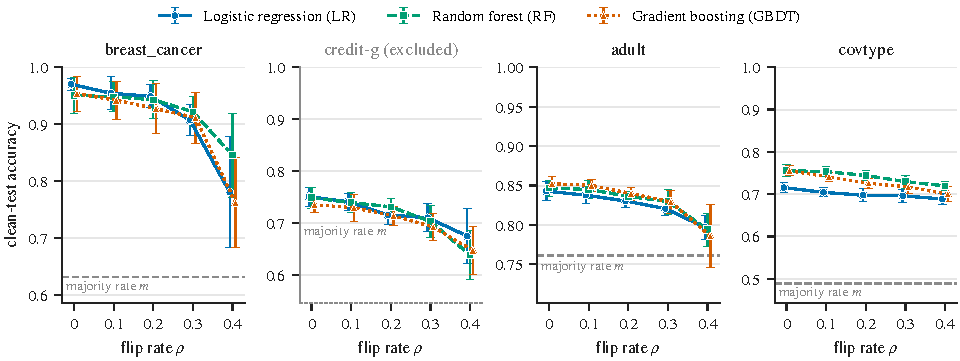
\includegraphics[width=\textwidth]{figures/fig_accuracy.pdf}
\caption{Clean-test accuracy against the training-label flip rate $\rho$, for each dataset
and method. Each point is the mean over 10 seeds, and the error bars are $\pm 1$ SD across
seeds (the seed spread, not a confidence interval). Within a seed, the split, the test set
and the nested flip sets are shared across methods and rates. Points are shifted slightly
sideways so the bars do not overlap. The dashed gray line is the majority-class rate $m$.
Test sets have 114 (\bc), 200 (\cg) and 1,000 (\ad, \ct) rows. \cg{} (dashed frame) was
excluded before any noisy run, and its curves are descriptive only.}
\label{fig:accuracy}
\end{figure}

Figure~\ref{fig:accuracy} shows accuracy at every rate, and Table~\ref{tab:accuracy} in the
appendix gives the means and SDs. Every method on every dataset is less accurate at
$\rho=0.4$ than at $\rho=0$. The ranking of the methods at each rate is descriptive only, and a
gap whose paired interval contains 0 is labelled ``within noise''. On \ct{}, RF is ahead of
GBDT, and GBDT ahead of LR, at every rate from $\rho = 0.1$ on, and each of these gaps
excludes 0. At $\rho=0$, GBDT and RF are within noise of each other. On \ad{}, LR is below
both tree methods at $\rho$ from 0.1 to 0.3, with intervals that exclude 0. At $\rho=0.4$
the order is LR, RF, GBDT, but every gap is within noise. On \bc{} and \cg{} the order
changes between rates, but every gap at every rate is within noise.

Table~\ref{tab:hyper} in the appendix gives the tuned hyperparameters at each rate. The
median selected $C$ of LR is smaller at $\rho=0.4$ than at $\rho=0$ on all four datasets:
\bc{} from $\CBcZero$ to $\CBcFour$, \cg{} from $\CCgZero$ to $\CCgFour$, \ad{} from
$\CAdZero$ to $\CAdFour$, and \ct{} from $\CCtZero$ to $\CCtFour$. The path between the
endpoints is not monotone on every dataset. What sets \ct{} apart is the level: there the
selected $C$ stays around an order of magnitude larger (weaker regularization) than on the
other three datasets at $\rho=0.4$. Stronger regularization under noise is
the direction in which \citet{vanrooyen2015} would predict robustness, but we did not test
whether it explains LR's drops. The median RF \texttt{min\_samples\_leaf} rises, for example
on \ad{} from $\MslAdZero$ to $\MslAdFour$. The median number of GBDT boosting iterations
falls on \bc{} from $\IterBcZero$ to $\IterBcFour$.

\subsection{H1: gradient boosting against the random forest}

\begin{table}[!htbp]
\centering
\small
% Generated by code/tab_h1h2.py from logged runs. Do not edit by hand; rerun the script.
% Needs \usepackage{booktabs,array} and % Generated by `crew.py numbers` from claims.jsonl. Do not edit by hand.
% Each macro is a number taken from a logged run; see claims.jsonl.
\newcommand{\NCells}{600}  % c-n-cells
\newcommand{\NFlipFail}{0}  % c-flip-fail
\newcommand{\NConvWarnCells}{0}  % c-convwarn
\newcommand{\MajBc}{0.632}  % c-m-Bc
\newcommand{\AccBcLrZero}{0.970}  % c-acc-Bc-Lr-Zero
\newcommand{\SdBcLrZero}{0.010}  % c-sd-Bc-Lr-Zero
\newcommand{\PmsBcLrZero}{0.651}  % c-pms-Bc-Lr-Zero
\newcommand{\VnBcLrZero}{0.975}  % c-vn-Bc-Lr-Zero
\newcommand{\VcBcLrZero}{0.975}  % c-vc-Bc-Lr-Zero
\newcommand{\TnBcLrZero}{0.987}  % c-tn-Bc-Lr-Zero
\newcommand{\CBcZero}{0.276}  % c-C-Bc-Zero
\newcommand{\AccBcLrOne}{0.954}  % c-acc-Bc-Lr-One
\newcommand{\SdBcLrOne}{0.029}  % c-sd-Bc-Lr-One
\newcommand{\PmsBcLrOne}{0.665}  % c-pms-Bc-Lr-One
\newcommand{\VnBcLrOne}{0.875}  % c-vn-Bc-Lr-One
\newcommand{\VcBcLrOne}{0.954}  % c-vc-Bc-Lr-One
\newcommand{\TnBcLrOne}{0.875}  % c-tn-Bc-Lr-One
\newcommand{\CBcOne}{0.104}  % c-C-Bc-One
\newcommand{\AccBcLrTwo}{0.949}  % c-acc-Bc-Lr-Two
\newcommand{\SdBcLrTwo}{0.020}  % c-sd-Bc-Lr-Two
\newcommand{\PmsBcLrTwo}{0.667}  % c-pms-Bc-Lr-Two
\newcommand{\VnBcLrTwo}{0.777}  % c-vn-Bc-Lr-Two
\newcommand{\VcBcLrTwo}{0.953}  % c-vc-Bc-Lr-Two
\newcommand{\TnBcLrTwo}{0.777}  % c-tn-Bc-Lr-Two
\newcommand{\CBcTwo}{0.0492}  % c-C-Bc-Two
\newcommand{\AccBcLrThree}{0.907}  % c-acc-Bc-Lr-Three
\newcommand{\SdBcLrThree}{0.027}  % c-sd-Bc-Lr-Three
\newcommand{\PmsBcLrThree}{0.672}  % c-pms-Bc-Lr-Three
\newcommand{\VnBcLrThree}{0.689}  % c-vn-Bc-Lr-Three
\newcommand{\VcBcLrThree}{0.909}  % c-vc-Bc-Lr-Three
\newcommand{\TnBcLrThree}{0.684}  % c-tn-Bc-Lr-Three
\newcommand{\CBcThree}{0.051}  % c-C-Bc-Three
\newcommand{\AccBcLrFour}{0.781}  % c-acc-Bc-Lr-Four
\newcommand{\SdBcLrFour}{0.098}  % c-sd-Bc-Lr-Four
\newcommand{\PmsBcLrFour}{0.670}  % c-pms-Bc-Lr-Four
\newcommand{\VnBcLrFour}{0.597}  % c-vn-Bc-Lr-Four
\newcommand{\VcBcLrFour}{0.764}  % c-vc-Bc-Lr-Four
\newcommand{\TnBcLrFour}{0.593}  % c-tn-Bc-Lr-Four
\newcommand{\CBcFour}{0.0428}  % c-C-Bc-Four
\newcommand{\AccBcRfZero}{0.951}  % c-acc-Bc-Rf-Zero
\newcommand{\SdBcRfZero}{0.032}  % c-sd-Bc-Rf-Zero
\newcommand{\PmsBcRfZero}{0.633}  % c-pms-Bc-Rf-Zero
\newcommand{\VnBcRfZero}{0.961}  % c-vn-Bc-Rf-Zero
\newcommand{\VcBcRfZero}{0.961}  % c-vc-Bc-Rf-Zero
\newcommand{\TnBcRfZero}{0.988}  % c-tn-Bc-Rf-Zero
\newcommand{\MslBcZero}{2.5}  % c-msl-Bc-Zero
\newcommand{\MfBcZero}{0.24}  % c-mf-Bc-Zero
\newcommand{\AccBcRfOne}{0.948}  % c-acc-Bc-Rf-One
\newcommand{\SdBcRfOne}{0.027}  % c-sd-Bc-Rf-One
\newcommand{\PmsBcRfOne}{0.632}  % c-pms-Bc-Rf-One
\newcommand{\VnBcRfOne}{0.877}  % c-vn-Bc-Rf-One
\newcommand{\VcBcRfOne}{0.958}  % c-vc-Bc-Rf-One
\newcommand{\TnBcRfOne}{0.921}  % c-tn-Bc-Rf-One
\newcommand{\MslBcOne}{3}  % c-msl-Bc-One
\newcommand{\MfBcOne}{0.40}  % c-mf-Bc-One
\newcommand{\AccBcRfTwo}{0.943}  % c-acc-Bc-Rf-Two
\newcommand{\SdBcRfTwo}{0.033}  % c-sd-Bc-Rf-Two
\newcommand{\PmsBcRfTwo}{0.627}  % c-pms-Bc-Rf-Two
\newcommand{\VnBcRfTwo}{0.792}  % c-vn-Bc-Rf-Two
\newcommand{\VcBcRfTwo}{0.954}  % c-vc-Bc-Rf-Two
\newcommand{\TnBcRfTwo}{0.876}  % c-tn-Bc-Rf-Two
\newcommand{\MslBcTwo}{6.5}  % c-msl-Bc-Two
\newcommand{\MfBcTwo}{0.20}  % c-mf-Bc-Two
\newcommand{\AccBcRfThree}{0.922}  % c-acc-Bc-Rf-Three
\newcommand{\SdBcRfThree}{0.026}  % c-sd-Bc-Rf-Three
\newcommand{\PmsBcRfThree}{0.636}  % c-pms-Bc-Rf-Three
\newcommand{\VnBcRfThree}{0.704}  % c-vn-Bc-Rf-Three
\newcommand{\VcBcRfThree}{0.923}  % c-vc-Bc-Rf-Three
\newcommand{\TnBcRfThree}{0.764}  % c-tn-Bc-Rf-Three
\newcommand{\MslBcThree}{15}  % c-msl-Bc-Three
\newcommand{\MfBcThree}{0.49}  % c-mf-Bc-Three
\newcommand{\AccBcRfFour}{0.846}  % c-acc-Bc-Rf-Four
\newcommand{\SdBcRfFour}{0.074}  % c-sd-Bc-Rf-Four
\newcommand{\PmsBcRfFour}{0.581}  % c-pms-Bc-Rf-Four
\newcommand{\VnBcRfFour}{0.596}  % c-vn-Bc-Rf-Four
\newcommand{\VcBcRfFour}{0.834}  % c-vc-Bc-Rf-Four
\newcommand{\TnBcRfFour}{0.755}  % c-tn-Bc-Rf-Four
\newcommand{\MslBcFour}{19.5}  % c-msl-Bc-Four
\newcommand{\MfBcFour}{0.38}  % c-mf-Bc-Four
\newcommand{\AccBcGbZero}{0.954}  % c-acc-Bc-Gb-Zero
\newcommand{\SdBcGbZero}{0.031}  % c-sd-Bc-Gb-Zero
\newcommand{\PmsBcGbZero}{0.632}  % c-pms-Bc-Gb-Zero
\newcommand{\VnBcGbZero}{0.975}  % c-vn-Bc-Gb-Zero
\newcommand{\VcBcGbZero}{0.975}  % c-vc-Bc-Gb-Zero
\newcommand{\TnBcGbZero}{1.000}  % c-tn-Bc-Gb-Zero
\newcommand{\LrateBcZero}{0.057}  % c-lrate-Bc-Zero
\newcommand{\IterBcZero}{167}  % c-iter-Bc-Zero
\newcommand{\AccBcGbOne}{0.942}  % c-acc-Bc-Gb-One
\newcommand{\SdBcGbOne}{0.033}  % c-sd-Bc-Gb-One
\newcommand{\PmsBcGbOne}{0.625}  % c-pms-Bc-Gb-One
\newcommand{\VnBcGbOne}{0.882}  % c-vn-Bc-Gb-One
\newcommand{\VcBcGbOne}{0.958}  % c-vc-Bc-Gb-One
\newcommand{\TnBcGbOne}{0.964}  % c-tn-Bc-Gb-One
\newcommand{\LrateBcOne}{0.0728}  % c-lrate-Bc-One
\newcommand{\IterBcOne}{62}  % c-iter-Bc-One
\newcommand{\AccBcGbTwo}{0.927}  % c-acc-Bc-Gb-Two
\newcommand{\SdBcGbTwo}{0.044}  % c-sd-Bc-Gb-Two
\newcommand{\PmsBcGbTwo}{0.625}  % c-pms-Bc-Gb-Two
\newcommand{\VnBcGbTwo}{0.782}  % c-vn-Bc-Gb-Two
\newcommand{\VcBcGbTwo}{0.939}  % c-vc-Bc-Gb-Two
\newcommand{\TnBcGbTwo}{0.889}  % c-tn-Bc-Gb-Two
\newcommand{\LrateBcTwo}{0.0743}  % c-lrate-Bc-Two
\newcommand{\IterBcTwo}{54}  % c-iter-Bc-Two
\newcommand{\AccBcGbThree}{0.911}  % c-acc-Bc-Gb-Three
\newcommand{\SdBcGbThree}{0.045}  % c-sd-Bc-Gb-Three
\newcommand{\PmsBcGbThree}{0.629}  % c-pms-Bc-Gb-Three
\newcommand{\VnBcGbThree}{0.698}  % c-vn-Bc-Gb-Three
\newcommand{\VcBcGbThree}{0.918}  % c-vc-Bc-Gb-Three
\newcommand{\TnBcGbThree}{0.752}  % c-tn-Bc-Gb-Three
\newcommand{\LrateBcThree}{0.0233}  % c-lrate-Bc-Three
\newcommand{\IterBcThree}{82}  % c-iter-Bc-Three
\newcommand{\AccBcGbFour}{0.762}  % c-acc-Bc-Gb-Four
\newcommand{\SdBcGbFour}{0.079}  % c-sd-Bc-Gb-Four
\newcommand{\PmsBcGbFour}{0.568}  % c-pms-Bc-Gb-Four
\newcommand{\VnBcGbFour}{0.604}  % c-vn-Bc-Gb-Four
\newcommand{\VcBcGbFour}{0.756}  % c-vc-Bc-Gb-Four
\newcommand{\TnBcGbFour}{0.800}  % c-tn-Bc-Gb-Four
\newcommand{\LrateBcFour}{0.0717}  % c-lrate-Bc-Four
\newcommand{\IterBcFour}{31}  % c-iter-Bc-Four
\newcommand{\MajCg}{0.700}  % c-m-Cg
\newcommand{\AccCgLrZero}{0.750}  % c-acc-Cg-Lr-Zero
\newcommand{\SdCgLrZero}{0.018}  % c-sd-Cg-Lr-Zero
\newcommand{\PmsCgLrZero}{0.795}  % c-pms-Cg-Lr-Zero
\newcommand{\VnCgLrZero}{0.762}  % c-vn-Cg-Lr-Zero
\newcommand{\VcCgLrZero}{0.762}  % c-vc-Cg-Lr-Zero
\newcommand{\TnCgLrZero}{0.788}  % c-tn-Cg-Lr-Zero
\newcommand{\CCgZero}{0.272}  % c-C-Cg-Zero
\newcommand{\AccCgLrOne}{0.741}  % c-acc-Cg-Lr-One
\newcommand{\SdCgLrOne}{0.016}  % c-sd-Cg-Lr-One
\newcommand{\PmsCgLrOne}{0.793}  % c-pms-Cg-Lr-One
\newcommand{\VnCgLrOne}{0.718}  % c-vn-Cg-Lr-One
\newcommand{\VcCgLrOne}{0.758}  % c-vc-Cg-Lr-One
\newcommand{\TnCgLrOne}{0.739}  % c-tn-Cg-Lr-One
\newcommand{\CCgOne}{0.255}  % c-C-Cg-One
\newcommand{\AccCgLrTwo}{0.715}  % c-acc-Cg-Lr-Two
\newcommand{\SdCgLrTwo}{0.019}  % c-sd-Cg-Lr-Two
\newcommand{\PmsCgLrTwo}{0.839}  % c-pms-Cg-Lr-Two
\newcommand{\VnCgLrTwo}{0.666}  % c-vn-Cg-Lr-Two
\newcommand{\VcCgLrTwo}{0.734}  % c-vc-Cg-Lr-Two
\newcommand{\TnCgLrTwo}{0.677}  % c-tn-Cg-Lr-Two
\newcommand{\CCgTwo}{0.0654}  % c-C-Cg-Two
\newcommand{\AccCgLrThree}{0.710}  % c-acc-Cg-Lr-Three
\newcommand{\SdCgLrThree}{0.028}  % c-sd-Cg-Lr-Three
\newcommand{\PmsCgLrThree}{0.839}  % c-pms-Cg-Lr-Three
\newcommand{\VnCgLrThree}{0.611}  % c-vn-Cg-Lr-Three
\newcommand{\VcCgLrThree}{0.718}  % c-vc-Cg-Lr-Three
\newcommand{\TnCgLrThree}{0.635}  % c-tn-Cg-Lr-Three
\newcommand{\CCgThree}{0.0336}  % c-C-Cg-Three
\newcommand{\AccCgLrFour}{0.674}  % c-acc-Cg-Lr-Four
\newcommand{\SdCgLrFour}{0.053}  % c-sd-Cg-Lr-Four
\newcommand{\PmsCgLrFour}{0.867}  % c-pms-Cg-Lr-Four
\newcommand{\VnCgLrFour}{0.576}  % c-vn-Cg-Lr-Four
\newcommand{\VcCgLrFour}{0.683}  % c-vc-Cg-Lr-Four
\newcommand{\TnCgLrFour}{0.572}  % c-tn-Cg-Lr-Four
\newcommand{\CCgFour}{0.00698}  % c-C-Cg-Four
\newcommand{\AccCgRfZero}{0.749}  % c-acc-Cg-Rf-Zero
\newcommand{\SdCgRfZero}{0.020}  % c-sd-Cg-Rf-Zero
\newcommand{\PmsCgRfZero}{0.823}  % c-pms-Cg-Rf-Zero
\newcommand{\VnCgRfZero}{0.781}  % c-vn-Cg-Rf-Zero
\newcommand{\VcCgRfZero}{0.781}  % c-vc-Cg-Rf-Zero
\newcommand{\TnCgRfZero}{0.929}  % c-tn-Cg-Rf-Zero
\newcommand{\MslCgZero}{2}  % c-msl-Cg-Zero
\newcommand{\MfCgZero}{0.26}  % c-mf-Cg-Zero
\newcommand{\AccCgRfOne}{0.739}  % c-acc-Cg-Rf-One
\newcommand{\SdCgRfOne}{0.019}  % c-sd-Cg-Rf-One
\newcommand{\PmsCgRfOne}{0.828}  % c-pms-Cg-Rf-One
\newcommand{\VnCgRfOne}{0.725}  % c-vn-Cg-Rf-One
\newcommand{\VcCgRfOne}{0.767}  % c-vc-Cg-Rf-One
\newcommand{\TnCgRfOne}{0.882}  % c-tn-Cg-Rf-One
\newcommand{\MslCgOne}{5.5}  % c-msl-Cg-One
\newcommand{\MfCgOne}{0.29}  % c-mf-Cg-One
\newcommand{\AccCgRfTwo}{0.731}  % c-acc-Cg-Rf-Two
\newcommand{\SdCgRfTwo}{0.017}  % c-sd-Cg-Rf-Two
\newcommand{\PmsCgRfTwo}{0.815}  % c-pms-Cg-Rf-Two
\newcommand{\VnCgRfTwo}{0.681}  % c-vn-Cg-Rf-Two
\newcommand{\VcCgRfTwo}{0.753}  % c-vc-Cg-Rf-Two
\newcommand{\TnCgRfTwo}{0.853}  % c-tn-Cg-Rf-Two
\newcommand{\MslCgTwo}{4.5}  % c-msl-Cg-Two
\newcommand{\MfCgTwo}{0.28}  % c-mf-Cg-Two
\newcommand{\AccCgRfThree}{0.703}  % c-acc-Cg-Rf-Three
\newcommand{\SdCgRfThree}{0.031}  % c-sd-Cg-Rf-Three
\newcommand{\PmsCgRfThree}{0.843}  % c-pms-Cg-Rf-Three
\newcommand{\VnCgRfThree}{0.629}  % c-vn-Cg-Rf-Three
\newcommand{\VcCgRfThree}{0.725}  % c-vc-Cg-Rf-Three
\newcommand{\TnCgRfThree}{0.773}  % c-tn-Cg-Rf-Three
\newcommand{\MslCgThree}{9}  % c-msl-Cg-Three
\newcommand{\MfCgThree}{0.30}  % c-mf-Cg-Three
\newcommand{\AccCgRfFour}{0.638}  % c-acc-Cg-Rf-Four
\newcommand{\SdCgRfFour}{0.047}  % c-sd-Cg-Rf-Four
\newcommand{\PmsCgRfFour}{0.728}  % c-pms-Cg-Rf-Four
\newcommand{\VnCgRfFour}{0.585}  % c-vn-Cg-Rf-Four
\newcommand{\VcCgRfFour}{0.661}  % c-vc-Cg-Rf-Four
\newcommand{\TnCgRfFour}{0.732}  % c-tn-Cg-Rf-Four
\newcommand{\MslCgFour}{15.5}  % c-msl-Cg-Four
\newcommand{\MfCgFour}{0.32}  % c-mf-Cg-Four
\newcommand{\AccCgGbZero}{0.735}  % c-acc-Cg-Gb-Zero
\newcommand{\SdCgGbZero}{0.016}  % c-sd-Cg-Gb-Zero
\newcommand{\PmsCgGbZero}{0.791}  % c-pms-Cg-Gb-Zero
\newcommand{\VnCgGbZero}{0.783}  % c-vn-Cg-Gb-Zero
\newcommand{\VcCgGbZero}{0.783}  % c-vc-Cg-Gb-Zero
\newcommand{\TnCgGbZero}{0.932}  % c-tn-Cg-Gb-Zero
\newcommand{\LrateCgZero}{0.158}  % c-lrate-Cg-Zero
\newcommand{\IterCgZero}{56}  % c-iter-Cg-Zero
\newcommand{\AccCgGbOne}{0.729}  % c-acc-Cg-Gb-One
\newcommand{\SdCgGbOne}{0.026}  % c-sd-Cg-Gb-One
\newcommand{\PmsCgGbOne}{0.779}  % c-pms-Cg-Gb-One
\newcommand{\VnCgGbOne}{0.730}  % c-vn-Cg-Gb-One
\newcommand{\VcCgGbOne}{0.764}  % c-vc-Cg-Gb-One
\newcommand{\TnCgGbOne}{0.856}  % c-tn-Cg-Gb-One
\newcommand{\LrateCgOne}{0.044}  % c-lrate-Cg-One
\newcommand{\IterCgOne}{76}  % c-iter-Cg-One
\newcommand{\AccCgGbTwo}{0.714}  % c-acc-Cg-Gb-Two
\newcommand{\SdCgGbTwo}{0.018}  % c-sd-Cg-Gb-Two
\newcommand{\PmsCgGbTwo}{0.797}  % c-pms-Cg-Gb-Two
\newcommand{\VnCgGbTwo}{0.684}  % c-vn-Cg-Gb-Two
\newcommand{\VcCgGbTwo}{0.742}  % c-vc-Cg-Gb-Two
\newcommand{\TnCgGbTwo}{0.793}  % c-tn-Cg-Gb-Two
\newcommand{\LrateCgTwo}{0.0254}  % c-lrate-Cg-Two
\newcommand{\IterCgTwo}{102}  % c-iter-Cg-Two
\newcommand{\AccCgGbThree}{0.692}  % c-acc-Cg-Gb-Three
\newcommand{\SdCgGbThree}{0.027}  % c-sd-Cg-Gb-Three
\newcommand{\PmsCgGbThree}{0.793}  % c-pms-Cg-Gb-Three
\newcommand{\VnCgGbThree}{0.626}  % c-vn-Cg-Gb-Three
\newcommand{\VcCgGbThree}{0.705}  % c-vc-Cg-Gb-Three
\newcommand{\TnCgGbThree}{0.728}  % c-tn-Cg-Gb-Three
\newcommand{\LrateCgThree}{0.0316}  % c-lrate-Cg-Three
\newcommand{\IterCgThree}{53}  % c-iter-Cg-Three
\newcommand{\AccCgGbFour}{0.647}  % c-acc-Cg-Gb-Four
\newcommand{\SdCgGbFour}{0.046}  % c-sd-Cg-Gb-Four
\newcommand{\PmsCgGbFour}{0.783}  % c-pms-Cg-Gb-Four
\newcommand{\VnCgGbFour}{0.581}  % c-vn-Cg-Gb-Four
\newcommand{\VcCgGbFour}{0.651}  % c-vc-Cg-Gb-Four
\newcommand{\TnCgGbFour}{0.667}  % c-tn-Cg-Gb-Four
\newcommand{\LrateCgFour}{0.0251}  % c-lrate-Cg-Four
\newcommand{\IterCgFour}{29}  % c-iter-Cg-Four
\newcommand{\MajAd}{0.761}  % c-m-Ad
\newcommand{\AccAdLrZero}{0.843}  % c-acc-Ad-Lr-Zero
\newcommand{\SdAdLrZero}{0.012}  % c-sd-Ad-Lr-Zero
\newcommand{\PmsAdLrZero}{0.812}  % c-pms-Ad-Lr-Zero
\newcommand{\VnAdLrZero}{0.849}  % c-vn-Ad-Lr-Zero
\newcommand{\VcAdLrZero}{0.849}  % c-vc-Ad-Lr-Zero
\newcommand{\TnAdLrZero}{0.855}  % c-tn-Ad-Lr-Zero
\newcommand{\CAdZero}{0.38}  % c-C-Ad-Zero
\newcommand{\AccAdLrOne}{0.838}  % c-acc-Ad-Lr-One
\newcommand{\SdAdLrOne}{0.010}  % c-sd-Ad-Lr-One
\newcommand{\PmsAdLrOne}{0.822}  % c-pms-Ad-Lr-One
\newcommand{\VnAdLrOne}{0.776}  % c-vn-Ad-Lr-One
\newcommand{\VcAdLrOne}{0.844}  % c-vc-Ad-Lr-One
\newcommand{\TnAdLrOne}{0.780}  % c-tn-Ad-Lr-One
\newcommand{\CAdOne}{0.182}  % c-C-Ad-One
\newcommand{\AccAdLrTwo}{0.830}  % c-acc-Ad-Lr-Two
\newcommand{\SdAdLrTwo}{0.009}  % c-sd-Ad-Lr-Two
\newcommand{\PmsAdLrTwo}{0.848}  % c-pms-Ad-Lr-Two
\newcommand{\VnAdLrTwo}{0.703}  % c-vn-Ad-Lr-Two
\newcommand{\VcAdLrTwo}{0.833}  % c-vc-Ad-Lr-Two
\newcommand{\TnAdLrTwo}{0.703}  % c-tn-Ad-Lr-Two
\newcommand{\CAdTwo}{0.0195}  % c-C-Ad-Two
\newcommand{\AccAdLrThree}{0.821}  % c-acc-Ad-Lr-Three
\newcommand{\SdAdLrThree}{0.009}  % c-sd-Ad-Lr-Three
\newcommand{\PmsAdLrThree}{0.847}  % c-pms-Ad-Lr-Three
\newcommand{\VnAdLrThree}{0.637}  % c-vn-Ad-Lr-Three
\newcommand{\VcAdLrThree}{0.823}  % c-vc-Ad-Lr-Three
\newcommand{\TnAdLrThree}{0.637}  % c-tn-Ad-Lr-Three
\newcommand{\CAdThree}{0.0202}  % c-C-Ad-Three
\newcommand{\AccAdLrFour}{0.797}  % c-acc-Ad-Lr-Four
\newcommand{\SdAdLrFour}{0.015}  % c-sd-Ad-Lr-Four
\newcommand{\PmsAdLrFour}{0.833}  % c-pms-Ad-Lr-Four
\newcommand{\VnAdLrFour}{0.569}  % c-vn-Ad-Lr-Four
\newcommand{\VcAdLrFour}{0.804}  % c-vc-Ad-Lr-Four
\newcommand{\TnAdLrFour}{0.572}  % c-tn-Ad-Lr-Four
\newcommand{\CAdFour}{0.00584}  % c-C-Ad-Four
\newcommand{\AccAdRfZero}{0.847}  % c-acc-Ad-Rf-Zero
\newcommand{\SdAdRfZero}{0.010}  % c-sd-Ad-Rf-Zero
\newcommand{\PmsAdRfZero}{0.814}  % c-pms-Ad-Rf-Zero
\newcommand{\VnAdRfZero}{0.859}  % c-vn-Ad-Rf-Zero
\newcommand{\VcAdRfZero}{0.859}  % c-vc-Ad-Rf-Zero
\newcommand{\TnAdRfZero}{0.911}  % c-tn-Ad-Rf-Zero
\newcommand{\MslAdZero}{3}  % c-msl-Ad-Zero
\newcommand{\MfAdZero}{0.20}  % c-mf-Ad-Zero
\newcommand{\AccAdRfOne}{0.845}  % c-acc-Ad-Rf-One
\newcommand{\SdAdRfOne}{0.012}  % c-sd-Ad-Rf-One
\newcommand{\PmsAdRfOne}{0.812}  % c-pms-Ad-Rf-One
\newcommand{\VnAdRfOne}{0.788}  % c-vn-Ad-Rf-One
\newcommand{\VcAdRfOne}{0.855}  % c-vc-Ad-Rf-One
\newcommand{\TnAdRfOne}{0.829}  % c-tn-Ad-Rf-One
\newcommand{\MslAdOne}{3.5}  % c-msl-Ad-One
\newcommand{\MfAdOne}{0.22}  % c-mf-Ad-One
\newcommand{\AccAdRfTwo}{0.836}  % c-acc-Ad-Rf-Two
\newcommand{\SdAdRfTwo}{0.006}  % c-sd-Ad-Rf-Two
\newcommand{\PmsAdRfTwo}{0.823}  % c-pms-Ad-Rf-Two
\newcommand{\VnAdRfTwo}{0.714}  % c-vn-Ad-Rf-Two
\newcommand{\VcAdRfTwo}{0.847}  % c-vc-Ad-Rf-Two
\newcommand{\TnAdRfTwo}{0.760}  % c-tn-Ad-Rf-Two
\newcommand{\MslAdTwo}{2.5}  % c-msl-Ad-Two
\newcommand{\MfAdTwo}{0.11}  % c-mf-Ad-Two
\newcommand{\AccAdRfThree}{0.830}  % c-acc-Ad-Rf-Three
\newcommand{\SdAdRfThree}{0.016}  % c-sd-Ad-Rf-Three
\newcommand{\PmsAdRfThree}{0.809}  % c-pms-Ad-Rf-Three
\newcommand{\VnAdRfThree}{0.644}  % c-vn-Ad-Rf-Three
\newcommand{\VcAdRfThree}{0.834}  % c-vc-Ad-Rf-Three
\newcommand{\TnAdRfThree}{0.715}  % c-tn-Ad-Rf-Three
\newcommand{\MslAdThree}{11}  % c-msl-Ad-Three
\newcommand{\MfAdThree}{0.13}  % c-mf-Ad-Three
\newcommand{\AccAdRfFour}{0.794}  % c-acc-Ad-Rf-Four
\newcommand{\SdAdRfFour}{0.021}  % c-sd-Ad-Rf-Four
\newcommand{\PmsAdRfFour}{0.776}  % c-pms-Ad-Rf-Four
\newcommand{\VnAdRfFour}{0.571}  % c-vn-Ad-Rf-Four
\newcommand{\VcAdRfFour}{0.804}  % c-vc-Ad-Rf-Four
\newcommand{\TnAdRfFour}{0.646}  % c-tn-Ad-Rf-Four
\newcommand{\MslAdFour}{23}  % c-msl-Ad-Four
\newcommand{\MfAdFour}{0.28}  % c-mf-Ad-Four
\newcommand{\AccAdGbZero}{0.852}  % c-acc-Ad-Gb-Zero
\newcommand{\SdAdGbZero}{0.009}  % c-sd-Ad-Gb-Zero
\newcommand{\PmsAdGbZero}{0.803}  % c-pms-Ad-Gb-Zero
\newcommand{\VnAdGbZero}{0.866}  % c-vn-Ad-Gb-Zero
\newcommand{\VcAdGbZero}{0.866}  % c-vc-Ad-Gb-Zero
\newcommand{\TnAdGbZero}{0.907}  % c-tn-Ad-Gb-Zero
\newcommand{\LrateAdZero}{0.109}  % c-lrate-Ad-Zero
\newcommand{\IterAdZero}{94}  % c-iter-Ad-Zero
\newcommand{\AccAdGbOne}{0.850}  % c-acc-Ad-Gb-One
\newcommand{\SdAdGbOne}{0.007}  % c-sd-Ad-Gb-One
\newcommand{\PmsAdGbOne}{0.821}  % c-pms-Ad-Gb-One
\newcommand{\VnAdGbOne}{0.792}  % c-vn-Ad-Gb-One
\newcommand{\VcAdGbOne}{0.861}  % c-vc-Ad-Gb-One
\newcommand{\TnAdGbOne}{0.813}  % c-tn-Ad-Gb-One
\newcommand{\LrateAdOne}{0.0201}  % c-lrate-Ad-One
\newcommand{\IterAdOne}{173}  % c-iter-Ad-One
\newcommand{\AccAdGbTwo}{0.840}  % c-acc-Ad-Gb-Two
\newcommand{\SdAdGbTwo}{0.008}  % c-sd-Ad-Gb-Two
\newcommand{\PmsAdGbTwo}{0.822}  % c-pms-Ad-Gb-Two
\newcommand{\VnAdGbTwo}{0.717}  % c-vn-Ad-Gb-Two
\newcommand{\VcAdGbTwo}{0.853}  % c-vc-Ad-Gb-Two
\newcommand{\TnAdGbTwo}{0.749}  % c-tn-Ad-Gb-Two
\newcommand{\LrateAdTwo}{0.0229}  % c-lrate-Ad-Two
\newcommand{\IterAdTwo}{120}  % c-iter-Ad-Two
\newcommand{\AccAdGbThree}{0.829}  % c-acc-Ad-Gb-Three
\newcommand{\SdAdGbThree}{0.014}  % c-sd-Ad-Gb-Three
\newcommand{\PmsAdGbThree}{0.829}  % c-pms-Ad-Gb-Three
\newcommand{\VnAdGbThree}{0.646}  % c-vn-Ad-Gb-Three
\newcommand{\VcAdGbThree}{0.838}  % c-vc-Ad-Gb-Three
\newcommand{\TnAdGbThree}{0.682}  % c-tn-Ad-Gb-Three
\newcommand{\LrateAdThree}{0.0257}  % c-lrate-Ad-Three
\newcommand{\IterAdThree}{86}  % c-iter-Ad-Three
\newcommand{\AccAdGbFour}{0.786}  % c-acc-Ad-Gb-Four
\newcommand{\SdAdGbFour}{0.040}  % c-sd-Ad-Gb-Four
\newcommand{\PmsAdGbFour}{0.842}  % c-pms-Ad-Gb-Four
\newcommand{\VnAdGbFour}{0.571}  % c-vn-Ad-Gb-Four
\newcommand{\VcAdGbFour}{0.795}  % c-vc-Ad-Gb-Four
\newcommand{\TnAdGbFour}{0.606}  % c-tn-Ad-Gb-Four
\newcommand{\LrateAdFour}{0.0169}  % c-lrate-Ad-Four
\newcommand{\IterAdFour}{64}  % c-iter-Ad-Four
\newcommand{\MajCt}{0.488}  % c-m-Ct
\newcommand{\AccCtLrZero}{0.715}  % c-acc-Ct-Lr-Zero
\newcommand{\SdCtLrZero}{0.011}  % c-sd-Ct-Lr-Zero
\newcommand{\PmsCtLrZero}{0.526}  % c-pms-Ct-Lr-Zero
\newcommand{\VnCtLrZero}{0.718}  % c-vn-Ct-Lr-Zero
\newcommand{\VcCtLrZero}{0.718}  % c-vc-Ct-Lr-Zero
\newcommand{\TnCtLrZero}{0.736}  % c-tn-Ct-Lr-Zero
\newcommand{\CCtZero}{2.25}  % c-C-Ct-Zero
\newcommand{\AccCtLrOne}{0.704}  % c-acc-Ct-Lr-One
\newcommand{\SdCtLrOne}{0.011}  % c-sd-Ct-Lr-One
\newcommand{\PmsCtLrOne}{0.540}  % c-pms-Ct-Lr-One
\newcommand{\VnCtLrOne}{0.645}  % c-vn-Ct-Lr-One
\newcommand{\VcCtLrOne}{0.710}  % c-vc-Ct-Lr-One
\newcommand{\TnCtLrOne}{0.656}  % c-tn-Ct-Lr-One
\newcommand{\CCtOne}{2.75}  % c-C-Ct-One
\newcommand{\AccCtLrTwo}{0.697}  % c-acc-Ct-Lr-Two
\newcommand{\SdCtLrTwo}{0.016}  % c-sd-Ct-Lr-Two
\newcommand{\PmsCtLrTwo}{0.544}  % c-pms-Ct-Lr-Two
\newcommand{\VnCtLrTwo}{0.576}  % c-vn-Ct-Lr-Two
\newcommand{\VcCtLrTwo}{0.703}  % c-vc-Ct-Lr-Two
\newcommand{\TnCtLrTwo}{0.586}  % c-tn-Ct-Lr-Two
\newcommand{\CCtTwo}{0.336}  % c-C-Ct-Two
\newcommand{\AccCtLrThree}{0.696}  % c-acc-Ct-Lr-Three
\newcommand{\SdCtLrThree}{0.015}  % c-sd-Ct-Lr-Three
\newcommand{\PmsCtLrThree}{0.550}  % c-pms-Ct-Lr-Three
\newcommand{\VnCtLrThree}{0.509}  % c-vn-Ct-Lr-Three
\newcommand{\VcCtLrThree}{0.697}  % c-vc-Ct-Lr-Three
\newcommand{\TnCtLrThree}{0.515}  % c-tn-Ct-Lr-Three
\newcommand{\CCtThree}{4.04}  % c-C-Ct-Three
\newcommand{\AccCtLrFour}{0.689}  % c-acc-Ct-Lr-Four
\newcommand{\SdCtLrFour}{0.014}  % c-sd-Ct-Lr-Four
\newcommand{\PmsCtLrFour}{0.555}  % c-pms-Ct-Lr-Four
\newcommand{\VnCtLrFour}{0.436}  % c-vn-Ct-Lr-Four
\newcommand{\VcCtLrFour}{0.688}  % c-vc-Ct-Lr-Four
\newcommand{\TnCtLrFour}{0.450}  % c-tn-Ct-Lr-Four
\newcommand{\CCtFour}{0.62}  % c-C-Ct-Four
\newcommand{\AccCtRfZero}{0.755}  % c-acc-Ct-Rf-Zero
\newcommand{\SdCtRfZero}{0.014}  % c-sd-Ct-Rf-Zero
\newcommand{\PmsCtRfZero}{0.523}  % c-pms-Ct-Rf-Zero
\newcommand{\VnCtRfZero}{0.760}  % c-vn-Ct-Rf-Zero
\newcommand{\VcCtRfZero}{0.760}  % c-vc-Ct-Rf-Zero
\newcommand{\TnCtRfZero}{0.992}  % c-tn-Ct-Rf-Zero
\newcommand{\MslCtZero}{1}  % c-msl-Ct-Zero
\newcommand{\MfCtZero}{0.45}  % c-mf-Ct-Zero
\newcommand{\AccCtRfOne}{0.753}  % c-acc-Ct-Rf-One
\newcommand{\SdCtRfOne}{0.012}  % c-sd-Ct-Rf-One
\newcommand{\PmsCtRfOne}{0.529}  % c-pms-Ct-Rf-One
\newcommand{\VnCtRfOne}{0.687}  % c-vn-Ct-Rf-One
\newcommand{\VcCtRfOne}{0.759}  % c-vc-Ct-Rf-One
\newcommand{\TnCtRfOne}{0.976}  % c-tn-Ct-Rf-One
\newcommand{\MslCtOne}{1}  % c-msl-Ct-One
\newcommand{\MfCtOne}{0.42}  % c-mf-Ct-One
\newcommand{\AccCtRfTwo}{0.744}  % c-acc-Ct-Rf-Two
\newcommand{\SdCtRfTwo}{0.012}  % c-sd-Ct-Rf-Two
\newcommand{\PmsCtRfTwo}{0.534}  % c-pms-Ct-Rf-Two
\newcommand{\VnCtRfTwo}{0.609}  % c-vn-Ct-Rf-Two
\newcommand{\VcCtRfTwo}{0.754}  % c-vc-Ct-Rf-Two
\newcommand{\TnCtRfTwo}{0.960}  % c-tn-Ct-Rf-Two
\newcommand{\MslCtTwo}{1.5}  % c-msl-Ct-Two
\newcommand{\MfCtTwo}{0.37}  % c-mf-Ct-Two
\newcommand{\AccCtRfThree}{0.730}  % c-acc-Ct-Rf-Three
\newcommand{\SdCtRfThree}{0.016}  % c-sd-Ct-Rf-Three
\newcommand{\PmsCtRfThree}{0.531}  % c-pms-Ct-Rf-Three
\newcommand{\VnCtRfThree}{0.533}  % c-vn-Ct-Rf-Three
\newcommand{\VcCtRfThree}{0.739}  % c-vc-Ct-Rf-Three
\newcommand{\TnCtRfThree}{0.758}  % c-tn-Ct-Rf-Three
\newcommand{\MslCtThree}{3.5}  % c-msl-Ct-Three
\newcommand{\MfCtThree}{0.37}  % c-mf-Ct-Three
\newcommand{\AccCtRfFour}{0.719}  % c-acc-Ct-Rf-Four
\newcommand{\SdCtRfFour}{0.011}  % c-sd-Ct-Rf-Four
\newcommand{\PmsCtRfFour}{0.539}  % c-pms-Ct-Rf-Four
\newcommand{\VnCtRfFour}{0.454}  % c-vn-Ct-Rf-Four
\newcommand{\VcCtRfFour}{0.726}  % c-vc-Ct-Rf-Four
\newcommand{\TnCtRfFour}{0.774}  % c-tn-Ct-Rf-Four
\newcommand{\MslCtFour}{2.5}  % c-msl-Ct-Four
\newcommand{\MfCtFour}{0.36}  % c-mf-Ct-Four
\newcommand{\AccCtGbZero}{0.755}  % c-acc-Ct-Gb-Zero
\newcommand{\SdCtGbZero}{0.012}  % c-sd-Ct-Gb-Zero
\newcommand{\PmsCtGbZero}{0.525}  % c-pms-Ct-Gb-Zero
\newcommand{\VnCtGbZero}{0.755}  % c-vn-Ct-Gb-Zero
\newcommand{\VcCtGbZero}{0.755}  % c-vc-Ct-Gb-Zero
\newcommand{\TnCtGbZero}{0.962}  % c-tn-Ct-Gb-Zero
\newcommand{\LrateCtZero}{0.0393}  % c-lrate-Ct-Zero
\newcommand{\IterCtZero}{89}  % c-iter-Ct-Zero
\newcommand{\AccCtGbOne}{0.740}  % c-acc-Ct-Gb-One
\newcommand{\SdCtGbOne}{0.010}  % c-sd-Ct-Gb-One
\newcommand{\PmsCtGbOne}{0.531}  % c-pms-Ct-Gb-One
\newcommand{\VnCtGbOne}{0.677}  % c-vn-Ct-Gb-One
\newcommand{\VcCtGbOne}{0.746}  % c-vc-Ct-Gb-One
\newcommand{\TnCtGbOne}{0.939}  % c-tn-Ct-Gb-One
\newcommand{\LrateCtOne}{0.0341}  % c-lrate-Ct-One
\newcommand{\IterCtOne}{84}  % c-iter-Ct-One
\newcommand{\AccCtGbTwo}{0.726}  % c-acc-Ct-Gb-Two
\newcommand{\SdCtGbTwo}{0.012}  % c-sd-Ct-Gb-Two
\newcommand{\PmsCtGbTwo}{0.536}  % c-pms-Ct-Gb-Two
\newcommand{\VnCtGbTwo}{0.600}  % c-vn-Ct-Gb-Two
\newcommand{\VcCtGbTwo}{0.736}  % c-vc-Ct-Gb-Two
\newcommand{\TnCtGbTwo}{0.788}  % c-tn-Ct-Gb-Two
\newcommand{\LrateCtTwo}{0.0431}  % c-lrate-Ct-Two
\newcommand{\IterCtTwo}{64}  % c-iter-Ct-Two
\newcommand{\AccCtGbThree}{0.717}  % c-acc-Ct-Gb-Three
\newcommand{\SdCtGbThree}{0.014}  % c-sd-Ct-Gb-Three
\newcommand{\PmsCtGbThree}{0.535}  % c-pms-Ct-Gb-Three
\newcommand{\VnCtGbThree}{0.525}  % c-vn-Ct-Gb-Three
\newcommand{\VcCtGbThree}{0.724}  % c-vc-Ct-Gb-Three
\newcommand{\TnCtGbThree}{0.633}  % c-tn-Ct-Gb-Three
\newcommand{\LrateCtThree}{0.0603}  % c-lrate-Ct-Three
\newcommand{\IterCtThree}{56}  % c-iter-Ct-Three
\newcommand{\AccCtGbFour}{0.700}  % c-acc-Ct-Gb-Four
\newcommand{\SdCtGbFour}{0.018}  % c-sd-Ct-Gb-Four
\newcommand{\PmsCtGbFour}{0.545}  % c-pms-Ct-Gb-Four
\newcommand{\VnCtGbFour}{0.451}  % c-vn-Ct-Gb-Four
\newcommand{\VcCtGbFour}{0.710}  % c-vc-Ct-Gb-Four
\newcommand{\TnCtGbFour}{0.531}  % c-tn-Ct-Gb-Four
\newcommand{\LrateCtFour}{0.0457}  % c-lrate-Ct-Four
\newcommand{\IterCtFour}{51}  % c-iter-Ct-Four
\newcommand{\HeadBcLr}{0.339}  % c-head-Bc-Lr
\newcommand{\HeadBcRf}{0.319}  % c-head-Bc-Rf
\newcommand{\HeadBcGb}{0.322}  % c-head-Bc-Gb
\newcommand{\HeadCgLr}{0.051}  % c-head-Cg-Lr
\newcommand{\HeadCgRf}{0.049}  % c-head-Cg-Rf
\newcommand{\HeadCgGb}{0.035}  % c-head-Cg-Gb
\newcommand{\HeadAdLr}{0.082}  % c-head-Ad-Lr
\newcommand{\HeadAdRf}{0.086}  % c-head-Ad-Rf
\newcommand{\HeadAdGb}{0.091}  % c-head-Ad-Gb
\newcommand{\HeadCtLr}{0.227}  % c-head-Ct-Lr
\newcommand{\HeadCtRf}{0.267}  % c-head-Ct-Rf
\newcommand{\HeadCtGb}{0.268}  % c-head-Ct-Gb
\newcommand{\NInfHOne}{3}  % c-ninf-h1
\newcommand{\NInfHTwo}{3}  % c-ninf-h2
\newcommand{\HBcLr}{0.339}  % c-h-Bc-Lr
\newcommand{\HloBcLr}{0.323}  % c-hlo-Bc-Lr
\newcommand{\DropBcLr}{0.189}  % c-drop-Bc-Lr
\newcommand{\RBcLr}{0.560}  % c-r-Bc-Lr
\newcommand{\HBcRf}{0.319}  % c-h-Bc-Rf
\newcommand{\HloBcRf}{0.272}  % c-hlo-Bc-Rf
\newcommand{\DropBcRf}{0.105}  % c-drop-Bc-Rf
\newcommand{\RBcRf}{0.330}  % c-r-Bc-Rf
\newcommand{\HBcGb}{0.322}  % c-h-Bc-Gb
\newcommand{\HloBcGb}{0.276}  % c-hlo-Bc-Gb
\newcommand{\DropBcGb}{0.191}  % c-drop-Bc-Gb
\newcommand{\RBcGb}{0.594}  % c-r-Bc-Gb
\newcommand{\HOneDBc}{0.264}  % c-h1-Bc
\newcommand{\HOneDBcLo}{-0.014}  % c-h1-Bc-lo
\newcommand{\HOneDBcHi}{0.543}  % c-h1-Bc-hi
\newcommand{\HOneDBcS}{0.187}  % c-h1-Bc-s
\newcommand{\HOneDBcHalf}{0.279}  % c-h1-Bc-half
\newcommand{\HOneDBcBootLo}{0.173}  % c-h1-Bc-blo
\newcommand{\HOneDBcBootHi}{0.390}  % c-h1-Bc-bhi
\newcommand{\HOneDdropBc}{0.086}  % c-h1-Bc-ddrop
\newcommand{\HTwoDOneBc}{-0.034}  % c-h2-Bc-d1
\newcommand{\HTwoDOneBcLo}{-0.497}  % c-h2-Bc-d1-lo
\newcommand{\HTwoDOneBcHi}{0.428}  % c-h2-Bc-d1-hi
\newcommand{\HTwoDOneBcS}{0.310}  % c-h2-Bc-d1-s
\newcommand{\HTwoDOneBcHalf}{0.463}  % c-h2-Bc-d1-half
\newcommand{\HTwoDOneBcBootLo}{-0.221}  % c-h2-Bc-d1-blo
\newcommand{\HTwoDOneBcBootHi}{0.147}  % c-h2-Bc-d1-bhi
\newcommand{\HTwoDOneDdropBc}{-0.002}  % c-h2-Bc-d1-ddrop
\newcommand{\HTwoDTwoBc}{0.230}  % c-h2-Bc-d2
\newcommand{\HTwoDTwoBcLo}{-0.189}  % c-h2-Bc-d2-lo
\newcommand{\HTwoDTwoBcHi}{0.648}  % c-h2-Bc-d2-hi
\newcommand{\HTwoDTwoBcS}{0.281}  % c-h2-Bc-d2-s
\newcommand{\HTwoDTwoBcHalf}{0.418}  % c-h2-Bc-d2-half
\newcommand{\HTwoDTwoBcBootLo}{0.081}  % c-h2-Bc-d2-blo
\newcommand{\HTwoDTwoBcBootHi}{0.412}  % c-h2-Bc-d2-bhi
\newcommand{\HTwoDTwoDdropBc}{0.084}  % c-h2-Bc-d2-ddrop
\newcommand{\HCgLr}{0.051}  % c-h-Cg-Lr
\newcommand{\HloCgLr}{0.024}  % c-hlo-Cg-Lr
\newcommand{\DropCgLr}{0.076}  % c-drop-Cg-Lr
\newcommand{\RCgLr}{1.505}  % c-r-Cg-Lr
\newcommand{\HCgRf}{0.049}  % c-h-Cg-Rf
\newcommand{\HloCgRf}{0.019}  % c-hlo-Cg-Rf
\newcommand{\DropCgRf}{0.111}  % c-drop-Cg-Rf
\newcommand{\RCgRf}{2.278}  % c-r-Cg-Rf
\newcommand{\HCgGb}{0.035}  % c-h-Cg-Gb
\newcommand{\HloCgGb}{0.011}  % c-hlo-Cg-Gb
\newcommand{\DropCgGb}{0.088}  % c-drop-Cg-Gb
\newcommand{\RCgGb}{2.514}  % c-r-Cg-Gb
\newcommand{\HOneDCg}{0.236}  % c-h1-Cg
\newcommand{\HOneDCgLo}{-1.253}  % c-h1-Cg-lo
\newcommand{\HOneDCgHi}{1.725}  % c-h1-Cg-hi
\newcommand{\HOneDCgS}{1.000}  % c-h1-Cg-s
\newcommand{\HOneDCgHalf}{1.489}  % c-h1-Cg-half
\newcommand{\HOneDCgBootLo}{-0.218}  % c-h1-Cg-blo
\newcommand{\HOneDCgBootHi}{1.198}  % c-h1-Cg-bhi
\newcommand{\HOneDdropCg}{-0.022}  % c-h1-Cg-ddrop
\newcommand{\HTwoDOneCg}{-1.009}  % c-h2-Cg-d1
\newcommand{\HTwoDOneCgLo}{-4.392}  % c-h2-Cg-d1-lo
\newcommand{\HTwoDOneCgHi}{2.373}  % c-h2-Cg-d1-hi
\newcommand{\HTwoDOneCgS}{2.271}  % c-h2-Cg-d1-s
\newcommand{\HTwoDOneCgHalf}{3.383}  % c-h2-Cg-d1-half
\newcommand{\HTwoDOneCgBootLo}{-2.792}  % c-h2-Cg-d1-blo
\newcommand{\HTwoDOneCgBootHi}{0.187}  % c-h2-Cg-d1-bhi
\newcommand{\HTwoDOneDdropCg}{-0.012}  % c-h2-Cg-d1-ddrop
\newcommand{\HTwoDTwoCg}{-0.773}  % c-h2-Cg-d2
\newcommand{\HTwoDTwoCgLo}{-3.253}  % c-h2-Cg-d2-lo
\newcommand{\HTwoDTwoCgHi}{1.706}  % c-h2-Cg-d2-hi
\newcommand{\HTwoDTwoCgS}{1.665}  % c-h2-Cg-d2-s
\newcommand{\HTwoDTwoCgHalf}{2.479}  % c-h2-Cg-d2-half
\newcommand{\HTwoDTwoCgBootLo}{-1.788}  % c-h2-Cg-d2-blo
\newcommand{\HTwoDTwoCgBootHi}{0.228}  % c-h2-Cg-d2-bhi
\newcommand{\HTwoDTwoDdropCg}{-0.035}  % c-h2-Cg-d2-ddrop
\newcommand{\HAdLr}{0.082}  % c-h-Ad-Lr
\newcommand{\HloAdLr}{0.074}  % c-hlo-Ad-Lr
\newcommand{\DropAdLr}{0.046}  % c-drop-Ad-Lr
\newcommand{\RAdLr}{0.559}  % c-r-Ad-Lr
\newcommand{\HAdRf}{0.086}  % c-h-Ad-Rf
\newcommand{\HloAdRf}{0.078}  % c-hlo-Ad-Rf
\newcommand{\DropAdRf}{0.053}  % c-drop-Ad-Rf
\newcommand{\RAdRf}{0.614}  % c-r-Ad-Rf
\newcommand{\HAdGb}{0.091}  % c-h-Ad-Gb
\newcommand{\HloAdGb}{0.085}  % c-hlo-Ad-Gb
\newcommand{\DropAdGb}{0.066}  % c-drop-Ad-Gb
\newcommand{\RAdGb}{0.726}  % c-r-Ad-Gb
\newcommand{\HOneDAd}{0.112}  % c-h1-Ad
\newcommand{\HOneDAdLo}{-0.217}  % c-h1-Ad-lo
\newcommand{\HOneDAdHi}{0.440}  % c-h1-Ad-hi
\newcommand{\HOneDAdS}{0.459}  % c-h1-Ad-s
\newcommand{\HOneDAdHalf}{0.328}  % c-h1-Ad-half
\newcommand{\HOneDAdBootLo}{-0.123}  % c-h1-Ad-blo
\newcommand{\HOneDAdBootHi}{0.410}  % c-h1-Ad-bhi
\newcommand{\HOneDdropAd}{0.014}  % c-h1-Ad-ddrop
\newcommand{\HTwoDOneAd}{-0.167}  % c-h2-Ad-d1
\newcommand{\HTwoDOneAdLo}{-0.481}  % c-h2-Ad-d1-lo
\newcommand{\HTwoDOneAdHi}{0.147}  % c-h2-Ad-d1-hi
\newcommand{\HTwoDOneAdS}{0.439}  % c-h2-Ad-d1-s
\newcommand{\HTwoDOneAdHalf}{0.314}  % c-h2-Ad-d1-half
\newcommand{\HTwoDOneAdBootLo}{-0.461}  % c-h2-Ad-d1-blo
\newcommand{\HTwoDOneAdBootHi}{0.034}  % c-h2-Ad-d1-bhi
\newcommand{\HTwoDOneDdropAd}{-0.021}  % c-h2-Ad-d1-ddrop
\newcommand{\HTwoDTwoAd}{-0.055}  % c-h2-Ad-d2
\newcommand{\HTwoDTwoAdLo}{-0.184}  % c-h2-Ad-d2-lo
\newcommand{\HTwoDTwoAdHi}{0.073}  % c-h2-Ad-d2-hi
\newcommand{\HTwoDTwoAdS}{0.180}  % c-h2-Ad-d2-s
\newcommand{\HTwoDTwoAdHalf}{0.129}  % c-h2-Ad-d2-half
\newcommand{\HTwoDTwoAdBootLo}{-0.160}  % c-h2-Ad-d2-blo
\newcommand{\HTwoDTwoAdBootHi}{0.053}  % c-h2-Ad-d2-bhi
\newcommand{\HTwoDTwoDdropAd}{-0.007}  % c-h2-Ad-d2-ddrop
\newcommand{\HCtLr}{0.227}  % c-h-Ct-Lr
\newcommand{\HloCtLr}{0.219}  % c-hlo-Ct-Lr
\newcommand{\DropCtLr}{0.027}  % c-drop-Ct-Lr
\newcommand{\RCtLr}{0.118}  % c-r-Ct-Lr
\newcommand{\HCtRf}{0.267}  % c-h-Ct-Rf
\newcommand{\HloCtRf}{0.258}  % c-hlo-Ct-Rf
\newcommand{\DropCtRf}{0.036}  % c-drop-Ct-Rf
\newcommand{\RCtRf}{0.135}  % c-r-Ct-Rf
\newcommand{\HCtGb}{0.268}  % c-h-Ct-Gb
\newcommand{\HloCtGb}{0.259}  % c-hlo-Ct-Gb
\newcommand{\DropCtGb}{0.056}  % c-drop-Ct-Gb
\newcommand{\RCtGb}{0.208}  % c-r-Ct-Gb
\newcommand{\HOneDCt}{0.073}  % c-h1-Ct
\newcommand{\HOneDCtLo}{0.022}  % c-h1-Ct-lo
\newcommand{\HOneDCtHi}{0.124}  % c-h1-Ct-hi
\newcommand{\HOneDCtS}{0.071}  % c-h1-Ct-s
\newcommand{\HOneDCtHalf}{0.051}  % c-h1-Ct-half
\newcommand{\HOneDCtBootLo}{0.032}  % c-h1-Ct-blo
\newcommand{\HOneDCtBootHi}{0.115}  % c-h1-Ct-bhi
\newcommand{\HOneDdropCt}{0.020}  % c-h1-Ct-ddrop
\newcommand{\HTwoDOneCt}{-0.090}  % c-h2-Ct-d1
\newcommand{\HTwoDOneCtLo}{-0.138}  % c-h2-Ct-d1-lo
\newcommand{\HTwoDOneCtHi}{-0.041}  % c-h2-Ct-d1-hi
\newcommand{\HTwoDOneCtS}{0.068}  % c-h2-Ct-d1-s
\newcommand{\HTwoDOneCtHalf}{0.049}  % c-h2-Ct-d1-half
\newcommand{\HTwoDOneCtBootLo}{-0.128}  % c-h2-Ct-d1-blo
\newcommand{\HTwoDOneCtBootHi}{-0.051}  % c-h2-Ct-d1-bhi
\newcommand{\HTwoDOneDdropCt}{-0.029}  % c-h2-Ct-d1-ddrop
\newcommand{\HTwoDTwoCt}{-0.016}  % c-h2-Ct-d2
\newcommand{\HTwoDTwoCtLo}{-0.059}  % c-h2-Ct-d2-lo
\newcommand{\HTwoDTwoCtHi}{0.026}  % c-h2-Ct-d2-hi
\newcommand{\HTwoDTwoCtS}{0.059}  % c-h2-Ct-d2-s
\newcommand{\HTwoDTwoCtHalf}{0.042}  % c-h2-Ct-d2-half
\newcommand{\HTwoDTwoCtBootLo}{-0.049}  % c-h2-Ct-d2-blo
\newcommand{\HTwoDTwoCtBootHi}{0.020}  % c-h2-Ct-d2-bhi
\newcommand{\HTwoDTwoDdropCt}{-0.009}  % c-h2-Ct-d2-ddrop
\newcommand{\HOneNInf}{3}  % c-h1-n_informative
\newcommand{\HOneNSup}{1}  % c-h1-n_supported
\newcommand{\HOneNCon}{0}  % c-h1-n_contradicted
\newcommand{\HOneNNmd}{0}  % c-h1-n_no_meaningful_difference
\newcommand{\HOneNInc}{2}  % c-h1-n_inconclusive
\newcommand{\HOneNUns}{0}  % c-h1-n_unstable
\newcommand{\HOneNNeed}{3}  % c-h1-support_needed
\newcommand{\HTwoNInf}{3}  % c-h2-n_informative
\newcommand{\HTwoNSup}{0}  % c-h2-n_supported
\newcommand{\HTwoNCon}{0}  % c-h2-n_contradicted
\newcommand{\HTwoNNmd}{0}  % c-h2-n_no_meaningful_difference
\newcommand{\HTwoNInc}{3}  % c-h2-n_inconclusive
\newcommand{\HTwoNUns}{0}  % c-h2-n_unstable
\newcommand{\HTwoNNeed}{3}  % c-h2-support_needed
\newcommand{\AccBcNeZero}{0.958}  % c-acc-Bc-Ne-Zero
\newcommand{\SdBcNeZero}{0.027}  % c-sd-Bc-Ne-Zero
\newcommand{\IterBcNeZero}{119}  % c-iter-Bc-Ne-Zero
\newcommand{\AccBcNeFour}{0.718}  % c-acc-Bc-Ne-Four
\newcommand{\SdBcNeFour}{0.093}  % c-sd-Bc-Ne-Four
\newcommand{\IterBcNeFour}{37}  % c-iter-Bc-Ne-Four
\newcommand{\RBcNe}{0.737}  % c-r-Bc-Ne
\newcommand{\DropBcNe}{0.240}  % c-drop-Bc-Ne
\newcommand{\AOneDablBc}{0.407}  % c-a1-Bc-dabl
\newcommand{\AOneDablBcLo}{-0.080}  % c-a1-Bc-dabl-lo
\newcommand{\AOneDablBcHi}{0.894}  % c-a1-Bc-dabl-hi
\newcommand{\AOneDablBcS}{0.327}  % c-a1-Bc-dabl-s
\newcommand{\AOneDablBcHalf}{0.487}  % c-a1-Bc-dabl-half
\newcommand{\AOneDablBcBootLo}{0.225}  % c-a1-Bc-dabl-blo
\newcommand{\AOneDablBcBootHi}{0.612}  % c-a1-Bc-dabl-bhi
\newcommand{\AOneDeltaBc}{-0.143}  % c-a1-Bc-delta
\newcommand{\AOneDeltaBcLo}{-0.461}  % c-a1-Bc-delta-lo
\newcommand{\AOneDeltaBcHi}{0.176}  % c-a1-Bc-delta-hi
\newcommand{\AOneDeltaBcS}{0.214}  % c-a1-Bc-delta-s
\newcommand{\AOneDeltaBcHalf}{0.318}  % c-a1-Bc-delta-half
\newcommand{\AccCgNeZero}{0.733}  % c-acc-Cg-Ne-Zero
\newcommand{\SdCgNeZero}{0.024}  % c-sd-Cg-Ne-Zero
\newcommand{\IterCgNeZero}{144}  % c-iter-Cg-Ne-Zero
\newcommand{\AccCgNeFour}{0.609}  % c-acc-Cg-Ne-Four
\newcommand{\SdCgNeFour}{0.059}  % c-sd-Cg-Ne-Four
\newcommand{\IterCgNeFour}{32}  % c-iter-Cg-Ne-Four
\newcommand{\RCgNe}{3.758}  % c-r-Cg-Ne
\newcommand{\DropCgNe}{0.124}  % c-drop-Cg-Ne
\newcommand{\AOneDablCg}{1.479}  % c-a1-Cg-dabl
\newcommand{\AOneDablCgLo}{-0.995}  % c-a1-Cg-dabl-lo
\newcommand{\AOneDablCgHi}{3.954}  % c-a1-Cg-dabl-hi
\newcommand{\AOneDablCgS}{1.662}  % c-a1-Cg-dabl-s
\newcommand{\AOneDablCgHalf}{2.475}  % c-a1-Cg-dabl-half
\newcommand{\AOneDablCgBootLo}{0.652}  % c-a1-Cg-dabl-blo
\newcommand{\AOneDablCgBootHi}{3.088}  % c-a1-Cg-dabl-bhi
\newcommand{\AOneDeltaCg}{-1.243}  % c-a1-Cg-delta
\newcommand{\AOneDeltaCgLo}{-2.683}  % c-a1-Cg-delta-lo
\newcommand{\AOneDeltaCgHi}{0.196}  % c-a1-Cg-delta-hi
\newcommand{\AOneDeltaCgS}{0.967}  % c-a1-Cg-delta-s
\newcommand{\AOneDeltaCgHalf}{1.440}  % c-a1-Cg-delta-half
\newcommand{\AccAdNeZero}{0.852}  % c-acc-Ad-Ne-Zero
\newcommand{\SdAdNeZero}{0.010}  % c-sd-Ad-Ne-Zero
\newcommand{\IterAdNeZero}{168}  % c-iter-Ad-Ne-Zero
\newcommand{\AccAdNeFour}{0.774}  % c-acc-Ad-Ne-Four
\newcommand{\SdAdNeFour}{0.060}  % c-sd-Ad-Ne-Four
\newcommand{\IterAdNeFour}{46}  % c-iter-Ad-Ne-Four
\newcommand{\RAdNe}{0.861}  % c-r-Ad-Ne
\newcommand{\DropAdNe}{0.079}  % c-drop-Ad-Ne
\newcommand{\AOneDablAd}{0.247}  % c-a1-Ad-dabl
\newcommand{\AOneDablAdLo}{-0.231}  % c-a1-Ad-dabl-lo
\newcommand{\AOneDablAdHi}{0.724}  % c-a1-Ad-dabl-hi
\newcommand{\AOneDablAdS}{0.668}  % c-a1-Ad-dabl-s
\newcommand{\AOneDablAdHalf}{0.478}  % c-a1-Ad-dabl-half
\newcommand{\AOneDablAdBootLo}{-0.106}  % c-a1-Ad-dabl-blo
\newcommand{\AOneDablAdBootHi}{0.688}  % c-a1-Ad-dabl-bhi
\newcommand{\AOneDeltaAd}{-0.135}  % c-a1-Ad-delta
\newcommand{\AOneDeltaAdLo}{-0.341}  % c-a1-Ad-delta-lo
\newcommand{\AOneDeltaAdHi}{0.072}  % c-a1-Ad-delta-hi
\newcommand{\AOneDeltaAdS}{0.289}  % c-a1-Ad-delta-s
\newcommand{\AOneDeltaAdHalf}{0.206}  % c-a1-Ad-delta-half
\newcommand{\AccCtNeZero}{0.753}  % c-acc-Ct-Ne-Zero
\newcommand{\SdCtNeZero}{0.012}  % c-sd-Ct-Ne-Zero
\newcommand{\IterCtNeZero}{172}  % c-iter-Ct-Ne-Zero
\newcommand{\AccCtNeFour}{0.702}  % c-acc-Ct-Ne-Four
\newcommand{\SdCtNeFour}{0.013}  % c-sd-Ct-Ne-Four
\newcommand{\IterCtNeFour}{64}  % c-iter-Ct-Ne-Four
\newcommand{\RCtNe}{0.195}  % c-r-Ct-Ne
\newcommand{\DropCtNe}{0.052}  % c-drop-Ct-Ne
\newcommand{\AOneDablCt}{0.060}  % c-a1-Ct-dabl
\newcommand{\AOneDablCtLo}{0.020}  % c-a1-Ct-dabl-lo
\newcommand{\AOneDablCtHi}{0.100}  % c-a1-Ct-dabl-hi
\newcommand{\AOneDablCtS}{0.056}  % c-a1-Ct-dabl-s
\newcommand{\AOneDablCtHalf}{0.040}  % c-a1-Ct-dabl-half
\newcommand{\AOneDablCtBootLo}{0.028}  % c-a1-Ct-dabl-blo
\newcommand{\AOneDablCtBootHi}{0.093}  % c-a1-Ct-dabl-bhi
\newcommand{\AOneDeltaCt}{0.013}  % c-a1-Ct-delta
\newcommand{\AOneDeltaCtLo}{-0.024}  % c-a1-Ct-delta-lo
\newcommand{\AOneDeltaCtHi}{0.050}  % c-a1-Ct-delta-hi
\newcommand{\AOneDeltaCtS}{0.052}  % c-a1-Ct-delta-s
\newcommand{\AOneDeltaCtHalf}{0.037}  % c-a1-Ct-delta-half
\newcommand{\ATwoDablBc}{0.303}  % c-a2-Bc-dabl
\newcommand{\ATwoDablBcLo}{0.072}  % c-a2-Bc-dabl-lo
\newcommand{\ATwoDablBcHi}{0.535}  % c-a2-Bc-dabl-hi
\newcommand{\ATwoDablBcS}{0.155}  % c-a2-Bc-dabl-s
\newcommand{\ATwoDablBcHalf}{0.232}  % c-a2-Bc-dabl-half
\newcommand{\ATwoDablBcBootLo}{0.217}  % c-a2-Bc-dabl-blo
\newcommand{\ATwoDablBcBootHi}{0.397}  % c-a2-Bc-dabl-bhi
\newcommand{\ATwoDeltaBc}{-0.039}  % c-a2-Bc-delta
\newcommand{\ATwoDeltaBcLo}{-0.231}  % c-a2-Bc-delta-lo
\newcommand{\ATwoDeltaBcHi}{0.153}  % c-a2-Bc-delta-hi
\newcommand{\ATwoDeltaBcS}{0.129}  % c-a2-Bc-delta-s
\newcommand{\ATwoDeltaBcHalf}{0.192}  % c-a2-Bc-delta-half
\newcommand{\ATwoDOneablBc}{-0.335}  % c-a2-Bc-d1abl
\newcommand{\ATwoDOneablBcLo}{-0.672}  % c-a2-Bc-d1abl-lo
\newcommand{\ATwoDOneablBcHi}{0.002}  % c-a2-Bc-d1abl-hi
\newcommand{\ATwoDOneablBcS}{0.226}  % c-a2-Bc-d1abl-s
\newcommand{\ATwoDOneablBcHalf}{0.337}  % c-a2-Bc-d1abl-half
\newcommand{\ATwoDOneablBcBootLo}{-0.466}  % c-a2-Bc-d1abl-blo
\newcommand{\ATwoDOneablBcBootHi}{-0.205}  % c-a2-Bc-d1abl-bhi
\newcommand{\ATwoDeltaOneBc}{0.301}  % c-a2-Bc-delta1
\newcommand{\ATwoDeltaOneBcLo}{-0.257}  % c-a2-Bc-delta1-lo
\newcommand{\ATwoDeltaOneBcHi}{0.858}  % c-a2-Bc-delta1-hi
\newcommand{\ATwoDeltaOneBcS}{0.374}  % c-a2-Bc-delta1-s
\newcommand{\ATwoDeltaOneBcHalf}{0.558}  % c-a2-Bc-delta1-half
\newcommand{\ATwoDTwoablBc}{-0.032}  % c-a2-Bc-d2abl
\newcommand{\ATwoDTwoablBcLo}{-0.400}  % c-a2-Bc-d2abl-lo
\newcommand{\ATwoDTwoablBcHi}{0.337}  % c-a2-Bc-d2abl-hi
\newcommand{\ATwoDTwoablBcS}{0.247}  % c-a2-Bc-d2abl-s
\newcommand{\ATwoDTwoablBcHalf}{0.369}  % c-a2-Bc-d2abl-half
\newcommand{\ATwoDTwoablBcBootLo}{-0.182}  % c-a2-Bc-d2abl-blo
\newcommand{\ATwoDTwoablBcBootHi}{0.107}  % c-a2-Bc-d2abl-bhi
\newcommand{\ATwoDeltaTwoBc}{0.262}  % c-a2-Bc-delta2
\newcommand{\ATwoDeltaTwoBcLo}{-0.157}  % c-a2-Bc-delta2-lo
\newcommand{\ATwoDeltaTwoBcHi}{0.680}  % c-a2-Bc-delta2-hi
\newcommand{\ATwoDeltaTwoBcS}{0.281}  % c-a2-Bc-delta2-s
\newcommand{\ATwoDeltaTwoBcHalf}{0.419}  % c-a2-Bc-delta2-half
\newcommand{\AccBcLrCv}{0.900}  % c-acc-Bc-Lr-cv
\newcommand{\RBcLrCv}{0.207}  % c-r-Bc-Lr-cv
\newcommand{\AccBcRfCv}{0.875}  % c-acc-Bc-Rf-cv
\newcommand{\RBcRfCv}{0.239}  % c-r-Bc-Rf-cv
\newcommand{\AccBcGbCv}{0.779}  % c-acc-Bc-Gb-cv
\newcommand{\RBcGbCv}{0.542}  % c-r-Bc-Gb-cv
\newcommand{\ATwoDablCg}{0.981}  % c-a2-Cg-dabl
\newcommand{\ATwoDablCgLo}{-0.878}  % c-a2-Cg-dabl-lo
\newcommand{\ATwoDablCgHi}{2.840}  % c-a2-Cg-dabl-hi
\newcommand{\ATwoDablCgS}{1.248}  % c-a2-Cg-dabl-s
\newcommand{\ATwoDablCgHalf}{1.859}  % c-a2-Cg-dabl-half
\newcommand{\ATwoDablCgBootLo}{0.422}  % c-a2-Cg-dabl-blo
\newcommand{\ATwoDablCgBootHi}{2.148}  % c-a2-Cg-dabl-bhi
\newcommand{\ATwoDeltaCg}{-0.745}  % c-a2-Cg-delta
\newcommand{\ATwoDeltaCgLo}{-1.923}  % c-a2-Cg-delta-lo
\newcommand{\ATwoDeltaCgHi}{0.433}  % c-a2-Cg-delta-hi
\newcommand{\ATwoDeltaCgS}{0.791}  % c-a2-Cg-delta-s
\newcommand{\ATwoDeltaCgHalf}{1.178}  % c-a2-Cg-delta-half
\newcommand{\ATwoDOneablCg}{-1.553}  % c-a2-Cg-d1abl
\newcommand{\ATwoDOneablCgLo}{-4.745}  % c-a2-Cg-d1abl-lo
\newcommand{\ATwoDOneablCgHi}{1.639}  % c-a2-Cg-d1abl-hi
\newcommand{\ATwoDOneablCgS}{2.143}  % c-a2-Cg-d1abl-s
\newcommand{\ATwoDOneablCgHalf}{3.192}  % c-a2-Cg-d1abl-half
\newcommand{\ATwoDOneablCgBootLo}{-3.339}  % c-a2-Cg-d1abl-blo
\newcommand{\ATwoDOneablCgBootHi}{-0.573}  % c-a2-Cg-d1abl-bhi
\newcommand{\ATwoDeltaOneCg}{0.544}  % c-a2-Cg-delta1
\newcommand{\ATwoDeltaOneCgLo}{-1.156}  % c-a2-Cg-delta1-lo
\newcommand{\ATwoDeltaOneCgHi}{2.243}  % c-a2-Cg-delta1-hi
\newcommand{\ATwoDeltaOneCgS}{1.142}  % c-a2-Cg-delta1-s
\newcommand{\ATwoDeltaOneCgHalf}{1.700}  % c-a2-Cg-delta1-half
\newcommand{\ATwoDTwoablCg}{-0.572}  % c-a2-Cg-d2abl
\newcommand{\ATwoDTwoablCgLo}{-2.035}  % c-a2-Cg-d2abl-lo
\newcommand{\ATwoDTwoablCgHi}{0.892}  % c-a2-Cg-d2abl-hi
\newcommand{\ATwoDTwoablCgS}{0.983}  % c-a2-Cg-d2abl-s
\newcommand{\ATwoDTwoablCgHalf}{1.464}  % c-a2-Cg-d2abl-half
\newcommand{\ATwoDTwoablCgBootLo}{-1.253}  % c-a2-Cg-d2abl-blo
\newcommand{\ATwoDTwoablCgBootHi}{-0.067}  % c-a2-Cg-d2abl-bhi
\newcommand{\ATwoDeltaTwoCg}{-0.202}  % c-a2-Cg-delta2
\newcommand{\ATwoDeltaTwoCgLo}{-2.190}  % c-a2-Cg-delta2-lo
\newcommand{\ATwoDeltaTwoCgHi}{1.787}  % c-a2-Cg-delta2-hi
\newcommand{\ATwoDeltaTwoCgS}{1.335}  % c-a2-Cg-delta2-s
\newcommand{\ATwoDeltaTwoCgHalf}{1.988}  % c-a2-Cg-delta2-half
\newcommand{\AccCgLrCv}{0.707}  % c-acc-Cg-Lr-cv
\newcommand{\RCgLrCv}{0.861}  % c-r-Cg-Lr-cv
\newcommand{\AccCgRfCv}{0.679}  % c-acc-Cg-Rf-cv
\newcommand{\RCgRfCv}{1.433}  % c-r-Cg-Rf-cv
\newcommand{\AccCgGbCv}{0.651}  % c-acc-Cg-Gb-cv
\newcommand{\RCgGbCv}{2.414}  % c-r-Cg-Gb-cv
\newcommand{\ATwoDablAd}{0.481}  % c-a2-Ad-dabl
\newcommand{\ATwoDablAdLo}{0.302}  % c-a2-Ad-dabl-lo
\newcommand{\ATwoDablAdHi}{0.661}  % c-a2-Ad-dabl-hi
\newcommand{\ATwoDablAdS}{0.251}  % c-a2-Ad-dabl-s
\newcommand{\ATwoDablAdHalf}{0.180}  % c-a2-Ad-dabl-half
\newcommand{\ATwoDablAdBootLo}{0.335}  % c-a2-Ad-dabl-blo
\newcommand{\ATwoDablAdBootHi}{0.630}  % c-a2-Ad-dabl-bhi
\newcommand{\ATwoDeltaAd}{-0.370}  % c-a2-Ad-delta
\newcommand{\ATwoDeltaAdLo}{-0.709}  % c-a2-Ad-delta-lo
\newcommand{\ATwoDeltaAdHi}{-0.030}  % c-a2-Ad-delta-hi
\newcommand{\ATwoDeltaAdS}{0.474}  % c-a2-Ad-delta-s
\newcommand{\ATwoDeltaAdHalf}{0.339}  % c-a2-Ad-delta-half
\newcommand{\ATwoDOneablAd}{-0.421}  % c-a2-Ad-d1abl
\newcommand{\ATwoDOneablAdLo}{-0.641}  % c-a2-Ad-d1abl-lo
\newcommand{\ATwoDOneablAdHi}{-0.200}  % c-a2-Ad-d1abl-hi
\newcommand{\ATwoDOneablAdS}{0.309}  % c-a2-Ad-d1abl-s
\newcommand{\ATwoDOneablAdHalf}{0.221}  % c-a2-Ad-d1abl-half
\newcommand{\ATwoDOneablAdBootLo}{-0.627}  % c-a2-Ad-d1abl-blo
\newcommand{\ATwoDOneablAdBootHi}{-0.259}  % c-a2-Ad-d1abl-bhi
\newcommand{\ATwoDeltaOneAd}{0.254}  % c-a2-Ad-delta1
\newcommand{\ATwoDeltaOneAdLo}{-0.137}  % c-a2-Ad-delta1-lo
\newcommand{\ATwoDeltaOneAdHi}{0.645}  % c-a2-Ad-delta1-hi
\newcommand{\ATwoDeltaOneAdS}{0.547}  % c-a2-Ad-delta1-s
\newcommand{\ATwoDeltaOneAdHalf}{0.391}  % c-a2-Ad-delta1-half
\newcommand{\ATwoDTwoablAd}{0.061}  % c-a2-Ad-d2abl
\newcommand{\ATwoDTwoablAdLo}{-0.113}  % c-a2-Ad-d2abl-lo
\newcommand{\ATwoDTwoablAdHi}{0.234}  % c-a2-Ad-d2abl-hi
\newcommand{\ATwoDTwoablAdS}{0.243}  % c-a2-Ad-d2abl-s
\newcommand{\ATwoDTwoablAdHalf}{0.174}  % c-a2-Ad-d2abl-half
\newcommand{\ATwoDTwoablAdBootLo}{-0.086}  % c-a2-Ad-d2abl-blo
\newcommand{\ATwoDTwoablAdBootHi}{0.197}  % c-a2-Ad-d2abl-bhi
\newcommand{\ATwoDeltaTwoAd}{-0.116}  % c-a2-Ad-delta2
\newcommand{\ATwoDeltaTwoAdLo}{-0.291}  % c-a2-Ad-delta2-lo
\newcommand{\ATwoDeltaTwoAdHi}{0.059}  % c-a2-Ad-delta2-hi
\newcommand{\ATwoDeltaTwoAdS}{0.245}  % c-a2-Ad-delta2-s
\newcommand{\ATwoDeltaTwoAdHalf}{0.175}  % c-a2-Ad-delta2-half
\newcommand{\AccAdLrCv}{0.805}  % c-acc-Ad-Lr-cv
\newcommand{\RAdLrCv}{0.457}  % c-r-Ad-Lr-cv
\newcommand{\AccAdRfCv}{0.813}  % c-acc-Ad-Rf-cv
\newcommand{\RAdRfCv}{0.396}  % c-r-Ad-Rf-cv
\newcommand{\AccAdGbCv}{0.772}  % c-acc-Ad-Gb-cv
\newcommand{\RAdGbCv}{0.877}  % c-r-Ad-Gb-cv
\newcommand{\ATwoDablCt}{0.078}  % c-a2-Ct-dabl
\newcommand{\ATwoDablCtLo}{0.045}  % c-a2-Ct-dabl-lo
\newcommand{\ATwoDablCtHi}{0.111}  % c-a2-Ct-dabl-hi
\newcommand{\ATwoDablCtS}{0.046}  % c-a2-Ct-dabl-s
\newcommand{\ATwoDablCtHalf}{0.033}  % c-a2-Ct-dabl-half
\newcommand{\ATwoDablCtBootLo}{0.049}  % c-a2-Ct-dabl-blo
\newcommand{\ATwoDablCtBootHi}{0.102}  % c-a2-Ct-dabl-bhi
\newcommand{\ATwoDeltaCt}{-0.005}  % c-a2-Ct-delta
\newcommand{\ATwoDeltaCtLo}{-0.048}  % c-a2-Ct-delta-lo
\newcommand{\ATwoDeltaCtHi}{0.038}  % c-a2-Ct-delta-hi
\newcommand{\ATwoDeltaCtS}{0.060}  % c-a2-Ct-delta-s
\newcommand{\ATwoDeltaCtHalf}{0.043}  % c-a2-Ct-delta-half
\newcommand{\ATwoDOneablCt}{-0.094}  % c-a2-Ct-d1abl
\newcommand{\ATwoDOneablCtLo}{-0.135}  % c-a2-Ct-d1abl-lo
\newcommand{\ATwoDOneablCtHi}{-0.053}  % c-a2-Ct-d1abl-hi
\newcommand{\ATwoDOneablCtS}{0.058}  % c-a2-Ct-d1abl-s
\newcommand{\ATwoDOneablCtHalf}{0.041}  % c-a2-Ct-d1abl-half
\newcommand{\ATwoDOneablCtBootLo}{-0.129}  % c-a2-Ct-d1abl-blo
\newcommand{\ATwoDOneablCtBootHi}{-0.063}  % c-a2-Ct-d1abl-bhi
\newcommand{\ATwoDeltaOneCt}{0.005}  % c-a2-Ct-delta1
\newcommand{\ATwoDeltaOneCtLo}{-0.033}  % c-a2-Ct-delta1-lo
\newcommand{\ATwoDeltaOneCtHi}{0.042}  % c-a2-Ct-delta1-hi
\newcommand{\ATwoDeltaOneCtS}{0.053}  % c-a2-Ct-delta1-s
\newcommand{\ATwoDeltaOneCtHalf}{0.038}  % c-a2-Ct-delta1-half
\newcommand{\ATwoDTwoablCt}{-0.016}  % c-a2-Ct-d2abl
\newcommand{\ATwoDTwoablCtLo}{-0.056}  % c-a2-Ct-d2abl-lo
\newcommand{\ATwoDTwoablCtHi}{0.024}  % c-a2-Ct-d2abl-hi
\newcommand{\ATwoDTwoablCtS}{0.056}  % c-a2-Ct-d2abl-s
\newcommand{\ATwoDTwoablCtHalf}{0.040}  % c-a2-Ct-d2abl-half
\newcommand{\ATwoDTwoablCtBootLo}{-0.048}  % c-a2-Ct-d2abl-blo
\newcommand{\ATwoDTwoablCtBootHi}{0.017}  % c-a2-Ct-d2abl-bhi
\newcommand{\ATwoDeltaTwoCt}{-0.000}  % c-a2-Ct-delta2
\newcommand{\ATwoDeltaTwoCtLo}{-0.031}  % c-a2-Ct-delta2-lo
\newcommand{\ATwoDeltaTwoCtHi}{0.031}  % c-a2-Ct-delta2-hi
\newcommand{\ATwoDeltaTwoCtS}{0.043}  % c-a2-Ct-delta2-s
\newcommand{\ATwoDeltaTwoCtHalf}{0.031}  % c-a2-Ct-delta2-half
\newcommand{\AccCtLrCv}{0.689}  % c-acc-Ct-Lr-cv
\newcommand{\RCtLrCv}{0.115}  % c-r-Ct-Lr-cv
\newcommand{\AccCtRfCv}{0.720}  % c-acc-Ct-Rf-cv
\newcommand{\RCtRfCv}{0.131}  % c-r-Ct-Rf-cv
\newcommand{\AccCtGbCv}{0.699}  % c-acc-Ct-Gb-cv
\newcommand{\RCtGbCv}{0.209}  % c-r-Ct-Gb-cv
\newcommand{\AThreeDablBc}{0.283}  % c-a3-Bc-dabl
\newcommand{\AThreeDablBcLo}{-0.243}  % c-a3-Bc-dabl-lo
\newcommand{\AThreeDablBcHi}{0.809}  % c-a3-Bc-dabl-hi
\newcommand{\AThreeDablBcS}{0.353}  % c-a3-Bc-dabl-s
\newcommand{\AThreeDablBcHalf}{0.526}  % c-a3-Bc-dabl-half
\newcommand{\AThreeDablBcBootLo}{0.086}  % c-a3-Bc-dabl-blo
\newcommand{\AThreeDablBcBootHi}{0.497}  % c-a3-Bc-dabl-bhi
\newcommand{\AThreeDeltaBc}{-0.019}  % c-a3-Bc-delta
\newcommand{\AThreeDeltaBcLo}{-0.367}  % c-a3-Bc-delta-lo
\newcommand{\AThreeDeltaBcHi}{0.330}  % c-a3-Bc-delta-hi
\newcommand{\AThreeDeltaBcS}{0.234}  % c-a3-Bc-delta-s
\newcommand{\AThreeDeltaBcHalf}{0.349}  % c-a3-Bc-delta-half
\newcommand{\AThreeDOneablBc}{-0.102}  % c-a3-Bc-d1abl
\newcommand{\AThreeDOneablBcLo}{-0.630}  % c-a3-Bc-d1abl-lo
\newcommand{\AThreeDOneablBcHi}{0.427}  % c-a3-Bc-d1abl-hi
\newcommand{\AThreeDOneablBcS}{0.354}  % c-a3-Bc-d1abl-s
\newcommand{\AThreeDOneablBcHalf}{0.528}  % c-a3-Bc-d1abl-half
\newcommand{\AThreeDOneablBcBootLo}{-0.333}  % c-a3-Bc-d1abl-blo
\newcommand{\AThreeDOneablBcBootHi}{0.078}  % c-a3-Bc-d1abl-bhi
\newcommand{\AThreeDeltaOneBc}{0.067}  % c-a3-Bc-delta1
\newcommand{\AThreeDeltaOneBcLo}{-0.197}  % c-a3-Bc-delta1-lo
\newcommand{\AThreeDeltaOneBcHi}{0.331}  % c-a3-Bc-delta1-hi
\newcommand{\AThreeDeltaOneBcS}{0.177}  % c-a3-Bc-delta1-s
\newcommand{\AThreeDeltaOneBcHalf}{0.264}  % c-a3-Bc-delta1-half
\newcommand{\AThreeDTwoablBc}{0.182}  % c-a3-Bc-d2abl
\newcommand{\AThreeDTwoablBcLo}{-0.222}  % c-a3-Bc-d2abl-lo
\newcommand{\AThreeDTwoablBcHi}{0.585}  % c-a3-Bc-d2abl-hi
\newcommand{\AThreeDTwoablBcS}{0.271}  % c-a3-Bc-d2abl-s
\newcommand{\AThreeDTwoablBcHalf}{0.404}  % c-a3-Bc-d2abl-half
\newcommand{\AThreeDTwoablBcBootLo}{0.032}  % c-a3-Bc-d2abl-blo
\newcommand{\AThreeDTwoablBcBootHi}{0.349}  % c-a3-Bc-d2abl-bhi
\newcommand{\AThreeDeltaTwoBc}{0.048}  % c-a3-Bc-delta2
\newcommand{\AThreeDeltaTwoBcLo}{-0.202}  % c-a3-Bc-delta2-lo
\newcommand{\AThreeDeltaTwoBcHi}{0.299}  % c-a3-Bc-delta2-hi
\newcommand{\AThreeDeltaTwoBcS}{0.168}  % c-a3-Bc-delta2-s
\newcommand{\AThreeDeltaTwoBcHalf}{0.250}  % c-a3-Bc-delta2-half
\newcommand{\AccBcLrHalfZero}{0.972}  % c-acc-Bc-Lr-half-Zero
\newcommand{\AccBcLrHalfFour}{0.783}  % c-acc-Bc-Lr-half-Four
\newcommand{\RBcLrHalf}{0.554}  % c-r-Bc-Lr-half
\newcommand{\AccBcRfHalfZero}{0.952}  % c-acc-Bc-Rf-half-Zero
\newcommand{\AccBcRfHalfFour}{0.832}  % c-acc-Bc-Rf-half-Four
\newcommand{\RBcRfHalf}{0.373}  % c-r-Bc-Rf-half
\newcommand{\AccBcGbHalfZero}{0.953}  % c-acc-Bc-Gb-half-Zero
\newcommand{\AccBcGbHalfFour}{0.742}  % c-acc-Bc-Gb-half-Four
\newcommand{\RBcGbHalf}{0.656}  % c-r-Bc-Gb-half
\newcommand{\AThreeDablCg}{0.444}  % c-a3-Cg-dabl
\newcommand{\AThreeDablCgLo}{-1.573}  % c-a3-Cg-dabl-lo
\newcommand{\AThreeDablCgHi}{2.462}  % c-a3-Cg-dabl-hi
\newcommand{\AThreeDablCgS}{1.355}  % c-a3-Cg-dabl-s
\newcommand{\AThreeDablCgHalf}{2.018}  % c-a3-Cg-dabl-half
\newcommand{\AThreeDablCgBootLo}{-0.349}  % c-a3-Cg-dabl-blo
\newcommand{\AThreeDablCgBootHi}{1.595}  % c-a3-Cg-dabl-bhi
\newcommand{\AThreeDeltaCg}{-0.209}  % c-a3-Cg-delta
\newcommand{\AThreeDeltaCgLo}{-2.121}  % c-a3-Cg-delta-lo
\newcommand{\AThreeDeltaCgHi}{1.704}  % c-a3-Cg-delta-hi
\newcommand{\AThreeDeltaCgS}{1.284}  % c-a3-Cg-delta-s
\newcommand{\AThreeDeltaCgHalf}{1.913}  % c-a3-Cg-delta-half
\newcommand{\AThreeDOneablCg}{-1.105}  % c-a3-Cg-d1abl
\newcommand{\AThreeDOneablCgLo}{-4.980}  % c-a3-Cg-d1abl-lo
\newcommand{\AThreeDOneablCgHi}{2.770}  % c-a3-Cg-d1abl-hi
\newcommand{\AThreeDOneablCgS}{2.602}  % c-a3-Cg-d1abl-s
\newcommand{\AThreeDOneablCgHalf}{3.875}  % c-a3-Cg-d1abl-half
\newcommand{\AThreeDOneablCgBootLo}{-3.098}  % c-a3-Cg-d1abl-blo
\newcommand{\AThreeDOneablCgBootHi}{0.244}  % c-a3-Cg-d1abl-bhi
\newcommand{\AThreeDeltaOneCg}{0.096}  % c-a3-Cg-delta1
\newcommand{\AThreeDeltaOneCgLo}{-1.331}  % c-a3-Cg-delta1-lo
\newcommand{\AThreeDeltaOneCgHi}{1.523}  % c-a3-Cg-delta1-hi
\newcommand{\AThreeDeltaOneCgS}{0.958}  % c-a3-Cg-delta1-s
\newcommand{\AThreeDeltaOneCgHalf}{1.427}  % c-a3-Cg-delta1-half
\newcommand{\AThreeDTwoablCg}{-0.661}  % c-a3-Cg-d2abl
\newcommand{\AThreeDTwoablCgLo}{-3.435}  % c-a3-Cg-d2abl-lo
\newcommand{\AThreeDTwoablCgHi}{2.113}  % c-a3-Cg-d2abl-hi
\newcommand{\AThreeDTwoablCgS}{1.863}  % c-a3-Cg-d2abl-s
\newcommand{\AThreeDTwoablCgHalf}{2.774}  % c-a3-Cg-d2abl-half
\newcommand{\AThreeDTwoablCgBootLo}{-1.875}  % c-a3-Cg-d2abl-blo
\newcommand{\AThreeDTwoablCgBootHi}{0.356}  % c-a3-Cg-d2abl-bhi
\newcommand{\AThreeDeltaTwoCg}{-0.113}  % c-a3-Cg-delta2
\newcommand{\AThreeDeltaTwoCgLo}{-1.329}  % c-a3-Cg-delta2-lo
\newcommand{\AThreeDeltaTwoCgHi}{1.104}  % c-a3-Cg-delta2-hi
\newcommand{\AThreeDeltaTwoCgS}{0.817}  % c-a3-Cg-delta2-s
\newcommand{\AThreeDeltaTwoCgHalf}{1.216}  % c-a3-Cg-delta2-half
\newcommand{\AccCgLrHalfZero}{0.747}  % c-acc-Cg-Lr-half-Zero
\newcommand{\AccCgLrHalfFour}{0.677}  % c-acc-Cg-Lr-half-Four
\newcommand{\RCgLrHalf}{1.495}  % c-r-Cg-Lr-half
\newcommand{\AccCgRfHalfZero}{0.745}  % c-acc-Cg-Rf-half-Zero
\newcommand{\AccCgRfHalfFour}{0.648}  % c-acc-Cg-Rf-half-Four
\newcommand{\RCgRfHalf}{2.156}  % c-r-Cg-Rf-half
\newcommand{\AccCgGbHalfZero}{0.735}  % c-acc-Cg-Gb-half-Zero
\newcommand{\AccCgGbHalfFour}{0.644}  % c-acc-Cg-Gb-half-Four
\newcommand{\RCgGbHalf}{2.600}  % c-r-Cg-Gb-half
\newcommand{\AThreeDablAd}{0.112}  % c-a3-Ad-dabl
\newcommand{\AThreeDablAdLo}{-0.219}  % c-a3-Ad-dabl-lo
\newcommand{\AThreeDablAdHi}{0.442}  % c-a3-Ad-dabl-hi
\newcommand{\AThreeDablAdS}{0.462}  % c-a3-Ad-dabl-s
\newcommand{\AThreeDablAdHalf}{0.330}  % c-a3-Ad-dabl-half
\newcommand{\AThreeDablAdBootLo}{-0.122}  % c-a3-Ad-dabl-blo
\newcommand{\AThreeDablAdBootHi}{0.423}  % c-a3-Ad-dabl-bhi
\newcommand{\AThreeDeltaAd}{0.000}  % c-a3-Ad-delta
\newcommand{\AThreeDeltaAdLo}{-0.074}  % c-a3-Ad-delta-lo
\newcommand{\AThreeDeltaAdHi}{0.074}  % c-a3-Ad-delta-hi
\newcommand{\AThreeDeltaAdS}{0.104}  % c-a3-Ad-delta-s
\newcommand{\AThreeDeltaAdHalf}{0.074}  % c-a3-Ad-delta-half
\newcommand{\AThreeDOneablAd}{-0.187}  % c-a3-Ad-d1abl
\newcommand{\AThreeDOneablAdLo}{-0.504}  % c-a3-Ad-d1abl-lo
\newcommand{\AThreeDOneablAdHi}{0.130}  % c-a3-Ad-d1abl-hi
\newcommand{\AThreeDOneablAdS}{0.443}  % c-a3-Ad-d1abl-s
\newcommand{\AThreeDOneablAdHalf}{0.317}  % c-a3-Ad-d1abl-half
\newcommand{\AThreeDOneablAdBootLo}{-0.491}  % c-a3-Ad-d1abl-blo
\newcommand{\AThreeDOneablAdBootHi}{0.019}  % c-a3-Ad-d1abl-bhi
\newcommand{\AThreeDeltaOneAd}{0.020}  % c-a3-Ad-delta1
\newcommand{\AThreeDeltaOneAdLo}{-0.049}  % c-a3-Ad-delta1-lo
\newcommand{\AThreeDeltaOneAdHi}{0.090}  % c-a3-Ad-delta1-hi
\newcommand{\AThreeDeltaOneAdS}{0.097}  % c-a3-Ad-delta1-s
\newcommand{\AThreeDeltaOneAdHalf}{0.070}  % c-a3-Ad-delta1-half
\newcommand{\AThreeDTwoablAd}{-0.076}  % c-a3-Ad-d2abl
\newcommand{\AThreeDTwoablAdLo}{-0.235}  % c-a3-Ad-d2abl-lo
\newcommand{\AThreeDTwoablAdHi}{0.083}  % c-a3-Ad-d2abl-hi
\newcommand{\AThreeDTwoablAdS}{0.223}  % c-a3-Ad-d2abl-s
\newcommand{\AThreeDTwoablAdHalf}{0.159}  % c-a3-Ad-d2abl-half
\newcommand{\AThreeDTwoablAdBootLo}{-0.204}  % c-a3-Ad-d2abl-blo
\newcommand{\AThreeDTwoablAdBootHi}{0.058}  % c-a3-Ad-d2abl-bhi
\newcommand{\AThreeDeltaTwoAd}{0.021}  % c-a3-Ad-delta2
\newcommand{\AThreeDeltaTwoAdLo}{-0.045}  % c-a3-Ad-delta2-lo
\newcommand{\AThreeDeltaTwoAdHi}{0.086}  % c-a3-Ad-delta2-hi
\newcommand{\AThreeDeltaTwoAdS}{0.092}  % c-a3-Ad-delta2-s
\newcommand{\AThreeDeltaTwoAdHalf}{0.066}  % c-a3-Ad-delta2-half
\newcommand{\AccAdLrHalfZero}{0.844}  % c-acc-Ad-Lr-half-Zero
\newcommand{\AccAdLrHalfFour}{0.796}  % c-acc-Ad-Lr-half-Four
\newcommand{\RAdLrHalf}{0.581}  % c-r-Ad-Lr-half
\newcommand{\AccAdRfHalfZero}{0.847}  % c-acc-Ad-Rf-half-Zero
\newcommand{\AccAdRfHalfFour}{0.791}  % c-acc-Ad-Rf-half-Four
\newcommand{\RAdRfHalf}{0.657}  % c-r-Ad-Rf-half
\newcommand{\AccAdGbHalfZero}{0.851}  % c-acc-Ad-Gb-half-Zero
\newcommand{\AccAdGbHalfFour}{0.782}  % c-acc-Ad-Gb-half-Four
\newcommand{\RAdGbHalf}{0.769}  % c-r-Ad-Gb-half
\newcommand{\AThreeDablCt}{0.041}  % c-a3-Ct-dabl
\newcommand{\AThreeDablCtLo}{-0.026}  % c-a3-Ct-dabl-lo
\newcommand{\AThreeDablCtHi}{0.107}  % c-a3-Ct-dabl-hi
\newcommand{\AThreeDablCtS}{0.093}  % c-a3-Ct-dabl-s
\newcommand{\AThreeDablCtHalf}{0.067}  % c-a3-Ct-dabl-half
\newcommand{\AThreeDablCtBootLo}{-0.013}  % c-a3-Ct-dabl-blo
\newcommand{\AThreeDablCtBootHi}{0.095}  % c-a3-Ct-dabl-bhi
\newcommand{\AThreeDeltaCt}{0.032}  % c-a3-Ct-delta
\newcommand{\AThreeDeltaCtLo}{-0.018}  % c-a3-Ct-delta-lo
\newcommand{\AThreeDeltaCtHi}{0.083}  % c-a3-Ct-delta-hi
\newcommand{\AThreeDeltaCtS}{0.070}  % c-a3-Ct-delta-s
\newcommand{\AThreeDeltaCtHalf}{0.050}  % c-a3-Ct-delta-half
\newcommand{\AThreeDOneablCt}{-0.074}  % c-a3-Ct-d1abl
\newcommand{\AThreeDOneablCtLo}{-0.126}  % c-a3-Ct-d1abl-lo
\newcommand{\AThreeDOneablCtHi}{-0.023}  % c-a3-Ct-d1abl-hi
\newcommand{\AThreeDOneablCtS}{0.072}  % c-a3-Ct-d1abl-s
\newcommand{\AThreeDOneablCtHalf}{0.052}  % c-a3-Ct-d1abl-half
\newcommand{\AThreeDOneablCtBootLo}{-0.117}  % c-a3-Ct-d1abl-blo
\newcommand{\AThreeDOneablCtBootHi}{-0.034}  % c-a3-Ct-d1abl-bhi
\newcommand{\AThreeDeltaOneCt}{-0.015}  % c-a3-Ct-delta1
\newcommand{\AThreeDeltaOneCtLo}{-0.051}  % c-a3-Ct-delta1-lo
\newcommand{\AThreeDeltaOneCtHi}{0.020}  % c-a3-Ct-delta1-hi
\newcommand{\AThreeDeltaOneCtS}{0.049}  % c-a3-Ct-delta1-s
\newcommand{\AThreeDeltaOneCtHalf}{0.035}  % c-a3-Ct-delta1-half
\newcommand{\AThreeDTwoablCt}{-0.034}  % c-a3-Ct-d2abl
\newcommand{\AThreeDTwoablCtLo}{-0.072}  % c-a3-Ct-d2abl-lo
\newcommand{\AThreeDTwoablCtHi}{0.005}  % c-a3-Ct-d2abl-hi
\newcommand{\AThreeDTwoablCtS}{0.054}  % c-a3-Ct-d2abl-s
\newcommand{\AThreeDTwoablCtHalf}{0.039}  % c-a3-Ct-d2abl-half
\newcommand{\AThreeDTwoablCtBootLo}{-0.065}  % c-a3-Ct-d2abl-blo
\newcommand{\AThreeDTwoablCtBootHi}{-0.002}  % c-a3-Ct-d2abl-bhi
\newcommand{\AThreeDeltaTwoCt}{0.017}  % c-a3-Ct-delta2
\newcommand{\AThreeDeltaTwoCtLo}{-0.005}  % c-a3-Ct-delta2-lo
\newcommand{\AThreeDeltaTwoCtHi}{0.040}  % c-a3-Ct-delta2-hi
\newcommand{\AThreeDeltaTwoCtS}{0.032}  % c-a3-Ct-delta2-s
\newcommand{\AThreeDeltaTwoCtHalf}{0.023}  % c-a3-Ct-delta2-half
\newcommand{\AccCtLrHalfZero}{0.713}  % c-acc-Ct-Lr-half-Zero
\newcommand{\AccCtLrHalfFour}{0.688}  % c-acc-Ct-Lr-half-Four
\newcommand{\RCtLrHalf}{0.111}  % c-r-Ct-Lr-half
\newcommand{\AccCtRfHalfZero}{0.757}  % c-acc-Ct-Rf-half-Zero
\newcommand{\AccCtRfHalfFour}{0.718}  % c-acc-Ct-Rf-half-Four
\newcommand{\RCtRfHalf}{0.144}  % c-r-Ct-Rf-half
\newcommand{\AccCtGbHalfZero}{0.750}  % c-acc-Ct-Gb-half-Zero
\newcommand{\AccCtGbHalfFour}{0.702}  % c-acc-Ct-Gb-half-Four
\newcommand{\RCtGbHalf}{0.185}  % c-r-Ct-Gb-half
 for the macros.
\begin{tabular}{@{}l r c r r r@{}}
\toprule
Contrast & Estimate & 95\% decision interval & $S$ & Half-width & Drop diff. \\
\midrule
\multicolumn{6}{@{}l}{breast\_cancer$^{\dagger}$} \\
\quad $D = r_{\mathrm{GBDT}} - r_{\mathrm{RF}}$ & $\HOneDBc$ & [$\HOneDBcLo$, $\HOneDBcHi$] & $\HOneDBcS$ & $\HOneDBcHalf$ & $\HOneDdropBc$ \\
\multicolumn{6}{@{}l}{\quad\quad H1 outcome: no detectable difference (inconclusive)} \\
\quad $D_1 = r_{\mathrm{LR}} - r_{\mathrm{GBDT}}$ & $\HTwoDOneBc$ & [$\HTwoDOneBcLo$, $\HTwoDOneBcHi$] & $\HTwoDOneBcS$ & $\HTwoDOneBcHalf$ & $\HTwoDOneDdropBc$ \\
\quad $D_2 = r_{\mathrm{LR}} - r_{\mathrm{RF}}$ & $\HTwoDTwoBc$ & [$\HTwoDTwoBcLo$, $\HTwoDTwoBcHi$] & $\HTwoDTwoBcS$ & $\HTwoDTwoBcHalf$ & $\HTwoDTwoDdropBc$ \\
\multicolumn{6}{@{}l}{\quad\quad H2 outcome: no detectable difference (inconclusive)} \\
\addlinespace
\multicolumn{6}{@{}l}{credit-g$^{\dagger}$} \\
\quad $D = r_{\mathrm{GBDT}} - r_{\mathrm{RF}}$ & $\HOneDCg$ & [$\HOneDCgLo$, $\HOneDCgHi$] & $\HOneDCgS$ & $\HOneDCgHalf$ & $\HOneDdropCg$ \\
\multicolumn{6}{@{}l}{\quad\quad H1 outcome: excluded (uninformative)} \\
\quad $D_1 = r_{\mathrm{LR}} - r_{\mathrm{GBDT}}$ & $\HTwoDOneCg$ & [$\HTwoDOneCgLo$, $\HTwoDOneCgHi$] & $\HTwoDOneCgS$ & $\HTwoDOneCgHalf$ & $\HTwoDOneDdropCg$ \\
\quad $D_2 = r_{\mathrm{LR}} - r_{\mathrm{RF}}$ & $\HTwoDTwoCg$ & [$\HTwoDTwoCgLo$, $\HTwoDTwoCgHi$] & $\HTwoDTwoCgS$ & $\HTwoDTwoCgHalf$ & $\HTwoDTwoDdropCg$ \\
\multicolumn{6}{@{}l}{\quad\quad H2 outcome: excluded (uninformative)} \\
\addlinespace
\multicolumn{6}{@{}l}{adult} \\
\quad $D = r_{\mathrm{GBDT}} - r_{\mathrm{RF}}$ & $\HOneDAd$ & [$\HOneDAdLo$, $\HOneDAdHi$] & $\HOneDAdS$ & $\HOneDAdHalf$ & $\HOneDdropAd$ \\
\multicolumn{6}{@{}l}{\quad\quad H1 outcome: no detectable difference (inconclusive)} \\
\quad $D_1 = r_{\mathrm{LR}} - r_{\mathrm{GBDT}}$ & $\HTwoDOneAd$ & [$\HTwoDOneAdLo$, $\HTwoDOneAdHi$] & $\HTwoDOneAdS$ & $\HTwoDOneAdHalf$ & $\HTwoDOneDdropAd$ \\
\quad $D_2 = r_{\mathrm{LR}} - r_{\mathrm{RF}}$ & $\HTwoDTwoAd$ & [$\HTwoDTwoAdLo$, $\HTwoDTwoAdHi$] & $\HTwoDTwoAdS$ & $\HTwoDTwoAdHalf$ & $\HTwoDTwoDdropAd$ \\
\multicolumn{6}{@{}l}{\quad\quad H2 outcome: no detectable difference (inconclusive)} \\
\addlinespace
\multicolumn{6}{@{}l}{covtype} \\
\quad $D = r_{\mathrm{GBDT}} - r_{\mathrm{RF}}$ & $\HOneDCt$ & [$\HOneDCtLo$, $\HOneDCtHi$] & $\HOneDCtS$ & $\HOneDCtHalf$ & $\HOneDdropCt$ \\
\multicolumn{6}{@{}l}{\quad\quad H1 outcome: supported} \\
\quad $D_1 = r_{\mathrm{LR}} - r_{\mathrm{GBDT}}$ & $\HTwoDOneCt$ & [$\HTwoDOneCtLo$, $\HTwoDOneCtHi$] & $\HTwoDOneCtS$ & $\HTwoDOneCtHalf$ & $\HTwoDOneDdropCt$ \\
\quad $D_2 = r_{\mathrm{LR}} - r_{\mathrm{RF}}$ & $\HTwoDTwoCt$ & [$\HTwoDTwoCtLo$, $\HTwoDTwoCtHi$] & $\HTwoDTwoCtS$ & $\HTwoDTwoCtHalf$ & $\HTwoDTwoDdropCt$ \\
\multicolumn{6}{@{}l}{\quad\quad H2 outcome: no detectable difference (inconclusive)} \\
\midrule
\multicolumn{6}{@{}l}{H1 overall: \emph{inconclusive} (count rule over $\HOneNInf$ informative datasets; support needs $\HOneNNeed$)} \\
\multicolumn{6}{@{}l}{\quad $\HOneNSup$ supported, $\HOneNCon$ contradicted, $\HOneNNmd$ no meaningful difference, $\HOneNInc$ inconclusive} \\
\multicolumn{6}{@{}l}{H2 overall: \emph{inconclusive} (count rule over $\HTwoNInf$ informative datasets; support needs $\HTwoNNeed$)} \\
\multicolumn{6}{@{}l}{\quad $\HTwoNSup$ supported, $\HTwoNCon$ contradicted, $\HTwoNNmd$ no meaningful difference, $\HTwoNInc$ inconclusive} \\
\bottomrule
\end{tabular}

\caption{Per-dataset tests of H1 ($D$) and H2 ($D_1$, $D_2$). For each contrast: the point
estimate, the 95\% decision interval (a paired $t(9)$ interval over 10 seeds, variance
corrected for re-splitting on the datasets marked $\dagger$), the per-seed SD $S$, the
half-width, and the difference in absolute accuracy drops between $\rho=0$ and $0.4$. To
support a hypothesis, the interval must exclude 0 in the predicted direction, $|D| \ge 0.05$,
and the drop difference must be at least 0.01. Outcomes use the pre-specified reporting
words, and the H2 outcome is joint over $D_1$ and $D_2$. \cg{} was excluded at $\rho=0$; its
rows are reported but not counted. The last rows give each hypothesis's overall verdict
under the count rule.}
\label{tab:h1h2}
\end{table}

\begin{figure}[!htbp]
\centering
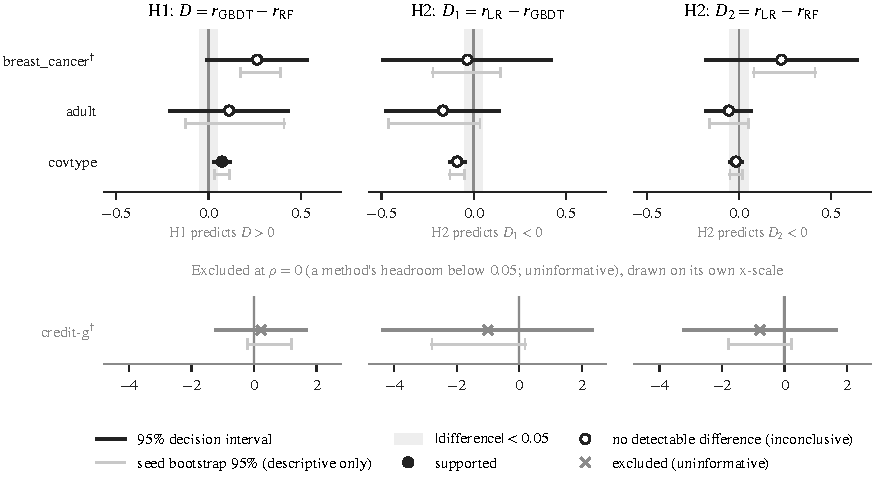
\includegraphics[width=0.92\textwidth]{figures/fig_contrasts.pdf}
\caption{Pre-specified contrasts in the share of headroom lost between $\rho=0$ and
$\rho=0.4$. Left: H1, $D = r_{\mathrm{GBDT}} - r_{\mathrm{RF}}$ (H1 predicts $D>0$). Middle
and right: H2, $D_1$ and $D_2$ (H2 predicts both $<0$). The dark line is the 95\% decision
interval: a paired $t(9)$ interval over 10 seeds, variance corrected for re-splitting on the
datasets marked $\dagger$ (\bc, \cg) and uncorrected on \ad{} and \ct. The light line below it
is the 95\% seed-bootstrap percentile interval. It is descriptive only, has no correction for
re-splitting, and never decides an outcome. The gray band marks $|D| < 0.05$. Markers give
the per-dataset outcome: filled for supported, open for no detectable difference
(inconclusive), and a cross for excluded. Under H2 the outcome is joint over $D_1$ and $D_2$.
\cg{} (excluded) is drawn on its own x-scale because its intervals are several times wider.
Overall, both H1 and H2 are inconclusive.}
\label{fig:contrasts}
\end{figure}

Table~\ref{tab:h1h2} and Figure~\ref{fig:contrasts} give the tests. Table~\ref{tab:parts}
in the appendix gives the components ($A(0)$, $A(0.4)$, drop, $h$, $r$) for each method.
\begin{itemize}
  \item \textbf{\ct: supported.} GBDT loses $r = \RCtGb$ of its headroom and RF loses
  $\RCtRf$. The difference is $D = \HOneDCt$ [$\HOneDCtLo$, $\HOneDCtHi$], with
  $S = \HOneDCtS$ and half-width $\HOneDCtHalf$. The absolute drops are $\DropCtGb$ for GBDT
  and $\DropCtRf$ for RF, a difference of $\HOneDdropCt$, so the smallest meaningful
  difference is met. This is one dataset. Each seed is a 5,000-row stratified subsample of a
  581,012-row dataset. Accuracy is dominated by the two largest of the seven classes, and the
  interval is the plain one.
  \item \textbf{\bc: no detectable difference (inconclusive).} $D = \HOneDBc$
  [$\HOneDBcLo$, $\HOneDBcHi$], with $S = \HOneDBcS$ and half-width $\HOneDBcHalf$. The
  interval includes 0. With 114 test rows and re-splits of the same 569 rows, the corrected
  interval is wide. The design stated in advance that this dataset could not reach ``no
  meaningful difference''. The point estimate is not evidence for H1 under our rule.
  \item \textbf{\ad: no detectable difference (inconclusive).} $D = \HOneDAd$
  [$\HOneDAdLo$, $\HOneDAdHi$], with $S = \HOneDAdS$ and half-width $\HOneDAdHalf$.
  \item \textbf{\cg: excluded.} For description only: $D = \HOneDCg$
  [$\HOneDCgLo$, $\HOneDCgHi$].
\end{itemize}
\textbf{Overall, H1 is inconclusive.} It is supported on \HOneNSup{} and contradicted on
\HOneNCon{} of the \HOneNInf{} informative datasets. Support needs \HOneNNeed{}.

\subsection{H2: logistic regression against the trees}

H2 needs both $D_1<0$ and $D_2<0$ to be decided on a dataset. It is inconclusive on all
\HTwoNInf{} informative datasets (\HTwoNSup{} supported, \HTwoNCon{} contradicted).
\begin{itemize}
  \item \textbf{\ct.} LR loses less of its headroom than GBDT: $D_1 = \HTwoDOneCt$
  [$\HTwoDOneCtLo$, $\HTwoDOneCtHi$], with $S = \HTwoDOneCtS$ and half-width
  $\HTwoDOneCtHalf$. LR and RF are not separable: $D_2 = \HTwoDTwoCt$
  [$\HTwoDTwoCtLo$, $\HTwoDTwoCtHi$], with $S = \HTwoDTwoCtS$ and half-width
  $\HTwoDTwoCtHalf$. The joint outcome is no detectable difference (inconclusive). LR also
  starts from a lower accuracy on this dataset ($A(0) = \AccCtLrZero$ against $\AccCtGbZero$
  for GBDT).
  \item \textbf{\ad.} $D_1 = \HTwoDOneAd$ [$\HTwoDOneAdLo$, $\HTwoDOneAdHi$] ($S =
  \HTwoDOneAdS$, half-width $\HTwoDOneAdHalf$). $D_2 = \HTwoDTwoAd$ [$\HTwoDTwoAdLo$,
  $\HTwoDTwoAdHi$] ($S = \HTwoDTwoAdS$, half-width $\HTwoDTwoAdHalf$). The outcome is no
  detectable difference (inconclusive).
  \item \textbf{\bc.} $D_1 = \HTwoDOneBc$ [$\HTwoDOneBcLo$, $\HTwoDOneBcHi$] ($S =
  \HTwoDOneBcS$, half-width $\HTwoDOneBcHalf$). $D_2 = \HTwoDTwoBc$ [$\HTwoDTwoBcLo$,
  $\HTwoDTwoBcHi$] ($S = \HTwoDTwoBcS$, half-width $\HTwoDTwoBcHalf$). The point estimate of
  $D_2$ has the sign opposite to H2's prediction: LR's $r$ is $\RBcLr$ and RF's is $\RBcRf$.
  The interval includes 0, so this is no detectable difference (inconclusive), not a
  difference.
\end{itemize}
\textbf{Overall, H2 is inconclusive.}

\subsection{The excluded dataset}

\cg{} is reported for description only. At $\rho=0.4$ all three methods fall below the
majority rate $m = \MajCg$: $A(0.4)$ is $\AccCgLrFour$ for LR, $\AccCgRfFour$ for RF and
$\AccCgGbFour$ for GBDT. Every $r$ is therefore above 1 ($\RCgLr$, $\RCgRf$, $\RCgGb$). This is
the floor case the design anticipated: with headrooms of $\HeadCgLr$ (LR), $\HeadCgRf$ (RF)
and $\HeadCgGb$ (GBDT), the measure divides by a
quantity close to the test-set noise. It is why the exclusion rule exists. No \cg{} value
enters any count.

% ---------------------------------------------------------------------------
\section{Ablations}
\label{sec:ablations}

\begin{table}[!htbp]
\centering
\resizebox{\textwidth}{!}{% Generated by code/tab_ablations.py from logged runs. Do not edit by hand; rerun the script.
% Needs \usepackage{booktabs,array} and % Generated by `crew.py numbers` from claims.jsonl. Do not edit by hand.
% Each macro is a number taken from a logged run; see claims.jsonl.
\newcommand{\NCells}{600}  % c-n-cells
\newcommand{\NFlipFail}{0}  % c-flip-fail
\newcommand{\NConvWarnCells}{0}  % c-convwarn
\newcommand{\MajBc}{0.632}  % c-m-Bc
\newcommand{\AccBcLrZero}{0.970}  % c-acc-Bc-Lr-Zero
\newcommand{\SdBcLrZero}{0.010}  % c-sd-Bc-Lr-Zero
\newcommand{\PmsBcLrZero}{0.651}  % c-pms-Bc-Lr-Zero
\newcommand{\VnBcLrZero}{0.975}  % c-vn-Bc-Lr-Zero
\newcommand{\VcBcLrZero}{0.975}  % c-vc-Bc-Lr-Zero
\newcommand{\TnBcLrZero}{0.987}  % c-tn-Bc-Lr-Zero
\newcommand{\CBcZero}{0.276}  % c-C-Bc-Zero
\newcommand{\AccBcLrOne}{0.954}  % c-acc-Bc-Lr-One
\newcommand{\SdBcLrOne}{0.029}  % c-sd-Bc-Lr-One
\newcommand{\PmsBcLrOne}{0.665}  % c-pms-Bc-Lr-One
\newcommand{\VnBcLrOne}{0.875}  % c-vn-Bc-Lr-One
\newcommand{\VcBcLrOne}{0.954}  % c-vc-Bc-Lr-One
\newcommand{\TnBcLrOne}{0.875}  % c-tn-Bc-Lr-One
\newcommand{\CBcOne}{0.104}  % c-C-Bc-One
\newcommand{\AccBcLrTwo}{0.949}  % c-acc-Bc-Lr-Two
\newcommand{\SdBcLrTwo}{0.020}  % c-sd-Bc-Lr-Two
\newcommand{\PmsBcLrTwo}{0.667}  % c-pms-Bc-Lr-Two
\newcommand{\VnBcLrTwo}{0.777}  % c-vn-Bc-Lr-Two
\newcommand{\VcBcLrTwo}{0.953}  % c-vc-Bc-Lr-Two
\newcommand{\TnBcLrTwo}{0.777}  % c-tn-Bc-Lr-Two
\newcommand{\CBcTwo}{0.0492}  % c-C-Bc-Two
\newcommand{\AccBcLrThree}{0.907}  % c-acc-Bc-Lr-Three
\newcommand{\SdBcLrThree}{0.027}  % c-sd-Bc-Lr-Three
\newcommand{\PmsBcLrThree}{0.672}  % c-pms-Bc-Lr-Three
\newcommand{\VnBcLrThree}{0.689}  % c-vn-Bc-Lr-Three
\newcommand{\VcBcLrThree}{0.909}  % c-vc-Bc-Lr-Three
\newcommand{\TnBcLrThree}{0.684}  % c-tn-Bc-Lr-Three
\newcommand{\CBcThree}{0.051}  % c-C-Bc-Three
\newcommand{\AccBcLrFour}{0.781}  % c-acc-Bc-Lr-Four
\newcommand{\SdBcLrFour}{0.098}  % c-sd-Bc-Lr-Four
\newcommand{\PmsBcLrFour}{0.670}  % c-pms-Bc-Lr-Four
\newcommand{\VnBcLrFour}{0.597}  % c-vn-Bc-Lr-Four
\newcommand{\VcBcLrFour}{0.764}  % c-vc-Bc-Lr-Four
\newcommand{\TnBcLrFour}{0.593}  % c-tn-Bc-Lr-Four
\newcommand{\CBcFour}{0.0428}  % c-C-Bc-Four
\newcommand{\AccBcRfZero}{0.951}  % c-acc-Bc-Rf-Zero
\newcommand{\SdBcRfZero}{0.032}  % c-sd-Bc-Rf-Zero
\newcommand{\PmsBcRfZero}{0.633}  % c-pms-Bc-Rf-Zero
\newcommand{\VnBcRfZero}{0.961}  % c-vn-Bc-Rf-Zero
\newcommand{\VcBcRfZero}{0.961}  % c-vc-Bc-Rf-Zero
\newcommand{\TnBcRfZero}{0.988}  % c-tn-Bc-Rf-Zero
\newcommand{\MslBcZero}{2.5}  % c-msl-Bc-Zero
\newcommand{\MfBcZero}{0.24}  % c-mf-Bc-Zero
\newcommand{\AccBcRfOne}{0.948}  % c-acc-Bc-Rf-One
\newcommand{\SdBcRfOne}{0.027}  % c-sd-Bc-Rf-One
\newcommand{\PmsBcRfOne}{0.632}  % c-pms-Bc-Rf-One
\newcommand{\VnBcRfOne}{0.877}  % c-vn-Bc-Rf-One
\newcommand{\VcBcRfOne}{0.958}  % c-vc-Bc-Rf-One
\newcommand{\TnBcRfOne}{0.921}  % c-tn-Bc-Rf-One
\newcommand{\MslBcOne}{3}  % c-msl-Bc-One
\newcommand{\MfBcOne}{0.40}  % c-mf-Bc-One
\newcommand{\AccBcRfTwo}{0.943}  % c-acc-Bc-Rf-Two
\newcommand{\SdBcRfTwo}{0.033}  % c-sd-Bc-Rf-Two
\newcommand{\PmsBcRfTwo}{0.627}  % c-pms-Bc-Rf-Two
\newcommand{\VnBcRfTwo}{0.792}  % c-vn-Bc-Rf-Two
\newcommand{\VcBcRfTwo}{0.954}  % c-vc-Bc-Rf-Two
\newcommand{\TnBcRfTwo}{0.876}  % c-tn-Bc-Rf-Two
\newcommand{\MslBcTwo}{6.5}  % c-msl-Bc-Two
\newcommand{\MfBcTwo}{0.20}  % c-mf-Bc-Two
\newcommand{\AccBcRfThree}{0.922}  % c-acc-Bc-Rf-Three
\newcommand{\SdBcRfThree}{0.026}  % c-sd-Bc-Rf-Three
\newcommand{\PmsBcRfThree}{0.636}  % c-pms-Bc-Rf-Three
\newcommand{\VnBcRfThree}{0.704}  % c-vn-Bc-Rf-Three
\newcommand{\VcBcRfThree}{0.923}  % c-vc-Bc-Rf-Three
\newcommand{\TnBcRfThree}{0.764}  % c-tn-Bc-Rf-Three
\newcommand{\MslBcThree}{15}  % c-msl-Bc-Three
\newcommand{\MfBcThree}{0.49}  % c-mf-Bc-Three
\newcommand{\AccBcRfFour}{0.846}  % c-acc-Bc-Rf-Four
\newcommand{\SdBcRfFour}{0.074}  % c-sd-Bc-Rf-Four
\newcommand{\PmsBcRfFour}{0.581}  % c-pms-Bc-Rf-Four
\newcommand{\VnBcRfFour}{0.596}  % c-vn-Bc-Rf-Four
\newcommand{\VcBcRfFour}{0.834}  % c-vc-Bc-Rf-Four
\newcommand{\TnBcRfFour}{0.755}  % c-tn-Bc-Rf-Four
\newcommand{\MslBcFour}{19.5}  % c-msl-Bc-Four
\newcommand{\MfBcFour}{0.38}  % c-mf-Bc-Four
\newcommand{\AccBcGbZero}{0.954}  % c-acc-Bc-Gb-Zero
\newcommand{\SdBcGbZero}{0.031}  % c-sd-Bc-Gb-Zero
\newcommand{\PmsBcGbZero}{0.632}  % c-pms-Bc-Gb-Zero
\newcommand{\VnBcGbZero}{0.975}  % c-vn-Bc-Gb-Zero
\newcommand{\VcBcGbZero}{0.975}  % c-vc-Bc-Gb-Zero
\newcommand{\TnBcGbZero}{1.000}  % c-tn-Bc-Gb-Zero
\newcommand{\LrateBcZero}{0.057}  % c-lrate-Bc-Zero
\newcommand{\IterBcZero}{167}  % c-iter-Bc-Zero
\newcommand{\AccBcGbOne}{0.942}  % c-acc-Bc-Gb-One
\newcommand{\SdBcGbOne}{0.033}  % c-sd-Bc-Gb-One
\newcommand{\PmsBcGbOne}{0.625}  % c-pms-Bc-Gb-One
\newcommand{\VnBcGbOne}{0.882}  % c-vn-Bc-Gb-One
\newcommand{\VcBcGbOne}{0.958}  % c-vc-Bc-Gb-One
\newcommand{\TnBcGbOne}{0.964}  % c-tn-Bc-Gb-One
\newcommand{\LrateBcOne}{0.0728}  % c-lrate-Bc-One
\newcommand{\IterBcOne}{62}  % c-iter-Bc-One
\newcommand{\AccBcGbTwo}{0.927}  % c-acc-Bc-Gb-Two
\newcommand{\SdBcGbTwo}{0.044}  % c-sd-Bc-Gb-Two
\newcommand{\PmsBcGbTwo}{0.625}  % c-pms-Bc-Gb-Two
\newcommand{\VnBcGbTwo}{0.782}  % c-vn-Bc-Gb-Two
\newcommand{\VcBcGbTwo}{0.939}  % c-vc-Bc-Gb-Two
\newcommand{\TnBcGbTwo}{0.889}  % c-tn-Bc-Gb-Two
\newcommand{\LrateBcTwo}{0.0743}  % c-lrate-Bc-Two
\newcommand{\IterBcTwo}{54}  % c-iter-Bc-Two
\newcommand{\AccBcGbThree}{0.911}  % c-acc-Bc-Gb-Three
\newcommand{\SdBcGbThree}{0.045}  % c-sd-Bc-Gb-Three
\newcommand{\PmsBcGbThree}{0.629}  % c-pms-Bc-Gb-Three
\newcommand{\VnBcGbThree}{0.698}  % c-vn-Bc-Gb-Three
\newcommand{\VcBcGbThree}{0.918}  % c-vc-Bc-Gb-Three
\newcommand{\TnBcGbThree}{0.752}  % c-tn-Bc-Gb-Three
\newcommand{\LrateBcThree}{0.0233}  % c-lrate-Bc-Three
\newcommand{\IterBcThree}{82}  % c-iter-Bc-Three
\newcommand{\AccBcGbFour}{0.762}  % c-acc-Bc-Gb-Four
\newcommand{\SdBcGbFour}{0.079}  % c-sd-Bc-Gb-Four
\newcommand{\PmsBcGbFour}{0.568}  % c-pms-Bc-Gb-Four
\newcommand{\VnBcGbFour}{0.604}  % c-vn-Bc-Gb-Four
\newcommand{\VcBcGbFour}{0.756}  % c-vc-Bc-Gb-Four
\newcommand{\TnBcGbFour}{0.800}  % c-tn-Bc-Gb-Four
\newcommand{\LrateBcFour}{0.0717}  % c-lrate-Bc-Four
\newcommand{\IterBcFour}{31}  % c-iter-Bc-Four
\newcommand{\MajCg}{0.700}  % c-m-Cg
\newcommand{\AccCgLrZero}{0.750}  % c-acc-Cg-Lr-Zero
\newcommand{\SdCgLrZero}{0.018}  % c-sd-Cg-Lr-Zero
\newcommand{\PmsCgLrZero}{0.795}  % c-pms-Cg-Lr-Zero
\newcommand{\VnCgLrZero}{0.762}  % c-vn-Cg-Lr-Zero
\newcommand{\VcCgLrZero}{0.762}  % c-vc-Cg-Lr-Zero
\newcommand{\TnCgLrZero}{0.788}  % c-tn-Cg-Lr-Zero
\newcommand{\CCgZero}{0.272}  % c-C-Cg-Zero
\newcommand{\AccCgLrOne}{0.741}  % c-acc-Cg-Lr-One
\newcommand{\SdCgLrOne}{0.016}  % c-sd-Cg-Lr-One
\newcommand{\PmsCgLrOne}{0.793}  % c-pms-Cg-Lr-One
\newcommand{\VnCgLrOne}{0.718}  % c-vn-Cg-Lr-One
\newcommand{\VcCgLrOne}{0.758}  % c-vc-Cg-Lr-One
\newcommand{\TnCgLrOne}{0.739}  % c-tn-Cg-Lr-One
\newcommand{\CCgOne}{0.255}  % c-C-Cg-One
\newcommand{\AccCgLrTwo}{0.715}  % c-acc-Cg-Lr-Two
\newcommand{\SdCgLrTwo}{0.019}  % c-sd-Cg-Lr-Two
\newcommand{\PmsCgLrTwo}{0.839}  % c-pms-Cg-Lr-Two
\newcommand{\VnCgLrTwo}{0.666}  % c-vn-Cg-Lr-Two
\newcommand{\VcCgLrTwo}{0.734}  % c-vc-Cg-Lr-Two
\newcommand{\TnCgLrTwo}{0.677}  % c-tn-Cg-Lr-Two
\newcommand{\CCgTwo}{0.0654}  % c-C-Cg-Two
\newcommand{\AccCgLrThree}{0.710}  % c-acc-Cg-Lr-Three
\newcommand{\SdCgLrThree}{0.028}  % c-sd-Cg-Lr-Three
\newcommand{\PmsCgLrThree}{0.839}  % c-pms-Cg-Lr-Three
\newcommand{\VnCgLrThree}{0.611}  % c-vn-Cg-Lr-Three
\newcommand{\VcCgLrThree}{0.718}  % c-vc-Cg-Lr-Three
\newcommand{\TnCgLrThree}{0.635}  % c-tn-Cg-Lr-Three
\newcommand{\CCgThree}{0.0336}  % c-C-Cg-Three
\newcommand{\AccCgLrFour}{0.674}  % c-acc-Cg-Lr-Four
\newcommand{\SdCgLrFour}{0.053}  % c-sd-Cg-Lr-Four
\newcommand{\PmsCgLrFour}{0.867}  % c-pms-Cg-Lr-Four
\newcommand{\VnCgLrFour}{0.576}  % c-vn-Cg-Lr-Four
\newcommand{\VcCgLrFour}{0.683}  % c-vc-Cg-Lr-Four
\newcommand{\TnCgLrFour}{0.572}  % c-tn-Cg-Lr-Four
\newcommand{\CCgFour}{0.00698}  % c-C-Cg-Four
\newcommand{\AccCgRfZero}{0.749}  % c-acc-Cg-Rf-Zero
\newcommand{\SdCgRfZero}{0.020}  % c-sd-Cg-Rf-Zero
\newcommand{\PmsCgRfZero}{0.823}  % c-pms-Cg-Rf-Zero
\newcommand{\VnCgRfZero}{0.781}  % c-vn-Cg-Rf-Zero
\newcommand{\VcCgRfZero}{0.781}  % c-vc-Cg-Rf-Zero
\newcommand{\TnCgRfZero}{0.929}  % c-tn-Cg-Rf-Zero
\newcommand{\MslCgZero}{2}  % c-msl-Cg-Zero
\newcommand{\MfCgZero}{0.26}  % c-mf-Cg-Zero
\newcommand{\AccCgRfOne}{0.739}  % c-acc-Cg-Rf-One
\newcommand{\SdCgRfOne}{0.019}  % c-sd-Cg-Rf-One
\newcommand{\PmsCgRfOne}{0.828}  % c-pms-Cg-Rf-One
\newcommand{\VnCgRfOne}{0.725}  % c-vn-Cg-Rf-One
\newcommand{\VcCgRfOne}{0.767}  % c-vc-Cg-Rf-One
\newcommand{\TnCgRfOne}{0.882}  % c-tn-Cg-Rf-One
\newcommand{\MslCgOne}{5.5}  % c-msl-Cg-One
\newcommand{\MfCgOne}{0.29}  % c-mf-Cg-One
\newcommand{\AccCgRfTwo}{0.731}  % c-acc-Cg-Rf-Two
\newcommand{\SdCgRfTwo}{0.017}  % c-sd-Cg-Rf-Two
\newcommand{\PmsCgRfTwo}{0.815}  % c-pms-Cg-Rf-Two
\newcommand{\VnCgRfTwo}{0.681}  % c-vn-Cg-Rf-Two
\newcommand{\VcCgRfTwo}{0.753}  % c-vc-Cg-Rf-Two
\newcommand{\TnCgRfTwo}{0.853}  % c-tn-Cg-Rf-Two
\newcommand{\MslCgTwo}{4.5}  % c-msl-Cg-Two
\newcommand{\MfCgTwo}{0.28}  % c-mf-Cg-Two
\newcommand{\AccCgRfThree}{0.703}  % c-acc-Cg-Rf-Three
\newcommand{\SdCgRfThree}{0.031}  % c-sd-Cg-Rf-Three
\newcommand{\PmsCgRfThree}{0.843}  % c-pms-Cg-Rf-Three
\newcommand{\VnCgRfThree}{0.629}  % c-vn-Cg-Rf-Three
\newcommand{\VcCgRfThree}{0.725}  % c-vc-Cg-Rf-Three
\newcommand{\TnCgRfThree}{0.773}  % c-tn-Cg-Rf-Three
\newcommand{\MslCgThree}{9}  % c-msl-Cg-Three
\newcommand{\MfCgThree}{0.30}  % c-mf-Cg-Three
\newcommand{\AccCgRfFour}{0.638}  % c-acc-Cg-Rf-Four
\newcommand{\SdCgRfFour}{0.047}  % c-sd-Cg-Rf-Four
\newcommand{\PmsCgRfFour}{0.728}  % c-pms-Cg-Rf-Four
\newcommand{\VnCgRfFour}{0.585}  % c-vn-Cg-Rf-Four
\newcommand{\VcCgRfFour}{0.661}  % c-vc-Cg-Rf-Four
\newcommand{\TnCgRfFour}{0.732}  % c-tn-Cg-Rf-Four
\newcommand{\MslCgFour}{15.5}  % c-msl-Cg-Four
\newcommand{\MfCgFour}{0.32}  % c-mf-Cg-Four
\newcommand{\AccCgGbZero}{0.735}  % c-acc-Cg-Gb-Zero
\newcommand{\SdCgGbZero}{0.016}  % c-sd-Cg-Gb-Zero
\newcommand{\PmsCgGbZero}{0.791}  % c-pms-Cg-Gb-Zero
\newcommand{\VnCgGbZero}{0.783}  % c-vn-Cg-Gb-Zero
\newcommand{\VcCgGbZero}{0.783}  % c-vc-Cg-Gb-Zero
\newcommand{\TnCgGbZero}{0.932}  % c-tn-Cg-Gb-Zero
\newcommand{\LrateCgZero}{0.158}  % c-lrate-Cg-Zero
\newcommand{\IterCgZero}{56}  % c-iter-Cg-Zero
\newcommand{\AccCgGbOne}{0.729}  % c-acc-Cg-Gb-One
\newcommand{\SdCgGbOne}{0.026}  % c-sd-Cg-Gb-One
\newcommand{\PmsCgGbOne}{0.779}  % c-pms-Cg-Gb-One
\newcommand{\VnCgGbOne}{0.730}  % c-vn-Cg-Gb-One
\newcommand{\VcCgGbOne}{0.764}  % c-vc-Cg-Gb-One
\newcommand{\TnCgGbOne}{0.856}  % c-tn-Cg-Gb-One
\newcommand{\LrateCgOne}{0.044}  % c-lrate-Cg-One
\newcommand{\IterCgOne}{76}  % c-iter-Cg-One
\newcommand{\AccCgGbTwo}{0.714}  % c-acc-Cg-Gb-Two
\newcommand{\SdCgGbTwo}{0.018}  % c-sd-Cg-Gb-Two
\newcommand{\PmsCgGbTwo}{0.797}  % c-pms-Cg-Gb-Two
\newcommand{\VnCgGbTwo}{0.684}  % c-vn-Cg-Gb-Two
\newcommand{\VcCgGbTwo}{0.742}  % c-vc-Cg-Gb-Two
\newcommand{\TnCgGbTwo}{0.793}  % c-tn-Cg-Gb-Two
\newcommand{\LrateCgTwo}{0.0254}  % c-lrate-Cg-Two
\newcommand{\IterCgTwo}{102}  % c-iter-Cg-Two
\newcommand{\AccCgGbThree}{0.692}  % c-acc-Cg-Gb-Three
\newcommand{\SdCgGbThree}{0.027}  % c-sd-Cg-Gb-Three
\newcommand{\PmsCgGbThree}{0.793}  % c-pms-Cg-Gb-Three
\newcommand{\VnCgGbThree}{0.626}  % c-vn-Cg-Gb-Three
\newcommand{\VcCgGbThree}{0.705}  % c-vc-Cg-Gb-Three
\newcommand{\TnCgGbThree}{0.728}  % c-tn-Cg-Gb-Three
\newcommand{\LrateCgThree}{0.0316}  % c-lrate-Cg-Three
\newcommand{\IterCgThree}{53}  % c-iter-Cg-Three
\newcommand{\AccCgGbFour}{0.647}  % c-acc-Cg-Gb-Four
\newcommand{\SdCgGbFour}{0.046}  % c-sd-Cg-Gb-Four
\newcommand{\PmsCgGbFour}{0.783}  % c-pms-Cg-Gb-Four
\newcommand{\VnCgGbFour}{0.581}  % c-vn-Cg-Gb-Four
\newcommand{\VcCgGbFour}{0.651}  % c-vc-Cg-Gb-Four
\newcommand{\TnCgGbFour}{0.667}  % c-tn-Cg-Gb-Four
\newcommand{\LrateCgFour}{0.0251}  % c-lrate-Cg-Four
\newcommand{\IterCgFour}{29}  % c-iter-Cg-Four
\newcommand{\MajAd}{0.761}  % c-m-Ad
\newcommand{\AccAdLrZero}{0.843}  % c-acc-Ad-Lr-Zero
\newcommand{\SdAdLrZero}{0.012}  % c-sd-Ad-Lr-Zero
\newcommand{\PmsAdLrZero}{0.812}  % c-pms-Ad-Lr-Zero
\newcommand{\VnAdLrZero}{0.849}  % c-vn-Ad-Lr-Zero
\newcommand{\VcAdLrZero}{0.849}  % c-vc-Ad-Lr-Zero
\newcommand{\TnAdLrZero}{0.855}  % c-tn-Ad-Lr-Zero
\newcommand{\CAdZero}{0.38}  % c-C-Ad-Zero
\newcommand{\AccAdLrOne}{0.838}  % c-acc-Ad-Lr-One
\newcommand{\SdAdLrOne}{0.010}  % c-sd-Ad-Lr-One
\newcommand{\PmsAdLrOne}{0.822}  % c-pms-Ad-Lr-One
\newcommand{\VnAdLrOne}{0.776}  % c-vn-Ad-Lr-One
\newcommand{\VcAdLrOne}{0.844}  % c-vc-Ad-Lr-One
\newcommand{\TnAdLrOne}{0.780}  % c-tn-Ad-Lr-One
\newcommand{\CAdOne}{0.182}  % c-C-Ad-One
\newcommand{\AccAdLrTwo}{0.830}  % c-acc-Ad-Lr-Two
\newcommand{\SdAdLrTwo}{0.009}  % c-sd-Ad-Lr-Two
\newcommand{\PmsAdLrTwo}{0.848}  % c-pms-Ad-Lr-Two
\newcommand{\VnAdLrTwo}{0.703}  % c-vn-Ad-Lr-Two
\newcommand{\VcAdLrTwo}{0.833}  % c-vc-Ad-Lr-Two
\newcommand{\TnAdLrTwo}{0.703}  % c-tn-Ad-Lr-Two
\newcommand{\CAdTwo}{0.0195}  % c-C-Ad-Two
\newcommand{\AccAdLrThree}{0.821}  % c-acc-Ad-Lr-Three
\newcommand{\SdAdLrThree}{0.009}  % c-sd-Ad-Lr-Three
\newcommand{\PmsAdLrThree}{0.847}  % c-pms-Ad-Lr-Three
\newcommand{\VnAdLrThree}{0.637}  % c-vn-Ad-Lr-Three
\newcommand{\VcAdLrThree}{0.823}  % c-vc-Ad-Lr-Three
\newcommand{\TnAdLrThree}{0.637}  % c-tn-Ad-Lr-Three
\newcommand{\CAdThree}{0.0202}  % c-C-Ad-Three
\newcommand{\AccAdLrFour}{0.797}  % c-acc-Ad-Lr-Four
\newcommand{\SdAdLrFour}{0.015}  % c-sd-Ad-Lr-Four
\newcommand{\PmsAdLrFour}{0.833}  % c-pms-Ad-Lr-Four
\newcommand{\VnAdLrFour}{0.569}  % c-vn-Ad-Lr-Four
\newcommand{\VcAdLrFour}{0.804}  % c-vc-Ad-Lr-Four
\newcommand{\TnAdLrFour}{0.572}  % c-tn-Ad-Lr-Four
\newcommand{\CAdFour}{0.00584}  % c-C-Ad-Four
\newcommand{\AccAdRfZero}{0.847}  % c-acc-Ad-Rf-Zero
\newcommand{\SdAdRfZero}{0.010}  % c-sd-Ad-Rf-Zero
\newcommand{\PmsAdRfZero}{0.814}  % c-pms-Ad-Rf-Zero
\newcommand{\VnAdRfZero}{0.859}  % c-vn-Ad-Rf-Zero
\newcommand{\VcAdRfZero}{0.859}  % c-vc-Ad-Rf-Zero
\newcommand{\TnAdRfZero}{0.911}  % c-tn-Ad-Rf-Zero
\newcommand{\MslAdZero}{3}  % c-msl-Ad-Zero
\newcommand{\MfAdZero}{0.20}  % c-mf-Ad-Zero
\newcommand{\AccAdRfOne}{0.845}  % c-acc-Ad-Rf-One
\newcommand{\SdAdRfOne}{0.012}  % c-sd-Ad-Rf-One
\newcommand{\PmsAdRfOne}{0.812}  % c-pms-Ad-Rf-One
\newcommand{\VnAdRfOne}{0.788}  % c-vn-Ad-Rf-One
\newcommand{\VcAdRfOne}{0.855}  % c-vc-Ad-Rf-One
\newcommand{\TnAdRfOne}{0.829}  % c-tn-Ad-Rf-One
\newcommand{\MslAdOne}{3.5}  % c-msl-Ad-One
\newcommand{\MfAdOne}{0.22}  % c-mf-Ad-One
\newcommand{\AccAdRfTwo}{0.836}  % c-acc-Ad-Rf-Two
\newcommand{\SdAdRfTwo}{0.006}  % c-sd-Ad-Rf-Two
\newcommand{\PmsAdRfTwo}{0.823}  % c-pms-Ad-Rf-Two
\newcommand{\VnAdRfTwo}{0.714}  % c-vn-Ad-Rf-Two
\newcommand{\VcAdRfTwo}{0.847}  % c-vc-Ad-Rf-Two
\newcommand{\TnAdRfTwo}{0.760}  % c-tn-Ad-Rf-Two
\newcommand{\MslAdTwo}{2.5}  % c-msl-Ad-Two
\newcommand{\MfAdTwo}{0.11}  % c-mf-Ad-Two
\newcommand{\AccAdRfThree}{0.830}  % c-acc-Ad-Rf-Three
\newcommand{\SdAdRfThree}{0.016}  % c-sd-Ad-Rf-Three
\newcommand{\PmsAdRfThree}{0.809}  % c-pms-Ad-Rf-Three
\newcommand{\VnAdRfThree}{0.644}  % c-vn-Ad-Rf-Three
\newcommand{\VcAdRfThree}{0.834}  % c-vc-Ad-Rf-Three
\newcommand{\TnAdRfThree}{0.715}  % c-tn-Ad-Rf-Three
\newcommand{\MslAdThree}{11}  % c-msl-Ad-Three
\newcommand{\MfAdThree}{0.13}  % c-mf-Ad-Three
\newcommand{\AccAdRfFour}{0.794}  % c-acc-Ad-Rf-Four
\newcommand{\SdAdRfFour}{0.021}  % c-sd-Ad-Rf-Four
\newcommand{\PmsAdRfFour}{0.776}  % c-pms-Ad-Rf-Four
\newcommand{\VnAdRfFour}{0.571}  % c-vn-Ad-Rf-Four
\newcommand{\VcAdRfFour}{0.804}  % c-vc-Ad-Rf-Four
\newcommand{\TnAdRfFour}{0.646}  % c-tn-Ad-Rf-Four
\newcommand{\MslAdFour}{23}  % c-msl-Ad-Four
\newcommand{\MfAdFour}{0.28}  % c-mf-Ad-Four
\newcommand{\AccAdGbZero}{0.852}  % c-acc-Ad-Gb-Zero
\newcommand{\SdAdGbZero}{0.009}  % c-sd-Ad-Gb-Zero
\newcommand{\PmsAdGbZero}{0.803}  % c-pms-Ad-Gb-Zero
\newcommand{\VnAdGbZero}{0.866}  % c-vn-Ad-Gb-Zero
\newcommand{\VcAdGbZero}{0.866}  % c-vc-Ad-Gb-Zero
\newcommand{\TnAdGbZero}{0.907}  % c-tn-Ad-Gb-Zero
\newcommand{\LrateAdZero}{0.109}  % c-lrate-Ad-Zero
\newcommand{\IterAdZero}{94}  % c-iter-Ad-Zero
\newcommand{\AccAdGbOne}{0.850}  % c-acc-Ad-Gb-One
\newcommand{\SdAdGbOne}{0.007}  % c-sd-Ad-Gb-One
\newcommand{\PmsAdGbOne}{0.821}  % c-pms-Ad-Gb-One
\newcommand{\VnAdGbOne}{0.792}  % c-vn-Ad-Gb-One
\newcommand{\VcAdGbOne}{0.861}  % c-vc-Ad-Gb-One
\newcommand{\TnAdGbOne}{0.813}  % c-tn-Ad-Gb-One
\newcommand{\LrateAdOne}{0.0201}  % c-lrate-Ad-One
\newcommand{\IterAdOne}{173}  % c-iter-Ad-One
\newcommand{\AccAdGbTwo}{0.840}  % c-acc-Ad-Gb-Two
\newcommand{\SdAdGbTwo}{0.008}  % c-sd-Ad-Gb-Two
\newcommand{\PmsAdGbTwo}{0.822}  % c-pms-Ad-Gb-Two
\newcommand{\VnAdGbTwo}{0.717}  % c-vn-Ad-Gb-Two
\newcommand{\VcAdGbTwo}{0.853}  % c-vc-Ad-Gb-Two
\newcommand{\TnAdGbTwo}{0.749}  % c-tn-Ad-Gb-Two
\newcommand{\LrateAdTwo}{0.0229}  % c-lrate-Ad-Two
\newcommand{\IterAdTwo}{120}  % c-iter-Ad-Two
\newcommand{\AccAdGbThree}{0.829}  % c-acc-Ad-Gb-Three
\newcommand{\SdAdGbThree}{0.014}  % c-sd-Ad-Gb-Three
\newcommand{\PmsAdGbThree}{0.829}  % c-pms-Ad-Gb-Three
\newcommand{\VnAdGbThree}{0.646}  % c-vn-Ad-Gb-Three
\newcommand{\VcAdGbThree}{0.838}  % c-vc-Ad-Gb-Three
\newcommand{\TnAdGbThree}{0.682}  % c-tn-Ad-Gb-Three
\newcommand{\LrateAdThree}{0.0257}  % c-lrate-Ad-Three
\newcommand{\IterAdThree}{86}  % c-iter-Ad-Three
\newcommand{\AccAdGbFour}{0.786}  % c-acc-Ad-Gb-Four
\newcommand{\SdAdGbFour}{0.040}  % c-sd-Ad-Gb-Four
\newcommand{\PmsAdGbFour}{0.842}  % c-pms-Ad-Gb-Four
\newcommand{\VnAdGbFour}{0.571}  % c-vn-Ad-Gb-Four
\newcommand{\VcAdGbFour}{0.795}  % c-vc-Ad-Gb-Four
\newcommand{\TnAdGbFour}{0.606}  % c-tn-Ad-Gb-Four
\newcommand{\LrateAdFour}{0.0169}  % c-lrate-Ad-Four
\newcommand{\IterAdFour}{64}  % c-iter-Ad-Four
\newcommand{\MajCt}{0.488}  % c-m-Ct
\newcommand{\AccCtLrZero}{0.715}  % c-acc-Ct-Lr-Zero
\newcommand{\SdCtLrZero}{0.011}  % c-sd-Ct-Lr-Zero
\newcommand{\PmsCtLrZero}{0.526}  % c-pms-Ct-Lr-Zero
\newcommand{\VnCtLrZero}{0.718}  % c-vn-Ct-Lr-Zero
\newcommand{\VcCtLrZero}{0.718}  % c-vc-Ct-Lr-Zero
\newcommand{\TnCtLrZero}{0.736}  % c-tn-Ct-Lr-Zero
\newcommand{\CCtZero}{2.25}  % c-C-Ct-Zero
\newcommand{\AccCtLrOne}{0.704}  % c-acc-Ct-Lr-One
\newcommand{\SdCtLrOne}{0.011}  % c-sd-Ct-Lr-One
\newcommand{\PmsCtLrOne}{0.540}  % c-pms-Ct-Lr-One
\newcommand{\VnCtLrOne}{0.645}  % c-vn-Ct-Lr-One
\newcommand{\VcCtLrOne}{0.710}  % c-vc-Ct-Lr-One
\newcommand{\TnCtLrOne}{0.656}  % c-tn-Ct-Lr-One
\newcommand{\CCtOne}{2.75}  % c-C-Ct-One
\newcommand{\AccCtLrTwo}{0.697}  % c-acc-Ct-Lr-Two
\newcommand{\SdCtLrTwo}{0.016}  % c-sd-Ct-Lr-Two
\newcommand{\PmsCtLrTwo}{0.544}  % c-pms-Ct-Lr-Two
\newcommand{\VnCtLrTwo}{0.576}  % c-vn-Ct-Lr-Two
\newcommand{\VcCtLrTwo}{0.703}  % c-vc-Ct-Lr-Two
\newcommand{\TnCtLrTwo}{0.586}  % c-tn-Ct-Lr-Two
\newcommand{\CCtTwo}{0.336}  % c-C-Ct-Two
\newcommand{\AccCtLrThree}{0.696}  % c-acc-Ct-Lr-Three
\newcommand{\SdCtLrThree}{0.015}  % c-sd-Ct-Lr-Three
\newcommand{\PmsCtLrThree}{0.550}  % c-pms-Ct-Lr-Three
\newcommand{\VnCtLrThree}{0.509}  % c-vn-Ct-Lr-Three
\newcommand{\VcCtLrThree}{0.697}  % c-vc-Ct-Lr-Three
\newcommand{\TnCtLrThree}{0.515}  % c-tn-Ct-Lr-Three
\newcommand{\CCtThree}{4.04}  % c-C-Ct-Three
\newcommand{\AccCtLrFour}{0.689}  % c-acc-Ct-Lr-Four
\newcommand{\SdCtLrFour}{0.014}  % c-sd-Ct-Lr-Four
\newcommand{\PmsCtLrFour}{0.555}  % c-pms-Ct-Lr-Four
\newcommand{\VnCtLrFour}{0.436}  % c-vn-Ct-Lr-Four
\newcommand{\VcCtLrFour}{0.688}  % c-vc-Ct-Lr-Four
\newcommand{\TnCtLrFour}{0.450}  % c-tn-Ct-Lr-Four
\newcommand{\CCtFour}{0.62}  % c-C-Ct-Four
\newcommand{\AccCtRfZero}{0.755}  % c-acc-Ct-Rf-Zero
\newcommand{\SdCtRfZero}{0.014}  % c-sd-Ct-Rf-Zero
\newcommand{\PmsCtRfZero}{0.523}  % c-pms-Ct-Rf-Zero
\newcommand{\VnCtRfZero}{0.760}  % c-vn-Ct-Rf-Zero
\newcommand{\VcCtRfZero}{0.760}  % c-vc-Ct-Rf-Zero
\newcommand{\TnCtRfZero}{0.992}  % c-tn-Ct-Rf-Zero
\newcommand{\MslCtZero}{1}  % c-msl-Ct-Zero
\newcommand{\MfCtZero}{0.45}  % c-mf-Ct-Zero
\newcommand{\AccCtRfOne}{0.753}  % c-acc-Ct-Rf-One
\newcommand{\SdCtRfOne}{0.012}  % c-sd-Ct-Rf-One
\newcommand{\PmsCtRfOne}{0.529}  % c-pms-Ct-Rf-One
\newcommand{\VnCtRfOne}{0.687}  % c-vn-Ct-Rf-One
\newcommand{\VcCtRfOne}{0.759}  % c-vc-Ct-Rf-One
\newcommand{\TnCtRfOne}{0.976}  % c-tn-Ct-Rf-One
\newcommand{\MslCtOne}{1}  % c-msl-Ct-One
\newcommand{\MfCtOne}{0.42}  % c-mf-Ct-One
\newcommand{\AccCtRfTwo}{0.744}  % c-acc-Ct-Rf-Two
\newcommand{\SdCtRfTwo}{0.012}  % c-sd-Ct-Rf-Two
\newcommand{\PmsCtRfTwo}{0.534}  % c-pms-Ct-Rf-Two
\newcommand{\VnCtRfTwo}{0.609}  % c-vn-Ct-Rf-Two
\newcommand{\VcCtRfTwo}{0.754}  % c-vc-Ct-Rf-Two
\newcommand{\TnCtRfTwo}{0.960}  % c-tn-Ct-Rf-Two
\newcommand{\MslCtTwo}{1.5}  % c-msl-Ct-Two
\newcommand{\MfCtTwo}{0.37}  % c-mf-Ct-Two
\newcommand{\AccCtRfThree}{0.730}  % c-acc-Ct-Rf-Three
\newcommand{\SdCtRfThree}{0.016}  % c-sd-Ct-Rf-Three
\newcommand{\PmsCtRfThree}{0.531}  % c-pms-Ct-Rf-Three
\newcommand{\VnCtRfThree}{0.533}  % c-vn-Ct-Rf-Three
\newcommand{\VcCtRfThree}{0.739}  % c-vc-Ct-Rf-Three
\newcommand{\TnCtRfThree}{0.758}  % c-tn-Ct-Rf-Three
\newcommand{\MslCtThree}{3.5}  % c-msl-Ct-Three
\newcommand{\MfCtThree}{0.37}  % c-mf-Ct-Three
\newcommand{\AccCtRfFour}{0.719}  % c-acc-Ct-Rf-Four
\newcommand{\SdCtRfFour}{0.011}  % c-sd-Ct-Rf-Four
\newcommand{\PmsCtRfFour}{0.539}  % c-pms-Ct-Rf-Four
\newcommand{\VnCtRfFour}{0.454}  % c-vn-Ct-Rf-Four
\newcommand{\VcCtRfFour}{0.726}  % c-vc-Ct-Rf-Four
\newcommand{\TnCtRfFour}{0.774}  % c-tn-Ct-Rf-Four
\newcommand{\MslCtFour}{2.5}  % c-msl-Ct-Four
\newcommand{\MfCtFour}{0.36}  % c-mf-Ct-Four
\newcommand{\AccCtGbZero}{0.755}  % c-acc-Ct-Gb-Zero
\newcommand{\SdCtGbZero}{0.012}  % c-sd-Ct-Gb-Zero
\newcommand{\PmsCtGbZero}{0.525}  % c-pms-Ct-Gb-Zero
\newcommand{\VnCtGbZero}{0.755}  % c-vn-Ct-Gb-Zero
\newcommand{\VcCtGbZero}{0.755}  % c-vc-Ct-Gb-Zero
\newcommand{\TnCtGbZero}{0.962}  % c-tn-Ct-Gb-Zero
\newcommand{\LrateCtZero}{0.0393}  % c-lrate-Ct-Zero
\newcommand{\IterCtZero}{89}  % c-iter-Ct-Zero
\newcommand{\AccCtGbOne}{0.740}  % c-acc-Ct-Gb-One
\newcommand{\SdCtGbOne}{0.010}  % c-sd-Ct-Gb-One
\newcommand{\PmsCtGbOne}{0.531}  % c-pms-Ct-Gb-One
\newcommand{\VnCtGbOne}{0.677}  % c-vn-Ct-Gb-One
\newcommand{\VcCtGbOne}{0.746}  % c-vc-Ct-Gb-One
\newcommand{\TnCtGbOne}{0.939}  % c-tn-Ct-Gb-One
\newcommand{\LrateCtOne}{0.0341}  % c-lrate-Ct-One
\newcommand{\IterCtOne}{84}  % c-iter-Ct-One
\newcommand{\AccCtGbTwo}{0.726}  % c-acc-Ct-Gb-Two
\newcommand{\SdCtGbTwo}{0.012}  % c-sd-Ct-Gb-Two
\newcommand{\PmsCtGbTwo}{0.536}  % c-pms-Ct-Gb-Two
\newcommand{\VnCtGbTwo}{0.600}  % c-vn-Ct-Gb-Two
\newcommand{\VcCtGbTwo}{0.736}  % c-vc-Ct-Gb-Two
\newcommand{\TnCtGbTwo}{0.788}  % c-tn-Ct-Gb-Two
\newcommand{\LrateCtTwo}{0.0431}  % c-lrate-Ct-Two
\newcommand{\IterCtTwo}{64}  % c-iter-Ct-Two
\newcommand{\AccCtGbThree}{0.717}  % c-acc-Ct-Gb-Three
\newcommand{\SdCtGbThree}{0.014}  % c-sd-Ct-Gb-Three
\newcommand{\PmsCtGbThree}{0.535}  % c-pms-Ct-Gb-Three
\newcommand{\VnCtGbThree}{0.525}  % c-vn-Ct-Gb-Three
\newcommand{\VcCtGbThree}{0.724}  % c-vc-Ct-Gb-Three
\newcommand{\TnCtGbThree}{0.633}  % c-tn-Ct-Gb-Three
\newcommand{\LrateCtThree}{0.0603}  % c-lrate-Ct-Three
\newcommand{\IterCtThree}{56}  % c-iter-Ct-Three
\newcommand{\AccCtGbFour}{0.700}  % c-acc-Ct-Gb-Four
\newcommand{\SdCtGbFour}{0.018}  % c-sd-Ct-Gb-Four
\newcommand{\PmsCtGbFour}{0.545}  % c-pms-Ct-Gb-Four
\newcommand{\VnCtGbFour}{0.451}  % c-vn-Ct-Gb-Four
\newcommand{\VcCtGbFour}{0.710}  % c-vc-Ct-Gb-Four
\newcommand{\TnCtGbFour}{0.531}  % c-tn-Ct-Gb-Four
\newcommand{\LrateCtFour}{0.0457}  % c-lrate-Ct-Four
\newcommand{\IterCtFour}{51}  % c-iter-Ct-Four
\newcommand{\HeadBcLr}{0.339}  % c-head-Bc-Lr
\newcommand{\HeadBcRf}{0.319}  % c-head-Bc-Rf
\newcommand{\HeadBcGb}{0.322}  % c-head-Bc-Gb
\newcommand{\HeadCgLr}{0.051}  % c-head-Cg-Lr
\newcommand{\HeadCgRf}{0.049}  % c-head-Cg-Rf
\newcommand{\HeadCgGb}{0.035}  % c-head-Cg-Gb
\newcommand{\HeadAdLr}{0.082}  % c-head-Ad-Lr
\newcommand{\HeadAdRf}{0.086}  % c-head-Ad-Rf
\newcommand{\HeadAdGb}{0.091}  % c-head-Ad-Gb
\newcommand{\HeadCtLr}{0.227}  % c-head-Ct-Lr
\newcommand{\HeadCtRf}{0.267}  % c-head-Ct-Rf
\newcommand{\HeadCtGb}{0.268}  % c-head-Ct-Gb
\newcommand{\NInfHOne}{3}  % c-ninf-h1
\newcommand{\NInfHTwo}{3}  % c-ninf-h2
\newcommand{\HBcLr}{0.339}  % c-h-Bc-Lr
\newcommand{\HloBcLr}{0.323}  % c-hlo-Bc-Lr
\newcommand{\DropBcLr}{0.189}  % c-drop-Bc-Lr
\newcommand{\RBcLr}{0.560}  % c-r-Bc-Lr
\newcommand{\HBcRf}{0.319}  % c-h-Bc-Rf
\newcommand{\HloBcRf}{0.272}  % c-hlo-Bc-Rf
\newcommand{\DropBcRf}{0.105}  % c-drop-Bc-Rf
\newcommand{\RBcRf}{0.330}  % c-r-Bc-Rf
\newcommand{\HBcGb}{0.322}  % c-h-Bc-Gb
\newcommand{\HloBcGb}{0.276}  % c-hlo-Bc-Gb
\newcommand{\DropBcGb}{0.191}  % c-drop-Bc-Gb
\newcommand{\RBcGb}{0.594}  % c-r-Bc-Gb
\newcommand{\HOneDBc}{0.264}  % c-h1-Bc
\newcommand{\HOneDBcLo}{-0.014}  % c-h1-Bc-lo
\newcommand{\HOneDBcHi}{0.543}  % c-h1-Bc-hi
\newcommand{\HOneDBcS}{0.187}  % c-h1-Bc-s
\newcommand{\HOneDBcHalf}{0.279}  % c-h1-Bc-half
\newcommand{\HOneDBcBootLo}{0.173}  % c-h1-Bc-blo
\newcommand{\HOneDBcBootHi}{0.390}  % c-h1-Bc-bhi
\newcommand{\HOneDdropBc}{0.086}  % c-h1-Bc-ddrop
\newcommand{\HTwoDOneBc}{-0.034}  % c-h2-Bc-d1
\newcommand{\HTwoDOneBcLo}{-0.497}  % c-h2-Bc-d1-lo
\newcommand{\HTwoDOneBcHi}{0.428}  % c-h2-Bc-d1-hi
\newcommand{\HTwoDOneBcS}{0.310}  % c-h2-Bc-d1-s
\newcommand{\HTwoDOneBcHalf}{0.463}  % c-h2-Bc-d1-half
\newcommand{\HTwoDOneBcBootLo}{-0.221}  % c-h2-Bc-d1-blo
\newcommand{\HTwoDOneBcBootHi}{0.147}  % c-h2-Bc-d1-bhi
\newcommand{\HTwoDOneDdropBc}{-0.002}  % c-h2-Bc-d1-ddrop
\newcommand{\HTwoDTwoBc}{0.230}  % c-h2-Bc-d2
\newcommand{\HTwoDTwoBcLo}{-0.189}  % c-h2-Bc-d2-lo
\newcommand{\HTwoDTwoBcHi}{0.648}  % c-h2-Bc-d2-hi
\newcommand{\HTwoDTwoBcS}{0.281}  % c-h2-Bc-d2-s
\newcommand{\HTwoDTwoBcHalf}{0.418}  % c-h2-Bc-d2-half
\newcommand{\HTwoDTwoBcBootLo}{0.081}  % c-h2-Bc-d2-blo
\newcommand{\HTwoDTwoBcBootHi}{0.412}  % c-h2-Bc-d2-bhi
\newcommand{\HTwoDTwoDdropBc}{0.084}  % c-h2-Bc-d2-ddrop
\newcommand{\HCgLr}{0.051}  % c-h-Cg-Lr
\newcommand{\HloCgLr}{0.024}  % c-hlo-Cg-Lr
\newcommand{\DropCgLr}{0.076}  % c-drop-Cg-Lr
\newcommand{\RCgLr}{1.505}  % c-r-Cg-Lr
\newcommand{\HCgRf}{0.049}  % c-h-Cg-Rf
\newcommand{\HloCgRf}{0.019}  % c-hlo-Cg-Rf
\newcommand{\DropCgRf}{0.111}  % c-drop-Cg-Rf
\newcommand{\RCgRf}{2.278}  % c-r-Cg-Rf
\newcommand{\HCgGb}{0.035}  % c-h-Cg-Gb
\newcommand{\HloCgGb}{0.011}  % c-hlo-Cg-Gb
\newcommand{\DropCgGb}{0.088}  % c-drop-Cg-Gb
\newcommand{\RCgGb}{2.514}  % c-r-Cg-Gb
\newcommand{\HOneDCg}{0.236}  % c-h1-Cg
\newcommand{\HOneDCgLo}{-1.253}  % c-h1-Cg-lo
\newcommand{\HOneDCgHi}{1.725}  % c-h1-Cg-hi
\newcommand{\HOneDCgS}{1.000}  % c-h1-Cg-s
\newcommand{\HOneDCgHalf}{1.489}  % c-h1-Cg-half
\newcommand{\HOneDCgBootLo}{-0.218}  % c-h1-Cg-blo
\newcommand{\HOneDCgBootHi}{1.198}  % c-h1-Cg-bhi
\newcommand{\HOneDdropCg}{-0.022}  % c-h1-Cg-ddrop
\newcommand{\HTwoDOneCg}{-1.009}  % c-h2-Cg-d1
\newcommand{\HTwoDOneCgLo}{-4.392}  % c-h2-Cg-d1-lo
\newcommand{\HTwoDOneCgHi}{2.373}  % c-h2-Cg-d1-hi
\newcommand{\HTwoDOneCgS}{2.271}  % c-h2-Cg-d1-s
\newcommand{\HTwoDOneCgHalf}{3.383}  % c-h2-Cg-d1-half
\newcommand{\HTwoDOneCgBootLo}{-2.792}  % c-h2-Cg-d1-blo
\newcommand{\HTwoDOneCgBootHi}{0.187}  % c-h2-Cg-d1-bhi
\newcommand{\HTwoDOneDdropCg}{-0.012}  % c-h2-Cg-d1-ddrop
\newcommand{\HTwoDTwoCg}{-0.773}  % c-h2-Cg-d2
\newcommand{\HTwoDTwoCgLo}{-3.253}  % c-h2-Cg-d2-lo
\newcommand{\HTwoDTwoCgHi}{1.706}  % c-h2-Cg-d2-hi
\newcommand{\HTwoDTwoCgS}{1.665}  % c-h2-Cg-d2-s
\newcommand{\HTwoDTwoCgHalf}{2.479}  % c-h2-Cg-d2-half
\newcommand{\HTwoDTwoCgBootLo}{-1.788}  % c-h2-Cg-d2-blo
\newcommand{\HTwoDTwoCgBootHi}{0.228}  % c-h2-Cg-d2-bhi
\newcommand{\HTwoDTwoDdropCg}{-0.035}  % c-h2-Cg-d2-ddrop
\newcommand{\HAdLr}{0.082}  % c-h-Ad-Lr
\newcommand{\HloAdLr}{0.074}  % c-hlo-Ad-Lr
\newcommand{\DropAdLr}{0.046}  % c-drop-Ad-Lr
\newcommand{\RAdLr}{0.559}  % c-r-Ad-Lr
\newcommand{\HAdRf}{0.086}  % c-h-Ad-Rf
\newcommand{\HloAdRf}{0.078}  % c-hlo-Ad-Rf
\newcommand{\DropAdRf}{0.053}  % c-drop-Ad-Rf
\newcommand{\RAdRf}{0.614}  % c-r-Ad-Rf
\newcommand{\HAdGb}{0.091}  % c-h-Ad-Gb
\newcommand{\HloAdGb}{0.085}  % c-hlo-Ad-Gb
\newcommand{\DropAdGb}{0.066}  % c-drop-Ad-Gb
\newcommand{\RAdGb}{0.726}  % c-r-Ad-Gb
\newcommand{\HOneDAd}{0.112}  % c-h1-Ad
\newcommand{\HOneDAdLo}{-0.217}  % c-h1-Ad-lo
\newcommand{\HOneDAdHi}{0.440}  % c-h1-Ad-hi
\newcommand{\HOneDAdS}{0.459}  % c-h1-Ad-s
\newcommand{\HOneDAdHalf}{0.328}  % c-h1-Ad-half
\newcommand{\HOneDAdBootLo}{-0.123}  % c-h1-Ad-blo
\newcommand{\HOneDAdBootHi}{0.410}  % c-h1-Ad-bhi
\newcommand{\HOneDdropAd}{0.014}  % c-h1-Ad-ddrop
\newcommand{\HTwoDOneAd}{-0.167}  % c-h2-Ad-d1
\newcommand{\HTwoDOneAdLo}{-0.481}  % c-h2-Ad-d1-lo
\newcommand{\HTwoDOneAdHi}{0.147}  % c-h2-Ad-d1-hi
\newcommand{\HTwoDOneAdS}{0.439}  % c-h2-Ad-d1-s
\newcommand{\HTwoDOneAdHalf}{0.314}  % c-h2-Ad-d1-half
\newcommand{\HTwoDOneAdBootLo}{-0.461}  % c-h2-Ad-d1-blo
\newcommand{\HTwoDOneAdBootHi}{0.034}  % c-h2-Ad-d1-bhi
\newcommand{\HTwoDOneDdropAd}{-0.021}  % c-h2-Ad-d1-ddrop
\newcommand{\HTwoDTwoAd}{-0.055}  % c-h2-Ad-d2
\newcommand{\HTwoDTwoAdLo}{-0.184}  % c-h2-Ad-d2-lo
\newcommand{\HTwoDTwoAdHi}{0.073}  % c-h2-Ad-d2-hi
\newcommand{\HTwoDTwoAdS}{0.180}  % c-h2-Ad-d2-s
\newcommand{\HTwoDTwoAdHalf}{0.129}  % c-h2-Ad-d2-half
\newcommand{\HTwoDTwoAdBootLo}{-0.160}  % c-h2-Ad-d2-blo
\newcommand{\HTwoDTwoAdBootHi}{0.053}  % c-h2-Ad-d2-bhi
\newcommand{\HTwoDTwoDdropAd}{-0.007}  % c-h2-Ad-d2-ddrop
\newcommand{\HCtLr}{0.227}  % c-h-Ct-Lr
\newcommand{\HloCtLr}{0.219}  % c-hlo-Ct-Lr
\newcommand{\DropCtLr}{0.027}  % c-drop-Ct-Lr
\newcommand{\RCtLr}{0.118}  % c-r-Ct-Lr
\newcommand{\HCtRf}{0.267}  % c-h-Ct-Rf
\newcommand{\HloCtRf}{0.258}  % c-hlo-Ct-Rf
\newcommand{\DropCtRf}{0.036}  % c-drop-Ct-Rf
\newcommand{\RCtRf}{0.135}  % c-r-Ct-Rf
\newcommand{\HCtGb}{0.268}  % c-h-Ct-Gb
\newcommand{\HloCtGb}{0.259}  % c-hlo-Ct-Gb
\newcommand{\DropCtGb}{0.056}  % c-drop-Ct-Gb
\newcommand{\RCtGb}{0.208}  % c-r-Ct-Gb
\newcommand{\HOneDCt}{0.073}  % c-h1-Ct
\newcommand{\HOneDCtLo}{0.022}  % c-h1-Ct-lo
\newcommand{\HOneDCtHi}{0.124}  % c-h1-Ct-hi
\newcommand{\HOneDCtS}{0.071}  % c-h1-Ct-s
\newcommand{\HOneDCtHalf}{0.051}  % c-h1-Ct-half
\newcommand{\HOneDCtBootLo}{0.032}  % c-h1-Ct-blo
\newcommand{\HOneDCtBootHi}{0.115}  % c-h1-Ct-bhi
\newcommand{\HOneDdropCt}{0.020}  % c-h1-Ct-ddrop
\newcommand{\HTwoDOneCt}{-0.090}  % c-h2-Ct-d1
\newcommand{\HTwoDOneCtLo}{-0.138}  % c-h2-Ct-d1-lo
\newcommand{\HTwoDOneCtHi}{-0.041}  % c-h2-Ct-d1-hi
\newcommand{\HTwoDOneCtS}{0.068}  % c-h2-Ct-d1-s
\newcommand{\HTwoDOneCtHalf}{0.049}  % c-h2-Ct-d1-half
\newcommand{\HTwoDOneCtBootLo}{-0.128}  % c-h2-Ct-d1-blo
\newcommand{\HTwoDOneCtBootHi}{-0.051}  % c-h2-Ct-d1-bhi
\newcommand{\HTwoDOneDdropCt}{-0.029}  % c-h2-Ct-d1-ddrop
\newcommand{\HTwoDTwoCt}{-0.016}  % c-h2-Ct-d2
\newcommand{\HTwoDTwoCtLo}{-0.059}  % c-h2-Ct-d2-lo
\newcommand{\HTwoDTwoCtHi}{0.026}  % c-h2-Ct-d2-hi
\newcommand{\HTwoDTwoCtS}{0.059}  % c-h2-Ct-d2-s
\newcommand{\HTwoDTwoCtHalf}{0.042}  % c-h2-Ct-d2-half
\newcommand{\HTwoDTwoCtBootLo}{-0.049}  % c-h2-Ct-d2-blo
\newcommand{\HTwoDTwoCtBootHi}{0.020}  % c-h2-Ct-d2-bhi
\newcommand{\HTwoDTwoDdropCt}{-0.009}  % c-h2-Ct-d2-ddrop
\newcommand{\HOneNInf}{3}  % c-h1-n_informative
\newcommand{\HOneNSup}{1}  % c-h1-n_supported
\newcommand{\HOneNCon}{0}  % c-h1-n_contradicted
\newcommand{\HOneNNmd}{0}  % c-h1-n_no_meaningful_difference
\newcommand{\HOneNInc}{2}  % c-h1-n_inconclusive
\newcommand{\HOneNUns}{0}  % c-h1-n_unstable
\newcommand{\HOneNNeed}{3}  % c-h1-support_needed
\newcommand{\HTwoNInf}{3}  % c-h2-n_informative
\newcommand{\HTwoNSup}{0}  % c-h2-n_supported
\newcommand{\HTwoNCon}{0}  % c-h2-n_contradicted
\newcommand{\HTwoNNmd}{0}  % c-h2-n_no_meaningful_difference
\newcommand{\HTwoNInc}{3}  % c-h2-n_inconclusive
\newcommand{\HTwoNUns}{0}  % c-h2-n_unstable
\newcommand{\HTwoNNeed}{3}  % c-h2-support_needed
\newcommand{\AccBcNeZero}{0.958}  % c-acc-Bc-Ne-Zero
\newcommand{\SdBcNeZero}{0.027}  % c-sd-Bc-Ne-Zero
\newcommand{\IterBcNeZero}{119}  % c-iter-Bc-Ne-Zero
\newcommand{\AccBcNeFour}{0.718}  % c-acc-Bc-Ne-Four
\newcommand{\SdBcNeFour}{0.093}  % c-sd-Bc-Ne-Four
\newcommand{\IterBcNeFour}{37}  % c-iter-Bc-Ne-Four
\newcommand{\RBcNe}{0.737}  % c-r-Bc-Ne
\newcommand{\DropBcNe}{0.240}  % c-drop-Bc-Ne
\newcommand{\AOneDablBc}{0.407}  % c-a1-Bc-dabl
\newcommand{\AOneDablBcLo}{-0.080}  % c-a1-Bc-dabl-lo
\newcommand{\AOneDablBcHi}{0.894}  % c-a1-Bc-dabl-hi
\newcommand{\AOneDablBcS}{0.327}  % c-a1-Bc-dabl-s
\newcommand{\AOneDablBcHalf}{0.487}  % c-a1-Bc-dabl-half
\newcommand{\AOneDablBcBootLo}{0.225}  % c-a1-Bc-dabl-blo
\newcommand{\AOneDablBcBootHi}{0.612}  % c-a1-Bc-dabl-bhi
\newcommand{\AOneDeltaBc}{-0.143}  % c-a1-Bc-delta
\newcommand{\AOneDeltaBcLo}{-0.461}  % c-a1-Bc-delta-lo
\newcommand{\AOneDeltaBcHi}{0.176}  % c-a1-Bc-delta-hi
\newcommand{\AOneDeltaBcS}{0.214}  % c-a1-Bc-delta-s
\newcommand{\AOneDeltaBcHalf}{0.318}  % c-a1-Bc-delta-half
\newcommand{\AccCgNeZero}{0.733}  % c-acc-Cg-Ne-Zero
\newcommand{\SdCgNeZero}{0.024}  % c-sd-Cg-Ne-Zero
\newcommand{\IterCgNeZero}{144}  % c-iter-Cg-Ne-Zero
\newcommand{\AccCgNeFour}{0.609}  % c-acc-Cg-Ne-Four
\newcommand{\SdCgNeFour}{0.059}  % c-sd-Cg-Ne-Four
\newcommand{\IterCgNeFour}{32}  % c-iter-Cg-Ne-Four
\newcommand{\RCgNe}{3.758}  % c-r-Cg-Ne
\newcommand{\DropCgNe}{0.124}  % c-drop-Cg-Ne
\newcommand{\AOneDablCg}{1.479}  % c-a1-Cg-dabl
\newcommand{\AOneDablCgLo}{-0.995}  % c-a1-Cg-dabl-lo
\newcommand{\AOneDablCgHi}{3.954}  % c-a1-Cg-dabl-hi
\newcommand{\AOneDablCgS}{1.662}  % c-a1-Cg-dabl-s
\newcommand{\AOneDablCgHalf}{2.475}  % c-a1-Cg-dabl-half
\newcommand{\AOneDablCgBootLo}{0.652}  % c-a1-Cg-dabl-blo
\newcommand{\AOneDablCgBootHi}{3.088}  % c-a1-Cg-dabl-bhi
\newcommand{\AOneDeltaCg}{-1.243}  % c-a1-Cg-delta
\newcommand{\AOneDeltaCgLo}{-2.683}  % c-a1-Cg-delta-lo
\newcommand{\AOneDeltaCgHi}{0.196}  % c-a1-Cg-delta-hi
\newcommand{\AOneDeltaCgS}{0.967}  % c-a1-Cg-delta-s
\newcommand{\AOneDeltaCgHalf}{1.440}  % c-a1-Cg-delta-half
\newcommand{\AccAdNeZero}{0.852}  % c-acc-Ad-Ne-Zero
\newcommand{\SdAdNeZero}{0.010}  % c-sd-Ad-Ne-Zero
\newcommand{\IterAdNeZero}{168}  % c-iter-Ad-Ne-Zero
\newcommand{\AccAdNeFour}{0.774}  % c-acc-Ad-Ne-Four
\newcommand{\SdAdNeFour}{0.060}  % c-sd-Ad-Ne-Four
\newcommand{\IterAdNeFour}{46}  % c-iter-Ad-Ne-Four
\newcommand{\RAdNe}{0.861}  % c-r-Ad-Ne
\newcommand{\DropAdNe}{0.079}  % c-drop-Ad-Ne
\newcommand{\AOneDablAd}{0.247}  % c-a1-Ad-dabl
\newcommand{\AOneDablAdLo}{-0.231}  % c-a1-Ad-dabl-lo
\newcommand{\AOneDablAdHi}{0.724}  % c-a1-Ad-dabl-hi
\newcommand{\AOneDablAdS}{0.668}  % c-a1-Ad-dabl-s
\newcommand{\AOneDablAdHalf}{0.478}  % c-a1-Ad-dabl-half
\newcommand{\AOneDablAdBootLo}{-0.106}  % c-a1-Ad-dabl-blo
\newcommand{\AOneDablAdBootHi}{0.688}  % c-a1-Ad-dabl-bhi
\newcommand{\AOneDeltaAd}{-0.135}  % c-a1-Ad-delta
\newcommand{\AOneDeltaAdLo}{-0.341}  % c-a1-Ad-delta-lo
\newcommand{\AOneDeltaAdHi}{0.072}  % c-a1-Ad-delta-hi
\newcommand{\AOneDeltaAdS}{0.289}  % c-a1-Ad-delta-s
\newcommand{\AOneDeltaAdHalf}{0.206}  % c-a1-Ad-delta-half
\newcommand{\AccCtNeZero}{0.753}  % c-acc-Ct-Ne-Zero
\newcommand{\SdCtNeZero}{0.012}  % c-sd-Ct-Ne-Zero
\newcommand{\IterCtNeZero}{172}  % c-iter-Ct-Ne-Zero
\newcommand{\AccCtNeFour}{0.702}  % c-acc-Ct-Ne-Four
\newcommand{\SdCtNeFour}{0.013}  % c-sd-Ct-Ne-Four
\newcommand{\IterCtNeFour}{64}  % c-iter-Ct-Ne-Four
\newcommand{\RCtNe}{0.195}  % c-r-Ct-Ne
\newcommand{\DropCtNe}{0.052}  % c-drop-Ct-Ne
\newcommand{\AOneDablCt}{0.060}  % c-a1-Ct-dabl
\newcommand{\AOneDablCtLo}{0.020}  % c-a1-Ct-dabl-lo
\newcommand{\AOneDablCtHi}{0.100}  % c-a1-Ct-dabl-hi
\newcommand{\AOneDablCtS}{0.056}  % c-a1-Ct-dabl-s
\newcommand{\AOneDablCtHalf}{0.040}  % c-a1-Ct-dabl-half
\newcommand{\AOneDablCtBootLo}{0.028}  % c-a1-Ct-dabl-blo
\newcommand{\AOneDablCtBootHi}{0.093}  % c-a1-Ct-dabl-bhi
\newcommand{\AOneDeltaCt}{0.013}  % c-a1-Ct-delta
\newcommand{\AOneDeltaCtLo}{-0.024}  % c-a1-Ct-delta-lo
\newcommand{\AOneDeltaCtHi}{0.050}  % c-a1-Ct-delta-hi
\newcommand{\AOneDeltaCtS}{0.052}  % c-a1-Ct-delta-s
\newcommand{\AOneDeltaCtHalf}{0.037}  % c-a1-Ct-delta-half
\newcommand{\ATwoDablBc}{0.303}  % c-a2-Bc-dabl
\newcommand{\ATwoDablBcLo}{0.072}  % c-a2-Bc-dabl-lo
\newcommand{\ATwoDablBcHi}{0.535}  % c-a2-Bc-dabl-hi
\newcommand{\ATwoDablBcS}{0.155}  % c-a2-Bc-dabl-s
\newcommand{\ATwoDablBcHalf}{0.232}  % c-a2-Bc-dabl-half
\newcommand{\ATwoDablBcBootLo}{0.217}  % c-a2-Bc-dabl-blo
\newcommand{\ATwoDablBcBootHi}{0.397}  % c-a2-Bc-dabl-bhi
\newcommand{\ATwoDeltaBc}{-0.039}  % c-a2-Bc-delta
\newcommand{\ATwoDeltaBcLo}{-0.231}  % c-a2-Bc-delta-lo
\newcommand{\ATwoDeltaBcHi}{0.153}  % c-a2-Bc-delta-hi
\newcommand{\ATwoDeltaBcS}{0.129}  % c-a2-Bc-delta-s
\newcommand{\ATwoDeltaBcHalf}{0.192}  % c-a2-Bc-delta-half
\newcommand{\ATwoDOneablBc}{-0.335}  % c-a2-Bc-d1abl
\newcommand{\ATwoDOneablBcLo}{-0.672}  % c-a2-Bc-d1abl-lo
\newcommand{\ATwoDOneablBcHi}{0.002}  % c-a2-Bc-d1abl-hi
\newcommand{\ATwoDOneablBcS}{0.226}  % c-a2-Bc-d1abl-s
\newcommand{\ATwoDOneablBcHalf}{0.337}  % c-a2-Bc-d1abl-half
\newcommand{\ATwoDOneablBcBootLo}{-0.466}  % c-a2-Bc-d1abl-blo
\newcommand{\ATwoDOneablBcBootHi}{-0.205}  % c-a2-Bc-d1abl-bhi
\newcommand{\ATwoDeltaOneBc}{0.301}  % c-a2-Bc-delta1
\newcommand{\ATwoDeltaOneBcLo}{-0.257}  % c-a2-Bc-delta1-lo
\newcommand{\ATwoDeltaOneBcHi}{0.858}  % c-a2-Bc-delta1-hi
\newcommand{\ATwoDeltaOneBcS}{0.374}  % c-a2-Bc-delta1-s
\newcommand{\ATwoDeltaOneBcHalf}{0.558}  % c-a2-Bc-delta1-half
\newcommand{\ATwoDTwoablBc}{-0.032}  % c-a2-Bc-d2abl
\newcommand{\ATwoDTwoablBcLo}{-0.400}  % c-a2-Bc-d2abl-lo
\newcommand{\ATwoDTwoablBcHi}{0.337}  % c-a2-Bc-d2abl-hi
\newcommand{\ATwoDTwoablBcS}{0.247}  % c-a2-Bc-d2abl-s
\newcommand{\ATwoDTwoablBcHalf}{0.369}  % c-a2-Bc-d2abl-half
\newcommand{\ATwoDTwoablBcBootLo}{-0.182}  % c-a2-Bc-d2abl-blo
\newcommand{\ATwoDTwoablBcBootHi}{0.107}  % c-a2-Bc-d2abl-bhi
\newcommand{\ATwoDeltaTwoBc}{0.262}  % c-a2-Bc-delta2
\newcommand{\ATwoDeltaTwoBcLo}{-0.157}  % c-a2-Bc-delta2-lo
\newcommand{\ATwoDeltaTwoBcHi}{0.680}  % c-a2-Bc-delta2-hi
\newcommand{\ATwoDeltaTwoBcS}{0.281}  % c-a2-Bc-delta2-s
\newcommand{\ATwoDeltaTwoBcHalf}{0.419}  % c-a2-Bc-delta2-half
\newcommand{\AccBcLrCv}{0.900}  % c-acc-Bc-Lr-cv
\newcommand{\RBcLrCv}{0.207}  % c-r-Bc-Lr-cv
\newcommand{\AccBcRfCv}{0.875}  % c-acc-Bc-Rf-cv
\newcommand{\RBcRfCv}{0.239}  % c-r-Bc-Rf-cv
\newcommand{\AccBcGbCv}{0.779}  % c-acc-Bc-Gb-cv
\newcommand{\RBcGbCv}{0.542}  % c-r-Bc-Gb-cv
\newcommand{\ATwoDablCg}{0.981}  % c-a2-Cg-dabl
\newcommand{\ATwoDablCgLo}{-0.878}  % c-a2-Cg-dabl-lo
\newcommand{\ATwoDablCgHi}{2.840}  % c-a2-Cg-dabl-hi
\newcommand{\ATwoDablCgS}{1.248}  % c-a2-Cg-dabl-s
\newcommand{\ATwoDablCgHalf}{1.859}  % c-a2-Cg-dabl-half
\newcommand{\ATwoDablCgBootLo}{0.422}  % c-a2-Cg-dabl-blo
\newcommand{\ATwoDablCgBootHi}{2.148}  % c-a2-Cg-dabl-bhi
\newcommand{\ATwoDeltaCg}{-0.745}  % c-a2-Cg-delta
\newcommand{\ATwoDeltaCgLo}{-1.923}  % c-a2-Cg-delta-lo
\newcommand{\ATwoDeltaCgHi}{0.433}  % c-a2-Cg-delta-hi
\newcommand{\ATwoDeltaCgS}{0.791}  % c-a2-Cg-delta-s
\newcommand{\ATwoDeltaCgHalf}{1.178}  % c-a2-Cg-delta-half
\newcommand{\ATwoDOneablCg}{-1.553}  % c-a2-Cg-d1abl
\newcommand{\ATwoDOneablCgLo}{-4.745}  % c-a2-Cg-d1abl-lo
\newcommand{\ATwoDOneablCgHi}{1.639}  % c-a2-Cg-d1abl-hi
\newcommand{\ATwoDOneablCgS}{2.143}  % c-a2-Cg-d1abl-s
\newcommand{\ATwoDOneablCgHalf}{3.192}  % c-a2-Cg-d1abl-half
\newcommand{\ATwoDOneablCgBootLo}{-3.339}  % c-a2-Cg-d1abl-blo
\newcommand{\ATwoDOneablCgBootHi}{-0.573}  % c-a2-Cg-d1abl-bhi
\newcommand{\ATwoDeltaOneCg}{0.544}  % c-a2-Cg-delta1
\newcommand{\ATwoDeltaOneCgLo}{-1.156}  % c-a2-Cg-delta1-lo
\newcommand{\ATwoDeltaOneCgHi}{2.243}  % c-a2-Cg-delta1-hi
\newcommand{\ATwoDeltaOneCgS}{1.142}  % c-a2-Cg-delta1-s
\newcommand{\ATwoDeltaOneCgHalf}{1.700}  % c-a2-Cg-delta1-half
\newcommand{\ATwoDTwoablCg}{-0.572}  % c-a2-Cg-d2abl
\newcommand{\ATwoDTwoablCgLo}{-2.035}  % c-a2-Cg-d2abl-lo
\newcommand{\ATwoDTwoablCgHi}{0.892}  % c-a2-Cg-d2abl-hi
\newcommand{\ATwoDTwoablCgS}{0.983}  % c-a2-Cg-d2abl-s
\newcommand{\ATwoDTwoablCgHalf}{1.464}  % c-a2-Cg-d2abl-half
\newcommand{\ATwoDTwoablCgBootLo}{-1.253}  % c-a2-Cg-d2abl-blo
\newcommand{\ATwoDTwoablCgBootHi}{-0.067}  % c-a2-Cg-d2abl-bhi
\newcommand{\ATwoDeltaTwoCg}{-0.202}  % c-a2-Cg-delta2
\newcommand{\ATwoDeltaTwoCgLo}{-2.190}  % c-a2-Cg-delta2-lo
\newcommand{\ATwoDeltaTwoCgHi}{1.787}  % c-a2-Cg-delta2-hi
\newcommand{\ATwoDeltaTwoCgS}{1.335}  % c-a2-Cg-delta2-s
\newcommand{\ATwoDeltaTwoCgHalf}{1.988}  % c-a2-Cg-delta2-half
\newcommand{\AccCgLrCv}{0.707}  % c-acc-Cg-Lr-cv
\newcommand{\RCgLrCv}{0.861}  % c-r-Cg-Lr-cv
\newcommand{\AccCgRfCv}{0.679}  % c-acc-Cg-Rf-cv
\newcommand{\RCgRfCv}{1.433}  % c-r-Cg-Rf-cv
\newcommand{\AccCgGbCv}{0.651}  % c-acc-Cg-Gb-cv
\newcommand{\RCgGbCv}{2.414}  % c-r-Cg-Gb-cv
\newcommand{\ATwoDablAd}{0.481}  % c-a2-Ad-dabl
\newcommand{\ATwoDablAdLo}{0.302}  % c-a2-Ad-dabl-lo
\newcommand{\ATwoDablAdHi}{0.661}  % c-a2-Ad-dabl-hi
\newcommand{\ATwoDablAdS}{0.251}  % c-a2-Ad-dabl-s
\newcommand{\ATwoDablAdHalf}{0.180}  % c-a2-Ad-dabl-half
\newcommand{\ATwoDablAdBootLo}{0.335}  % c-a2-Ad-dabl-blo
\newcommand{\ATwoDablAdBootHi}{0.630}  % c-a2-Ad-dabl-bhi
\newcommand{\ATwoDeltaAd}{-0.370}  % c-a2-Ad-delta
\newcommand{\ATwoDeltaAdLo}{-0.709}  % c-a2-Ad-delta-lo
\newcommand{\ATwoDeltaAdHi}{-0.030}  % c-a2-Ad-delta-hi
\newcommand{\ATwoDeltaAdS}{0.474}  % c-a2-Ad-delta-s
\newcommand{\ATwoDeltaAdHalf}{0.339}  % c-a2-Ad-delta-half
\newcommand{\ATwoDOneablAd}{-0.421}  % c-a2-Ad-d1abl
\newcommand{\ATwoDOneablAdLo}{-0.641}  % c-a2-Ad-d1abl-lo
\newcommand{\ATwoDOneablAdHi}{-0.200}  % c-a2-Ad-d1abl-hi
\newcommand{\ATwoDOneablAdS}{0.309}  % c-a2-Ad-d1abl-s
\newcommand{\ATwoDOneablAdHalf}{0.221}  % c-a2-Ad-d1abl-half
\newcommand{\ATwoDOneablAdBootLo}{-0.627}  % c-a2-Ad-d1abl-blo
\newcommand{\ATwoDOneablAdBootHi}{-0.259}  % c-a2-Ad-d1abl-bhi
\newcommand{\ATwoDeltaOneAd}{0.254}  % c-a2-Ad-delta1
\newcommand{\ATwoDeltaOneAdLo}{-0.137}  % c-a2-Ad-delta1-lo
\newcommand{\ATwoDeltaOneAdHi}{0.645}  % c-a2-Ad-delta1-hi
\newcommand{\ATwoDeltaOneAdS}{0.547}  % c-a2-Ad-delta1-s
\newcommand{\ATwoDeltaOneAdHalf}{0.391}  % c-a2-Ad-delta1-half
\newcommand{\ATwoDTwoablAd}{0.061}  % c-a2-Ad-d2abl
\newcommand{\ATwoDTwoablAdLo}{-0.113}  % c-a2-Ad-d2abl-lo
\newcommand{\ATwoDTwoablAdHi}{0.234}  % c-a2-Ad-d2abl-hi
\newcommand{\ATwoDTwoablAdS}{0.243}  % c-a2-Ad-d2abl-s
\newcommand{\ATwoDTwoablAdHalf}{0.174}  % c-a2-Ad-d2abl-half
\newcommand{\ATwoDTwoablAdBootLo}{-0.086}  % c-a2-Ad-d2abl-blo
\newcommand{\ATwoDTwoablAdBootHi}{0.197}  % c-a2-Ad-d2abl-bhi
\newcommand{\ATwoDeltaTwoAd}{-0.116}  % c-a2-Ad-delta2
\newcommand{\ATwoDeltaTwoAdLo}{-0.291}  % c-a2-Ad-delta2-lo
\newcommand{\ATwoDeltaTwoAdHi}{0.059}  % c-a2-Ad-delta2-hi
\newcommand{\ATwoDeltaTwoAdS}{0.245}  % c-a2-Ad-delta2-s
\newcommand{\ATwoDeltaTwoAdHalf}{0.175}  % c-a2-Ad-delta2-half
\newcommand{\AccAdLrCv}{0.805}  % c-acc-Ad-Lr-cv
\newcommand{\RAdLrCv}{0.457}  % c-r-Ad-Lr-cv
\newcommand{\AccAdRfCv}{0.813}  % c-acc-Ad-Rf-cv
\newcommand{\RAdRfCv}{0.396}  % c-r-Ad-Rf-cv
\newcommand{\AccAdGbCv}{0.772}  % c-acc-Ad-Gb-cv
\newcommand{\RAdGbCv}{0.877}  % c-r-Ad-Gb-cv
\newcommand{\ATwoDablCt}{0.078}  % c-a2-Ct-dabl
\newcommand{\ATwoDablCtLo}{0.045}  % c-a2-Ct-dabl-lo
\newcommand{\ATwoDablCtHi}{0.111}  % c-a2-Ct-dabl-hi
\newcommand{\ATwoDablCtS}{0.046}  % c-a2-Ct-dabl-s
\newcommand{\ATwoDablCtHalf}{0.033}  % c-a2-Ct-dabl-half
\newcommand{\ATwoDablCtBootLo}{0.049}  % c-a2-Ct-dabl-blo
\newcommand{\ATwoDablCtBootHi}{0.102}  % c-a2-Ct-dabl-bhi
\newcommand{\ATwoDeltaCt}{-0.005}  % c-a2-Ct-delta
\newcommand{\ATwoDeltaCtLo}{-0.048}  % c-a2-Ct-delta-lo
\newcommand{\ATwoDeltaCtHi}{0.038}  % c-a2-Ct-delta-hi
\newcommand{\ATwoDeltaCtS}{0.060}  % c-a2-Ct-delta-s
\newcommand{\ATwoDeltaCtHalf}{0.043}  % c-a2-Ct-delta-half
\newcommand{\ATwoDOneablCt}{-0.094}  % c-a2-Ct-d1abl
\newcommand{\ATwoDOneablCtLo}{-0.135}  % c-a2-Ct-d1abl-lo
\newcommand{\ATwoDOneablCtHi}{-0.053}  % c-a2-Ct-d1abl-hi
\newcommand{\ATwoDOneablCtS}{0.058}  % c-a2-Ct-d1abl-s
\newcommand{\ATwoDOneablCtHalf}{0.041}  % c-a2-Ct-d1abl-half
\newcommand{\ATwoDOneablCtBootLo}{-0.129}  % c-a2-Ct-d1abl-blo
\newcommand{\ATwoDOneablCtBootHi}{-0.063}  % c-a2-Ct-d1abl-bhi
\newcommand{\ATwoDeltaOneCt}{0.005}  % c-a2-Ct-delta1
\newcommand{\ATwoDeltaOneCtLo}{-0.033}  % c-a2-Ct-delta1-lo
\newcommand{\ATwoDeltaOneCtHi}{0.042}  % c-a2-Ct-delta1-hi
\newcommand{\ATwoDeltaOneCtS}{0.053}  % c-a2-Ct-delta1-s
\newcommand{\ATwoDeltaOneCtHalf}{0.038}  % c-a2-Ct-delta1-half
\newcommand{\ATwoDTwoablCt}{-0.016}  % c-a2-Ct-d2abl
\newcommand{\ATwoDTwoablCtLo}{-0.056}  % c-a2-Ct-d2abl-lo
\newcommand{\ATwoDTwoablCtHi}{0.024}  % c-a2-Ct-d2abl-hi
\newcommand{\ATwoDTwoablCtS}{0.056}  % c-a2-Ct-d2abl-s
\newcommand{\ATwoDTwoablCtHalf}{0.040}  % c-a2-Ct-d2abl-half
\newcommand{\ATwoDTwoablCtBootLo}{-0.048}  % c-a2-Ct-d2abl-blo
\newcommand{\ATwoDTwoablCtBootHi}{0.017}  % c-a2-Ct-d2abl-bhi
\newcommand{\ATwoDeltaTwoCt}{-0.000}  % c-a2-Ct-delta2
\newcommand{\ATwoDeltaTwoCtLo}{-0.031}  % c-a2-Ct-delta2-lo
\newcommand{\ATwoDeltaTwoCtHi}{0.031}  % c-a2-Ct-delta2-hi
\newcommand{\ATwoDeltaTwoCtS}{0.043}  % c-a2-Ct-delta2-s
\newcommand{\ATwoDeltaTwoCtHalf}{0.031}  % c-a2-Ct-delta2-half
\newcommand{\AccCtLrCv}{0.689}  % c-acc-Ct-Lr-cv
\newcommand{\RCtLrCv}{0.115}  % c-r-Ct-Lr-cv
\newcommand{\AccCtRfCv}{0.720}  % c-acc-Ct-Rf-cv
\newcommand{\RCtRfCv}{0.131}  % c-r-Ct-Rf-cv
\newcommand{\AccCtGbCv}{0.699}  % c-acc-Ct-Gb-cv
\newcommand{\RCtGbCv}{0.209}  % c-r-Ct-Gb-cv
\newcommand{\AThreeDablBc}{0.283}  % c-a3-Bc-dabl
\newcommand{\AThreeDablBcLo}{-0.243}  % c-a3-Bc-dabl-lo
\newcommand{\AThreeDablBcHi}{0.809}  % c-a3-Bc-dabl-hi
\newcommand{\AThreeDablBcS}{0.353}  % c-a3-Bc-dabl-s
\newcommand{\AThreeDablBcHalf}{0.526}  % c-a3-Bc-dabl-half
\newcommand{\AThreeDablBcBootLo}{0.086}  % c-a3-Bc-dabl-blo
\newcommand{\AThreeDablBcBootHi}{0.497}  % c-a3-Bc-dabl-bhi
\newcommand{\AThreeDeltaBc}{-0.019}  % c-a3-Bc-delta
\newcommand{\AThreeDeltaBcLo}{-0.367}  % c-a3-Bc-delta-lo
\newcommand{\AThreeDeltaBcHi}{0.330}  % c-a3-Bc-delta-hi
\newcommand{\AThreeDeltaBcS}{0.234}  % c-a3-Bc-delta-s
\newcommand{\AThreeDeltaBcHalf}{0.349}  % c-a3-Bc-delta-half
\newcommand{\AThreeDOneablBc}{-0.102}  % c-a3-Bc-d1abl
\newcommand{\AThreeDOneablBcLo}{-0.630}  % c-a3-Bc-d1abl-lo
\newcommand{\AThreeDOneablBcHi}{0.427}  % c-a3-Bc-d1abl-hi
\newcommand{\AThreeDOneablBcS}{0.354}  % c-a3-Bc-d1abl-s
\newcommand{\AThreeDOneablBcHalf}{0.528}  % c-a3-Bc-d1abl-half
\newcommand{\AThreeDOneablBcBootLo}{-0.333}  % c-a3-Bc-d1abl-blo
\newcommand{\AThreeDOneablBcBootHi}{0.078}  % c-a3-Bc-d1abl-bhi
\newcommand{\AThreeDeltaOneBc}{0.067}  % c-a3-Bc-delta1
\newcommand{\AThreeDeltaOneBcLo}{-0.197}  % c-a3-Bc-delta1-lo
\newcommand{\AThreeDeltaOneBcHi}{0.331}  % c-a3-Bc-delta1-hi
\newcommand{\AThreeDeltaOneBcS}{0.177}  % c-a3-Bc-delta1-s
\newcommand{\AThreeDeltaOneBcHalf}{0.264}  % c-a3-Bc-delta1-half
\newcommand{\AThreeDTwoablBc}{0.182}  % c-a3-Bc-d2abl
\newcommand{\AThreeDTwoablBcLo}{-0.222}  % c-a3-Bc-d2abl-lo
\newcommand{\AThreeDTwoablBcHi}{0.585}  % c-a3-Bc-d2abl-hi
\newcommand{\AThreeDTwoablBcS}{0.271}  % c-a3-Bc-d2abl-s
\newcommand{\AThreeDTwoablBcHalf}{0.404}  % c-a3-Bc-d2abl-half
\newcommand{\AThreeDTwoablBcBootLo}{0.032}  % c-a3-Bc-d2abl-blo
\newcommand{\AThreeDTwoablBcBootHi}{0.349}  % c-a3-Bc-d2abl-bhi
\newcommand{\AThreeDeltaTwoBc}{0.048}  % c-a3-Bc-delta2
\newcommand{\AThreeDeltaTwoBcLo}{-0.202}  % c-a3-Bc-delta2-lo
\newcommand{\AThreeDeltaTwoBcHi}{0.299}  % c-a3-Bc-delta2-hi
\newcommand{\AThreeDeltaTwoBcS}{0.168}  % c-a3-Bc-delta2-s
\newcommand{\AThreeDeltaTwoBcHalf}{0.250}  % c-a3-Bc-delta2-half
\newcommand{\AccBcLrHalfZero}{0.972}  % c-acc-Bc-Lr-half-Zero
\newcommand{\AccBcLrHalfFour}{0.783}  % c-acc-Bc-Lr-half-Four
\newcommand{\RBcLrHalf}{0.554}  % c-r-Bc-Lr-half
\newcommand{\AccBcRfHalfZero}{0.952}  % c-acc-Bc-Rf-half-Zero
\newcommand{\AccBcRfHalfFour}{0.832}  % c-acc-Bc-Rf-half-Four
\newcommand{\RBcRfHalf}{0.373}  % c-r-Bc-Rf-half
\newcommand{\AccBcGbHalfZero}{0.953}  % c-acc-Bc-Gb-half-Zero
\newcommand{\AccBcGbHalfFour}{0.742}  % c-acc-Bc-Gb-half-Four
\newcommand{\RBcGbHalf}{0.656}  % c-r-Bc-Gb-half
\newcommand{\AThreeDablCg}{0.444}  % c-a3-Cg-dabl
\newcommand{\AThreeDablCgLo}{-1.573}  % c-a3-Cg-dabl-lo
\newcommand{\AThreeDablCgHi}{2.462}  % c-a3-Cg-dabl-hi
\newcommand{\AThreeDablCgS}{1.355}  % c-a3-Cg-dabl-s
\newcommand{\AThreeDablCgHalf}{2.018}  % c-a3-Cg-dabl-half
\newcommand{\AThreeDablCgBootLo}{-0.349}  % c-a3-Cg-dabl-blo
\newcommand{\AThreeDablCgBootHi}{1.595}  % c-a3-Cg-dabl-bhi
\newcommand{\AThreeDeltaCg}{-0.209}  % c-a3-Cg-delta
\newcommand{\AThreeDeltaCgLo}{-2.121}  % c-a3-Cg-delta-lo
\newcommand{\AThreeDeltaCgHi}{1.704}  % c-a3-Cg-delta-hi
\newcommand{\AThreeDeltaCgS}{1.284}  % c-a3-Cg-delta-s
\newcommand{\AThreeDeltaCgHalf}{1.913}  % c-a3-Cg-delta-half
\newcommand{\AThreeDOneablCg}{-1.105}  % c-a3-Cg-d1abl
\newcommand{\AThreeDOneablCgLo}{-4.980}  % c-a3-Cg-d1abl-lo
\newcommand{\AThreeDOneablCgHi}{2.770}  % c-a3-Cg-d1abl-hi
\newcommand{\AThreeDOneablCgS}{2.602}  % c-a3-Cg-d1abl-s
\newcommand{\AThreeDOneablCgHalf}{3.875}  % c-a3-Cg-d1abl-half
\newcommand{\AThreeDOneablCgBootLo}{-3.098}  % c-a3-Cg-d1abl-blo
\newcommand{\AThreeDOneablCgBootHi}{0.244}  % c-a3-Cg-d1abl-bhi
\newcommand{\AThreeDeltaOneCg}{0.096}  % c-a3-Cg-delta1
\newcommand{\AThreeDeltaOneCgLo}{-1.331}  % c-a3-Cg-delta1-lo
\newcommand{\AThreeDeltaOneCgHi}{1.523}  % c-a3-Cg-delta1-hi
\newcommand{\AThreeDeltaOneCgS}{0.958}  % c-a3-Cg-delta1-s
\newcommand{\AThreeDeltaOneCgHalf}{1.427}  % c-a3-Cg-delta1-half
\newcommand{\AThreeDTwoablCg}{-0.661}  % c-a3-Cg-d2abl
\newcommand{\AThreeDTwoablCgLo}{-3.435}  % c-a3-Cg-d2abl-lo
\newcommand{\AThreeDTwoablCgHi}{2.113}  % c-a3-Cg-d2abl-hi
\newcommand{\AThreeDTwoablCgS}{1.863}  % c-a3-Cg-d2abl-s
\newcommand{\AThreeDTwoablCgHalf}{2.774}  % c-a3-Cg-d2abl-half
\newcommand{\AThreeDTwoablCgBootLo}{-1.875}  % c-a3-Cg-d2abl-blo
\newcommand{\AThreeDTwoablCgBootHi}{0.356}  % c-a3-Cg-d2abl-bhi
\newcommand{\AThreeDeltaTwoCg}{-0.113}  % c-a3-Cg-delta2
\newcommand{\AThreeDeltaTwoCgLo}{-1.329}  % c-a3-Cg-delta2-lo
\newcommand{\AThreeDeltaTwoCgHi}{1.104}  % c-a3-Cg-delta2-hi
\newcommand{\AThreeDeltaTwoCgS}{0.817}  % c-a3-Cg-delta2-s
\newcommand{\AThreeDeltaTwoCgHalf}{1.216}  % c-a3-Cg-delta2-half
\newcommand{\AccCgLrHalfZero}{0.747}  % c-acc-Cg-Lr-half-Zero
\newcommand{\AccCgLrHalfFour}{0.677}  % c-acc-Cg-Lr-half-Four
\newcommand{\RCgLrHalf}{1.495}  % c-r-Cg-Lr-half
\newcommand{\AccCgRfHalfZero}{0.745}  % c-acc-Cg-Rf-half-Zero
\newcommand{\AccCgRfHalfFour}{0.648}  % c-acc-Cg-Rf-half-Four
\newcommand{\RCgRfHalf}{2.156}  % c-r-Cg-Rf-half
\newcommand{\AccCgGbHalfZero}{0.735}  % c-acc-Cg-Gb-half-Zero
\newcommand{\AccCgGbHalfFour}{0.644}  % c-acc-Cg-Gb-half-Four
\newcommand{\RCgGbHalf}{2.600}  % c-r-Cg-Gb-half
\newcommand{\AThreeDablAd}{0.112}  % c-a3-Ad-dabl
\newcommand{\AThreeDablAdLo}{-0.219}  % c-a3-Ad-dabl-lo
\newcommand{\AThreeDablAdHi}{0.442}  % c-a3-Ad-dabl-hi
\newcommand{\AThreeDablAdS}{0.462}  % c-a3-Ad-dabl-s
\newcommand{\AThreeDablAdHalf}{0.330}  % c-a3-Ad-dabl-half
\newcommand{\AThreeDablAdBootLo}{-0.122}  % c-a3-Ad-dabl-blo
\newcommand{\AThreeDablAdBootHi}{0.423}  % c-a3-Ad-dabl-bhi
\newcommand{\AThreeDeltaAd}{0.000}  % c-a3-Ad-delta
\newcommand{\AThreeDeltaAdLo}{-0.074}  % c-a3-Ad-delta-lo
\newcommand{\AThreeDeltaAdHi}{0.074}  % c-a3-Ad-delta-hi
\newcommand{\AThreeDeltaAdS}{0.104}  % c-a3-Ad-delta-s
\newcommand{\AThreeDeltaAdHalf}{0.074}  % c-a3-Ad-delta-half
\newcommand{\AThreeDOneablAd}{-0.187}  % c-a3-Ad-d1abl
\newcommand{\AThreeDOneablAdLo}{-0.504}  % c-a3-Ad-d1abl-lo
\newcommand{\AThreeDOneablAdHi}{0.130}  % c-a3-Ad-d1abl-hi
\newcommand{\AThreeDOneablAdS}{0.443}  % c-a3-Ad-d1abl-s
\newcommand{\AThreeDOneablAdHalf}{0.317}  % c-a3-Ad-d1abl-half
\newcommand{\AThreeDOneablAdBootLo}{-0.491}  % c-a3-Ad-d1abl-blo
\newcommand{\AThreeDOneablAdBootHi}{0.019}  % c-a3-Ad-d1abl-bhi
\newcommand{\AThreeDeltaOneAd}{0.020}  % c-a3-Ad-delta1
\newcommand{\AThreeDeltaOneAdLo}{-0.049}  % c-a3-Ad-delta1-lo
\newcommand{\AThreeDeltaOneAdHi}{0.090}  % c-a3-Ad-delta1-hi
\newcommand{\AThreeDeltaOneAdS}{0.097}  % c-a3-Ad-delta1-s
\newcommand{\AThreeDeltaOneAdHalf}{0.070}  % c-a3-Ad-delta1-half
\newcommand{\AThreeDTwoablAd}{-0.076}  % c-a3-Ad-d2abl
\newcommand{\AThreeDTwoablAdLo}{-0.235}  % c-a3-Ad-d2abl-lo
\newcommand{\AThreeDTwoablAdHi}{0.083}  % c-a3-Ad-d2abl-hi
\newcommand{\AThreeDTwoablAdS}{0.223}  % c-a3-Ad-d2abl-s
\newcommand{\AThreeDTwoablAdHalf}{0.159}  % c-a3-Ad-d2abl-half
\newcommand{\AThreeDTwoablAdBootLo}{-0.204}  % c-a3-Ad-d2abl-blo
\newcommand{\AThreeDTwoablAdBootHi}{0.058}  % c-a3-Ad-d2abl-bhi
\newcommand{\AThreeDeltaTwoAd}{0.021}  % c-a3-Ad-delta2
\newcommand{\AThreeDeltaTwoAdLo}{-0.045}  % c-a3-Ad-delta2-lo
\newcommand{\AThreeDeltaTwoAdHi}{0.086}  % c-a3-Ad-delta2-hi
\newcommand{\AThreeDeltaTwoAdS}{0.092}  % c-a3-Ad-delta2-s
\newcommand{\AThreeDeltaTwoAdHalf}{0.066}  % c-a3-Ad-delta2-half
\newcommand{\AccAdLrHalfZero}{0.844}  % c-acc-Ad-Lr-half-Zero
\newcommand{\AccAdLrHalfFour}{0.796}  % c-acc-Ad-Lr-half-Four
\newcommand{\RAdLrHalf}{0.581}  % c-r-Ad-Lr-half
\newcommand{\AccAdRfHalfZero}{0.847}  % c-acc-Ad-Rf-half-Zero
\newcommand{\AccAdRfHalfFour}{0.791}  % c-acc-Ad-Rf-half-Four
\newcommand{\RAdRfHalf}{0.657}  % c-r-Ad-Rf-half
\newcommand{\AccAdGbHalfZero}{0.851}  % c-acc-Ad-Gb-half-Zero
\newcommand{\AccAdGbHalfFour}{0.782}  % c-acc-Ad-Gb-half-Four
\newcommand{\RAdGbHalf}{0.769}  % c-r-Ad-Gb-half
\newcommand{\AThreeDablCt}{0.041}  % c-a3-Ct-dabl
\newcommand{\AThreeDablCtLo}{-0.026}  % c-a3-Ct-dabl-lo
\newcommand{\AThreeDablCtHi}{0.107}  % c-a3-Ct-dabl-hi
\newcommand{\AThreeDablCtS}{0.093}  % c-a3-Ct-dabl-s
\newcommand{\AThreeDablCtHalf}{0.067}  % c-a3-Ct-dabl-half
\newcommand{\AThreeDablCtBootLo}{-0.013}  % c-a3-Ct-dabl-blo
\newcommand{\AThreeDablCtBootHi}{0.095}  % c-a3-Ct-dabl-bhi
\newcommand{\AThreeDeltaCt}{0.032}  % c-a3-Ct-delta
\newcommand{\AThreeDeltaCtLo}{-0.018}  % c-a3-Ct-delta-lo
\newcommand{\AThreeDeltaCtHi}{0.083}  % c-a3-Ct-delta-hi
\newcommand{\AThreeDeltaCtS}{0.070}  % c-a3-Ct-delta-s
\newcommand{\AThreeDeltaCtHalf}{0.050}  % c-a3-Ct-delta-half
\newcommand{\AThreeDOneablCt}{-0.074}  % c-a3-Ct-d1abl
\newcommand{\AThreeDOneablCtLo}{-0.126}  % c-a3-Ct-d1abl-lo
\newcommand{\AThreeDOneablCtHi}{-0.023}  % c-a3-Ct-d1abl-hi
\newcommand{\AThreeDOneablCtS}{0.072}  % c-a3-Ct-d1abl-s
\newcommand{\AThreeDOneablCtHalf}{0.052}  % c-a3-Ct-d1abl-half
\newcommand{\AThreeDOneablCtBootLo}{-0.117}  % c-a3-Ct-d1abl-blo
\newcommand{\AThreeDOneablCtBootHi}{-0.034}  % c-a3-Ct-d1abl-bhi
\newcommand{\AThreeDeltaOneCt}{-0.015}  % c-a3-Ct-delta1
\newcommand{\AThreeDeltaOneCtLo}{-0.051}  % c-a3-Ct-delta1-lo
\newcommand{\AThreeDeltaOneCtHi}{0.020}  % c-a3-Ct-delta1-hi
\newcommand{\AThreeDeltaOneCtS}{0.049}  % c-a3-Ct-delta1-s
\newcommand{\AThreeDeltaOneCtHalf}{0.035}  % c-a3-Ct-delta1-half
\newcommand{\AThreeDTwoablCt}{-0.034}  % c-a3-Ct-d2abl
\newcommand{\AThreeDTwoablCtLo}{-0.072}  % c-a3-Ct-d2abl-lo
\newcommand{\AThreeDTwoablCtHi}{0.005}  % c-a3-Ct-d2abl-hi
\newcommand{\AThreeDTwoablCtS}{0.054}  % c-a3-Ct-d2abl-s
\newcommand{\AThreeDTwoablCtHalf}{0.039}  % c-a3-Ct-d2abl-half
\newcommand{\AThreeDTwoablCtBootLo}{-0.065}  % c-a3-Ct-d2abl-blo
\newcommand{\AThreeDTwoablCtBootHi}{-0.002}  % c-a3-Ct-d2abl-bhi
\newcommand{\AThreeDeltaTwoCt}{0.017}  % c-a3-Ct-delta2
\newcommand{\AThreeDeltaTwoCtLo}{-0.005}  % c-a3-Ct-delta2-lo
\newcommand{\AThreeDeltaTwoCtHi}{0.040}  % c-a3-Ct-delta2-hi
\newcommand{\AThreeDeltaTwoCtS}{0.032}  % c-a3-Ct-delta2-s
\newcommand{\AThreeDeltaTwoCtHalf}{0.023}  % c-a3-Ct-delta2-half
\newcommand{\AccCtLrHalfZero}{0.713}  % c-acc-Ct-Lr-half-Zero
\newcommand{\AccCtLrHalfFour}{0.688}  % c-acc-Ct-Lr-half-Four
\newcommand{\RCtLrHalf}{0.111}  % c-r-Ct-Lr-half
\newcommand{\AccCtRfHalfZero}{0.757}  % c-acc-Ct-Rf-half-Zero
\newcommand{\AccCtRfHalfFour}{0.718}  % c-acc-Ct-Rf-half-Four
\newcommand{\RCtRfHalf}{0.144}  % c-r-Ct-Rf-half
\newcommand{\AccCtGbHalfZero}{0.750}  % c-acc-Ct-Gb-half-Zero
\newcommand{\AccCtGbHalfFour}{0.702}  % c-acc-Ct-Gb-half-Four
\newcommand{\RCtGbHalf}{0.185}  % c-r-Ct-Gb-half
 for the macros.
\begin{tabular}{@{}l l r c r c r c@{}}
\toprule
 & & \multicolumn{2}{c}{$\Delta$ (H1 contrast $D$)} & \multicolumn{2}{c}{$\Delta_1$ (H2 contrast $D_1$)} & \multicolumn{2}{c}{$\Delta_2$ (H2 contrast $D_2$)} \\
\cmidrule(lr){3-4}\cmidrule(lr){5-6}\cmidrule(l){7-8}
Dataset & Ablation & Est. & 95\% interval & Est. & 95\% interval & Est. & 95\% interval \\
\midrule
breast\_cancer & A1 no early stopping & $\AOneDeltaBc$ & [$\AOneDeltaBcLo$, $\AOneDeltaBcHi$] & -- &  & -- &  \\
 & A2 clean-label validation & $\ATwoDeltaBc$ & [$\ATwoDeltaBcLo$, $\ATwoDeltaBcHi$] & $\ATwoDeltaOneBc$ & [$\ATwoDeltaOneBcLo$, $\ATwoDeltaOneBcHi$] & $\ATwoDeltaTwoBc$ & [$\ATwoDeltaTwoBcLo$, $\ATwoDeltaTwoBcHi$] \\
 & A3 half budget & $\AThreeDeltaBc$ & [$\AThreeDeltaBcLo$, $\AThreeDeltaBcHi$] & $\AThreeDeltaOneBc$ & [$\AThreeDeltaOneBcLo$, $\AThreeDeltaOneBcHi$] & $\AThreeDeltaTwoBc$ & [$\AThreeDeltaTwoBcLo$, $\AThreeDeltaTwoBcHi$] \\
\addlinespace
credit-g & A1 no early stopping & $\AOneDeltaCg$$^{x}$ & [$\AOneDeltaCgLo$, $\AOneDeltaCgHi$] & -- &  & -- &  \\
 & A2 clean-label validation & $\ATwoDeltaCg$$^{x}$ & [$\ATwoDeltaCgLo$, $\ATwoDeltaCgHi$] & $\ATwoDeltaOneCg$$^{x}$ & [$\ATwoDeltaOneCgLo$, $\ATwoDeltaOneCgHi$] & $\ATwoDeltaTwoCg$$^{x}$ & [$\ATwoDeltaTwoCgLo$, $\ATwoDeltaTwoCgHi$] \\
 & A3 half budget & $\AThreeDeltaCg$$^{x}$ & [$\AThreeDeltaCgLo$, $\AThreeDeltaCgHi$] & $\AThreeDeltaOneCg$$^{x}$ & [$\AThreeDeltaOneCgLo$, $\AThreeDeltaOneCgHi$] & $\AThreeDeltaTwoCg$$^{x}$ & [$\AThreeDeltaTwoCgLo$, $\AThreeDeltaTwoCgHi$] \\
\addlinespace
adult & A1 no early stopping & $\AOneDeltaAd$ & [$\AOneDeltaAdLo$, $\AOneDeltaAdHi$] & -- &  & -- &  \\
 & A2 clean-label validation & $\ATwoDeltaAd$$^{a}$ & [$\ATwoDeltaAdLo$, $\ATwoDeltaAdHi$] & $\ATwoDeltaOneAd$ & [$\ATwoDeltaOneAdLo$, $\ATwoDeltaOneAdHi$] & $\ATwoDeltaTwoAd$ & [$\ATwoDeltaTwoAdLo$, $\ATwoDeltaTwoAdHi$] \\
 & A3 half budget & $\AThreeDeltaAd$ & [$\AThreeDeltaAdLo$, $\AThreeDeltaAdHi$] & $\AThreeDeltaOneAd$ & [$\AThreeDeltaOneAdLo$, $\AThreeDeltaOneAdHi$] & $\AThreeDeltaTwoAd$ & [$\AThreeDeltaTwoAdLo$, $\AThreeDeltaTwoAdHi$] \\
\addlinespace
covtype & A1 no early stopping & $\AOneDeltaCt$ & [$\AOneDeltaCtLo$, $\AOneDeltaCtHi$] & -- &  & -- &  \\
 & A2 clean-label validation & $\ATwoDeltaCt$ & [$\ATwoDeltaCtLo$, $\ATwoDeltaCtHi$] & $\ATwoDeltaOneCt$ & [$\ATwoDeltaOneCtLo$, $\ATwoDeltaOneCtHi$] & $\ATwoDeltaTwoCt$ & [$\ATwoDeltaTwoCtLo$, $\ATwoDeltaTwoCtHi$] \\
 & A3 half budget & $\AThreeDeltaCt$ & [$\AThreeDeltaCtLo$, $\AThreeDeltaCtHi$] & $\AThreeDeltaOneCt$ & [$\AThreeDeltaOneCtLo$, $\AThreeDeltaOneCtHi$] & $\AThreeDeltaTwoCt$ & [$\AThreeDeltaTwoCtLo$, $\AThreeDeltaTwoCtHi$] \\
\midrule
\multicolumn{8}{@{}l}{$^{a}$\,attributed: the interval excludes 0 and $|\Delta| \geq 0.05$ (pre-registered rule). $^{x}$\,excluded at $\rho = 0$ (uninformative); not tested.} \\
\multicolumn{8}{@{}l}{--\,: A1 (no early stopping) was planned for the H1 contrast only.} \\
\bottomrule
\end{tabular}
}
\caption{Ablation tests, $\Delta = D_{\mathrm{main}} - D_{\mathrm{ablation}}$, with the
dataset's 95\% paired $t(9)$ decision interval over 10 seeds. A1: GBDT without early
stopping (H1 contrast only). A2: model selection and GBDT early stopping both on clean
validation labels at $\rho=0.4$. A3: the best of the first 10 of the same 20 candidates.
Superscript $a$ marks an attributed result: the interval excludes 0 and $|\Delta| \ge 0.05$.
Superscript $x$ marks an excluded dataset. The single attributed result (A2, \ad, H1
contrast) is one of 21 tests on informative datasets. It cannot be assigned to model
selection, because A2 also changes the labels GBDT's early stopping monitors.}
\label{tab:ablations}
\end{table}

\begin{figure}[!htbp]
\centering
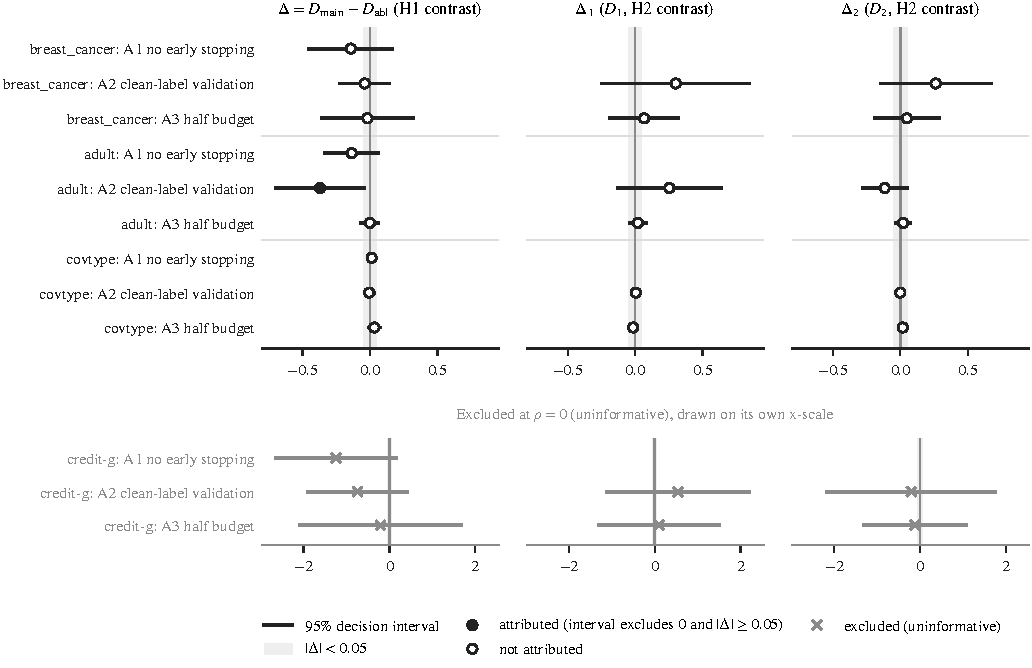
\includegraphics[width=\textwidth]{figures/fig_ablations.pdf}
\caption{Ablation tests. Each row is $\Delta = D_{\mathrm{main}} - D_{\mathrm{ablation}}$
for one ablation and dataset, with the dataset's 95\% paired $t(9)$ decision interval over
the same 10 seeds (variance corrected for re-splitting on \bc{} and \cg). The gray band marks
$|\Delta| < 0.05$. Markers give the pre-specified status: filled for attributed (the
interval excludes 0 and $|\Delta| \ge 0.05$), open for not attributed, and a cross for
excluded. One of the 21 tests on informative datasets is attributed: A2, H1 contrast, on
\ad. About one such interval is expected by chance at 95\% across 21 tests, and no
multiplicity correction was planned. A2 changes two things at once, the labels used for model
selection and the labels GBDT's early stopping monitors, so that result cannot be assigned to
model selection. A1 compares GBDT and GBDT without early stopping, which draw different
random candidate configurations. \cg{} (excluded) is drawn on its own x-scale. Its A1
headroom also failed the stability check.}
\label{fig:ablations}
\end{figure}

The ablations ask whether early stopping, noisy model selection or the size of the tuning
budget drives the contrasts (Table~\ref{tab:ablations}, Figure~\ref{fig:ablations}).

\paragraph{A1: no early stopping.} Not attributed on any informative dataset: \bc{}
$\Delta = \AOneDeltaBc$ [$\AOneDeltaBcLo$, $\AOneDeltaBcHi$], \ad{} $\AOneDeltaAd$
[$\AOneDeltaAdLo$, $\AOneDeltaAdHi$], and \ct{} $\AOneDeltaCt$ [$\AOneDeltaCtLo$,
$\AOneDeltaCtHi$]. On \ct{} the H1 contrast without early stopping is $D_{\mathrm{abl}} =
\AOneDablCt$ [$\AOneDablCtLo$, $\AOneDablCtHi$], close to the main $D$. The early-stopping and
no-early-stopping arms draw different random candidate configurations, so A1 mixes the
stopping rule with a different search. Without early stopping, the selected number of
iterations also falls with noise (median $\IterBcNeZero$ at $\rho=0$ and $\IterBcNeFour$ at
$\rho=0.4$ on \bc). The search itself chooses shorter boosting under noise.

\paragraph{A2: clean validation labels.} Under the pre-specified rule, the H1 contrast on
\ad{} is attributed: $\Delta = \ATwoDeltaAd$ [$\ATwoDeltaAdLo$, $\ATwoDeltaAdHi$]
($S = \ATwoDeltaAdS$, half-width $\ATwoDeltaAdHalf$). \textbf{This result cannot be assigned
to model selection.} A2 changes two things at once. It changes the labels used to choose
among candidates, and it changes the labels GBDT's early stopping monitors, so the GBDT
candidates under A2 are different fits. The ablation does not separate the two. It is
\textbf{one of the 21} ablation tests on informative datasets (A1 3, A2 9, A3 9)\footnote{The
counts in this sentence (21 tests, one attributed) are taken from the workspace's claim
\texttt{c-abl-count}, a text claim tied to the 21 status metrics. It has no generated macro,
so these counts are written in words.} and the only
one whose interval excludes 0. About one such interval is expected by chance at 95\% across
this many tests, and no multiplicity correction was planned. Its upper end, $\ATwoDeltaAdHi$,
lies on \ad's plain interval, which the design calls slightly narrow. The direction is that
the H1 gap is larger under clean-label selection and stopping ($D_{\mathrm{abl}} =
\ATwoDablAd$ [$\ATwoDablAdLo$, $\ATwoDablAdHi$]) than under the main procedure
($D = \HOneDAd$). RF's share of headroom lost falls from $\RAdRf$ to $\RAdRfCv$. The RF fits
are identical in the two procedures, so this part is a selection effect. GBDT's share rises
from $\RAdGb$ to $\RAdGbCv$, which mixes a change of fits with a change of selection. Every
other A2 test is not attributed. On \ct{} the clean-label H1 contrast is $D_{\mathrm{abl}} =
\ATwoDablCt$ [$\ATwoDablCtLo$, $\ATwoDablCtHi$], against $\Delta = \ATwoDeltaCt$
[$\ATwoDeltaCtLo$, $\ATwoDeltaCtHi$].

\paragraph{A3: half the budget.} Not attributed on any dataset. The largest point
estimates are on \bc: $\Delta_1 = \AThreeDeltaOneBc$ and $\Delta_2 = \AThreeDeltaTwoBc$. The interval
closest to excluding 0 is \ct's $\Delta_2 = \AThreeDeltaTwoCt$ [$\AThreeDeltaTwoCtLo$,
$\AThreeDeltaTwoCtHi$]. At this resolution, halving the budget changes no contrast by
enough to meet the rule. That includes the question of whether LR's one-dimensional search
gains more from 20 configurations than the trees' larger searches.

% ---------------------------------------------------------------------------
\section{Discussion and limitations}
\label{sec:discussion}

\paragraph{What the evidence supports.} On \ct, at 5,000-row subsamples with 3,000 training
rows, scikit-learn's log-loss GBDT with early stopping loses a larger share of its headroom
than a tuned random forest between $\rho=0$ and $\rho=0.4$. On \ct{} the forest is also the
more accurate method at every nonzero flip rate. That points the same way as the evidence
that boosting degrades more than forests or bagging \citep{dietterich2000,breiman2001,
nawaz2025}, but it is one dataset. The pre-specified count rule asks for more than that,
and the overall verdict is inconclusive. We make no claim that GBDT degrades more than RF in
general, or on \bc{} or \ad. Nor do we claim the reverse, as \citet{lebaher2020} found for
their untuned forests: no dataset contradicted H1. For H2, LR loses less than GBDT on \ct, but
it is not separable from RF there. LR also starts lower on \ct, and on \bc{} its point
estimate falls on the other side of RF's. The evidence does not support LR as the most
noise-robust of the three.

\paragraph{Resolution, not equivalence.} The inconclusive outcomes reflect the precision the
design can deliver. They do not show that the methods behave alike. No contrast on an
informative dataset reached ``no meaningful difference''. On \bc{} the re-splitting
correction gives a half-width of $\HOneDBcHalf$ for $D$, several times the 0.05 threshold.
This limit was stated before any run. A study that wants to decide H1 on small datasets
needs many more rows or a different design, not more seeds alone. On re-split data the
correction factor keeps the half-width from shrinking below about $1.13\,S$ however many
seeds are run.

\paragraph{Limitations.}
\begin{itemize}
  \item \textbf{Scope.} Four datasets, at most 3,000 training rows, scikit-learn~1.9.1,
  symmetric noise and accuracy. The GBDT arm is \texttt{HistGradientBoostingClassifier} on
  one-hot categoricals, with early stopping that keeps the 20 post-plateau iterations. The
  results say nothing about full-size \ad{} or \ct, about XGBoost, LightGBM or CatBoost or
  other stopping rules, about class-dependent noise, or about other metrics.
  \item \textbf{Three informative datasets.} With \cg{} excluded, H1 needed support on every
  remaining dataset. The design anticipated this, and it makes an inconclusive overall
  verdict likely whenever one dataset is underpowered.
  \item \textbf{Interval approximations.} The correction on \bc{} and \cg{} assumes a fixed
  correlation between re-splits. The plain interval on \ad{} ignores the training-row
  overlap between seeds (about 6\% by design arithmetic) and is slightly narrow. The single attributed ablation lies on that
  interval.
  \item \textbf{Ablation design.} A2 does not separate model selection from GBDT's
  early-stopping monitor. A1 compares different random candidate lists. Neither can isolate
  a mechanism. Across the 21 ablation tests no multiplicity correction was planned or
  applied.
  \item \textbf{Equal budget is not equal tuning.} LR searches one dimension and the trees
  three or four, and GBDT's early stopping adds a free choice of the number of iterations.
  A1 and A3 probe this but did not resolve it.
  \item \textbf{Rare classes.} On \ct{} the smallest class has about 5 test rows per seed (by
  design arithmetic),
  and accuracy is dominated by the two largest classes.
  \item \textbf{Replication: passed, on the same machine.} After the results were final, a
  clean rerun re-executed every logged run (20 runs, a count of the replication ledger) in a
  fresh environment built from \texttt{code/requirements.txt} alone, with all three
  downloaded datasets fetched again from OpenML and figshare. Every recorded metric
  reproduced to a relative tolerance of $10^{-6}$ (absolute $10^{-9}$), with no mismatch
  and no failed run (\texttt{replication.json}, 2026-11-18; \texttt{REPLICATION.md}). The
  rerun used the same laptop and operating system as the original runs, so it shows that
  the results follow from the logged code, pinned packages and pinned data; it does not
  show that they are bit-identical on other hardware, operating systems or BLAS builds.
  Fit times are not metrics and were not compared.
\end{itemize}

% ---------------------------------------------------------------------------
\section{Deviations from the approved design and disclosures}
\label{sec:deviations}

During execution we made no deviation from the design approved at the design gate. The
compute contingency was evaluated as written and did not trigger. The fixes from the code
review were exact threshold comparisons and input/output hashing. They were made before the
first analysis run and change no rule. The following departures and decisions are recorded
in \texttt{plan.json}. Items 1 and 2 include a correction that the PI appended at the paper
stage, after the paper review found the original entries wrong; the original entries are
left unedited in \texttt{plan.json}. We list all of them.
\begin{enumerate}
  \item \textbf{The Reviewer's pre-gate pilot, which included a study dataset.} During the
  first review of the research question, before the hypotheses were fixed, the Reviewer
  agent ran a pilot of the three methods outside the workspace: untuned scikit-learn
  defaults, 5 seeds, an 80/20 split and 40\% flips. It used four datasets: iris, wine,
  digits and \bc. \bc{} is a study dataset. On it, GBDT lost about 5 accuracy points more
  than RF at 40\% noise, the direction H1 later predicted. The pilot's results informed the
  revised question (per-dataset reporting and decision rules). Our earlier records stated
  that no study dataset was piloted. That was wrong: the PI relied on the Reviewer's summary
  rather than its review file. Readers should weigh \bc{} with this in mind; its H1
  outcome under the pre-specified interval is no detectable difference (inconclusive).
  \item \textbf{Datasets that depart from the brief.} The seed brief asked for datasets that
  ship with scikit-learn. Its bundled classification sets are iris, wine, digits and \bc.
  \bc{} stayed in the study because the brief requires a dataset bundled with scikit-learn.
  Iris, wine and digits were left out; the original record gives their use in the pilot as
  the reason, and digits is image data. Because \bc{} was piloted too (item~1), the
  selection was not pilot-blind. The PI added three
  tabular datasets retrieved through scikit-learn loaders: \ad{} and \ct, because prior
  label-noise studies used them \citep{lebaher2020,eisenburger2024}, and \cg, a small
  imbalanced dataset with no prior label-noise study that we found. The exact versions and
  hashes were pinned before any analysis run.
  \item \textbf{Validation labels flipped.} The brief says that noise is injected into
  training labels only and that test labels stay clean. Test labels stay clean, but the
  validation labels used for tuning and early stopping are flipped at the training rate,
  because a practitioner's labelled data are noisy throughout. Ablation A2 gives the
  clean-validation variant at $\rho=0.4$.
  \item \textbf{What ``no difference'' means.} The brief asks that differences inside the
  noise be reported as no difference. A difference whose interval includes 0 is never
  reported as a difference. We write ``no meaningful difference'' only when the whole
  interval lies inside $(-0.05, 0.05)$. Otherwise we write ``no detectable difference
  (inconclusive)'', because a wide interval does not show that the methods behave alike.
  \item \textbf{Hardware.} We read ``laptop CPU'' as the PI's laptop: an Apple M3 with
  8 cores (4 performance and 4 efficiency), run with 8 worker processes. The design
  estimate of about 134 CPU-minutes implies that a machine with fewer than about 3 cores
  would not fit the one-hour budget. That bound comes from the estimate, not from measured
  times; the measured CPU time is in \texttt{runs/NOTES.md}.
  \item \textbf{Interval change.} The approved hypotheses named a 95\% percentile interval
  from a paired bootstrap over seeds. Following two design reviews, and before any analysis
  run, the design replaced it with the paired $t(9)$ interval of
  Section~\ref{sec:setup}. That interval is variance corrected on \bc{} and \cg{} and plain
  on \ad{} and \ct. The bootstrap, which under-covers with 10 seeds, is kept only as a
  descriptive check. Thresholds, exclusion and count rules are unchanged. The design records
  call this correction ``Nadeau--Bengio''. Section~\ref{sec:setup} explains why we do not
  attribute the formula to \citet{nadeau2003}.
\end{enumerate}

% ---------------------------------------------------------------------------
\section{Conclusion}
\label{sec:conclusion}

Under exact symmetric label noise, an equal tuning budget on noisy validation labels and
clean test labels, we could not decide either pre-specified hypothesis. Log-loss gradient
boosting with early stopping lost a larger share of its headroom than a random forest on
\ct{} alone. The other two informative datasets gave no detectable difference, and the
fourth was excluded before any noisy run. Logistic regression was not shown to be the most
robust of the three on any dataset. The ablations attribute no mechanism we can interpret.
The study's value is the protocol and its fully logged runs, which a clean rerun
reproduced metric for metric. It also gives a concrete
measure of how wide the intervals are at these sample sizes, which a future study of the
same question should plan for.

\section*{AI-use statement}

This paper was drafted by a crew of AI research-assistant agents
(Free-Research-Crew, protocol v0.1) under the direction of the human author, Bryce Wang.
He approved the research question, the design and the results at three human gates, and
the manuscript itself is subject to a fourth, the submission gate. He takes responsibility
for the paper's content.

\begin{itemize}
  \item \textbf{Roles and models.} Every crew role ran on Anthropic Claude through Claude
        Code. The PI role was the main Claude Code session. The Scout, Designer, Data RA,
        Experimenter, Figures RA, Reviewer, Writer and Replicator ran as subagents launched
        from that session. The review records name the model as \texttt{claude-opus-5-5}.
        The Replicator reran every logged run (20 runs, a count of the replication ledger)
        in a fresh environment from the pinned requirements, with the data downloaded again,
        on the same laptop. Every recorded metric reproduced to a relative tolerance of
        $10^{-6}$ (\texttt{replication.json}, 2026-11-18).
  \item \textbf{Review.} The Reviewer agent ran 4 rounds on the research question, 3 on the
        design, 1 on the code, 2 on the results and, so far, 1 on the paper. This version
        answers that paper review, which comes before the submission gate. Its independence level was \emph{fresh-context}: a new context in
        every round, with the same model family as the other roles. The human author chose
        this over a cross-family reviewer. In the last question round the Reviewer still
        recommended revision, with two findings open. The human approved the question gate
        with those findings open, and the design then addressed both; the first design
        review recorded them as handled. In two cases the authors narrowed a claim instead
        of changing the analysis, and the Reviewer recorded the finding as conceded: a
        dropped ranking-reversal hypothesis at the question stage, and the A2 wording at
        the results stage.
  \item \textbf{Findings accepted over the Reviewer's objection.} None.
  \item \textbf{Evidence.} Every reported number is a macro generated from the metrics of
        a logged run, and none was typed by hand. Every citation was checked against its
        source. Where only the abstract could be read, the paper says no more than the
        abstract does. The full workspace is public at
        \url{https://github.com/brycewang-stanford/Free-Research-Crew/tree/main/gallery/cs-label-noise}.
        It contains the plan, the run ledger, the code, the data manifest, every review and
        this paper's sources.
\end{itemize}


\bibliographystyle{plainnat}
\bibliography{../refs}

% ---------------------------------------------------------------------------
\appendix
\section{Additional tables}

\begin{table}[!htbp]
\centering
\resizebox{\textwidth}{!}{% Generated by code/tab_accuracy.py from logged runs. Do not edit by hand; rerun the script.
% Needs \usepackage{booktabs,array} and % Generated by `crew.py numbers` from claims.jsonl. Do not edit by hand.
% Each macro is a number taken from a logged run; see claims.jsonl.
\newcommand{\NCells}{600}  % c-n-cells
\newcommand{\NFlipFail}{0}  % c-flip-fail
\newcommand{\NConvWarnCells}{0}  % c-convwarn
\newcommand{\MajBc}{0.632}  % c-m-Bc
\newcommand{\AccBcLrZero}{0.970}  % c-acc-Bc-Lr-Zero
\newcommand{\SdBcLrZero}{0.010}  % c-sd-Bc-Lr-Zero
\newcommand{\PmsBcLrZero}{0.651}  % c-pms-Bc-Lr-Zero
\newcommand{\VnBcLrZero}{0.975}  % c-vn-Bc-Lr-Zero
\newcommand{\VcBcLrZero}{0.975}  % c-vc-Bc-Lr-Zero
\newcommand{\TnBcLrZero}{0.987}  % c-tn-Bc-Lr-Zero
\newcommand{\CBcZero}{0.276}  % c-C-Bc-Zero
\newcommand{\AccBcLrOne}{0.954}  % c-acc-Bc-Lr-One
\newcommand{\SdBcLrOne}{0.029}  % c-sd-Bc-Lr-One
\newcommand{\PmsBcLrOne}{0.665}  % c-pms-Bc-Lr-One
\newcommand{\VnBcLrOne}{0.875}  % c-vn-Bc-Lr-One
\newcommand{\VcBcLrOne}{0.954}  % c-vc-Bc-Lr-One
\newcommand{\TnBcLrOne}{0.875}  % c-tn-Bc-Lr-One
\newcommand{\CBcOne}{0.104}  % c-C-Bc-One
\newcommand{\AccBcLrTwo}{0.949}  % c-acc-Bc-Lr-Two
\newcommand{\SdBcLrTwo}{0.020}  % c-sd-Bc-Lr-Two
\newcommand{\PmsBcLrTwo}{0.667}  % c-pms-Bc-Lr-Two
\newcommand{\VnBcLrTwo}{0.777}  % c-vn-Bc-Lr-Two
\newcommand{\VcBcLrTwo}{0.953}  % c-vc-Bc-Lr-Two
\newcommand{\TnBcLrTwo}{0.777}  % c-tn-Bc-Lr-Two
\newcommand{\CBcTwo}{0.0492}  % c-C-Bc-Two
\newcommand{\AccBcLrThree}{0.907}  % c-acc-Bc-Lr-Three
\newcommand{\SdBcLrThree}{0.027}  % c-sd-Bc-Lr-Three
\newcommand{\PmsBcLrThree}{0.672}  % c-pms-Bc-Lr-Three
\newcommand{\VnBcLrThree}{0.689}  % c-vn-Bc-Lr-Three
\newcommand{\VcBcLrThree}{0.909}  % c-vc-Bc-Lr-Three
\newcommand{\TnBcLrThree}{0.684}  % c-tn-Bc-Lr-Three
\newcommand{\CBcThree}{0.051}  % c-C-Bc-Three
\newcommand{\AccBcLrFour}{0.781}  % c-acc-Bc-Lr-Four
\newcommand{\SdBcLrFour}{0.098}  % c-sd-Bc-Lr-Four
\newcommand{\PmsBcLrFour}{0.670}  % c-pms-Bc-Lr-Four
\newcommand{\VnBcLrFour}{0.597}  % c-vn-Bc-Lr-Four
\newcommand{\VcBcLrFour}{0.764}  % c-vc-Bc-Lr-Four
\newcommand{\TnBcLrFour}{0.593}  % c-tn-Bc-Lr-Four
\newcommand{\CBcFour}{0.0428}  % c-C-Bc-Four
\newcommand{\AccBcRfZero}{0.951}  % c-acc-Bc-Rf-Zero
\newcommand{\SdBcRfZero}{0.032}  % c-sd-Bc-Rf-Zero
\newcommand{\PmsBcRfZero}{0.633}  % c-pms-Bc-Rf-Zero
\newcommand{\VnBcRfZero}{0.961}  % c-vn-Bc-Rf-Zero
\newcommand{\VcBcRfZero}{0.961}  % c-vc-Bc-Rf-Zero
\newcommand{\TnBcRfZero}{0.988}  % c-tn-Bc-Rf-Zero
\newcommand{\MslBcZero}{2.5}  % c-msl-Bc-Zero
\newcommand{\MfBcZero}{0.24}  % c-mf-Bc-Zero
\newcommand{\AccBcRfOne}{0.948}  % c-acc-Bc-Rf-One
\newcommand{\SdBcRfOne}{0.027}  % c-sd-Bc-Rf-One
\newcommand{\PmsBcRfOne}{0.632}  % c-pms-Bc-Rf-One
\newcommand{\VnBcRfOne}{0.877}  % c-vn-Bc-Rf-One
\newcommand{\VcBcRfOne}{0.958}  % c-vc-Bc-Rf-One
\newcommand{\TnBcRfOne}{0.921}  % c-tn-Bc-Rf-One
\newcommand{\MslBcOne}{3}  % c-msl-Bc-One
\newcommand{\MfBcOne}{0.40}  % c-mf-Bc-One
\newcommand{\AccBcRfTwo}{0.943}  % c-acc-Bc-Rf-Two
\newcommand{\SdBcRfTwo}{0.033}  % c-sd-Bc-Rf-Two
\newcommand{\PmsBcRfTwo}{0.627}  % c-pms-Bc-Rf-Two
\newcommand{\VnBcRfTwo}{0.792}  % c-vn-Bc-Rf-Two
\newcommand{\VcBcRfTwo}{0.954}  % c-vc-Bc-Rf-Two
\newcommand{\TnBcRfTwo}{0.876}  % c-tn-Bc-Rf-Two
\newcommand{\MslBcTwo}{6.5}  % c-msl-Bc-Two
\newcommand{\MfBcTwo}{0.20}  % c-mf-Bc-Two
\newcommand{\AccBcRfThree}{0.922}  % c-acc-Bc-Rf-Three
\newcommand{\SdBcRfThree}{0.026}  % c-sd-Bc-Rf-Three
\newcommand{\PmsBcRfThree}{0.636}  % c-pms-Bc-Rf-Three
\newcommand{\VnBcRfThree}{0.704}  % c-vn-Bc-Rf-Three
\newcommand{\VcBcRfThree}{0.923}  % c-vc-Bc-Rf-Three
\newcommand{\TnBcRfThree}{0.764}  % c-tn-Bc-Rf-Three
\newcommand{\MslBcThree}{15}  % c-msl-Bc-Three
\newcommand{\MfBcThree}{0.49}  % c-mf-Bc-Three
\newcommand{\AccBcRfFour}{0.846}  % c-acc-Bc-Rf-Four
\newcommand{\SdBcRfFour}{0.074}  % c-sd-Bc-Rf-Four
\newcommand{\PmsBcRfFour}{0.581}  % c-pms-Bc-Rf-Four
\newcommand{\VnBcRfFour}{0.596}  % c-vn-Bc-Rf-Four
\newcommand{\VcBcRfFour}{0.834}  % c-vc-Bc-Rf-Four
\newcommand{\TnBcRfFour}{0.755}  % c-tn-Bc-Rf-Four
\newcommand{\MslBcFour}{19.5}  % c-msl-Bc-Four
\newcommand{\MfBcFour}{0.38}  % c-mf-Bc-Four
\newcommand{\AccBcGbZero}{0.954}  % c-acc-Bc-Gb-Zero
\newcommand{\SdBcGbZero}{0.031}  % c-sd-Bc-Gb-Zero
\newcommand{\PmsBcGbZero}{0.632}  % c-pms-Bc-Gb-Zero
\newcommand{\VnBcGbZero}{0.975}  % c-vn-Bc-Gb-Zero
\newcommand{\VcBcGbZero}{0.975}  % c-vc-Bc-Gb-Zero
\newcommand{\TnBcGbZero}{1.000}  % c-tn-Bc-Gb-Zero
\newcommand{\LrateBcZero}{0.057}  % c-lrate-Bc-Zero
\newcommand{\IterBcZero}{167}  % c-iter-Bc-Zero
\newcommand{\AccBcGbOne}{0.942}  % c-acc-Bc-Gb-One
\newcommand{\SdBcGbOne}{0.033}  % c-sd-Bc-Gb-One
\newcommand{\PmsBcGbOne}{0.625}  % c-pms-Bc-Gb-One
\newcommand{\VnBcGbOne}{0.882}  % c-vn-Bc-Gb-One
\newcommand{\VcBcGbOne}{0.958}  % c-vc-Bc-Gb-One
\newcommand{\TnBcGbOne}{0.964}  % c-tn-Bc-Gb-One
\newcommand{\LrateBcOne}{0.0728}  % c-lrate-Bc-One
\newcommand{\IterBcOne}{62}  % c-iter-Bc-One
\newcommand{\AccBcGbTwo}{0.927}  % c-acc-Bc-Gb-Two
\newcommand{\SdBcGbTwo}{0.044}  % c-sd-Bc-Gb-Two
\newcommand{\PmsBcGbTwo}{0.625}  % c-pms-Bc-Gb-Two
\newcommand{\VnBcGbTwo}{0.782}  % c-vn-Bc-Gb-Two
\newcommand{\VcBcGbTwo}{0.939}  % c-vc-Bc-Gb-Two
\newcommand{\TnBcGbTwo}{0.889}  % c-tn-Bc-Gb-Two
\newcommand{\LrateBcTwo}{0.0743}  % c-lrate-Bc-Two
\newcommand{\IterBcTwo}{54}  % c-iter-Bc-Two
\newcommand{\AccBcGbThree}{0.911}  % c-acc-Bc-Gb-Three
\newcommand{\SdBcGbThree}{0.045}  % c-sd-Bc-Gb-Three
\newcommand{\PmsBcGbThree}{0.629}  % c-pms-Bc-Gb-Three
\newcommand{\VnBcGbThree}{0.698}  % c-vn-Bc-Gb-Three
\newcommand{\VcBcGbThree}{0.918}  % c-vc-Bc-Gb-Three
\newcommand{\TnBcGbThree}{0.752}  % c-tn-Bc-Gb-Three
\newcommand{\LrateBcThree}{0.0233}  % c-lrate-Bc-Three
\newcommand{\IterBcThree}{82}  % c-iter-Bc-Three
\newcommand{\AccBcGbFour}{0.762}  % c-acc-Bc-Gb-Four
\newcommand{\SdBcGbFour}{0.079}  % c-sd-Bc-Gb-Four
\newcommand{\PmsBcGbFour}{0.568}  % c-pms-Bc-Gb-Four
\newcommand{\VnBcGbFour}{0.604}  % c-vn-Bc-Gb-Four
\newcommand{\VcBcGbFour}{0.756}  % c-vc-Bc-Gb-Four
\newcommand{\TnBcGbFour}{0.800}  % c-tn-Bc-Gb-Four
\newcommand{\LrateBcFour}{0.0717}  % c-lrate-Bc-Four
\newcommand{\IterBcFour}{31}  % c-iter-Bc-Four
\newcommand{\MajCg}{0.700}  % c-m-Cg
\newcommand{\AccCgLrZero}{0.750}  % c-acc-Cg-Lr-Zero
\newcommand{\SdCgLrZero}{0.018}  % c-sd-Cg-Lr-Zero
\newcommand{\PmsCgLrZero}{0.795}  % c-pms-Cg-Lr-Zero
\newcommand{\VnCgLrZero}{0.762}  % c-vn-Cg-Lr-Zero
\newcommand{\VcCgLrZero}{0.762}  % c-vc-Cg-Lr-Zero
\newcommand{\TnCgLrZero}{0.788}  % c-tn-Cg-Lr-Zero
\newcommand{\CCgZero}{0.272}  % c-C-Cg-Zero
\newcommand{\AccCgLrOne}{0.741}  % c-acc-Cg-Lr-One
\newcommand{\SdCgLrOne}{0.016}  % c-sd-Cg-Lr-One
\newcommand{\PmsCgLrOne}{0.793}  % c-pms-Cg-Lr-One
\newcommand{\VnCgLrOne}{0.718}  % c-vn-Cg-Lr-One
\newcommand{\VcCgLrOne}{0.758}  % c-vc-Cg-Lr-One
\newcommand{\TnCgLrOne}{0.739}  % c-tn-Cg-Lr-One
\newcommand{\CCgOne}{0.255}  % c-C-Cg-One
\newcommand{\AccCgLrTwo}{0.715}  % c-acc-Cg-Lr-Two
\newcommand{\SdCgLrTwo}{0.019}  % c-sd-Cg-Lr-Two
\newcommand{\PmsCgLrTwo}{0.839}  % c-pms-Cg-Lr-Two
\newcommand{\VnCgLrTwo}{0.666}  % c-vn-Cg-Lr-Two
\newcommand{\VcCgLrTwo}{0.734}  % c-vc-Cg-Lr-Two
\newcommand{\TnCgLrTwo}{0.677}  % c-tn-Cg-Lr-Two
\newcommand{\CCgTwo}{0.0654}  % c-C-Cg-Two
\newcommand{\AccCgLrThree}{0.710}  % c-acc-Cg-Lr-Three
\newcommand{\SdCgLrThree}{0.028}  % c-sd-Cg-Lr-Three
\newcommand{\PmsCgLrThree}{0.839}  % c-pms-Cg-Lr-Three
\newcommand{\VnCgLrThree}{0.611}  % c-vn-Cg-Lr-Three
\newcommand{\VcCgLrThree}{0.718}  % c-vc-Cg-Lr-Three
\newcommand{\TnCgLrThree}{0.635}  % c-tn-Cg-Lr-Three
\newcommand{\CCgThree}{0.0336}  % c-C-Cg-Three
\newcommand{\AccCgLrFour}{0.674}  % c-acc-Cg-Lr-Four
\newcommand{\SdCgLrFour}{0.053}  % c-sd-Cg-Lr-Four
\newcommand{\PmsCgLrFour}{0.867}  % c-pms-Cg-Lr-Four
\newcommand{\VnCgLrFour}{0.576}  % c-vn-Cg-Lr-Four
\newcommand{\VcCgLrFour}{0.683}  % c-vc-Cg-Lr-Four
\newcommand{\TnCgLrFour}{0.572}  % c-tn-Cg-Lr-Four
\newcommand{\CCgFour}{0.00698}  % c-C-Cg-Four
\newcommand{\AccCgRfZero}{0.749}  % c-acc-Cg-Rf-Zero
\newcommand{\SdCgRfZero}{0.020}  % c-sd-Cg-Rf-Zero
\newcommand{\PmsCgRfZero}{0.823}  % c-pms-Cg-Rf-Zero
\newcommand{\VnCgRfZero}{0.781}  % c-vn-Cg-Rf-Zero
\newcommand{\VcCgRfZero}{0.781}  % c-vc-Cg-Rf-Zero
\newcommand{\TnCgRfZero}{0.929}  % c-tn-Cg-Rf-Zero
\newcommand{\MslCgZero}{2}  % c-msl-Cg-Zero
\newcommand{\MfCgZero}{0.26}  % c-mf-Cg-Zero
\newcommand{\AccCgRfOne}{0.739}  % c-acc-Cg-Rf-One
\newcommand{\SdCgRfOne}{0.019}  % c-sd-Cg-Rf-One
\newcommand{\PmsCgRfOne}{0.828}  % c-pms-Cg-Rf-One
\newcommand{\VnCgRfOne}{0.725}  % c-vn-Cg-Rf-One
\newcommand{\VcCgRfOne}{0.767}  % c-vc-Cg-Rf-One
\newcommand{\TnCgRfOne}{0.882}  % c-tn-Cg-Rf-One
\newcommand{\MslCgOne}{5.5}  % c-msl-Cg-One
\newcommand{\MfCgOne}{0.29}  % c-mf-Cg-One
\newcommand{\AccCgRfTwo}{0.731}  % c-acc-Cg-Rf-Two
\newcommand{\SdCgRfTwo}{0.017}  % c-sd-Cg-Rf-Two
\newcommand{\PmsCgRfTwo}{0.815}  % c-pms-Cg-Rf-Two
\newcommand{\VnCgRfTwo}{0.681}  % c-vn-Cg-Rf-Two
\newcommand{\VcCgRfTwo}{0.753}  % c-vc-Cg-Rf-Two
\newcommand{\TnCgRfTwo}{0.853}  % c-tn-Cg-Rf-Two
\newcommand{\MslCgTwo}{4.5}  % c-msl-Cg-Two
\newcommand{\MfCgTwo}{0.28}  % c-mf-Cg-Two
\newcommand{\AccCgRfThree}{0.703}  % c-acc-Cg-Rf-Three
\newcommand{\SdCgRfThree}{0.031}  % c-sd-Cg-Rf-Three
\newcommand{\PmsCgRfThree}{0.843}  % c-pms-Cg-Rf-Three
\newcommand{\VnCgRfThree}{0.629}  % c-vn-Cg-Rf-Three
\newcommand{\VcCgRfThree}{0.725}  % c-vc-Cg-Rf-Three
\newcommand{\TnCgRfThree}{0.773}  % c-tn-Cg-Rf-Three
\newcommand{\MslCgThree}{9}  % c-msl-Cg-Three
\newcommand{\MfCgThree}{0.30}  % c-mf-Cg-Three
\newcommand{\AccCgRfFour}{0.638}  % c-acc-Cg-Rf-Four
\newcommand{\SdCgRfFour}{0.047}  % c-sd-Cg-Rf-Four
\newcommand{\PmsCgRfFour}{0.728}  % c-pms-Cg-Rf-Four
\newcommand{\VnCgRfFour}{0.585}  % c-vn-Cg-Rf-Four
\newcommand{\VcCgRfFour}{0.661}  % c-vc-Cg-Rf-Four
\newcommand{\TnCgRfFour}{0.732}  % c-tn-Cg-Rf-Four
\newcommand{\MslCgFour}{15.5}  % c-msl-Cg-Four
\newcommand{\MfCgFour}{0.32}  % c-mf-Cg-Four
\newcommand{\AccCgGbZero}{0.735}  % c-acc-Cg-Gb-Zero
\newcommand{\SdCgGbZero}{0.016}  % c-sd-Cg-Gb-Zero
\newcommand{\PmsCgGbZero}{0.791}  % c-pms-Cg-Gb-Zero
\newcommand{\VnCgGbZero}{0.783}  % c-vn-Cg-Gb-Zero
\newcommand{\VcCgGbZero}{0.783}  % c-vc-Cg-Gb-Zero
\newcommand{\TnCgGbZero}{0.932}  % c-tn-Cg-Gb-Zero
\newcommand{\LrateCgZero}{0.158}  % c-lrate-Cg-Zero
\newcommand{\IterCgZero}{56}  % c-iter-Cg-Zero
\newcommand{\AccCgGbOne}{0.729}  % c-acc-Cg-Gb-One
\newcommand{\SdCgGbOne}{0.026}  % c-sd-Cg-Gb-One
\newcommand{\PmsCgGbOne}{0.779}  % c-pms-Cg-Gb-One
\newcommand{\VnCgGbOne}{0.730}  % c-vn-Cg-Gb-One
\newcommand{\VcCgGbOne}{0.764}  % c-vc-Cg-Gb-One
\newcommand{\TnCgGbOne}{0.856}  % c-tn-Cg-Gb-One
\newcommand{\LrateCgOne}{0.044}  % c-lrate-Cg-One
\newcommand{\IterCgOne}{76}  % c-iter-Cg-One
\newcommand{\AccCgGbTwo}{0.714}  % c-acc-Cg-Gb-Two
\newcommand{\SdCgGbTwo}{0.018}  % c-sd-Cg-Gb-Two
\newcommand{\PmsCgGbTwo}{0.797}  % c-pms-Cg-Gb-Two
\newcommand{\VnCgGbTwo}{0.684}  % c-vn-Cg-Gb-Two
\newcommand{\VcCgGbTwo}{0.742}  % c-vc-Cg-Gb-Two
\newcommand{\TnCgGbTwo}{0.793}  % c-tn-Cg-Gb-Two
\newcommand{\LrateCgTwo}{0.0254}  % c-lrate-Cg-Two
\newcommand{\IterCgTwo}{102}  % c-iter-Cg-Two
\newcommand{\AccCgGbThree}{0.692}  % c-acc-Cg-Gb-Three
\newcommand{\SdCgGbThree}{0.027}  % c-sd-Cg-Gb-Three
\newcommand{\PmsCgGbThree}{0.793}  % c-pms-Cg-Gb-Three
\newcommand{\VnCgGbThree}{0.626}  % c-vn-Cg-Gb-Three
\newcommand{\VcCgGbThree}{0.705}  % c-vc-Cg-Gb-Three
\newcommand{\TnCgGbThree}{0.728}  % c-tn-Cg-Gb-Three
\newcommand{\LrateCgThree}{0.0316}  % c-lrate-Cg-Three
\newcommand{\IterCgThree}{53}  % c-iter-Cg-Three
\newcommand{\AccCgGbFour}{0.647}  % c-acc-Cg-Gb-Four
\newcommand{\SdCgGbFour}{0.046}  % c-sd-Cg-Gb-Four
\newcommand{\PmsCgGbFour}{0.783}  % c-pms-Cg-Gb-Four
\newcommand{\VnCgGbFour}{0.581}  % c-vn-Cg-Gb-Four
\newcommand{\VcCgGbFour}{0.651}  % c-vc-Cg-Gb-Four
\newcommand{\TnCgGbFour}{0.667}  % c-tn-Cg-Gb-Four
\newcommand{\LrateCgFour}{0.0251}  % c-lrate-Cg-Four
\newcommand{\IterCgFour}{29}  % c-iter-Cg-Four
\newcommand{\MajAd}{0.761}  % c-m-Ad
\newcommand{\AccAdLrZero}{0.843}  % c-acc-Ad-Lr-Zero
\newcommand{\SdAdLrZero}{0.012}  % c-sd-Ad-Lr-Zero
\newcommand{\PmsAdLrZero}{0.812}  % c-pms-Ad-Lr-Zero
\newcommand{\VnAdLrZero}{0.849}  % c-vn-Ad-Lr-Zero
\newcommand{\VcAdLrZero}{0.849}  % c-vc-Ad-Lr-Zero
\newcommand{\TnAdLrZero}{0.855}  % c-tn-Ad-Lr-Zero
\newcommand{\CAdZero}{0.38}  % c-C-Ad-Zero
\newcommand{\AccAdLrOne}{0.838}  % c-acc-Ad-Lr-One
\newcommand{\SdAdLrOne}{0.010}  % c-sd-Ad-Lr-One
\newcommand{\PmsAdLrOne}{0.822}  % c-pms-Ad-Lr-One
\newcommand{\VnAdLrOne}{0.776}  % c-vn-Ad-Lr-One
\newcommand{\VcAdLrOne}{0.844}  % c-vc-Ad-Lr-One
\newcommand{\TnAdLrOne}{0.780}  % c-tn-Ad-Lr-One
\newcommand{\CAdOne}{0.182}  % c-C-Ad-One
\newcommand{\AccAdLrTwo}{0.830}  % c-acc-Ad-Lr-Two
\newcommand{\SdAdLrTwo}{0.009}  % c-sd-Ad-Lr-Two
\newcommand{\PmsAdLrTwo}{0.848}  % c-pms-Ad-Lr-Two
\newcommand{\VnAdLrTwo}{0.703}  % c-vn-Ad-Lr-Two
\newcommand{\VcAdLrTwo}{0.833}  % c-vc-Ad-Lr-Two
\newcommand{\TnAdLrTwo}{0.703}  % c-tn-Ad-Lr-Two
\newcommand{\CAdTwo}{0.0195}  % c-C-Ad-Two
\newcommand{\AccAdLrThree}{0.821}  % c-acc-Ad-Lr-Three
\newcommand{\SdAdLrThree}{0.009}  % c-sd-Ad-Lr-Three
\newcommand{\PmsAdLrThree}{0.847}  % c-pms-Ad-Lr-Three
\newcommand{\VnAdLrThree}{0.637}  % c-vn-Ad-Lr-Three
\newcommand{\VcAdLrThree}{0.823}  % c-vc-Ad-Lr-Three
\newcommand{\TnAdLrThree}{0.637}  % c-tn-Ad-Lr-Three
\newcommand{\CAdThree}{0.0202}  % c-C-Ad-Three
\newcommand{\AccAdLrFour}{0.797}  % c-acc-Ad-Lr-Four
\newcommand{\SdAdLrFour}{0.015}  % c-sd-Ad-Lr-Four
\newcommand{\PmsAdLrFour}{0.833}  % c-pms-Ad-Lr-Four
\newcommand{\VnAdLrFour}{0.569}  % c-vn-Ad-Lr-Four
\newcommand{\VcAdLrFour}{0.804}  % c-vc-Ad-Lr-Four
\newcommand{\TnAdLrFour}{0.572}  % c-tn-Ad-Lr-Four
\newcommand{\CAdFour}{0.00584}  % c-C-Ad-Four
\newcommand{\AccAdRfZero}{0.847}  % c-acc-Ad-Rf-Zero
\newcommand{\SdAdRfZero}{0.010}  % c-sd-Ad-Rf-Zero
\newcommand{\PmsAdRfZero}{0.814}  % c-pms-Ad-Rf-Zero
\newcommand{\VnAdRfZero}{0.859}  % c-vn-Ad-Rf-Zero
\newcommand{\VcAdRfZero}{0.859}  % c-vc-Ad-Rf-Zero
\newcommand{\TnAdRfZero}{0.911}  % c-tn-Ad-Rf-Zero
\newcommand{\MslAdZero}{3}  % c-msl-Ad-Zero
\newcommand{\MfAdZero}{0.20}  % c-mf-Ad-Zero
\newcommand{\AccAdRfOne}{0.845}  % c-acc-Ad-Rf-One
\newcommand{\SdAdRfOne}{0.012}  % c-sd-Ad-Rf-One
\newcommand{\PmsAdRfOne}{0.812}  % c-pms-Ad-Rf-One
\newcommand{\VnAdRfOne}{0.788}  % c-vn-Ad-Rf-One
\newcommand{\VcAdRfOne}{0.855}  % c-vc-Ad-Rf-One
\newcommand{\TnAdRfOne}{0.829}  % c-tn-Ad-Rf-One
\newcommand{\MslAdOne}{3.5}  % c-msl-Ad-One
\newcommand{\MfAdOne}{0.22}  % c-mf-Ad-One
\newcommand{\AccAdRfTwo}{0.836}  % c-acc-Ad-Rf-Two
\newcommand{\SdAdRfTwo}{0.006}  % c-sd-Ad-Rf-Two
\newcommand{\PmsAdRfTwo}{0.823}  % c-pms-Ad-Rf-Two
\newcommand{\VnAdRfTwo}{0.714}  % c-vn-Ad-Rf-Two
\newcommand{\VcAdRfTwo}{0.847}  % c-vc-Ad-Rf-Two
\newcommand{\TnAdRfTwo}{0.760}  % c-tn-Ad-Rf-Two
\newcommand{\MslAdTwo}{2.5}  % c-msl-Ad-Two
\newcommand{\MfAdTwo}{0.11}  % c-mf-Ad-Two
\newcommand{\AccAdRfThree}{0.830}  % c-acc-Ad-Rf-Three
\newcommand{\SdAdRfThree}{0.016}  % c-sd-Ad-Rf-Three
\newcommand{\PmsAdRfThree}{0.809}  % c-pms-Ad-Rf-Three
\newcommand{\VnAdRfThree}{0.644}  % c-vn-Ad-Rf-Three
\newcommand{\VcAdRfThree}{0.834}  % c-vc-Ad-Rf-Three
\newcommand{\TnAdRfThree}{0.715}  % c-tn-Ad-Rf-Three
\newcommand{\MslAdThree}{11}  % c-msl-Ad-Three
\newcommand{\MfAdThree}{0.13}  % c-mf-Ad-Three
\newcommand{\AccAdRfFour}{0.794}  % c-acc-Ad-Rf-Four
\newcommand{\SdAdRfFour}{0.021}  % c-sd-Ad-Rf-Four
\newcommand{\PmsAdRfFour}{0.776}  % c-pms-Ad-Rf-Four
\newcommand{\VnAdRfFour}{0.571}  % c-vn-Ad-Rf-Four
\newcommand{\VcAdRfFour}{0.804}  % c-vc-Ad-Rf-Four
\newcommand{\TnAdRfFour}{0.646}  % c-tn-Ad-Rf-Four
\newcommand{\MslAdFour}{23}  % c-msl-Ad-Four
\newcommand{\MfAdFour}{0.28}  % c-mf-Ad-Four
\newcommand{\AccAdGbZero}{0.852}  % c-acc-Ad-Gb-Zero
\newcommand{\SdAdGbZero}{0.009}  % c-sd-Ad-Gb-Zero
\newcommand{\PmsAdGbZero}{0.803}  % c-pms-Ad-Gb-Zero
\newcommand{\VnAdGbZero}{0.866}  % c-vn-Ad-Gb-Zero
\newcommand{\VcAdGbZero}{0.866}  % c-vc-Ad-Gb-Zero
\newcommand{\TnAdGbZero}{0.907}  % c-tn-Ad-Gb-Zero
\newcommand{\LrateAdZero}{0.109}  % c-lrate-Ad-Zero
\newcommand{\IterAdZero}{94}  % c-iter-Ad-Zero
\newcommand{\AccAdGbOne}{0.850}  % c-acc-Ad-Gb-One
\newcommand{\SdAdGbOne}{0.007}  % c-sd-Ad-Gb-One
\newcommand{\PmsAdGbOne}{0.821}  % c-pms-Ad-Gb-One
\newcommand{\VnAdGbOne}{0.792}  % c-vn-Ad-Gb-One
\newcommand{\VcAdGbOne}{0.861}  % c-vc-Ad-Gb-One
\newcommand{\TnAdGbOne}{0.813}  % c-tn-Ad-Gb-One
\newcommand{\LrateAdOne}{0.0201}  % c-lrate-Ad-One
\newcommand{\IterAdOne}{173}  % c-iter-Ad-One
\newcommand{\AccAdGbTwo}{0.840}  % c-acc-Ad-Gb-Two
\newcommand{\SdAdGbTwo}{0.008}  % c-sd-Ad-Gb-Two
\newcommand{\PmsAdGbTwo}{0.822}  % c-pms-Ad-Gb-Two
\newcommand{\VnAdGbTwo}{0.717}  % c-vn-Ad-Gb-Two
\newcommand{\VcAdGbTwo}{0.853}  % c-vc-Ad-Gb-Two
\newcommand{\TnAdGbTwo}{0.749}  % c-tn-Ad-Gb-Two
\newcommand{\LrateAdTwo}{0.0229}  % c-lrate-Ad-Two
\newcommand{\IterAdTwo}{120}  % c-iter-Ad-Two
\newcommand{\AccAdGbThree}{0.829}  % c-acc-Ad-Gb-Three
\newcommand{\SdAdGbThree}{0.014}  % c-sd-Ad-Gb-Three
\newcommand{\PmsAdGbThree}{0.829}  % c-pms-Ad-Gb-Three
\newcommand{\VnAdGbThree}{0.646}  % c-vn-Ad-Gb-Three
\newcommand{\VcAdGbThree}{0.838}  % c-vc-Ad-Gb-Three
\newcommand{\TnAdGbThree}{0.682}  % c-tn-Ad-Gb-Three
\newcommand{\LrateAdThree}{0.0257}  % c-lrate-Ad-Three
\newcommand{\IterAdThree}{86}  % c-iter-Ad-Three
\newcommand{\AccAdGbFour}{0.786}  % c-acc-Ad-Gb-Four
\newcommand{\SdAdGbFour}{0.040}  % c-sd-Ad-Gb-Four
\newcommand{\PmsAdGbFour}{0.842}  % c-pms-Ad-Gb-Four
\newcommand{\VnAdGbFour}{0.571}  % c-vn-Ad-Gb-Four
\newcommand{\VcAdGbFour}{0.795}  % c-vc-Ad-Gb-Four
\newcommand{\TnAdGbFour}{0.606}  % c-tn-Ad-Gb-Four
\newcommand{\LrateAdFour}{0.0169}  % c-lrate-Ad-Four
\newcommand{\IterAdFour}{64}  % c-iter-Ad-Four
\newcommand{\MajCt}{0.488}  % c-m-Ct
\newcommand{\AccCtLrZero}{0.715}  % c-acc-Ct-Lr-Zero
\newcommand{\SdCtLrZero}{0.011}  % c-sd-Ct-Lr-Zero
\newcommand{\PmsCtLrZero}{0.526}  % c-pms-Ct-Lr-Zero
\newcommand{\VnCtLrZero}{0.718}  % c-vn-Ct-Lr-Zero
\newcommand{\VcCtLrZero}{0.718}  % c-vc-Ct-Lr-Zero
\newcommand{\TnCtLrZero}{0.736}  % c-tn-Ct-Lr-Zero
\newcommand{\CCtZero}{2.25}  % c-C-Ct-Zero
\newcommand{\AccCtLrOne}{0.704}  % c-acc-Ct-Lr-One
\newcommand{\SdCtLrOne}{0.011}  % c-sd-Ct-Lr-One
\newcommand{\PmsCtLrOne}{0.540}  % c-pms-Ct-Lr-One
\newcommand{\VnCtLrOne}{0.645}  % c-vn-Ct-Lr-One
\newcommand{\VcCtLrOne}{0.710}  % c-vc-Ct-Lr-One
\newcommand{\TnCtLrOne}{0.656}  % c-tn-Ct-Lr-One
\newcommand{\CCtOne}{2.75}  % c-C-Ct-One
\newcommand{\AccCtLrTwo}{0.697}  % c-acc-Ct-Lr-Two
\newcommand{\SdCtLrTwo}{0.016}  % c-sd-Ct-Lr-Two
\newcommand{\PmsCtLrTwo}{0.544}  % c-pms-Ct-Lr-Two
\newcommand{\VnCtLrTwo}{0.576}  % c-vn-Ct-Lr-Two
\newcommand{\VcCtLrTwo}{0.703}  % c-vc-Ct-Lr-Two
\newcommand{\TnCtLrTwo}{0.586}  % c-tn-Ct-Lr-Two
\newcommand{\CCtTwo}{0.336}  % c-C-Ct-Two
\newcommand{\AccCtLrThree}{0.696}  % c-acc-Ct-Lr-Three
\newcommand{\SdCtLrThree}{0.015}  % c-sd-Ct-Lr-Three
\newcommand{\PmsCtLrThree}{0.550}  % c-pms-Ct-Lr-Three
\newcommand{\VnCtLrThree}{0.509}  % c-vn-Ct-Lr-Three
\newcommand{\VcCtLrThree}{0.697}  % c-vc-Ct-Lr-Three
\newcommand{\TnCtLrThree}{0.515}  % c-tn-Ct-Lr-Three
\newcommand{\CCtThree}{4.04}  % c-C-Ct-Three
\newcommand{\AccCtLrFour}{0.689}  % c-acc-Ct-Lr-Four
\newcommand{\SdCtLrFour}{0.014}  % c-sd-Ct-Lr-Four
\newcommand{\PmsCtLrFour}{0.555}  % c-pms-Ct-Lr-Four
\newcommand{\VnCtLrFour}{0.436}  % c-vn-Ct-Lr-Four
\newcommand{\VcCtLrFour}{0.688}  % c-vc-Ct-Lr-Four
\newcommand{\TnCtLrFour}{0.450}  % c-tn-Ct-Lr-Four
\newcommand{\CCtFour}{0.62}  % c-C-Ct-Four
\newcommand{\AccCtRfZero}{0.755}  % c-acc-Ct-Rf-Zero
\newcommand{\SdCtRfZero}{0.014}  % c-sd-Ct-Rf-Zero
\newcommand{\PmsCtRfZero}{0.523}  % c-pms-Ct-Rf-Zero
\newcommand{\VnCtRfZero}{0.760}  % c-vn-Ct-Rf-Zero
\newcommand{\VcCtRfZero}{0.760}  % c-vc-Ct-Rf-Zero
\newcommand{\TnCtRfZero}{0.992}  % c-tn-Ct-Rf-Zero
\newcommand{\MslCtZero}{1}  % c-msl-Ct-Zero
\newcommand{\MfCtZero}{0.45}  % c-mf-Ct-Zero
\newcommand{\AccCtRfOne}{0.753}  % c-acc-Ct-Rf-One
\newcommand{\SdCtRfOne}{0.012}  % c-sd-Ct-Rf-One
\newcommand{\PmsCtRfOne}{0.529}  % c-pms-Ct-Rf-One
\newcommand{\VnCtRfOne}{0.687}  % c-vn-Ct-Rf-One
\newcommand{\VcCtRfOne}{0.759}  % c-vc-Ct-Rf-One
\newcommand{\TnCtRfOne}{0.976}  % c-tn-Ct-Rf-One
\newcommand{\MslCtOne}{1}  % c-msl-Ct-One
\newcommand{\MfCtOne}{0.42}  % c-mf-Ct-One
\newcommand{\AccCtRfTwo}{0.744}  % c-acc-Ct-Rf-Two
\newcommand{\SdCtRfTwo}{0.012}  % c-sd-Ct-Rf-Two
\newcommand{\PmsCtRfTwo}{0.534}  % c-pms-Ct-Rf-Two
\newcommand{\VnCtRfTwo}{0.609}  % c-vn-Ct-Rf-Two
\newcommand{\VcCtRfTwo}{0.754}  % c-vc-Ct-Rf-Two
\newcommand{\TnCtRfTwo}{0.960}  % c-tn-Ct-Rf-Two
\newcommand{\MslCtTwo}{1.5}  % c-msl-Ct-Two
\newcommand{\MfCtTwo}{0.37}  % c-mf-Ct-Two
\newcommand{\AccCtRfThree}{0.730}  % c-acc-Ct-Rf-Three
\newcommand{\SdCtRfThree}{0.016}  % c-sd-Ct-Rf-Three
\newcommand{\PmsCtRfThree}{0.531}  % c-pms-Ct-Rf-Three
\newcommand{\VnCtRfThree}{0.533}  % c-vn-Ct-Rf-Three
\newcommand{\VcCtRfThree}{0.739}  % c-vc-Ct-Rf-Three
\newcommand{\TnCtRfThree}{0.758}  % c-tn-Ct-Rf-Three
\newcommand{\MslCtThree}{3.5}  % c-msl-Ct-Three
\newcommand{\MfCtThree}{0.37}  % c-mf-Ct-Three
\newcommand{\AccCtRfFour}{0.719}  % c-acc-Ct-Rf-Four
\newcommand{\SdCtRfFour}{0.011}  % c-sd-Ct-Rf-Four
\newcommand{\PmsCtRfFour}{0.539}  % c-pms-Ct-Rf-Four
\newcommand{\VnCtRfFour}{0.454}  % c-vn-Ct-Rf-Four
\newcommand{\VcCtRfFour}{0.726}  % c-vc-Ct-Rf-Four
\newcommand{\TnCtRfFour}{0.774}  % c-tn-Ct-Rf-Four
\newcommand{\MslCtFour}{2.5}  % c-msl-Ct-Four
\newcommand{\MfCtFour}{0.36}  % c-mf-Ct-Four
\newcommand{\AccCtGbZero}{0.755}  % c-acc-Ct-Gb-Zero
\newcommand{\SdCtGbZero}{0.012}  % c-sd-Ct-Gb-Zero
\newcommand{\PmsCtGbZero}{0.525}  % c-pms-Ct-Gb-Zero
\newcommand{\VnCtGbZero}{0.755}  % c-vn-Ct-Gb-Zero
\newcommand{\VcCtGbZero}{0.755}  % c-vc-Ct-Gb-Zero
\newcommand{\TnCtGbZero}{0.962}  % c-tn-Ct-Gb-Zero
\newcommand{\LrateCtZero}{0.0393}  % c-lrate-Ct-Zero
\newcommand{\IterCtZero}{89}  % c-iter-Ct-Zero
\newcommand{\AccCtGbOne}{0.740}  % c-acc-Ct-Gb-One
\newcommand{\SdCtGbOne}{0.010}  % c-sd-Ct-Gb-One
\newcommand{\PmsCtGbOne}{0.531}  % c-pms-Ct-Gb-One
\newcommand{\VnCtGbOne}{0.677}  % c-vn-Ct-Gb-One
\newcommand{\VcCtGbOne}{0.746}  % c-vc-Ct-Gb-One
\newcommand{\TnCtGbOne}{0.939}  % c-tn-Ct-Gb-One
\newcommand{\LrateCtOne}{0.0341}  % c-lrate-Ct-One
\newcommand{\IterCtOne}{84}  % c-iter-Ct-One
\newcommand{\AccCtGbTwo}{0.726}  % c-acc-Ct-Gb-Two
\newcommand{\SdCtGbTwo}{0.012}  % c-sd-Ct-Gb-Two
\newcommand{\PmsCtGbTwo}{0.536}  % c-pms-Ct-Gb-Two
\newcommand{\VnCtGbTwo}{0.600}  % c-vn-Ct-Gb-Two
\newcommand{\VcCtGbTwo}{0.736}  % c-vc-Ct-Gb-Two
\newcommand{\TnCtGbTwo}{0.788}  % c-tn-Ct-Gb-Two
\newcommand{\LrateCtTwo}{0.0431}  % c-lrate-Ct-Two
\newcommand{\IterCtTwo}{64}  % c-iter-Ct-Two
\newcommand{\AccCtGbThree}{0.717}  % c-acc-Ct-Gb-Three
\newcommand{\SdCtGbThree}{0.014}  % c-sd-Ct-Gb-Three
\newcommand{\PmsCtGbThree}{0.535}  % c-pms-Ct-Gb-Three
\newcommand{\VnCtGbThree}{0.525}  % c-vn-Ct-Gb-Three
\newcommand{\VcCtGbThree}{0.724}  % c-vc-Ct-Gb-Three
\newcommand{\TnCtGbThree}{0.633}  % c-tn-Ct-Gb-Three
\newcommand{\LrateCtThree}{0.0603}  % c-lrate-Ct-Three
\newcommand{\IterCtThree}{56}  % c-iter-Ct-Three
\newcommand{\AccCtGbFour}{0.700}  % c-acc-Ct-Gb-Four
\newcommand{\SdCtGbFour}{0.018}  % c-sd-Ct-Gb-Four
\newcommand{\PmsCtGbFour}{0.545}  % c-pms-Ct-Gb-Four
\newcommand{\VnCtGbFour}{0.451}  % c-vn-Ct-Gb-Four
\newcommand{\VcCtGbFour}{0.710}  % c-vc-Ct-Gb-Four
\newcommand{\TnCtGbFour}{0.531}  % c-tn-Ct-Gb-Four
\newcommand{\LrateCtFour}{0.0457}  % c-lrate-Ct-Four
\newcommand{\IterCtFour}{51}  % c-iter-Ct-Four
\newcommand{\HeadBcLr}{0.339}  % c-head-Bc-Lr
\newcommand{\HeadBcRf}{0.319}  % c-head-Bc-Rf
\newcommand{\HeadBcGb}{0.322}  % c-head-Bc-Gb
\newcommand{\HeadCgLr}{0.051}  % c-head-Cg-Lr
\newcommand{\HeadCgRf}{0.049}  % c-head-Cg-Rf
\newcommand{\HeadCgGb}{0.035}  % c-head-Cg-Gb
\newcommand{\HeadAdLr}{0.082}  % c-head-Ad-Lr
\newcommand{\HeadAdRf}{0.086}  % c-head-Ad-Rf
\newcommand{\HeadAdGb}{0.091}  % c-head-Ad-Gb
\newcommand{\HeadCtLr}{0.227}  % c-head-Ct-Lr
\newcommand{\HeadCtRf}{0.267}  % c-head-Ct-Rf
\newcommand{\HeadCtGb}{0.268}  % c-head-Ct-Gb
\newcommand{\NInfHOne}{3}  % c-ninf-h1
\newcommand{\NInfHTwo}{3}  % c-ninf-h2
\newcommand{\HBcLr}{0.339}  % c-h-Bc-Lr
\newcommand{\HloBcLr}{0.323}  % c-hlo-Bc-Lr
\newcommand{\DropBcLr}{0.189}  % c-drop-Bc-Lr
\newcommand{\RBcLr}{0.560}  % c-r-Bc-Lr
\newcommand{\HBcRf}{0.319}  % c-h-Bc-Rf
\newcommand{\HloBcRf}{0.272}  % c-hlo-Bc-Rf
\newcommand{\DropBcRf}{0.105}  % c-drop-Bc-Rf
\newcommand{\RBcRf}{0.330}  % c-r-Bc-Rf
\newcommand{\HBcGb}{0.322}  % c-h-Bc-Gb
\newcommand{\HloBcGb}{0.276}  % c-hlo-Bc-Gb
\newcommand{\DropBcGb}{0.191}  % c-drop-Bc-Gb
\newcommand{\RBcGb}{0.594}  % c-r-Bc-Gb
\newcommand{\HOneDBc}{0.264}  % c-h1-Bc
\newcommand{\HOneDBcLo}{-0.014}  % c-h1-Bc-lo
\newcommand{\HOneDBcHi}{0.543}  % c-h1-Bc-hi
\newcommand{\HOneDBcS}{0.187}  % c-h1-Bc-s
\newcommand{\HOneDBcHalf}{0.279}  % c-h1-Bc-half
\newcommand{\HOneDBcBootLo}{0.173}  % c-h1-Bc-blo
\newcommand{\HOneDBcBootHi}{0.390}  % c-h1-Bc-bhi
\newcommand{\HOneDdropBc}{0.086}  % c-h1-Bc-ddrop
\newcommand{\HTwoDOneBc}{-0.034}  % c-h2-Bc-d1
\newcommand{\HTwoDOneBcLo}{-0.497}  % c-h2-Bc-d1-lo
\newcommand{\HTwoDOneBcHi}{0.428}  % c-h2-Bc-d1-hi
\newcommand{\HTwoDOneBcS}{0.310}  % c-h2-Bc-d1-s
\newcommand{\HTwoDOneBcHalf}{0.463}  % c-h2-Bc-d1-half
\newcommand{\HTwoDOneBcBootLo}{-0.221}  % c-h2-Bc-d1-blo
\newcommand{\HTwoDOneBcBootHi}{0.147}  % c-h2-Bc-d1-bhi
\newcommand{\HTwoDOneDdropBc}{-0.002}  % c-h2-Bc-d1-ddrop
\newcommand{\HTwoDTwoBc}{0.230}  % c-h2-Bc-d2
\newcommand{\HTwoDTwoBcLo}{-0.189}  % c-h2-Bc-d2-lo
\newcommand{\HTwoDTwoBcHi}{0.648}  % c-h2-Bc-d2-hi
\newcommand{\HTwoDTwoBcS}{0.281}  % c-h2-Bc-d2-s
\newcommand{\HTwoDTwoBcHalf}{0.418}  % c-h2-Bc-d2-half
\newcommand{\HTwoDTwoBcBootLo}{0.081}  % c-h2-Bc-d2-blo
\newcommand{\HTwoDTwoBcBootHi}{0.412}  % c-h2-Bc-d2-bhi
\newcommand{\HTwoDTwoDdropBc}{0.084}  % c-h2-Bc-d2-ddrop
\newcommand{\HCgLr}{0.051}  % c-h-Cg-Lr
\newcommand{\HloCgLr}{0.024}  % c-hlo-Cg-Lr
\newcommand{\DropCgLr}{0.076}  % c-drop-Cg-Lr
\newcommand{\RCgLr}{1.505}  % c-r-Cg-Lr
\newcommand{\HCgRf}{0.049}  % c-h-Cg-Rf
\newcommand{\HloCgRf}{0.019}  % c-hlo-Cg-Rf
\newcommand{\DropCgRf}{0.111}  % c-drop-Cg-Rf
\newcommand{\RCgRf}{2.278}  % c-r-Cg-Rf
\newcommand{\HCgGb}{0.035}  % c-h-Cg-Gb
\newcommand{\HloCgGb}{0.011}  % c-hlo-Cg-Gb
\newcommand{\DropCgGb}{0.088}  % c-drop-Cg-Gb
\newcommand{\RCgGb}{2.514}  % c-r-Cg-Gb
\newcommand{\HOneDCg}{0.236}  % c-h1-Cg
\newcommand{\HOneDCgLo}{-1.253}  % c-h1-Cg-lo
\newcommand{\HOneDCgHi}{1.725}  % c-h1-Cg-hi
\newcommand{\HOneDCgS}{1.000}  % c-h1-Cg-s
\newcommand{\HOneDCgHalf}{1.489}  % c-h1-Cg-half
\newcommand{\HOneDCgBootLo}{-0.218}  % c-h1-Cg-blo
\newcommand{\HOneDCgBootHi}{1.198}  % c-h1-Cg-bhi
\newcommand{\HOneDdropCg}{-0.022}  % c-h1-Cg-ddrop
\newcommand{\HTwoDOneCg}{-1.009}  % c-h2-Cg-d1
\newcommand{\HTwoDOneCgLo}{-4.392}  % c-h2-Cg-d1-lo
\newcommand{\HTwoDOneCgHi}{2.373}  % c-h2-Cg-d1-hi
\newcommand{\HTwoDOneCgS}{2.271}  % c-h2-Cg-d1-s
\newcommand{\HTwoDOneCgHalf}{3.383}  % c-h2-Cg-d1-half
\newcommand{\HTwoDOneCgBootLo}{-2.792}  % c-h2-Cg-d1-blo
\newcommand{\HTwoDOneCgBootHi}{0.187}  % c-h2-Cg-d1-bhi
\newcommand{\HTwoDOneDdropCg}{-0.012}  % c-h2-Cg-d1-ddrop
\newcommand{\HTwoDTwoCg}{-0.773}  % c-h2-Cg-d2
\newcommand{\HTwoDTwoCgLo}{-3.253}  % c-h2-Cg-d2-lo
\newcommand{\HTwoDTwoCgHi}{1.706}  % c-h2-Cg-d2-hi
\newcommand{\HTwoDTwoCgS}{1.665}  % c-h2-Cg-d2-s
\newcommand{\HTwoDTwoCgHalf}{2.479}  % c-h2-Cg-d2-half
\newcommand{\HTwoDTwoCgBootLo}{-1.788}  % c-h2-Cg-d2-blo
\newcommand{\HTwoDTwoCgBootHi}{0.228}  % c-h2-Cg-d2-bhi
\newcommand{\HTwoDTwoDdropCg}{-0.035}  % c-h2-Cg-d2-ddrop
\newcommand{\HAdLr}{0.082}  % c-h-Ad-Lr
\newcommand{\HloAdLr}{0.074}  % c-hlo-Ad-Lr
\newcommand{\DropAdLr}{0.046}  % c-drop-Ad-Lr
\newcommand{\RAdLr}{0.559}  % c-r-Ad-Lr
\newcommand{\HAdRf}{0.086}  % c-h-Ad-Rf
\newcommand{\HloAdRf}{0.078}  % c-hlo-Ad-Rf
\newcommand{\DropAdRf}{0.053}  % c-drop-Ad-Rf
\newcommand{\RAdRf}{0.614}  % c-r-Ad-Rf
\newcommand{\HAdGb}{0.091}  % c-h-Ad-Gb
\newcommand{\HloAdGb}{0.085}  % c-hlo-Ad-Gb
\newcommand{\DropAdGb}{0.066}  % c-drop-Ad-Gb
\newcommand{\RAdGb}{0.726}  % c-r-Ad-Gb
\newcommand{\HOneDAd}{0.112}  % c-h1-Ad
\newcommand{\HOneDAdLo}{-0.217}  % c-h1-Ad-lo
\newcommand{\HOneDAdHi}{0.440}  % c-h1-Ad-hi
\newcommand{\HOneDAdS}{0.459}  % c-h1-Ad-s
\newcommand{\HOneDAdHalf}{0.328}  % c-h1-Ad-half
\newcommand{\HOneDAdBootLo}{-0.123}  % c-h1-Ad-blo
\newcommand{\HOneDAdBootHi}{0.410}  % c-h1-Ad-bhi
\newcommand{\HOneDdropAd}{0.014}  % c-h1-Ad-ddrop
\newcommand{\HTwoDOneAd}{-0.167}  % c-h2-Ad-d1
\newcommand{\HTwoDOneAdLo}{-0.481}  % c-h2-Ad-d1-lo
\newcommand{\HTwoDOneAdHi}{0.147}  % c-h2-Ad-d1-hi
\newcommand{\HTwoDOneAdS}{0.439}  % c-h2-Ad-d1-s
\newcommand{\HTwoDOneAdHalf}{0.314}  % c-h2-Ad-d1-half
\newcommand{\HTwoDOneAdBootLo}{-0.461}  % c-h2-Ad-d1-blo
\newcommand{\HTwoDOneAdBootHi}{0.034}  % c-h2-Ad-d1-bhi
\newcommand{\HTwoDOneDdropAd}{-0.021}  % c-h2-Ad-d1-ddrop
\newcommand{\HTwoDTwoAd}{-0.055}  % c-h2-Ad-d2
\newcommand{\HTwoDTwoAdLo}{-0.184}  % c-h2-Ad-d2-lo
\newcommand{\HTwoDTwoAdHi}{0.073}  % c-h2-Ad-d2-hi
\newcommand{\HTwoDTwoAdS}{0.180}  % c-h2-Ad-d2-s
\newcommand{\HTwoDTwoAdHalf}{0.129}  % c-h2-Ad-d2-half
\newcommand{\HTwoDTwoAdBootLo}{-0.160}  % c-h2-Ad-d2-blo
\newcommand{\HTwoDTwoAdBootHi}{0.053}  % c-h2-Ad-d2-bhi
\newcommand{\HTwoDTwoDdropAd}{-0.007}  % c-h2-Ad-d2-ddrop
\newcommand{\HCtLr}{0.227}  % c-h-Ct-Lr
\newcommand{\HloCtLr}{0.219}  % c-hlo-Ct-Lr
\newcommand{\DropCtLr}{0.027}  % c-drop-Ct-Lr
\newcommand{\RCtLr}{0.118}  % c-r-Ct-Lr
\newcommand{\HCtRf}{0.267}  % c-h-Ct-Rf
\newcommand{\HloCtRf}{0.258}  % c-hlo-Ct-Rf
\newcommand{\DropCtRf}{0.036}  % c-drop-Ct-Rf
\newcommand{\RCtRf}{0.135}  % c-r-Ct-Rf
\newcommand{\HCtGb}{0.268}  % c-h-Ct-Gb
\newcommand{\HloCtGb}{0.259}  % c-hlo-Ct-Gb
\newcommand{\DropCtGb}{0.056}  % c-drop-Ct-Gb
\newcommand{\RCtGb}{0.208}  % c-r-Ct-Gb
\newcommand{\HOneDCt}{0.073}  % c-h1-Ct
\newcommand{\HOneDCtLo}{0.022}  % c-h1-Ct-lo
\newcommand{\HOneDCtHi}{0.124}  % c-h1-Ct-hi
\newcommand{\HOneDCtS}{0.071}  % c-h1-Ct-s
\newcommand{\HOneDCtHalf}{0.051}  % c-h1-Ct-half
\newcommand{\HOneDCtBootLo}{0.032}  % c-h1-Ct-blo
\newcommand{\HOneDCtBootHi}{0.115}  % c-h1-Ct-bhi
\newcommand{\HOneDdropCt}{0.020}  % c-h1-Ct-ddrop
\newcommand{\HTwoDOneCt}{-0.090}  % c-h2-Ct-d1
\newcommand{\HTwoDOneCtLo}{-0.138}  % c-h2-Ct-d1-lo
\newcommand{\HTwoDOneCtHi}{-0.041}  % c-h2-Ct-d1-hi
\newcommand{\HTwoDOneCtS}{0.068}  % c-h2-Ct-d1-s
\newcommand{\HTwoDOneCtHalf}{0.049}  % c-h2-Ct-d1-half
\newcommand{\HTwoDOneCtBootLo}{-0.128}  % c-h2-Ct-d1-blo
\newcommand{\HTwoDOneCtBootHi}{-0.051}  % c-h2-Ct-d1-bhi
\newcommand{\HTwoDOneDdropCt}{-0.029}  % c-h2-Ct-d1-ddrop
\newcommand{\HTwoDTwoCt}{-0.016}  % c-h2-Ct-d2
\newcommand{\HTwoDTwoCtLo}{-0.059}  % c-h2-Ct-d2-lo
\newcommand{\HTwoDTwoCtHi}{0.026}  % c-h2-Ct-d2-hi
\newcommand{\HTwoDTwoCtS}{0.059}  % c-h2-Ct-d2-s
\newcommand{\HTwoDTwoCtHalf}{0.042}  % c-h2-Ct-d2-half
\newcommand{\HTwoDTwoCtBootLo}{-0.049}  % c-h2-Ct-d2-blo
\newcommand{\HTwoDTwoCtBootHi}{0.020}  % c-h2-Ct-d2-bhi
\newcommand{\HTwoDTwoDdropCt}{-0.009}  % c-h2-Ct-d2-ddrop
\newcommand{\HOneNInf}{3}  % c-h1-n_informative
\newcommand{\HOneNSup}{1}  % c-h1-n_supported
\newcommand{\HOneNCon}{0}  % c-h1-n_contradicted
\newcommand{\HOneNNmd}{0}  % c-h1-n_no_meaningful_difference
\newcommand{\HOneNInc}{2}  % c-h1-n_inconclusive
\newcommand{\HOneNUns}{0}  % c-h1-n_unstable
\newcommand{\HOneNNeed}{3}  % c-h1-support_needed
\newcommand{\HTwoNInf}{3}  % c-h2-n_informative
\newcommand{\HTwoNSup}{0}  % c-h2-n_supported
\newcommand{\HTwoNCon}{0}  % c-h2-n_contradicted
\newcommand{\HTwoNNmd}{0}  % c-h2-n_no_meaningful_difference
\newcommand{\HTwoNInc}{3}  % c-h2-n_inconclusive
\newcommand{\HTwoNUns}{0}  % c-h2-n_unstable
\newcommand{\HTwoNNeed}{3}  % c-h2-support_needed
\newcommand{\AccBcNeZero}{0.958}  % c-acc-Bc-Ne-Zero
\newcommand{\SdBcNeZero}{0.027}  % c-sd-Bc-Ne-Zero
\newcommand{\IterBcNeZero}{119}  % c-iter-Bc-Ne-Zero
\newcommand{\AccBcNeFour}{0.718}  % c-acc-Bc-Ne-Four
\newcommand{\SdBcNeFour}{0.093}  % c-sd-Bc-Ne-Four
\newcommand{\IterBcNeFour}{37}  % c-iter-Bc-Ne-Four
\newcommand{\RBcNe}{0.737}  % c-r-Bc-Ne
\newcommand{\DropBcNe}{0.240}  % c-drop-Bc-Ne
\newcommand{\AOneDablBc}{0.407}  % c-a1-Bc-dabl
\newcommand{\AOneDablBcLo}{-0.080}  % c-a1-Bc-dabl-lo
\newcommand{\AOneDablBcHi}{0.894}  % c-a1-Bc-dabl-hi
\newcommand{\AOneDablBcS}{0.327}  % c-a1-Bc-dabl-s
\newcommand{\AOneDablBcHalf}{0.487}  % c-a1-Bc-dabl-half
\newcommand{\AOneDablBcBootLo}{0.225}  % c-a1-Bc-dabl-blo
\newcommand{\AOneDablBcBootHi}{0.612}  % c-a1-Bc-dabl-bhi
\newcommand{\AOneDeltaBc}{-0.143}  % c-a1-Bc-delta
\newcommand{\AOneDeltaBcLo}{-0.461}  % c-a1-Bc-delta-lo
\newcommand{\AOneDeltaBcHi}{0.176}  % c-a1-Bc-delta-hi
\newcommand{\AOneDeltaBcS}{0.214}  % c-a1-Bc-delta-s
\newcommand{\AOneDeltaBcHalf}{0.318}  % c-a1-Bc-delta-half
\newcommand{\AccCgNeZero}{0.733}  % c-acc-Cg-Ne-Zero
\newcommand{\SdCgNeZero}{0.024}  % c-sd-Cg-Ne-Zero
\newcommand{\IterCgNeZero}{144}  % c-iter-Cg-Ne-Zero
\newcommand{\AccCgNeFour}{0.609}  % c-acc-Cg-Ne-Four
\newcommand{\SdCgNeFour}{0.059}  % c-sd-Cg-Ne-Four
\newcommand{\IterCgNeFour}{32}  % c-iter-Cg-Ne-Four
\newcommand{\RCgNe}{3.758}  % c-r-Cg-Ne
\newcommand{\DropCgNe}{0.124}  % c-drop-Cg-Ne
\newcommand{\AOneDablCg}{1.479}  % c-a1-Cg-dabl
\newcommand{\AOneDablCgLo}{-0.995}  % c-a1-Cg-dabl-lo
\newcommand{\AOneDablCgHi}{3.954}  % c-a1-Cg-dabl-hi
\newcommand{\AOneDablCgS}{1.662}  % c-a1-Cg-dabl-s
\newcommand{\AOneDablCgHalf}{2.475}  % c-a1-Cg-dabl-half
\newcommand{\AOneDablCgBootLo}{0.652}  % c-a1-Cg-dabl-blo
\newcommand{\AOneDablCgBootHi}{3.088}  % c-a1-Cg-dabl-bhi
\newcommand{\AOneDeltaCg}{-1.243}  % c-a1-Cg-delta
\newcommand{\AOneDeltaCgLo}{-2.683}  % c-a1-Cg-delta-lo
\newcommand{\AOneDeltaCgHi}{0.196}  % c-a1-Cg-delta-hi
\newcommand{\AOneDeltaCgS}{0.967}  % c-a1-Cg-delta-s
\newcommand{\AOneDeltaCgHalf}{1.440}  % c-a1-Cg-delta-half
\newcommand{\AccAdNeZero}{0.852}  % c-acc-Ad-Ne-Zero
\newcommand{\SdAdNeZero}{0.010}  % c-sd-Ad-Ne-Zero
\newcommand{\IterAdNeZero}{168}  % c-iter-Ad-Ne-Zero
\newcommand{\AccAdNeFour}{0.774}  % c-acc-Ad-Ne-Four
\newcommand{\SdAdNeFour}{0.060}  % c-sd-Ad-Ne-Four
\newcommand{\IterAdNeFour}{46}  % c-iter-Ad-Ne-Four
\newcommand{\RAdNe}{0.861}  % c-r-Ad-Ne
\newcommand{\DropAdNe}{0.079}  % c-drop-Ad-Ne
\newcommand{\AOneDablAd}{0.247}  % c-a1-Ad-dabl
\newcommand{\AOneDablAdLo}{-0.231}  % c-a1-Ad-dabl-lo
\newcommand{\AOneDablAdHi}{0.724}  % c-a1-Ad-dabl-hi
\newcommand{\AOneDablAdS}{0.668}  % c-a1-Ad-dabl-s
\newcommand{\AOneDablAdHalf}{0.478}  % c-a1-Ad-dabl-half
\newcommand{\AOneDablAdBootLo}{-0.106}  % c-a1-Ad-dabl-blo
\newcommand{\AOneDablAdBootHi}{0.688}  % c-a1-Ad-dabl-bhi
\newcommand{\AOneDeltaAd}{-0.135}  % c-a1-Ad-delta
\newcommand{\AOneDeltaAdLo}{-0.341}  % c-a1-Ad-delta-lo
\newcommand{\AOneDeltaAdHi}{0.072}  % c-a1-Ad-delta-hi
\newcommand{\AOneDeltaAdS}{0.289}  % c-a1-Ad-delta-s
\newcommand{\AOneDeltaAdHalf}{0.206}  % c-a1-Ad-delta-half
\newcommand{\AccCtNeZero}{0.753}  % c-acc-Ct-Ne-Zero
\newcommand{\SdCtNeZero}{0.012}  % c-sd-Ct-Ne-Zero
\newcommand{\IterCtNeZero}{172}  % c-iter-Ct-Ne-Zero
\newcommand{\AccCtNeFour}{0.702}  % c-acc-Ct-Ne-Four
\newcommand{\SdCtNeFour}{0.013}  % c-sd-Ct-Ne-Four
\newcommand{\IterCtNeFour}{64}  % c-iter-Ct-Ne-Four
\newcommand{\RCtNe}{0.195}  % c-r-Ct-Ne
\newcommand{\DropCtNe}{0.052}  % c-drop-Ct-Ne
\newcommand{\AOneDablCt}{0.060}  % c-a1-Ct-dabl
\newcommand{\AOneDablCtLo}{0.020}  % c-a1-Ct-dabl-lo
\newcommand{\AOneDablCtHi}{0.100}  % c-a1-Ct-dabl-hi
\newcommand{\AOneDablCtS}{0.056}  % c-a1-Ct-dabl-s
\newcommand{\AOneDablCtHalf}{0.040}  % c-a1-Ct-dabl-half
\newcommand{\AOneDablCtBootLo}{0.028}  % c-a1-Ct-dabl-blo
\newcommand{\AOneDablCtBootHi}{0.093}  % c-a1-Ct-dabl-bhi
\newcommand{\AOneDeltaCt}{0.013}  % c-a1-Ct-delta
\newcommand{\AOneDeltaCtLo}{-0.024}  % c-a1-Ct-delta-lo
\newcommand{\AOneDeltaCtHi}{0.050}  % c-a1-Ct-delta-hi
\newcommand{\AOneDeltaCtS}{0.052}  % c-a1-Ct-delta-s
\newcommand{\AOneDeltaCtHalf}{0.037}  % c-a1-Ct-delta-half
\newcommand{\ATwoDablBc}{0.303}  % c-a2-Bc-dabl
\newcommand{\ATwoDablBcLo}{0.072}  % c-a2-Bc-dabl-lo
\newcommand{\ATwoDablBcHi}{0.535}  % c-a2-Bc-dabl-hi
\newcommand{\ATwoDablBcS}{0.155}  % c-a2-Bc-dabl-s
\newcommand{\ATwoDablBcHalf}{0.232}  % c-a2-Bc-dabl-half
\newcommand{\ATwoDablBcBootLo}{0.217}  % c-a2-Bc-dabl-blo
\newcommand{\ATwoDablBcBootHi}{0.397}  % c-a2-Bc-dabl-bhi
\newcommand{\ATwoDeltaBc}{-0.039}  % c-a2-Bc-delta
\newcommand{\ATwoDeltaBcLo}{-0.231}  % c-a2-Bc-delta-lo
\newcommand{\ATwoDeltaBcHi}{0.153}  % c-a2-Bc-delta-hi
\newcommand{\ATwoDeltaBcS}{0.129}  % c-a2-Bc-delta-s
\newcommand{\ATwoDeltaBcHalf}{0.192}  % c-a2-Bc-delta-half
\newcommand{\ATwoDOneablBc}{-0.335}  % c-a2-Bc-d1abl
\newcommand{\ATwoDOneablBcLo}{-0.672}  % c-a2-Bc-d1abl-lo
\newcommand{\ATwoDOneablBcHi}{0.002}  % c-a2-Bc-d1abl-hi
\newcommand{\ATwoDOneablBcS}{0.226}  % c-a2-Bc-d1abl-s
\newcommand{\ATwoDOneablBcHalf}{0.337}  % c-a2-Bc-d1abl-half
\newcommand{\ATwoDOneablBcBootLo}{-0.466}  % c-a2-Bc-d1abl-blo
\newcommand{\ATwoDOneablBcBootHi}{-0.205}  % c-a2-Bc-d1abl-bhi
\newcommand{\ATwoDeltaOneBc}{0.301}  % c-a2-Bc-delta1
\newcommand{\ATwoDeltaOneBcLo}{-0.257}  % c-a2-Bc-delta1-lo
\newcommand{\ATwoDeltaOneBcHi}{0.858}  % c-a2-Bc-delta1-hi
\newcommand{\ATwoDeltaOneBcS}{0.374}  % c-a2-Bc-delta1-s
\newcommand{\ATwoDeltaOneBcHalf}{0.558}  % c-a2-Bc-delta1-half
\newcommand{\ATwoDTwoablBc}{-0.032}  % c-a2-Bc-d2abl
\newcommand{\ATwoDTwoablBcLo}{-0.400}  % c-a2-Bc-d2abl-lo
\newcommand{\ATwoDTwoablBcHi}{0.337}  % c-a2-Bc-d2abl-hi
\newcommand{\ATwoDTwoablBcS}{0.247}  % c-a2-Bc-d2abl-s
\newcommand{\ATwoDTwoablBcHalf}{0.369}  % c-a2-Bc-d2abl-half
\newcommand{\ATwoDTwoablBcBootLo}{-0.182}  % c-a2-Bc-d2abl-blo
\newcommand{\ATwoDTwoablBcBootHi}{0.107}  % c-a2-Bc-d2abl-bhi
\newcommand{\ATwoDeltaTwoBc}{0.262}  % c-a2-Bc-delta2
\newcommand{\ATwoDeltaTwoBcLo}{-0.157}  % c-a2-Bc-delta2-lo
\newcommand{\ATwoDeltaTwoBcHi}{0.680}  % c-a2-Bc-delta2-hi
\newcommand{\ATwoDeltaTwoBcS}{0.281}  % c-a2-Bc-delta2-s
\newcommand{\ATwoDeltaTwoBcHalf}{0.419}  % c-a2-Bc-delta2-half
\newcommand{\AccBcLrCv}{0.900}  % c-acc-Bc-Lr-cv
\newcommand{\RBcLrCv}{0.207}  % c-r-Bc-Lr-cv
\newcommand{\AccBcRfCv}{0.875}  % c-acc-Bc-Rf-cv
\newcommand{\RBcRfCv}{0.239}  % c-r-Bc-Rf-cv
\newcommand{\AccBcGbCv}{0.779}  % c-acc-Bc-Gb-cv
\newcommand{\RBcGbCv}{0.542}  % c-r-Bc-Gb-cv
\newcommand{\ATwoDablCg}{0.981}  % c-a2-Cg-dabl
\newcommand{\ATwoDablCgLo}{-0.878}  % c-a2-Cg-dabl-lo
\newcommand{\ATwoDablCgHi}{2.840}  % c-a2-Cg-dabl-hi
\newcommand{\ATwoDablCgS}{1.248}  % c-a2-Cg-dabl-s
\newcommand{\ATwoDablCgHalf}{1.859}  % c-a2-Cg-dabl-half
\newcommand{\ATwoDablCgBootLo}{0.422}  % c-a2-Cg-dabl-blo
\newcommand{\ATwoDablCgBootHi}{2.148}  % c-a2-Cg-dabl-bhi
\newcommand{\ATwoDeltaCg}{-0.745}  % c-a2-Cg-delta
\newcommand{\ATwoDeltaCgLo}{-1.923}  % c-a2-Cg-delta-lo
\newcommand{\ATwoDeltaCgHi}{0.433}  % c-a2-Cg-delta-hi
\newcommand{\ATwoDeltaCgS}{0.791}  % c-a2-Cg-delta-s
\newcommand{\ATwoDeltaCgHalf}{1.178}  % c-a2-Cg-delta-half
\newcommand{\ATwoDOneablCg}{-1.553}  % c-a2-Cg-d1abl
\newcommand{\ATwoDOneablCgLo}{-4.745}  % c-a2-Cg-d1abl-lo
\newcommand{\ATwoDOneablCgHi}{1.639}  % c-a2-Cg-d1abl-hi
\newcommand{\ATwoDOneablCgS}{2.143}  % c-a2-Cg-d1abl-s
\newcommand{\ATwoDOneablCgHalf}{3.192}  % c-a2-Cg-d1abl-half
\newcommand{\ATwoDOneablCgBootLo}{-3.339}  % c-a2-Cg-d1abl-blo
\newcommand{\ATwoDOneablCgBootHi}{-0.573}  % c-a2-Cg-d1abl-bhi
\newcommand{\ATwoDeltaOneCg}{0.544}  % c-a2-Cg-delta1
\newcommand{\ATwoDeltaOneCgLo}{-1.156}  % c-a2-Cg-delta1-lo
\newcommand{\ATwoDeltaOneCgHi}{2.243}  % c-a2-Cg-delta1-hi
\newcommand{\ATwoDeltaOneCgS}{1.142}  % c-a2-Cg-delta1-s
\newcommand{\ATwoDeltaOneCgHalf}{1.700}  % c-a2-Cg-delta1-half
\newcommand{\ATwoDTwoablCg}{-0.572}  % c-a2-Cg-d2abl
\newcommand{\ATwoDTwoablCgLo}{-2.035}  % c-a2-Cg-d2abl-lo
\newcommand{\ATwoDTwoablCgHi}{0.892}  % c-a2-Cg-d2abl-hi
\newcommand{\ATwoDTwoablCgS}{0.983}  % c-a2-Cg-d2abl-s
\newcommand{\ATwoDTwoablCgHalf}{1.464}  % c-a2-Cg-d2abl-half
\newcommand{\ATwoDTwoablCgBootLo}{-1.253}  % c-a2-Cg-d2abl-blo
\newcommand{\ATwoDTwoablCgBootHi}{-0.067}  % c-a2-Cg-d2abl-bhi
\newcommand{\ATwoDeltaTwoCg}{-0.202}  % c-a2-Cg-delta2
\newcommand{\ATwoDeltaTwoCgLo}{-2.190}  % c-a2-Cg-delta2-lo
\newcommand{\ATwoDeltaTwoCgHi}{1.787}  % c-a2-Cg-delta2-hi
\newcommand{\ATwoDeltaTwoCgS}{1.335}  % c-a2-Cg-delta2-s
\newcommand{\ATwoDeltaTwoCgHalf}{1.988}  % c-a2-Cg-delta2-half
\newcommand{\AccCgLrCv}{0.707}  % c-acc-Cg-Lr-cv
\newcommand{\RCgLrCv}{0.861}  % c-r-Cg-Lr-cv
\newcommand{\AccCgRfCv}{0.679}  % c-acc-Cg-Rf-cv
\newcommand{\RCgRfCv}{1.433}  % c-r-Cg-Rf-cv
\newcommand{\AccCgGbCv}{0.651}  % c-acc-Cg-Gb-cv
\newcommand{\RCgGbCv}{2.414}  % c-r-Cg-Gb-cv
\newcommand{\ATwoDablAd}{0.481}  % c-a2-Ad-dabl
\newcommand{\ATwoDablAdLo}{0.302}  % c-a2-Ad-dabl-lo
\newcommand{\ATwoDablAdHi}{0.661}  % c-a2-Ad-dabl-hi
\newcommand{\ATwoDablAdS}{0.251}  % c-a2-Ad-dabl-s
\newcommand{\ATwoDablAdHalf}{0.180}  % c-a2-Ad-dabl-half
\newcommand{\ATwoDablAdBootLo}{0.335}  % c-a2-Ad-dabl-blo
\newcommand{\ATwoDablAdBootHi}{0.630}  % c-a2-Ad-dabl-bhi
\newcommand{\ATwoDeltaAd}{-0.370}  % c-a2-Ad-delta
\newcommand{\ATwoDeltaAdLo}{-0.709}  % c-a2-Ad-delta-lo
\newcommand{\ATwoDeltaAdHi}{-0.030}  % c-a2-Ad-delta-hi
\newcommand{\ATwoDeltaAdS}{0.474}  % c-a2-Ad-delta-s
\newcommand{\ATwoDeltaAdHalf}{0.339}  % c-a2-Ad-delta-half
\newcommand{\ATwoDOneablAd}{-0.421}  % c-a2-Ad-d1abl
\newcommand{\ATwoDOneablAdLo}{-0.641}  % c-a2-Ad-d1abl-lo
\newcommand{\ATwoDOneablAdHi}{-0.200}  % c-a2-Ad-d1abl-hi
\newcommand{\ATwoDOneablAdS}{0.309}  % c-a2-Ad-d1abl-s
\newcommand{\ATwoDOneablAdHalf}{0.221}  % c-a2-Ad-d1abl-half
\newcommand{\ATwoDOneablAdBootLo}{-0.627}  % c-a2-Ad-d1abl-blo
\newcommand{\ATwoDOneablAdBootHi}{-0.259}  % c-a2-Ad-d1abl-bhi
\newcommand{\ATwoDeltaOneAd}{0.254}  % c-a2-Ad-delta1
\newcommand{\ATwoDeltaOneAdLo}{-0.137}  % c-a2-Ad-delta1-lo
\newcommand{\ATwoDeltaOneAdHi}{0.645}  % c-a2-Ad-delta1-hi
\newcommand{\ATwoDeltaOneAdS}{0.547}  % c-a2-Ad-delta1-s
\newcommand{\ATwoDeltaOneAdHalf}{0.391}  % c-a2-Ad-delta1-half
\newcommand{\ATwoDTwoablAd}{0.061}  % c-a2-Ad-d2abl
\newcommand{\ATwoDTwoablAdLo}{-0.113}  % c-a2-Ad-d2abl-lo
\newcommand{\ATwoDTwoablAdHi}{0.234}  % c-a2-Ad-d2abl-hi
\newcommand{\ATwoDTwoablAdS}{0.243}  % c-a2-Ad-d2abl-s
\newcommand{\ATwoDTwoablAdHalf}{0.174}  % c-a2-Ad-d2abl-half
\newcommand{\ATwoDTwoablAdBootLo}{-0.086}  % c-a2-Ad-d2abl-blo
\newcommand{\ATwoDTwoablAdBootHi}{0.197}  % c-a2-Ad-d2abl-bhi
\newcommand{\ATwoDeltaTwoAd}{-0.116}  % c-a2-Ad-delta2
\newcommand{\ATwoDeltaTwoAdLo}{-0.291}  % c-a2-Ad-delta2-lo
\newcommand{\ATwoDeltaTwoAdHi}{0.059}  % c-a2-Ad-delta2-hi
\newcommand{\ATwoDeltaTwoAdS}{0.245}  % c-a2-Ad-delta2-s
\newcommand{\ATwoDeltaTwoAdHalf}{0.175}  % c-a2-Ad-delta2-half
\newcommand{\AccAdLrCv}{0.805}  % c-acc-Ad-Lr-cv
\newcommand{\RAdLrCv}{0.457}  % c-r-Ad-Lr-cv
\newcommand{\AccAdRfCv}{0.813}  % c-acc-Ad-Rf-cv
\newcommand{\RAdRfCv}{0.396}  % c-r-Ad-Rf-cv
\newcommand{\AccAdGbCv}{0.772}  % c-acc-Ad-Gb-cv
\newcommand{\RAdGbCv}{0.877}  % c-r-Ad-Gb-cv
\newcommand{\ATwoDablCt}{0.078}  % c-a2-Ct-dabl
\newcommand{\ATwoDablCtLo}{0.045}  % c-a2-Ct-dabl-lo
\newcommand{\ATwoDablCtHi}{0.111}  % c-a2-Ct-dabl-hi
\newcommand{\ATwoDablCtS}{0.046}  % c-a2-Ct-dabl-s
\newcommand{\ATwoDablCtHalf}{0.033}  % c-a2-Ct-dabl-half
\newcommand{\ATwoDablCtBootLo}{0.049}  % c-a2-Ct-dabl-blo
\newcommand{\ATwoDablCtBootHi}{0.102}  % c-a2-Ct-dabl-bhi
\newcommand{\ATwoDeltaCt}{-0.005}  % c-a2-Ct-delta
\newcommand{\ATwoDeltaCtLo}{-0.048}  % c-a2-Ct-delta-lo
\newcommand{\ATwoDeltaCtHi}{0.038}  % c-a2-Ct-delta-hi
\newcommand{\ATwoDeltaCtS}{0.060}  % c-a2-Ct-delta-s
\newcommand{\ATwoDeltaCtHalf}{0.043}  % c-a2-Ct-delta-half
\newcommand{\ATwoDOneablCt}{-0.094}  % c-a2-Ct-d1abl
\newcommand{\ATwoDOneablCtLo}{-0.135}  % c-a2-Ct-d1abl-lo
\newcommand{\ATwoDOneablCtHi}{-0.053}  % c-a2-Ct-d1abl-hi
\newcommand{\ATwoDOneablCtS}{0.058}  % c-a2-Ct-d1abl-s
\newcommand{\ATwoDOneablCtHalf}{0.041}  % c-a2-Ct-d1abl-half
\newcommand{\ATwoDOneablCtBootLo}{-0.129}  % c-a2-Ct-d1abl-blo
\newcommand{\ATwoDOneablCtBootHi}{-0.063}  % c-a2-Ct-d1abl-bhi
\newcommand{\ATwoDeltaOneCt}{0.005}  % c-a2-Ct-delta1
\newcommand{\ATwoDeltaOneCtLo}{-0.033}  % c-a2-Ct-delta1-lo
\newcommand{\ATwoDeltaOneCtHi}{0.042}  % c-a2-Ct-delta1-hi
\newcommand{\ATwoDeltaOneCtS}{0.053}  % c-a2-Ct-delta1-s
\newcommand{\ATwoDeltaOneCtHalf}{0.038}  % c-a2-Ct-delta1-half
\newcommand{\ATwoDTwoablCt}{-0.016}  % c-a2-Ct-d2abl
\newcommand{\ATwoDTwoablCtLo}{-0.056}  % c-a2-Ct-d2abl-lo
\newcommand{\ATwoDTwoablCtHi}{0.024}  % c-a2-Ct-d2abl-hi
\newcommand{\ATwoDTwoablCtS}{0.056}  % c-a2-Ct-d2abl-s
\newcommand{\ATwoDTwoablCtHalf}{0.040}  % c-a2-Ct-d2abl-half
\newcommand{\ATwoDTwoablCtBootLo}{-0.048}  % c-a2-Ct-d2abl-blo
\newcommand{\ATwoDTwoablCtBootHi}{0.017}  % c-a2-Ct-d2abl-bhi
\newcommand{\ATwoDeltaTwoCt}{-0.000}  % c-a2-Ct-delta2
\newcommand{\ATwoDeltaTwoCtLo}{-0.031}  % c-a2-Ct-delta2-lo
\newcommand{\ATwoDeltaTwoCtHi}{0.031}  % c-a2-Ct-delta2-hi
\newcommand{\ATwoDeltaTwoCtS}{0.043}  % c-a2-Ct-delta2-s
\newcommand{\ATwoDeltaTwoCtHalf}{0.031}  % c-a2-Ct-delta2-half
\newcommand{\AccCtLrCv}{0.689}  % c-acc-Ct-Lr-cv
\newcommand{\RCtLrCv}{0.115}  % c-r-Ct-Lr-cv
\newcommand{\AccCtRfCv}{0.720}  % c-acc-Ct-Rf-cv
\newcommand{\RCtRfCv}{0.131}  % c-r-Ct-Rf-cv
\newcommand{\AccCtGbCv}{0.699}  % c-acc-Ct-Gb-cv
\newcommand{\RCtGbCv}{0.209}  % c-r-Ct-Gb-cv
\newcommand{\AThreeDablBc}{0.283}  % c-a3-Bc-dabl
\newcommand{\AThreeDablBcLo}{-0.243}  % c-a3-Bc-dabl-lo
\newcommand{\AThreeDablBcHi}{0.809}  % c-a3-Bc-dabl-hi
\newcommand{\AThreeDablBcS}{0.353}  % c-a3-Bc-dabl-s
\newcommand{\AThreeDablBcHalf}{0.526}  % c-a3-Bc-dabl-half
\newcommand{\AThreeDablBcBootLo}{0.086}  % c-a3-Bc-dabl-blo
\newcommand{\AThreeDablBcBootHi}{0.497}  % c-a3-Bc-dabl-bhi
\newcommand{\AThreeDeltaBc}{-0.019}  % c-a3-Bc-delta
\newcommand{\AThreeDeltaBcLo}{-0.367}  % c-a3-Bc-delta-lo
\newcommand{\AThreeDeltaBcHi}{0.330}  % c-a3-Bc-delta-hi
\newcommand{\AThreeDeltaBcS}{0.234}  % c-a3-Bc-delta-s
\newcommand{\AThreeDeltaBcHalf}{0.349}  % c-a3-Bc-delta-half
\newcommand{\AThreeDOneablBc}{-0.102}  % c-a3-Bc-d1abl
\newcommand{\AThreeDOneablBcLo}{-0.630}  % c-a3-Bc-d1abl-lo
\newcommand{\AThreeDOneablBcHi}{0.427}  % c-a3-Bc-d1abl-hi
\newcommand{\AThreeDOneablBcS}{0.354}  % c-a3-Bc-d1abl-s
\newcommand{\AThreeDOneablBcHalf}{0.528}  % c-a3-Bc-d1abl-half
\newcommand{\AThreeDOneablBcBootLo}{-0.333}  % c-a3-Bc-d1abl-blo
\newcommand{\AThreeDOneablBcBootHi}{0.078}  % c-a3-Bc-d1abl-bhi
\newcommand{\AThreeDeltaOneBc}{0.067}  % c-a3-Bc-delta1
\newcommand{\AThreeDeltaOneBcLo}{-0.197}  % c-a3-Bc-delta1-lo
\newcommand{\AThreeDeltaOneBcHi}{0.331}  % c-a3-Bc-delta1-hi
\newcommand{\AThreeDeltaOneBcS}{0.177}  % c-a3-Bc-delta1-s
\newcommand{\AThreeDeltaOneBcHalf}{0.264}  % c-a3-Bc-delta1-half
\newcommand{\AThreeDTwoablBc}{0.182}  % c-a3-Bc-d2abl
\newcommand{\AThreeDTwoablBcLo}{-0.222}  % c-a3-Bc-d2abl-lo
\newcommand{\AThreeDTwoablBcHi}{0.585}  % c-a3-Bc-d2abl-hi
\newcommand{\AThreeDTwoablBcS}{0.271}  % c-a3-Bc-d2abl-s
\newcommand{\AThreeDTwoablBcHalf}{0.404}  % c-a3-Bc-d2abl-half
\newcommand{\AThreeDTwoablBcBootLo}{0.032}  % c-a3-Bc-d2abl-blo
\newcommand{\AThreeDTwoablBcBootHi}{0.349}  % c-a3-Bc-d2abl-bhi
\newcommand{\AThreeDeltaTwoBc}{0.048}  % c-a3-Bc-delta2
\newcommand{\AThreeDeltaTwoBcLo}{-0.202}  % c-a3-Bc-delta2-lo
\newcommand{\AThreeDeltaTwoBcHi}{0.299}  % c-a3-Bc-delta2-hi
\newcommand{\AThreeDeltaTwoBcS}{0.168}  % c-a3-Bc-delta2-s
\newcommand{\AThreeDeltaTwoBcHalf}{0.250}  % c-a3-Bc-delta2-half
\newcommand{\AccBcLrHalfZero}{0.972}  % c-acc-Bc-Lr-half-Zero
\newcommand{\AccBcLrHalfFour}{0.783}  % c-acc-Bc-Lr-half-Four
\newcommand{\RBcLrHalf}{0.554}  % c-r-Bc-Lr-half
\newcommand{\AccBcRfHalfZero}{0.952}  % c-acc-Bc-Rf-half-Zero
\newcommand{\AccBcRfHalfFour}{0.832}  % c-acc-Bc-Rf-half-Four
\newcommand{\RBcRfHalf}{0.373}  % c-r-Bc-Rf-half
\newcommand{\AccBcGbHalfZero}{0.953}  % c-acc-Bc-Gb-half-Zero
\newcommand{\AccBcGbHalfFour}{0.742}  % c-acc-Bc-Gb-half-Four
\newcommand{\RBcGbHalf}{0.656}  % c-r-Bc-Gb-half
\newcommand{\AThreeDablCg}{0.444}  % c-a3-Cg-dabl
\newcommand{\AThreeDablCgLo}{-1.573}  % c-a3-Cg-dabl-lo
\newcommand{\AThreeDablCgHi}{2.462}  % c-a3-Cg-dabl-hi
\newcommand{\AThreeDablCgS}{1.355}  % c-a3-Cg-dabl-s
\newcommand{\AThreeDablCgHalf}{2.018}  % c-a3-Cg-dabl-half
\newcommand{\AThreeDablCgBootLo}{-0.349}  % c-a3-Cg-dabl-blo
\newcommand{\AThreeDablCgBootHi}{1.595}  % c-a3-Cg-dabl-bhi
\newcommand{\AThreeDeltaCg}{-0.209}  % c-a3-Cg-delta
\newcommand{\AThreeDeltaCgLo}{-2.121}  % c-a3-Cg-delta-lo
\newcommand{\AThreeDeltaCgHi}{1.704}  % c-a3-Cg-delta-hi
\newcommand{\AThreeDeltaCgS}{1.284}  % c-a3-Cg-delta-s
\newcommand{\AThreeDeltaCgHalf}{1.913}  % c-a3-Cg-delta-half
\newcommand{\AThreeDOneablCg}{-1.105}  % c-a3-Cg-d1abl
\newcommand{\AThreeDOneablCgLo}{-4.980}  % c-a3-Cg-d1abl-lo
\newcommand{\AThreeDOneablCgHi}{2.770}  % c-a3-Cg-d1abl-hi
\newcommand{\AThreeDOneablCgS}{2.602}  % c-a3-Cg-d1abl-s
\newcommand{\AThreeDOneablCgHalf}{3.875}  % c-a3-Cg-d1abl-half
\newcommand{\AThreeDOneablCgBootLo}{-3.098}  % c-a3-Cg-d1abl-blo
\newcommand{\AThreeDOneablCgBootHi}{0.244}  % c-a3-Cg-d1abl-bhi
\newcommand{\AThreeDeltaOneCg}{0.096}  % c-a3-Cg-delta1
\newcommand{\AThreeDeltaOneCgLo}{-1.331}  % c-a3-Cg-delta1-lo
\newcommand{\AThreeDeltaOneCgHi}{1.523}  % c-a3-Cg-delta1-hi
\newcommand{\AThreeDeltaOneCgS}{0.958}  % c-a3-Cg-delta1-s
\newcommand{\AThreeDeltaOneCgHalf}{1.427}  % c-a3-Cg-delta1-half
\newcommand{\AThreeDTwoablCg}{-0.661}  % c-a3-Cg-d2abl
\newcommand{\AThreeDTwoablCgLo}{-3.435}  % c-a3-Cg-d2abl-lo
\newcommand{\AThreeDTwoablCgHi}{2.113}  % c-a3-Cg-d2abl-hi
\newcommand{\AThreeDTwoablCgS}{1.863}  % c-a3-Cg-d2abl-s
\newcommand{\AThreeDTwoablCgHalf}{2.774}  % c-a3-Cg-d2abl-half
\newcommand{\AThreeDTwoablCgBootLo}{-1.875}  % c-a3-Cg-d2abl-blo
\newcommand{\AThreeDTwoablCgBootHi}{0.356}  % c-a3-Cg-d2abl-bhi
\newcommand{\AThreeDeltaTwoCg}{-0.113}  % c-a3-Cg-delta2
\newcommand{\AThreeDeltaTwoCgLo}{-1.329}  % c-a3-Cg-delta2-lo
\newcommand{\AThreeDeltaTwoCgHi}{1.104}  % c-a3-Cg-delta2-hi
\newcommand{\AThreeDeltaTwoCgS}{0.817}  % c-a3-Cg-delta2-s
\newcommand{\AThreeDeltaTwoCgHalf}{1.216}  % c-a3-Cg-delta2-half
\newcommand{\AccCgLrHalfZero}{0.747}  % c-acc-Cg-Lr-half-Zero
\newcommand{\AccCgLrHalfFour}{0.677}  % c-acc-Cg-Lr-half-Four
\newcommand{\RCgLrHalf}{1.495}  % c-r-Cg-Lr-half
\newcommand{\AccCgRfHalfZero}{0.745}  % c-acc-Cg-Rf-half-Zero
\newcommand{\AccCgRfHalfFour}{0.648}  % c-acc-Cg-Rf-half-Four
\newcommand{\RCgRfHalf}{2.156}  % c-r-Cg-Rf-half
\newcommand{\AccCgGbHalfZero}{0.735}  % c-acc-Cg-Gb-half-Zero
\newcommand{\AccCgGbHalfFour}{0.644}  % c-acc-Cg-Gb-half-Four
\newcommand{\RCgGbHalf}{2.600}  % c-r-Cg-Gb-half
\newcommand{\AThreeDablAd}{0.112}  % c-a3-Ad-dabl
\newcommand{\AThreeDablAdLo}{-0.219}  % c-a3-Ad-dabl-lo
\newcommand{\AThreeDablAdHi}{0.442}  % c-a3-Ad-dabl-hi
\newcommand{\AThreeDablAdS}{0.462}  % c-a3-Ad-dabl-s
\newcommand{\AThreeDablAdHalf}{0.330}  % c-a3-Ad-dabl-half
\newcommand{\AThreeDablAdBootLo}{-0.122}  % c-a3-Ad-dabl-blo
\newcommand{\AThreeDablAdBootHi}{0.423}  % c-a3-Ad-dabl-bhi
\newcommand{\AThreeDeltaAd}{0.000}  % c-a3-Ad-delta
\newcommand{\AThreeDeltaAdLo}{-0.074}  % c-a3-Ad-delta-lo
\newcommand{\AThreeDeltaAdHi}{0.074}  % c-a3-Ad-delta-hi
\newcommand{\AThreeDeltaAdS}{0.104}  % c-a3-Ad-delta-s
\newcommand{\AThreeDeltaAdHalf}{0.074}  % c-a3-Ad-delta-half
\newcommand{\AThreeDOneablAd}{-0.187}  % c-a3-Ad-d1abl
\newcommand{\AThreeDOneablAdLo}{-0.504}  % c-a3-Ad-d1abl-lo
\newcommand{\AThreeDOneablAdHi}{0.130}  % c-a3-Ad-d1abl-hi
\newcommand{\AThreeDOneablAdS}{0.443}  % c-a3-Ad-d1abl-s
\newcommand{\AThreeDOneablAdHalf}{0.317}  % c-a3-Ad-d1abl-half
\newcommand{\AThreeDOneablAdBootLo}{-0.491}  % c-a3-Ad-d1abl-blo
\newcommand{\AThreeDOneablAdBootHi}{0.019}  % c-a3-Ad-d1abl-bhi
\newcommand{\AThreeDeltaOneAd}{0.020}  % c-a3-Ad-delta1
\newcommand{\AThreeDeltaOneAdLo}{-0.049}  % c-a3-Ad-delta1-lo
\newcommand{\AThreeDeltaOneAdHi}{0.090}  % c-a3-Ad-delta1-hi
\newcommand{\AThreeDeltaOneAdS}{0.097}  % c-a3-Ad-delta1-s
\newcommand{\AThreeDeltaOneAdHalf}{0.070}  % c-a3-Ad-delta1-half
\newcommand{\AThreeDTwoablAd}{-0.076}  % c-a3-Ad-d2abl
\newcommand{\AThreeDTwoablAdLo}{-0.235}  % c-a3-Ad-d2abl-lo
\newcommand{\AThreeDTwoablAdHi}{0.083}  % c-a3-Ad-d2abl-hi
\newcommand{\AThreeDTwoablAdS}{0.223}  % c-a3-Ad-d2abl-s
\newcommand{\AThreeDTwoablAdHalf}{0.159}  % c-a3-Ad-d2abl-half
\newcommand{\AThreeDTwoablAdBootLo}{-0.204}  % c-a3-Ad-d2abl-blo
\newcommand{\AThreeDTwoablAdBootHi}{0.058}  % c-a3-Ad-d2abl-bhi
\newcommand{\AThreeDeltaTwoAd}{0.021}  % c-a3-Ad-delta2
\newcommand{\AThreeDeltaTwoAdLo}{-0.045}  % c-a3-Ad-delta2-lo
\newcommand{\AThreeDeltaTwoAdHi}{0.086}  % c-a3-Ad-delta2-hi
\newcommand{\AThreeDeltaTwoAdS}{0.092}  % c-a3-Ad-delta2-s
\newcommand{\AThreeDeltaTwoAdHalf}{0.066}  % c-a3-Ad-delta2-half
\newcommand{\AccAdLrHalfZero}{0.844}  % c-acc-Ad-Lr-half-Zero
\newcommand{\AccAdLrHalfFour}{0.796}  % c-acc-Ad-Lr-half-Four
\newcommand{\RAdLrHalf}{0.581}  % c-r-Ad-Lr-half
\newcommand{\AccAdRfHalfZero}{0.847}  % c-acc-Ad-Rf-half-Zero
\newcommand{\AccAdRfHalfFour}{0.791}  % c-acc-Ad-Rf-half-Four
\newcommand{\RAdRfHalf}{0.657}  % c-r-Ad-Rf-half
\newcommand{\AccAdGbHalfZero}{0.851}  % c-acc-Ad-Gb-half-Zero
\newcommand{\AccAdGbHalfFour}{0.782}  % c-acc-Ad-Gb-half-Four
\newcommand{\RAdGbHalf}{0.769}  % c-r-Ad-Gb-half
\newcommand{\AThreeDablCt}{0.041}  % c-a3-Ct-dabl
\newcommand{\AThreeDablCtLo}{-0.026}  % c-a3-Ct-dabl-lo
\newcommand{\AThreeDablCtHi}{0.107}  % c-a3-Ct-dabl-hi
\newcommand{\AThreeDablCtS}{0.093}  % c-a3-Ct-dabl-s
\newcommand{\AThreeDablCtHalf}{0.067}  % c-a3-Ct-dabl-half
\newcommand{\AThreeDablCtBootLo}{-0.013}  % c-a3-Ct-dabl-blo
\newcommand{\AThreeDablCtBootHi}{0.095}  % c-a3-Ct-dabl-bhi
\newcommand{\AThreeDeltaCt}{0.032}  % c-a3-Ct-delta
\newcommand{\AThreeDeltaCtLo}{-0.018}  % c-a3-Ct-delta-lo
\newcommand{\AThreeDeltaCtHi}{0.083}  % c-a3-Ct-delta-hi
\newcommand{\AThreeDeltaCtS}{0.070}  % c-a3-Ct-delta-s
\newcommand{\AThreeDeltaCtHalf}{0.050}  % c-a3-Ct-delta-half
\newcommand{\AThreeDOneablCt}{-0.074}  % c-a3-Ct-d1abl
\newcommand{\AThreeDOneablCtLo}{-0.126}  % c-a3-Ct-d1abl-lo
\newcommand{\AThreeDOneablCtHi}{-0.023}  % c-a3-Ct-d1abl-hi
\newcommand{\AThreeDOneablCtS}{0.072}  % c-a3-Ct-d1abl-s
\newcommand{\AThreeDOneablCtHalf}{0.052}  % c-a3-Ct-d1abl-half
\newcommand{\AThreeDOneablCtBootLo}{-0.117}  % c-a3-Ct-d1abl-blo
\newcommand{\AThreeDOneablCtBootHi}{-0.034}  % c-a3-Ct-d1abl-bhi
\newcommand{\AThreeDeltaOneCt}{-0.015}  % c-a3-Ct-delta1
\newcommand{\AThreeDeltaOneCtLo}{-0.051}  % c-a3-Ct-delta1-lo
\newcommand{\AThreeDeltaOneCtHi}{0.020}  % c-a3-Ct-delta1-hi
\newcommand{\AThreeDeltaOneCtS}{0.049}  % c-a3-Ct-delta1-s
\newcommand{\AThreeDeltaOneCtHalf}{0.035}  % c-a3-Ct-delta1-half
\newcommand{\AThreeDTwoablCt}{-0.034}  % c-a3-Ct-d2abl
\newcommand{\AThreeDTwoablCtLo}{-0.072}  % c-a3-Ct-d2abl-lo
\newcommand{\AThreeDTwoablCtHi}{0.005}  % c-a3-Ct-d2abl-hi
\newcommand{\AThreeDTwoablCtS}{0.054}  % c-a3-Ct-d2abl-s
\newcommand{\AThreeDTwoablCtHalf}{0.039}  % c-a3-Ct-d2abl-half
\newcommand{\AThreeDTwoablCtBootLo}{-0.065}  % c-a3-Ct-d2abl-blo
\newcommand{\AThreeDTwoablCtBootHi}{-0.002}  % c-a3-Ct-d2abl-bhi
\newcommand{\AThreeDeltaTwoCt}{0.017}  % c-a3-Ct-delta2
\newcommand{\AThreeDeltaTwoCtLo}{-0.005}  % c-a3-Ct-delta2-lo
\newcommand{\AThreeDeltaTwoCtHi}{0.040}  % c-a3-Ct-delta2-hi
\newcommand{\AThreeDeltaTwoCtS}{0.032}  % c-a3-Ct-delta2-s
\newcommand{\AThreeDeltaTwoCtHalf}{0.023}  % c-a3-Ct-delta2-half
\newcommand{\AccCtLrHalfZero}{0.713}  % c-acc-Ct-Lr-half-Zero
\newcommand{\AccCtLrHalfFour}{0.688}  % c-acc-Ct-Lr-half-Four
\newcommand{\RCtLrHalf}{0.111}  % c-r-Ct-Lr-half
\newcommand{\AccCtRfHalfZero}{0.757}  % c-acc-Ct-Rf-half-Zero
\newcommand{\AccCtRfHalfFour}{0.718}  % c-acc-Ct-Rf-half-Four
\newcommand{\RCtRfHalf}{0.144}  % c-r-Ct-Rf-half
\newcommand{\AccCtGbHalfZero}{0.750}  % c-acc-Ct-Gb-half-Zero
\newcommand{\AccCtGbHalfFour}{0.702}  % c-acc-Ct-Gb-half-Four
\newcommand{\RCtGbHalf}{0.185}  % c-r-Ct-Gb-half
 for the macros.
\begin{tabular}{@{}l l r c c c c c @{}}
\toprule
 & & & \multicolumn{5}{c}{Flip rate $\rho$} \\
\cmidrule(l){4-8}
Dataset & Method & $m$ & 0 & 0.1 & 0.2 & 0.3 & 0.4 \\
\midrule
breast\_cancer & LR & $\MajBc$ & $\AccBcLrZero$ ($\SdBcLrZero$) & $\AccBcLrOne$ ($\SdBcLrOne$) & $\AccBcLrTwo$ ($\SdBcLrTwo$) & $\AccBcLrThree$ ($\SdBcLrThree$) & $\AccBcLrFour$ ($\SdBcLrFour$) \\
 & RF &  & $\AccBcRfZero$ ($\SdBcRfZero$) & $\AccBcRfOne$ ($\SdBcRfOne$) & $\AccBcRfTwo$ ($\SdBcRfTwo$) & $\AccBcRfThree$ ($\SdBcRfThree$) & $\AccBcRfFour$ ($\SdBcRfFour$) \\
 & GBDT &  & $\AccBcGbZero$ ($\SdBcGbZero$) & $\AccBcGbOne$ ($\SdBcGbOne$) & $\AccBcGbTwo$ ($\SdBcGbTwo$) & $\AccBcGbThree$ ($\SdBcGbThree$) & $\AccBcGbFour$ ($\SdBcGbFour$) \\
\addlinespace
credit-g (excluded) & LR & $\MajCg$ & $\AccCgLrZero$ ($\SdCgLrZero$) & $\AccCgLrOne$ ($\SdCgLrOne$) & $\AccCgLrTwo$ ($\SdCgLrTwo$) & $\AccCgLrThree$ ($\SdCgLrThree$) & $\AccCgLrFour$ ($\SdCgLrFour$) \\
 & RF &  & $\AccCgRfZero$ ($\SdCgRfZero$) & $\AccCgRfOne$ ($\SdCgRfOne$) & $\AccCgRfTwo$ ($\SdCgRfTwo$) & $\AccCgRfThree$ ($\SdCgRfThree$) & $\AccCgRfFour$ ($\SdCgRfFour$) \\
 & GBDT &  & $\AccCgGbZero$ ($\SdCgGbZero$) & $\AccCgGbOne$ ($\SdCgGbOne$) & $\AccCgGbTwo$ ($\SdCgGbTwo$) & $\AccCgGbThree$ ($\SdCgGbThree$) & $\AccCgGbFour$ ($\SdCgGbFour$) \\
\addlinespace
adult & LR & $\MajAd$ & $\AccAdLrZero$ ($\SdAdLrZero$) & $\AccAdLrOne$ ($\SdAdLrOne$) & $\AccAdLrTwo$ ($\SdAdLrTwo$) & $\AccAdLrThree$ ($\SdAdLrThree$) & $\AccAdLrFour$ ($\SdAdLrFour$) \\
 & RF &  & $\AccAdRfZero$ ($\SdAdRfZero$) & $\AccAdRfOne$ ($\SdAdRfOne$) & $\AccAdRfTwo$ ($\SdAdRfTwo$) & $\AccAdRfThree$ ($\SdAdRfThree$) & $\AccAdRfFour$ ($\SdAdRfFour$) \\
 & GBDT &  & $\AccAdGbZero$ ($\SdAdGbZero$) & $\AccAdGbOne$ ($\SdAdGbOne$) & $\AccAdGbTwo$ ($\SdAdGbTwo$) & $\AccAdGbThree$ ($\SdAdGbThree$) & $\AccAdGbFour$ ($\SdAdGbFour$) \\
\addlinespace
covtype & LR & $\MajCt$ & $\AccCtLrZero$ ($\SdCtLrZero$) & $\AccCtLrOne$ ($\SdCtLrOne$) & $\AccCtLrTwo$ ($\SdCtLrTwo$) & $\AccCtLrThree$ ($\SdCtLrThree$) & $\AccCtLrFour$ ($\SdCtLrFour$) \\
 & RF &  & $\AccCtRfZero$ ($\SdCtRfZero$) & $\AccCtRfOne$ ($\SdCtRfOne$) & $\AccCtRfTwo$ ($\SdCtRfTwo$) & $\AccCtRfThree$ ($\SdCtRfThree$) & $\AccCtRfFour$ ($\SdCtRfFour$) \\
 & GBDT &  & $\AccCtGbZero$ ($\SdCtGbZero$) & $\AccCtGbOne$ ($\SdCtGbOne$) & $\AccCtGbTwo$ ($\SdCtGbTwo$) & $\AccCtGbThree$ ($\SdCtGbThree$) & $\AccCtGbFour$ ($\SdCtGbFour$) \\
\bottomrule
\end{tabular}
}
\caption{Clean-test accuracy, mean (SD) over 10 seeds, for each dataset, method and flip
rate $\rho$, with the majority-class share $m$. The SD is the seed spread. \cg{} was
excluded at $\rho=0$ and is reported for description only.}
\label{tab:accuracy}
\end{table}

\begin{table}[!htbp]
\centering
\small
% Generated by code/tab_h1h2.py from logged runs. Do not edit by hand; rerun the script.
% Needs \usepackage{booktabs,array} and % Generated by `crew.py numbers` from claims.jsonl. Do not edit by hand.
% Each macro is a number taken from a logged run; see claims.jsonl.
\newcommand{\NCells}{600}  % c-n-cells
\newcommand{\NFlipFail}{0}  % c-flip-fail
\newcommand{\NConvWarnCells}{0}  % c-convwarn
\newcommand{\MajBc}{0.632}  % c-m-Bc
\newcommand{\AccBcLrZero}{0.970}  % c-acc-Bc-Lr-Zero
\newcommand{\SdBcLrZero}{0.010}  % c-sd-Bc-Lr-Zero
\newcommand{\PmsBcLrZero}{0.651}  % c-pms-Bc-Lr-Zero
\newcommand{\VnBcLrZero}{0.975}  % c-vn-Bc-Lr-Zero
\newcommand{\VcBcLrZero}{0.975}  % c-vc-Bc-Lr-Zero
\newcommand{\TnBcLrZero}{0.987}  % c-tn-Bc-Lr-Zero
\newcommand{\CBcZero}{0.276}  % c-C-Bc-Zero
\newcommand{\AccBcLrOne}{0.954}  % c-acc-Bc-Lr-One
\newcommand{\SdBcLrOne}{0.029}  % c-sd-Bc-Lr-One
\newcommand{\PmsBcLrOne}{0.665}  % c-pms-Bc-Lr-One
\newcommand{\VnBcLrOne}{0.875}  % c-vn-Bc-Lr-One
\newcommand{\VcBcLrOne}{0.954}  % c-vc-Bc-Lr-One
\newcommand{\TnBcLrOne}{0.875}  % c-tn-Bc-Lr-One
\newcommand{\CBcOne}{0.104}  % c-C-Bc-One
\newcommand{\AccBcLrTwo}{0.949}  % c-acc-Bc-Lr-Two
\newcommand{\SdBcLrTwo}{0.020}  % c-sd-Bc-Lr-Two
\newcommand{\PmsBcLrTwo}{0.667}  % c-pms-Bc-Lr-Two
\newcommand{\VnBcLrTwo}{0.777}  % c-vn-Bc-Lr-Two
\newcommand{\VcBcLrTwo}{0.953}  % c-vc-Bc-Lr-Two
\newcommand{\TnBcLrTwo}{0.777}  % c-tn-Bc-Lr-Two
\newcommand{\CBcTwo}{0.0492}  % c-C-Bc-Two
\newcommand{\AccBcLrThree}{0.907}  % c-acc-Bc-Lr-Three
\newcommand{\SdBcLrThree}{0.027}  % c-sd-Bc-Lr-Three
\newcommand{\PmsBcLrThree}{0.672}  % c-pms-Bc-Lr-Three
\newcommand{\VnBcLrThree}{0.689}  % c-vn-Bc-Lr-Three
\newcommand{\VcBcLrThree}{0.909}  % c-vc-Bc-Lr-Three
\newcommand{\TnBcLrThree}{0.684}  % c-tn-Bc-Lr-Three
\newcommand{\CBcThree}{0.051}  % c-C-Bc-Three
\newcommand{\AccBcLrFour}{0.781}  % c-acc-Bc-Lr-Four
\newcommand{\SdBcLrFour}{0.098}  % c-sd-Bc-Lr-Four
\newcommand{\PmsBcLrFour}{0.670}  % c-pms-Bc-Lr-Four
\newcommand{\VnBcLrFour}{0.597}  % c-vn-Bc-Lr-Four
\newcommand{\VcBcLrFour}{0.764}  % c-vc-Bc-Lr-Four
\newcommand{\TnBcLrFour}{0.593}  % c-tn-Bc-Lr-Four
\newcommand{\CBcFour}{0.0428}  % c-C-Bc-Four
\newcommand{\AccBcRfZero}{0.951}  % c-acc-Bc-Rf-Zero
\newcommand{\SdBcRfZero}{0.032}  % c-sd-Bc-Rf-Zero
\newcommand{\PmsBcRfZero}{0.633}  % c-pms-Bc-Rf-Zero
\newcommand{\VnBcRfZero}{0.961}  % c-vn-Bc-Rf-Zero
\newcommand{\VcBcRfZero}{0.961}  % c-vc-Bc-Rf-Zero
\newcommand{\TnBcRfZero}{0.988}  % c-tn-Bc-Rf-Zero
\newcommand{\MslBcZero}{2.5}  % c-msl-Bc-Zero
\newcommand{\MfBcZero}{0.24}  % c-mf-Bc-Zero
\newcommand{\AccBcRfOne}{0.948}  % c-acc-Bc-Rf-One
\newcommand{\SdBcRfOne}{0.027}  % c-sd-Bc-Rf-One
\newcommand{\PmsBcRfOne}{0.632}  % c-pms-Bc-Rf-One
\newcommand{\VnBcRfOne}{0.877}  % c-vn-Bc-Rf-One
\newcommand{\VcBcRfOne}{0.958}  % c-vc-Bc-Rf-One
\newcommand{\TnBcRfOne}{0.921}  % c-tn-Bc-Rf-One
\newcommand{\MslBcOne}{3}  % c-msl-Bc-One
\newcommand{\MfBcOne}{0.40}  % c-mf-Bc-One
\newcommand{\AccBcRfTwo}{0.943}  % c-acc-Bc-Rf-Two
\newcommand{\SdBcRfTwo}{0.033}  % c-sd-Bc-Rf-Two
\newcommand{\PmsBcRfTwo}{0.627}  % c-pms-Bc-Rf-Two
\newcommand{\VnBcRfTwo}{0.792}  % c-vn-Bc-Rf-Two
\newcommand{\VcBcRfTwo}{0.954}  % c-vc-Bc-Rf-Two
\newcommand{\TnBcRfTwo}{0.876}  % c-tn-Bc-Rf-Two
\newcommand{\MslBcTwo}{6.5}  % c-msl-Bc-Two
\newcommand{\MfBcTwo}{0.20}  % c-mf-Bc-Two
\newcommand{\AccBcRfThree}{0.922}  % c-acc-Bc-Rf-Three
\newcommand{\SdBcRfThree}{0.026}  % c-sd-Bc-Rf-Three
\newcommand{\PmsBcRfThree}{0.636}  % c-pms-Bc-Rf-Three
\newcommand{\VnBcRfThree}{0.704}  % c-vn-Bc-Rf-Three
\newcommand{\VcBcRfThree}{0.923}  % c-vc-Bc-Rf-Three
\newcommand{\TnBcRfThree}{0.764}  % c-tn-Bc-Rf-Three
\newcommand{\MslBcThree}{15}  % c-msl-Bc-Three
\newcommand{\MfBcThree}{0.49}  % c-mf-Bc-Three
\newcommand{\AccBcRfFour}{0.846}  % c-acc-Bc-Rf-Four
\newcommand{\SdBcRfFour}{0.074}  % c-sd-Bc-Rf-Four
\newcommand{\PmsBcRfFour}{0.581}  % c-pms-Bc-Rf-Four
\newcommand{\VnBcRfFour}{0.596}  % c-vn-Bc-Rf-Four
\newcommand{\VcBcRfFour}{0.834}  % c-vc-Bc-Rf-Four
\newcommand{\TnBcRfFour}{0.755}  % c-tn-Bc-Rf-Four
\newcommand{\MslBcFour}{19.5}  % c-msl-Bc-Four
\newcommand{\MfBcFour}{0.38}  % c-mf-Bc-Four
\newcommand{\AccBcGbZero}{0.954}  % c-acc-Bc-Gb-Zero
\newcommand{\SdBcGbZero}{0.031}  % c-sd-Bc-Gb-Zero
\newcommand{\PmsBcGbZero}{0.632}  % c-pms-Bc-Gb-Zero
\newcommand{\VnBcGbZero}{0.975}  % c-vn-Bc-Gb-Zero
\newcommand{\VcBcGbZero}{0.975}  % c-vc-Bc-Gb-Zero
\newcommand{\TnBcGbZero}{1.000}  % c-tn-Bc-Gb-Zero
\newcommand{\LrateBcZero}{0.057}  % c-lrate-Bc-Zero
\newcommand{\IterBcZero}{167}  % c-iter-Bc-Zero
\newcommand{\AccBcGbOne}{0.942}  % c-acc-Bc-Gb-One
\newcommand{\SdBcGbOne}{0.033}  % c-sd-Bc-Gb-One
\newcommand{\PmsBcGbOne}{0.625}  % c-pms-Bc-Gb-One
\newcommand{\VnBcGbOne}{0.882}  % c-vn-Bc-Gb-One
\newcommand{\VcBcGbOne}{0.958}  % c-vc-Bc-Gb-One
\newcommand{\TnBcGbOne}{0.964}  % c-tn-Bc-Gb-One
\newcommand{\LrateBcOne}{0.0728}  % c-lrate-Bc-One
\newcommand{\IterBcOne}{62}  % c-iter-Bc-One
\newcommand{\AccBcGbTwo}{0.927}  % c-acc-Bc-Gb-Two
\newcommand{\SdBcGbTwo}{0.044}  % c-sd-Bc-Gb-Two
\newcommand{\PmsBcGbTwo}{0.625}  % c-pms-Bc-Gb-Two
\newcommand{\VnBcGbTwo}{0.782}  % c-vn-Bc-Gb-Two
\newcommand{\VcBcGbTwo}{0.939}  % c-vc-Bc-Gb-Two
\newcommand{\TnBcGbTwo}{0.889}  % c-tn-Bc-Gb-Two
\newcommand{\LrateBcTwo}{0.0743}  % c-lrate-Bc-Two
\newcommand{\IterBcTwo}{54}  % c-iter-Bc-Two
\newcommand{\AccBcGbThree}{0.911}  % c-acc-Bc-Gb-Three
\newcommand{\SdBcGbThree}{0.045}  % c-sd-Bc-Gb-Three
\newcommand{\PmsBcGbThree}{0.629}  % c-pms-Bc-Gb-Three
\newcommand{\VnBcGbThree}{0.698}  % c-vn-Bc-Gb-Three
\newcommand{\VcBcGbThree}{0.918}  % c-vc-Bc-Gb-Three
\newcommand{\TnBcGbThree}{0.752}  % c-tn-Bc-Gb-Three
\newcommand{\LrateBcThree}{0.0233}  % c-lrate-Bc-Three
\newcommand{\IterBcThree}{82}  % c-iter-Bc-Three
\newcommand{\AccBcGbFour}{0.762}  % c-acc-Bc-Gb-Four
\newcommand{\SdBcGbFour}{0.079}  % c-sd-Bc-Gb-Four
\newcommand{\PmsBcGbFour}{0.568}  % c-pms-Bc-Gb-Four
\newcommand{\VnBcGbFour}{0.604}  % c-vn-Bc-Gb-Four
\newcommand{\VcBcGbFour}{0.756}  % c-vc-Bc-Gb-Four
\newcommand{\TnBcGbFour}{0.800}  % c-tn-Bc-Gb-Four
\newcommand{\LrateBcFour}{0.0717}  % c-lrate-Bc-Four
\newcommand{\IterBcFour}{31}  % c-iter-Bc-Four
\newcommand{\MajCg}{0.700}  % c-m-Cg
\newcommand{\AccCgLrZero}{0.750}  % c-acc-Cg-Lr-Zero
\newcommand{\SdCgLrZero}{0.018}  % c-sd-Cg-Lr-Zero
\newcommand{\PmsCgLrZero}{0.795}  % c-pms-Cg-Lr-Zero
\newcommand{\VnCgLrZero}{0.762}  % c-vn-Cg-Lr-Zero
\newcommand{\VcCgLrZero}{0.762}  % c-vc-Cg-Lr-Zero
\newcommand{\TnCgLrZero}{0.788}  % c-tn-Cg-Lr-Zero
\newcommand{\CCgZero}{0.272}  % c-C-Cg-Zero
\newcommand{\AccCgLrOne}{0.741}  % c-acc-Cg-Lr-One
\newcommand{\SdCgLrOne}{0.016}  % c-sd-Cg-Lr-One
\newcommand{\PmsCgLrOne}{0.793}  % c-pms-Cg-Lr-One
\newcommand{\VnCgLrOne}{0.718}  % c-vn-Cg-Lr-One
\newcommand{\VcCgLrOne}{0.758}  % c-vc-Cg-Lr-One
\newcommand{\TnCgLrOne}{0.739}  % c-tn-Cg-Lr-One
\newcommand{\CCgOne}{0.255}  % c-C-Cg-One
\newcommand{\AccCgLrTwo}{0.715}  % c-acc-Cg-Lr-Two
\newcommand{\SdCgLrTwo}{0.019}  % c-sd-Cg-Lr-Two
\newcommand{\PmsCgLrTwo}{0.839}  % c-pms-Cg-Lr-Two
\newcommand{\VnCgLrTwo}{0.666}  % c-vn-Cg-Lr-Two
\newcommand{\VcCgLrTwo}{0.734}  % c-vc-Cg-Lr-Two
\newcommand{\TnCgLrTwo}{0.677}  % c-tn-Cg-Lr-Two
\newcommand{\CCgTwo}{0.0654}  % c-C-Cg-Two
\newcommand{\AccCgLrThree}{0.710}  % c-acc-Cg-Lr-Three
\newcommand{\SdCgLrThree}{0.028}  % c-sd-Cg-Lr-Three
\newcommand{\PmsCgLrThree}{0.839}  % c-pms-Cg-Lr-Three
\newcommand{\VnCgLrThree}{0.611}  % c-vn-Cg-Lr-Three
\newcommand{\VcCgLrThree}{0.718}  % c-vc-Cg-Lr-Three
\newcommand{\TnCgLrThree}{0.635}  % c-tn-Cg-Lr-Three
\newcommand{\CCgThree}{0.0336}  % c-C-Cg-Three
\newcommand{\AccCgLrFour}{0.674}  % c-acc-Cg-Lr-Four
\newcommand{\SdCgLrFour}{0.053}  % c-sd-Cg-Lr-Four
\newcommand{\PmsCgLrFour}{0.867}  % c-pms-Cg-Lr-Four
\newcommand{\VnCgLrFour}{0.576}  % c-vn-Cg-Lr-Four
\newcommand{\VcCgLrFour}{0.683}  % c-vc-Cg-Lr-Four
\newcommand{\TnCgLrFour}{0.572}  % c-tn-Cg-Lr-Four
\newcommand{\CCgFour}{0.00698}  % c-C-Cg-Four
\newcommand{\AccCgRfZero}{0.749}  % c-acc-Cg-Rf-Zero
\newcommand{\SdCgRfZero}{0.020}  % c-sd-Cg-Rf-Zero
\newcommand{\PmsCgRfZero}{0.823}  % c-pms-Cg-Rf-Zero
\newcommand{\VnCgRfZero}{0.781}  % c-vn-Cg-Rf-Zero
\newcommand{\VcCgRfZero}{0.781}  % c-vc-Cg-Rf-Zero
\newcommand{\TnCgRfZero}{0.929}  % c-tn-Cg-Rf-Zero
\newcommand{\MslCgZero}{2}  % c-msl-Cg-Zero
\newcommand{\MfCgZero}{0.26}  % c-mf-Cg-Zero
\newcommand{\AccCgRfOne}{0.739}  % c-acc-Cg-Rf-One
\newcommand{\SdCgRfOne}{0.019}  % c-sd-Cg-Rf-One
\newcommand{\PmsCgRfOne}{0.828}  % c-pms-Cg-Rf-One
\newcommand{\VnCgRfOne}{0.725}  % c-vn-Cg-Rf-One
\newcommand{\VcCgRfOne}{0.767}  % c-vc-Cg-Rf-One
\newcommand{\TnCgRfOne}{0.882}  % c-tn-Cg-Rf-One
\newcommand{\MslCgOne}{5.5}  % c-msl-Cg-One
\newcommand{\MfCgOne}{0.29}  % c-mf-Cg-One
\newcommand{\AccCgRfTwo}{0.731}  % c-acc-Cg-Rf-Two
\newcommand{\SdCgRfTwo}{0.017}  % c-sd-Cg-Rf-Two
\newcommand{\PmsCgRfTwo}{0.815}  % c-pms-Cg-Rf-Two
\newcommand{\VnCgRfTwo}{0.681}  % c-vn-Cg-Rf-Two
\newcommand{\VcCgRfTwo}{0.753}  % c-vc-Cg-Rf-Two
\newcommand{\TnCgRfTwo}{0.853}  % c-tn-Cg-Rf-Two
\newcommand{\MslCgTwo}{4.5}  % c-msl-Cg-Two
\newcommand{\MfCgTwo}{0.28}  % c-mf-Cg-Two
\newcommand{\AccCgRfThree}{0.703}  % c-acc-Cg-Rf-Three
\newcommand{\SdCgRfThree}{0.031}  % c-sd-Cg-Rf-Three
\newcommand{\PmsCgRfThree}{0.843}  % c-pms-Cg-Rf-Three
\newcommand{\VnCgRfThree}{0.629}  % c-vn-Cg-Rf-Three
\newcommand{\VcCgRfThree}{0.725}  % c-vc-Cg-Rf-Three
\newcommand{\TnCgRfThree}{0.773}  % c-tn-Cg-Rf-Three
\newcommand{\MslCgThree}{9}  % c-msl-Cg-Three
\newcommand{\MfCgThree}{0.30}  % c-mf-Cg-Three
\newcommand{\AccCgRfFour}{0.638}  % c-acc-Cg-Rf-Four
\newcommand{\SdCgRfFour}{0.047}  % c-sd-Cg-Rf-Four
\newcommand{\PmsCgRfFour}{0.728}  % c-pms-Cg-Rf-Four
\newcommand{\VnCgRfFour}{0.585}  % c-vn-Cg-Rf-Four
\newcommand{\VcCgRfFour}{0.661}  % c-vc-Cg-Rf-Four
\newcommand{\TnCgRfFour}{0.732}  % c-tn-Cg-Rf-Four
\newcommand{\MslCgFour}{15.5}  % c-msl-Cg-Four
\newcommand{\MfCgFour}{0.32}  % c-mf-Cg-Four
\newcommand{\AccCgGbZero}{0.735}  % c-acc-Cg-Gb-Zero
\newcommand{\SdCgGbZero}{0.016}  % c-sd-Cg-Gb-Zero
\newcommand{\PmsCgGbZero}{0.791}  % c-pms-Cg-Gb-Zero
\newcommand{\VnCgGbZero}{0.783}  % c-vn-Cg-Gb-Zero
\newcommand{\VcCgGbZero}{0.783}  % c-vc-Cg-Gb-Zero
\newcommand{\TnCgGbZero}{0.932}  % c-tn-Cg-Gb-Zero
\newcommand{\LrateCgZero}{0.158}  % c-lrate-Cg-Zero
\newcommand{\IterCgZero}{56}  % c-iter-Cg-Zero
\newcommand{\AccCgGbOne}{0.729}  % c-acc-Cg-Gb-One
\newcommand{\SdCgGbOne}{0.026}  % c-sd-Cg-Gb-One
\newcommand{\PmsCgGbOne}{0.779}  % c-pms-Cg-Gb-One
\newcommand{\VnCgGbOne}{0.730}  % c-vn-Cg-Gb-One
\newcommand{\VcCgGbOne}{0.764}  % c-vc-Cg-Gb-One
\newcommand{\TnCgGbOne}{0.856}  % c-tn-Cg-Gb-One
\newcommand{\LrateCgOne}{0.044}  % c-lrate-Cg-One
\newcommand{\IterCgOne}{76}  % c-iter-Cg-One
\newcommand{\AccCgGbTwo}{0.714}  % c-acc-Cg-Gb-Two
\newcommand{\SdCgGbTwo}{0.018}  % c-sd-Cg-Gb-Two
\newcommand{\PmsCgGbTwo}{0.797}  % c-pms-Cg-Gb-Two
\newcommand{\VnCgGbTwo}{0.684}  % c-vn-Cg-Gb-Two
\newcommand{\VcCgGbTwo}{0.742}  % c-vc-Cg-Gb-Two
\newcommand{\TnCgGbTwo}{0.793}  % c-tn-Cg-Gb-Two
\newcommand{\LrateCgTwo}{0.0254}  % c-lrate-Cg-Two
\newcommand{\IterCgTwo}{102}  % c-iter-Cg-Two
\newcommand{\AccCgGbThree}{0.692}  % c-acc-Cg-Gb-Three
\newcommand{\SdCgGbThree}{0.027}  % c-sd-Cg-Gb-Three
\newcommand{\PmsCgGbThree}{0.793}  % c-pms-Cg-Gb-Three
\newcommand{\VnCgGbThree}{0.626}  % c-vn-Cg-Gb-Three
\newcommand{\VcCgGbThree}{0.705}  % c-vc-Cg-Gb-Three
\newcommand{\TnCgGbThree}{0.728}  % c-tn-Cg-Gb-Three
\newcommand{\LrateCgThree}{0.0316}  % c-lrate-Cg-Three
\newcommand{\IterCgThree}{53}  % c-iter-Cg-Three
\newcommand{\AccCgGbFour}{0.647}  % c-acc-Cg-Gb-Four
\newcommand{\SdCgGbFour}{0.046}  % c-sd-Cg-Gb-Four
\newcommand{\PmsCgGbFour}{0.783}  % c-pms-Cg-Gb-Four
\newcommand{\VnCgGbFour}{0.581}  % c-vn-Cg-Gb-Four
\newcommand{\VcCgGbFour}{0.651}  % c-vc-Cg-Gb-Four
\newcommand{\TnCgGbFour}{0.667}  % c-tn-Cg-Gb-Four
\newcommand{\LrateCgFour}{0.0251}  % c-lrate-Cg-Four
\newcommand{\IterCgFour}{29}  % c-iter-Cg-Four
\newcommand{\MajAd}{0.761}  % c-m-Ad
\newcommand{\AccAdLrZero}{0.843}  % c-acc-Ad-Lr-Zero
\newcommand{\SdAdLrZero}{0.012}  % c-sd-Ad-Lr-Zero
\newcommand{\PmsAdLrZero}{0.812}  % c-pms-Ad-Lr-Zero
\newcommand{\VnAdLrZero}{0.849}  % c-vn-Ad-Lr-Zero
\newcommand{\VcAdLrZero}{0.849}  % c-vc-Ad-Lr-Zero
\newcommand{\TnAdLrZero}{0.855}  % c-tn-Ad-Lr-Zero
\newcommand{\CAdZero}{0.38}  % c-C-Ad-Zero
\newcommand{\AccAdLrOne}{0.838}  % c-acc-Ad-Lr-One
\newcommand{\SdAdLrOne}{0.010}  % c-sd-Ad-Lr-One
\newcommand{\PmsAdLrOne}{0.822}  % c-pms-Ad-Lr-One
\newcommand{\VnAdLrOne}{0.776}  % c-vn-Ad-Lr-One
\newcommand{\VcAdLrOne}{0.844}  % c-vc-Ad-Lr-One
\newcommand{\TnAdLrOne}{0.780}  % c-tn-Ad-Lr-One
\newcommand{\CAdOne}{0.182}  % c-C-Ad-One
\newcommand{\AccAdLrTwo}{0.830}  % c-acc-Ad-Lr-Two
\newcommand{\SdAdLrTwo}{0.009}  % c-sd-Ad-Lr-Two
\newcommand{\PmsAdLrTwo}{0.848}  % c-pms-Ad-Lr-Two
\newcommand{\VnAdLrTwo}{0.703}  % c-vn-Ad-Lr-Two
\newcommand{\VcAdLrTwo}{0.833}  % c-vc-Ad-Lr-Two
\newcommand{\TnAdLrTwo}{0.703}  % c-tn-Ad-Lr-Two
\newcommand{\CAdTwo}{0.0195}  % c-C-Ad-Two
\newcommand{\AccAdLrThree}{0.821}  % c-acc-Ad-Lr-Three
\newcommand{\SdAdLrThree}{0.009}  % c-sd-Ad-Lr-Three
\newcommand{\PmsAdLrThree}{0.847}  % c-pms-Ad-Lr-Three
\newcommand{\VnAdLrThree}{0.637}  % c-vn-Ad-Lr-Three
\newcommand{\VcAdLrThree}{0.823}  % c-vc-Ad-Lr-Three
\newcommand{\TnAdLrThree}{0.637}  % c-tn-Ad-Lr-Three
\newcommand{\CAdThree}{0.0202}  % c-C-Ad-Three
\newcommand{\AccAdLrFour}{0.797}  % c-acc-Ad-Lr-Four
\newcommand{\SdAdLrFour}{0.015}  % c-sd-Ad-Lr-Four
\newcommand{\PmsAdLrFour}{0.833}  % c-pms-Ad-Lr-Four
\newcommand{\VnAdLrFour}{0.569}  % c-vn-Ad-Lr-Four
\newcommand{\VcAdLrFour}{0.804}  % c-vc-Ad-Lr-Four
\newcommand{\TnAdLrFour}{0.572}  % c-tn-Ad-Lr-Four
\newcommand{\CAdFour}{0.00584}  % c-C-Ad-Four
\newcommand{\AccAdRfZero}{0.847}  % c-acc-Ad-Rf-Zero
\newcommand{\SdAdRfZero}{0.010}  % c-sd-Ad-Rf-Zero
\newcommand{\PmsAdRfZero}{0.814}  % c-pms-Ad-Rf-Zero
\newcommand{\VnAdRfZero}{0.859}  % c-vn-Ad-Rf-Zero
\newcommand{\VcAdRfZero}{0.859}  % c-vc-Ad-Rf-Zero
\newcommand{\TnAdRfZero}{0.911}  % c-tn-Ad-Rf-Zero
\newcommand{\MslAdZero}{3}  % c-msl-Ad-Zero
\newcommand{\MfAdZero}{0.20}  % c-mf-Ad-Zero
\newcommand{\AccAdRfOne}{0.845}  % c-acc-Ad-Rf-One
\newcommand{\SdAdRfOne}{0.012}  % c-sd-Ad-Rf-One
\newcommand{\PmsAdRfOne}{0.812}  % c-pms-Ad-Rf-One
\newcommand{\VnAdRfOne}{0.788}  % c-vn-Ad-Rf-One
\newcommand{\VcAdRfOne}{0.855}  % c-vc-Ad-Rf-One
\newcommand{\TnAdRfOne}{0.829}  % c-tn-Ad-Rf-One
\newcommand{\MslAdOne}{3.5}  % c-msl-Ad-One
\newcommand{\MfAdOne}{0.22}  % c-mf-Ad-One
\newcommand{\AccAdRfTwo}{0.836}  % c-acc-Ad-Rf-Two
\newcommand{\SdAdRfTwo}{0.006}  % c-sd-Ad-Rf-Two
\newcommand{\PmsAdRfTwo}{0.823}  % c-pms-Ad-Rf-Two
\newcommand{\VnAdRfTwo}{0.714}  % c-vn-Ad-Rf-Two
\newcommand{\VcAdRfTwo}{0.847}  % c-vc-Ad-Rf-Two
\newcommand{\TnAdRfTwo}{0.760}  % c-tn-Ad-Rf-Two
\newcommand{\MslAdTwo}{2.5}  % c-msl-Ad-Two
\newcommand{\MfAdTwo}{0.11}  % c-mf-Ad-Two
\newcommand{\AccAdRfThree}{0.830}  % c-acc-Ad-Rf-Three
\newcommand{\SdAdRfThree}{0.016}  % c-sd-Ad-Rf-Three
\newcommand{\PmsAdRfThree}{0.809}  % c-pms-Ad-Rf-Three
\newcommand{\VnAdRfThree}{0.644}  % c-vn-Ad-Rf-Three
\newcommand{\VcAdRfThree}{0.834}  % c-vc-Ad-Rf-Three
\newcommand{\TnAdRfThree}{0.715}  % c-tn-Ad-Rf-Three
\newcommand{\MslAdThree}{11}  % c-msl-Ad-Three
\newcommand{\MfAdThree}{0.13}  % c-mf-Ad-Three
\newcommand{\AccAdRfFour}{0.794}  % c-acc-Ad-Rf-Four
\newcommand{\SdAdRfFour}{0.021}  % c-sd-Ad-Rf-Four
\newcommand{\PmsAdRfFour}{0.776}  % c-pms-Ad-Rf-Four
\newcommand{\VnAdRfFour}{0.571}  % c-vn-Ad-Rf-Four
\newcommand{\VcAdRfFour}{0.804}  % c-vc-Ad-Rf-Four
\newcommand{\TnAdRfFour}{0.646}  % c-tn-Ad-Rf-Four
\newcommand{\MslAdFour}{23}  % c-msl-Ad-Four
\newcommand{\MfAdFour}{0.28}  % c-mf-Ad-Four
\newcommand{\AccAdGbZero}{0.852}  % c-acc-Ad-Gb-Zero
\newcommand{\SdAdGbZero}{0.009}  % c-sd-Ad-Gb-Zero
\newcommand{\PmsAdGbZero}{0.803}  % c-pms-Ad-Gb-Zero
\newcommand{\VnAdGbZero}{0.866}  % c-vn-Ad-Gb-Zero
\newcommand{\VcAdGbZero}{0.866}  % c-vc-Ad-Gb-Zero
\newcommand{\TnAdGbZero}{0.907}  % c-tn-Ad-Gb-Zero
\newcommand{\LrateAdZero}{0.109}  % c-lrate-Ad-Zero
\newcommand{\IterAdZero}{94}  % c-iter-Ad-Zero
\newcommand{\AccAdGbOne}{0.850}  % c-acc-Ad-Gb-One
\newcommand{\SdAdGbOne}{0.007}  % c-sd-Ad-Gb-One
\newcommand{\PmsAdGbOne}{0.821}  % c-pms-Ad-Gb-One
\newcommand{\VnAdGbOne}{0.792}  % c-vn-Ad-Gb-One
\newcommand{\VcAdGbOne}{0.861}  % c-vc-Ad-Gb-One
\newcommand{\TnAdGbOne}{0.813}  % c-tn-Ad-Gb-One
\newcommand{\LrateAdOne}{0.0201}  % c-lrate-Ad-One
\newcommand{\IterAdOne}{173}  % c-iter-Ad-One
\newcommand{\AccAdGbTwo}{0.840}  % c-acc-Ad-Gb-Two
\newcommand{\SdAdGbTwo}{0.008}  % c-sd-Ad-Gb-Two
\newcommand{\PmsAdGbTwo}{0.822}  % c-pms-Ad-Gb-Two
\newcommand{\VnAdGbTwo}{0.717}  % c-vn-Ad-Gb-Two
\newcommand{\VcAdGbTwo}{0.853}  % c-vc-Ad-Gb-Two
\newcommand{\TnAdGbTwo}{0.749}  % c-tn-Ad-Gb-Two
\newcommand{\LrateAdTwo}{0.0229}  % c-lrate-Ad-Two
\newcommand{\IterAdTwo}{120}  % c-iter-Ad-Two
\newcommand{\AccAdGbThree}{0.829}  % c-acc-Ad-Gb-Three
\newcommand{\SdAdGbThree}{0.014}  % c-sd-Ad-Gb-Three
\newcommand{\PmsAdGbThree}{0.829}  % c-pms-Ad-Gb-Three
\newcommand{\VnAdGbThree}{0.646}  % c-vn-Ad-Gb-Three
\newcommand{\VcAdGbThree}{0.838}  % c-vc-Ad-Gb-Three
\newcommand{\TnAdGbThree}{0.682}  % c-tn-Ad-Gb-Three
\newcommand{\LrateAdThree}{0.0257}  % c-lrate-Ad-Three
\newcommand{\IterAdThree}{86}  % c-iter-Ad-Three
\newcommand{\AccAdGbFour}{0.786}  % c-acc-Ad-Gb-Four
\newcommand{\SdAdGbFour}{0.040}  % c-sd-Ad-Gb-Four
\newcommand{\PmsAdGbFour}{0.842}  % c-pms-Ad-Gb-Four
\newcommand{\VnAdGbFour}{0.571}  % c-vn-Ad-Gb-Four
\newcommand{\VcAdGbFour}{0.795}  % c-vc-Ad-Gb-Four
\newcommand{\TnAdGbFour}{0.606}  % c-tn-Ad-Gb-Four
\newcommand{\LrateAdFour}{0.0169}  % c-lrate-Ad-Four
\newcommand{\IterAdFour}{64}  % c-iter-Ad-Four
\newcommand{\MajCt}{0.488}  % c-m-Ct
\newcommand{\AccCtLrZero}{0.715}  % c-acc-Ct-Lr-Zero
\newcommand{\SdCtLrZero}{0.011}  % c-sd-Ct-Lr-Zero
\newcommand{\PmsCtLrZero}{0.526}  % c-pms-Ct-Lr-Zero
\newcommand{\VnCtLrZero}{0.718}  % c-vn-Ct-Lr-Zero
\newcommand{\VcCtLrZero}{0.718}  % c-vc-Ct-Lr-Zero
\newcommand{\TnCtLrZero}{0.736}  % c-tn-Ct-Lr-Zero
\newcommand{\CCtZero}{2.25}  % c-C-Ct-Zero
\newcommand{\AccCtLrOne}{0.704}  % c-acc-Ct-Lr-One
\newcommand{\SdCtLrOne}{0.011}  % c-sd-Ct-Lr-One
\newcommand{\PmsCtLrOne}{0.540}  % c-pms-Ct-Lr-One
\newcommand{\VnCtLrOne}{0.645}  % c-vn-Ct-Lr-One
\newcommand{\VcCtLrOne}{0.710}  % c-vc-Ct-Lr-One
\newcommand{\TnCtLrOne}{0.656}  % c-tn-Ct-Lr-One
\newcommand{\CCtOne}{2.75}  % c-C-Ct-One
\newcommand{\AccCtLrTwo}{0.697}  % c-acc-Ct-Lr-Two
\newcommand{\SdCtLrTwo}{0.016}  % c-sd-Ct-Lr-Two
\newcommand{\PmsCtLrTwo}{0.544}  % c-pms-Ct-Lr-Two
\newcommand{\VnCtLrTwo}{0.576}  % c-vn-Ct-Lr-Two
\newcommand{\VcCtLrTwo}{0.703}  % c-vc-Ct-Lr-Two
\newcommand{\TnCtLrTwo}{0.586}  % c-tn-Ct-Lr-Two
\newcommand{\CCtTwo}{0.336}  % c-C-Ct-Two
\newcommand{\AccCtLrThree}{0.696}  % c-acc-Ct-Lr-Three
\newcommand{\SdCtLrThree}{0.015}  % c-sd-Ct-Lr-Three
\newcommand{\PmsCtLrThree}{0.550}  % c-pms-Ct-Lr-Three
\newcommand{\VnCtLrThree}{0.509}  % c-vn-Ct-Lr-Three
\newcommand{\VcCtLrThree}{0.697}  % c-vc-Ct-Lr-Three
\newcommand{\TnCtLrThree}{0.515}  % c-tn-Ct-Lr-Three
\newcommand{\CCtThree}{4.04}  % c-C-Ct-Three
\newcommand{\AccCtLrFour}{0.689}  % c-acc-Ct-Lr-Four
\newcommand{\SdCtLrFour}{0.014}  % c-sd-Ct-Lr-Four
\newcommand{\PmsCtLrFour}{0.555}  % c-pms-Ct-Lr-Four
\newcommand{\VnCtLrFour}{0.436}  % c-vn-Ct-Lr-Four
\newcommand{\VcCtLrFour}{0.688}  % c-vc-Ct-Lr-Four
\newcommand{\TnCtLrFour}{0.450}  % c-tn-Ct-Lr-Four
\newcommand{\CCtFour}{0.62}  % c-C-Ct-Four
\newcommand{\AccCtRfZero}{0.755}  % c-acc-Ct-Rf-Zero
\newcommand{\SdCtRfZero}{0.014}  % c-sd-Ct-Rf-Zero
\newcommand{\PmsCtRfZero}{0.523}  % c-pms-Ct-Rf-Zero
\newcommand{\VnCtRfZero}{0.760}  % c-vn-Ct-Rf-Zero
\newcommand{\VcCtRfZero}{0.760}  % c-vc-Ct-Rf-Zero
\newcommand{\TnCtRfZero}{0.992}  % c-tn-Ct-Rf-Zero
\newcommand{\MslCtZero}{1}  % c-msl-Ct-Zero
\newcommand{\MfCtZero}{0.45}  % c-mf-Ct-Zero
\newcommand{\AccCtRfOne}{0.753}  % c-acc-Ct-Rf-One
\newcommand{\SdCtRfOne}{0.012}  % c-sd-Ct-Rf-One
\newcommand{\PmsCtRfOne}{0.529}  % c-pms-Ct-Rf-One
\newcommand{\VnCtRfOne}{0.687}  % c-vn-Ct-Rf-One
\newcommand{\VcCtRfOne}{0.759}  % c-vc-Ct-Rf-One
\newcommand{\TnCtRfOne}{0.976}  % c-tn-Ct-Rf-One
\newcommand{\MslCtOne}{1}  % c-msl-Ct-One
\newcommand{\MfCtOne}{0.42}  % c-mf-Ct-One
\newcommand{\AccCtRfTwo}{0.744}  % c-acc-Ct-Rf-Two
\newcommand{\SdCtRfTwo}{0.012}  % c-sd-Ct-Rf-Two
\newcommand{\PmsCtRfTwo}{0.534}  % c-pms-Ct-Rf-Two
\newcommand{\VnCtRfTwo}{0.609}  % c-vn-Ct-Rf-Two
\newcommand{\VcCtRfTwo}{0.754}  % c-vc-Ct-Rf-Two
\newcommand{\TnCtRfTwo}{0.960}  % c-tn-Ct-Rf-Two
\newcommand{\MslCtTwo}{1.5}  % c-msl-Ct-Two
\newcommand{\MfCtTwo}{0.37}  % c-mf-Ct-Two
\newcommand{\AccCtRfThree}{0.730}  % c-acc-Ct-Rf-Three
\newcommand{\SdCtRfThree}{0.016}  % c-sd-Ct-Rf-Three
\newcommand{\PmsCtRfThree}{0.531}  % c-pms-Ct-Rf-Three
\newcommand{\VnCtRfThree}{0.533}  % c-vn-Ct-Rf-Three
\newcommand{\VcCtRfThree}{0.739}  % c-vc-Ct-Rf-Three
\newcommand{\TnCtRfThree}{0.758}  % c-tn-Ct-Rf-Three
\newcommand{\MslCtThree}{3.5}  % c-msl-Ct-Three
\newcommand{\MfCtThree}{0.37}  % c-mf-Ct-Three
\newcommand{\AccCtRfFour}{0.719}  % c-acc-Ct-Rf-Four
\newcommand{\SdCtRfFour}{0.011}  % c-sd-Ct-Rf-Four
\newcommand{\PmsCtRfFour}{0.539}  % c-pms-Ct-Rf-Four
\newcommand{\VnCtRfFour}{0.454}  % c-vn-Ct-Rf-Four
\newcommand{\VcCtRfFour}{0.726}  % c-vc-Ct-Rf-Four
\newcommand{\TnCtRfFour}{0.774}  % c-tn-Ct-Rf-Four
\newcommand{\MslCtFour}{2.5}  % c-msl-Ct-Four
\newcommand{\MfCtFour}{0.36}  % c-mf-Ct-Four
\newcommand{\AccCtGbZero}{0.755}  % c-acc-Ct-Gb-Zero
\newcommand{\SdCtGbZero}{0.012}  % c-sd-Ct-Gb-Zero
\newcommand{\PmsCtGbZero}{0.525}  % c-pms-Ct-Gb-Zero
\newcommand{\VnCtGbZero}{0.755}  % c-vn-Ct-Gb-Zero
\newcommand{\VcCtGbZero}{0.755}  % c-vc-Ct-Gb-Zero
\newcommand{\TnCtGbZero}{0.962}  % c-tn-Ct-Gb-Zero
\newcommand{\LrateCtZero}{0.0393}  % c-lrate-Ct-Zero
\newcommand{\IterCtZero}{89}  % c-iter-Ct-Zero
\newcommand{\AccCtGbOne}{0.740}  % c-acc-Ct-Gb-One
\newcommand{\SdCtGbOne}{0.010}  % c-sd-Ct-Gb-One
\newcommand{\PmsCtGbOne}{0.531}  % c-pms-Ct-Gb-One
\newcommand{\VnCtGbOne}{0.677}  % c-vn-Ct-Gb-One
\newcommand{\VcCtGbOne}{0.746}  % c-vc-Ct-Gb-One
\newcommand{\TnCtGbOne}{0.939}  % c-tn-Ct-Gb-One
\newcommand{\LrateCtOne}{0.0341}  % c-lrate-Ct-One
\newcommand{\IterCtOne}{84}  % c-iter-Ct-One
\newcommand{\AccCtGbTwo}{0.726}  % c-acc-Ct-Gb-Two
\newcommand{\SdCtGbTwo}{0.012}  % c-sd-Ct-Gb-Two
\newcommand{\PmsCtGbTwo}{0.536}  % c-pms-Ct-Gb-Two
\newcommand{\VnCtGbTwo}{0.600}  % c-vn-Ct-Gb-Two
\newcommand{\VcCtGbTwo}{0.736}  % c-vc-Ct-Gb-Two
\newcommand{\TnCtGbTwo}{0.788}  % c-tn-Ct-Gb-Two
\newcommand{\LrateCtTwo}{0.0431}  % c-lrate-Ct-Two
\newcommand{\IterCtTwo}{64}  % c-iter-Ct-Two
\newcommand{\AccCtGbThree}{0.717}  % c-acc-Ct-Gb-Three
\newcommand{\SdCtGbThree}{0.014}  % c-sd-Ct-Gb-Three
\newcommand{\PmsCtGbThree}{0.535}  % c-pms-Ct-Gb-Three
\newcommand{\VnCtGbThree}{0.525}  % c-vn-Ct-Gb-Three
\newcommand{\VcCtGbThree}{0.724}  % c-vc-Ct-Gb-Three
\newcommand{\TnCtGbThree}{0.633}  % c-tn-Ct-Gb-Three
\newcommand{\LrateCtThree}{0.0603}  % c-lrate-Ct-Three
\newcommand{\IterCtThree}{56}  % c-iter-Ct-Three
\newcommand{\AccCtGbFour}{0.700}  % c-acc-Ct-Gb-Four
\newcommand{\SdCtGbFour}{0.018}  % c-sd-Ct-Gb-Four
\newcommand{\PmsCtGbFour}{0.545}  % c-pms-Ct-Gb-Four
\newcommand{\VnCtGbFour}{0.451}  % c-vn-Ct-Gb-Four
\newcommand{\VcCtGbFour}{0.710}  % c-vc-Ct-Gb-Four
\newcommand{\TnCtGbFour}{0.531}  % c-tn-Ct-Gb-Four
\newcommand{\LrateCtFour}{0.0457}  % c-lrate-Ct-Four
\newcommand{\IterCtFour}{51}  % c-iter-Ct-Four
\newcommand{\HeadBcLr}{0.339}  % c-head-Bc-Lr
\newcommand{\HeadBcRf}{0.319}  % c-head-Bc-Rf
\newcommand{\HeadBcGb}{0.322}  % c-head-Bc-Gb
\newcommand{\HeadCgLr}{0.051}  % c-head-Cg-Lr
\newcommand{\HeadCgRf}{0.049}  % c-head-Cg-Rf
\newcommand{\HeadCgGb}{0.035}  % c-head-Cg-Gb
\newcommand{\HeadAdLr}{0.082}  % c-head-Ad-Lr
\newcommand{\HeadAdRf}{0.086}  % c-head-Ad-Rf
\newcommand{\HeadAdGb}{0.091}  % c-head-Ad-Gb
\newcommand{\HeadCtLr}{0.227}  % c-head-Ct-Lr
\newcommand{\HeadCtRf}{0.267}  % c-head-Ct-Rf
\newcommand{\HeadCtGb}{0.268}  % c-head-Ct-Gb
\newcommand{\NInfHOne}{3}  % c-ninf-h1
\newcommand{\NInfHTwo}{3}  % c-ninf-h2
\newcommand{\HBcLr}{0.339}  % c-h-Bc-Lr
\newcommand{\HloBcLr}{0.323}  % c-hlo-Bc-Lr
\newcommand{\DropBcLr}{0.189}  % c-drop-Bc-Lr
\newcommand{\RBcLr}{0.560}  % c-r-Bc-Lr
\newcommand{\HBcRf}{0.319}  % c-h-Bc-Rf
\newcommand{\HloBcRf}{0.272}  % c-hlo-Bc-Rf
\newcommand{\DropBcRf}{0.105}  % c-drop-Bc-Rf
\newcommand{\RBcRf}{0.330}  % c-r-Bc-Rf
\newcommand{\HBcGb}{0.322}  % c-h-Bc-Gb
\newcommand{\HloBcGb}{0.276}  % c-hlo-Bc-Gb
\newcommand{\DropBcGb}{0.191}  % c-drop-Bc-Gb
\newcommand{\RBcGb}{0.594}  % c-r-Bc-Gb
\newcommand{\HOneDBc}{0.264}  % c-h1-Bc
\newcommand{\HOneDBcLo}{-0.014}  % c-h1-Bc-lo
\newcommand{\HOneDBcHi}{0.543}  % c-h1-Bc-hi
\newcommand{\HOneDBcS}{0.187}  % c-h1-Bc-s
\newcommand{\HOneDBcHalf}{0.279}  % c-h1-Bc-half
\newcommand{\HOneDBcBootLo}{0.173}  % c-h1-Bc-blo
\newcommand{\HOneDBcBootHi}{0.390}  % c-h1-Bc-bhi
\newcommand{\HOneDdropBc}{0.086}  % c-h1-Bc-ddrop
\newcommand{\HTwoDOneBc}{-0.034}  % c-h2-Bc-d1
\newcommand{\HTwoDOneBcLo}{-0.497}  % c-h2-Bc-d1-lo
\newcommand{\HTwoDOneBcHi}{0.428}  % c-h2-Bc-d1-hi
\newcommand{\HTwoDOneBcS}{0.310}  % c-h2-Bc-d1-s
\newcommand{\HTwoDOneBcHalf}{0.463}  % c-h2-Bc-d1-half
\newcommand{\HTwoDOneBcBootLo}{-0.221}  % c-h2-Bc-d1-blo
\newcommand{\HTwoDOneBcBootHi}{0.147}  % c-h2-Bc-d1-bhi
\newcommand{\HTwoDOneDdropBc}{-0.002}  % c-h2-Bc-d1-ddrop
\newcommand{\HTwoDTwoBc}{0.230}  % c-h2-Bc-d2
\newcommand{\HTwoDTwoBcLo}{-0.189}  % c-h2-Bc-d2-lo
\newcommand{\HTwoDTwoBcHi}{0.648}  % c-h2-Bc-d2-hi
\newcommand{\HTwoDTwoBcS}{0.281}  % c-h2-Bc-d2-s
\newcommand{\HTwoDTwoBcHalf}{0.418}  % c-h2-Bc-d2-half
\newcommand{\HTwoDTwoBcBootLo}{0.081}  % c-h2-Bc-d2-blo
\newcommand{\HTwoDTwoBcBootHi}{0.412}  % c-h2-Bc-d2-bhi
\newcommand{\HTwoDTwoDdropBc}{0.084}  % c-h2-Bc-d2-ddrop
\newcommand{\HCgLr}{0.051}  % c-h-Cg-Lr
\newcommand{\HloCgLr}{0.024}  % c-hlo-Cg-Lr
\newcommand{\DropCgLr}{0.076}  % c-drop-Cg-Lr
\newcommand{\RCgLr}{1.505}  % c-r-Cg-Lr
\newcommand{\HCgRf}{0.049}  % c-h-Cg-Rf
\newcommand{\HloCgRf}{0.019}  % c-hlo-Cg-Rf
\newcommand{\DropCgRf}{0.111}  % c-drop-Cg-Rf
\newcommand{\RCgRf}{2.278}  % c-r-Cg-Rf
\newcommand{\HCgGb}{0.035}  % c-h-Cg-Gb
\newcommand{\HloCgGb}{0.011}  % c-hlo-Cg-Gb
\newcommand{\DropCgGb}{0.088}  % c-drop-Cg-Gb
\newcommand{\RCgGb}{2.514}  % c-r-Cg-Gb
\newcommand{\HOneDCg}{0.236}  % c-h1-Cg
\newcommand{\HOneDCgLo}{-1.253}  % c-h1-Cg-lo
\newcommand{\HOneDCgHi}{1.725}  % c-h1-Cg-hi
\newcommand{\HOneDCgS}{1.000}  % c-h1-Cg-s
\newcommand{\HOneDCgHalf}{1.489}  % c-h1-Cg-half
\newcommand{\HOneDCgBootLo}{-0.218}  % c-h1-Cg-blo
\newcommand{\HOneDCgBootHi}{1.198}  % c-h1-Cg-bhi
\newcommand{\HOneDdropCg}{-0.022}  % c-h1-Cg-ddrop
\newcommand{\HTwoDOneCg}{-1.009}  % c-h2-Cg-d1
\newcommand{\HTwoDOneCgLo}{-4.392}  % c-h2-Cg-d1-lo
\newcommand{\HTwoDOneCgHi}{2.373}  % c-h2-Cg-d1-hi
\newcommand{\HTwoDOneCgS}{2.271}  % c-h2-Cg-d1-s
\newcommand{\HTwoDOneCgHalf}{3.383}  % c-h2-Cg-d1-half
\newcommand{\HTwoDOneCgBootLo}{-2.792}  % c-h2-Cg-d1-blo
\newcommand{\HTwoDOneCgBootHi}{0.187}  % c-h2-Cg-d1-bhi
\newcommand{\HTwoDOneDdropCg}{-0.012}  % c-h2-Cg-d1-ddrop
\newcommand{\HTwoDTwoCg}{-0.773}  % c-h2-Cg-d2
\newcommand{\HTwoDTwoCgLo}{-3.253}  % c-h2-Cg-d2-lo
\newcommand{\HTwoDTwoCgHi}{1.706}  % c-h2-Cg-d2-hi
\newcommand{\HTwoDTwoCgS}{1.665}  % c-h2-Cg-d2-s
\newcommand{\HTwoDTwoCgHalf}{2.479}  % c-h2-Cg-d2-half
\newcommand{\HTwoDTwoCgBootLo}{-1.788}  % c-h2-Cg-d2-blo
\newcommand{\HTwoDTwoCgBootHi}{0.228}  % c-h2-Cg-d2-bhi
\newcommand{\HTwoDTwoDdropCg}{-0.035}  % c-h2-Cg-d2-ddrop
\newcommand{\HAdLr}{0.082}  % c-h-Ad-Lr
\newcommand{\HloAdLr}{0.074}  % c-hlo-Ad-Lr
\newcommand{\DropAdLr}{0.046}  % c-drop-Ad-Lr
\newcommand{\RAdLr}{0.559}  % c-r-Ad-Lr
\newcommand{\HAdRf}{0.086}  % c-h-Ad-Rf
\newcommand{\HloAdRf}{0.078}  % c-hlo-Ad-Rf
\newcommand{\DropAdRf}{0.053}  % c-drop-Ad-Rf
\newcommand{\RAdRf}{0.614}  % c-r-Ad-Rf
\newcommand{\HAdGb}{0.091}  % c-h-Ad-Gb
\newcommand{\HloAdGb}{0.085}  % c-hlo-Ad-Gb
\newcommand{\DropAdGb}{0.066}  % c-drop-Ad-Gb
\newcommand{\RAdGb}{0.726}  % c-r-Ad-Gb
\newcommand{\HOneDAd}{0.112}  % c-h1-Ad
\newcommand{\HOneDAdLo}{-0.217}  % c-h1-Ad-lo
\newcommand{\HOneDAdHi}{0.440}  % c-h1-Ad-hi
\newcommand{\HOneDAdS}{0.459}  % c-h1-Ad-s
\newcommand{\HOneDAdHalf}{0.328}  % c-h1-Ad-half
\newcommand{\HOneDAdBootLo}{-0.123}  % c-h1-Ad-blo
\newcommand{\HOneDAdBootHi}{0.410}  % c-h1-Ad-bhi
\newcommand{\HOneDdropAd}{0.014}  % c-h1-Ad-ddrop
\newcommand{\HTwoDOneAd}{-0.167}  % c-h2-Ad-d1
\newcommand{\HTwoDOneAdLo}{-0.481}  % c-h2-Ad-d1-lo
\newcommand{\HTwoDOneAdHi}{0.147}  % c-h2-Ad-d1-hi
\newcommand{\HTwoDOneAdS}{0.439}  % c-h2-Ad-d1-s
\newcommand{\HTwoDOneAdHalf}{0.314}  % c-h2-Ad-d1-half
\newcommand{\HTwoDOneAdBootLo}{-0.461}  % c-h2-Ad-d1-blo
\newcommand{\HTwoDOneAdBootHi}{0.034}  % c-h2-Ad-d1-bhi
\newcommand{\HTwoDOneDdropAd}{-0.021}  % c-h2-Ad-d1-ddrop
\newcommand{\HTwoDTwoAd}{-0.055}  % c-h2-Ad-d2
\newcommand{\HTwoDTwoAdLo}{-0.184}  % c-h2-Ad-d2-lo
\newcommand{\HTwoDTwoAdHi}{0.073}  % c-h2-Ad-d2-hi
\newcommand{\HTwoDTwoAdS}{0.180}  % c-h2-Ad-d2-s
\newcommand{\HTwoDTwoAdHalf}{0.129}  % c-h2-Ad-d2-half
\newcommand{\HTwoDTwoAdBootLo}{-0.160}  % c-h2-Ad-d2-blo
\newcommand{\HTwoDTwoAdBootHi}{0.053}  % c-h2-Ad-d2-bhi
\newcommand{\HTwoDTwoDdropAd}{-0.007}  % c-h2-Ad-d2-ddrop
\newcommand{\HCtLr}{0.227}  % c-h-Ct-Lr
\newcommand{\HloCtLr}{0.219}  % c-hlo-Ct-Lr
\newcommand{\DropCtLr}{0.027}  % c-drop-Ct-Lr
\newcommand{\RCtLr}{0.118}  % c-r-Ct-Lr
\newcommand{\HCtRf}{0.267}  % c-h-Ct-Rf
\newcommand{\HloCtRf}{0.258}  % c-hlo-Ct-Rf
\newcommand{\DropCtRf}{0.036}  % c-drop-Ct-Rf
\newcommand{\RCtRf}{0.135}  % c-r-Ct-Rf
\newcommand{\HCtGb}{0.268}  % c-h-Ct-Gb
\newcommand{\HloCtGb}{0.259}  % c-hlo-Ct-Gb
\newcommand{\DropCtGb}{0.056}  % c-drop-Ct-Gb
\newcommand{\RCtGb}{0.208}  % c-r-Ct-Gb
\newcommand{\HOneDCt}{0.073}  % c-h1-Ct
\newcommand{\HOneDCtLo}{0.022}  % c-h1-Ct-lo
\newcommand{\HOneDCtHi}{0.124}  % c-h1-Ct-hi
\newcommand{\HOneDCtS}{0.071}  % c-h1-Ct-s
\newcommand{\HOneDCtHalf}{0.051}  % c-h1-Ct-half
\newcommand{\HOneDCtBootLo}{0.032}  % c-h1-Ct-blo
\newcommand{\HOneDCtBootHi}{0.115}  % c-h1-Ct-bhi
\newcommand{\HOneDdropCt}{0.020}  % c-h1-Ct-ddrop
\newcommand{\HTwoDOneCt}{-0.090}  % c-h2-Ct-d1
\newcommand{\HTwoDOneCtLo}{-0.138}  % c-h2-Ct-d1-lo
\newcommand{\HTwoDOneCtHi}{-0.041}  % c-h2-Ct-d1-hi
\newcommand{\HTwoDOneCtS}{0.068}  % c-h2-Ct-d1-s
\newcommand{\HTwoDOneCtHalf}{0.049}  % c-h2-Ct-d1-half
\newcommand{\HTwoDOneCtBootLo}{-0.128}  % c-h2-Ct-d1-blo
\newcommand{\HTwoDOneCtBootHi}{-0.051}  % c-h2-Ct-d1-bhi
\newcommand{\HTwoDOneDdropCt}{-0.029}  % c-h2-Ct-d1-ddrop
\newcommand{\HTwoDTwoCt}{-0.016}  % c-h2-Ct-d2
\newcommand{\HTwoDTwoCtLo}{-0.059}  % c-h2-Ct-d2-lo
\newcommand{\HTwoDTwoCtHi}{0.026}  % c-h2-Ct-d2-hi
\newcommand{\HTwoDTwoCtS}{0.059}  % c-h2-Ct-d2-s
\newcommand{\HTwoDTwoCtHalf}{0.042}  % c-h2-Ct-d2-half
\newcommand{\HTwoDTwoCtBootLo}{-0.049}  % c-h2-Ct-d2-blo
\newcommand{\HTwoDTwoCtBootHi}{0.020}  % c-h2-Ct-d2-bhi
\newcommand{\HTwoDTwoDdropCt}{-0.009}  % c-h2-Ct-d2-ddrop
\newcommand{\HOneNInf}{3}  % c-h1-n_informative
\newcommand{\HOneNSup}{1}  % c-h1-n_supported
\newcommand{\HOneNCon}{0}  % c-h1-n_contradicted
\newcommand{\HOneNNmd}{0}  % c-h1-n_no_meaningful_difference
\newcommand{\HOneNInc}{2}  % c-h1-n_inconclusive
\newcommand{\HOneNUns}{0}  % c-h1-n_unstable
\newcommand{\HOneNNeed}{3}  % c-h1-support_needed
\newcommand{\HTwoNInf}{3}  % c-h2-n_informative
\newcommand{\HTwoNSup}{0}  % c-h2-n_supported
\newcommand{\HTwoNCon}{0}  % c-h2-n_contradicted
\newcommand{\HTwoNNmd}{0}  % c-h2-n_no_meaningful_difference
\newcommand{\HTwoNInc}{3}  % c-h2-n_inconclusive
\newcommand{\HTwoNUns}{0}  % c-h2-n_unstable
\newcommand{\HTwoNNeed}{3}  % c-h2-support_needed
\newcommand{\AccBcNeZero}{0.958}  % c-acc-Bc-Ne-Zero
\newcommand{\SdBcNeZero}{0.027}  % c-sd-Bc-Ne-Zero
\newcommand{\IterBcNeZero}{119}  % c-iter-Bc-Ne-Zero
\newcommand{\AccBcNeFour}{0.718}  % c-acc-Bc-Ne-Four
\newcommand{\SdBcNeFour}{0.093}  % c-sd-Bc-Ne-Four
\newcommand{\IterBcNeFour}{37}  % c-iter-Bc-Ne-Four
\newcommand{\RBcNe}{0.737}  % c-r-Bc-Ne
\newcommand{\DropBcNe}{0.240}  % c-drop-Bc-Ne
\newcommand{\AOneDablBc}{0.407}  % c-a1-Bc-dabl
\newcommand{\AOneDablBcLo}{-0.080}  % c-a1-Bc-dabl-lo
\newcommand{\AOneDablBcHi}{0.894}  % c-a1-Bc-dabl-hi
\newcommand{\AOneDablBcS}{0.327}  % c-a1-Bc-dabl-s
\newcommand{\AOneDablBcHalf}{0.487}  % c-a1-Bc-dabl-half
\newcommand{\AOneDablBcBootLo}{0.225}  % c-a1-Bc-dabl-blo
\newcommand{\AOneDablBcBootHi}{0.612}  % c-a1-Bc-dabl-bhi
\newcommand{\AOneDeltaBc}{-0.143}  % c-a1-Bc-delta
\newcommand{\AOneDeltaBcLo}{-0.461}  % c-a1-Bc-delta-lo
\newcommand{\AOneDeltaBcHi}{0.176}  % c-a1-Bc-delta-hi
\newcommand{\AOneDeltaBcS}{0.214}  % c-a1-Bc-delta-s
\newcommand{\AOneDeltaBcHalf}{0.318}  % c-a1-Bc-delta-half
\newcommand{\AccCgNeZero}{0.733}  % c-acc-Cg-Ne-Zero
\newcommand{\SdCgNeZero}{0.024}  % c-sd-Cg-Ne-Zero
\newcommand{\IterCgNeZero}{144}  % c-iter-Cg-Ne-Zero
\newcommand{\AccCgNeFour}{0.609}  % c-acc-Cg-Ne-Four
\newcommand{\SdCgNeFour}{0.059}  % c-sd-Cg-Ne-Four
\newcommand{\IterCgNeFour}{32}  % c-iter-Cg-Ne-Four
\newcommand{\RCgNe}{3.758}  % c-r-Cg-Ne
\newcommand{\DropCgNe}{0.124}  % c-drop-Cg-Ne
\newcommand{\AOneDablCg}{1.479}  % c-a1-Cg-dabl
\newcommand{\AOneDablCgLo}{-0.995}  % c-a1-Cg-dabl-lo
\newcommand{\AOneDablCgHi}{3.954}  % c-a1-Cg-dabl-hi
\newcommand{\AOneDablCgS}{1.662}  % c-a1-Cg-dabl-s
\newcommand{\AOneDablCgHalf}{2.475}  % c-a1-Cg-dabl-half
\newcommand{\AOneDablCgBootLo}{0.652}  % c-a1-Cg-dabl-blo
\newcommand{\AOneDablCgBootHi}{3.088}  % c-a1-Cg-dabl-bhi
\newcommand{\AOneDeltaCg}{-1.243}  % c-a1-Cg-delta
\newcommand{\AOneDeltaCgLo}{-2.683}  % c-a1-Cg-delta-lo
\newcommand{\AOneDeltaCgHi}{0.196}  % c-a1-Cg-delta-hi
\newcommand{\AOneDeltaCgS}{0.967}  % c-a1-Cg-delta-s
\newcommand{\AOneDeltaCgHalf}{1.440}  % c-a1-Cg-delta-half
\newcommand{\AccAdNeZero}{0.852}  % c-acc-Ad-Ne-Zero
\newcommand{\SdAdNeZero}{0.010}  % c-sd-Ad-Ne-Zero
\newcommand{\IterAdNeZero}{168}  % c-iter-Ad-Ne-Zero
\newcommand{\AccAdNeFour}{0.774}  % c-acc-Ad-Ne-Four
\newcommand{\SdAdNeFour}{0.060}  % c-sd-Ad-Ne-Four
\newcommand{\IterAdNeFour}{46}  % c-iter-Ad-Ne-Four
\newcommand{\RAdNe}{0.861}  % c-r-Ad-Ne
\newcommand{\DropAdNe}{0.079}  % c-drop-Ad-Ne
\newcommand{\AOneDablAd}{0.247}  % c-a1-Ad-dabl
\newcommand{\AOneDablAdLo}{-0.231}  % c-a1-Ad-dabl-lo
\newcommand{\AOneDablAdHi}{0.724}  % c-a1-Ad-dabl-hi
\newcommand{\AOneDablAdS}{0.668}  % c-a1-Ad-dabl-s
\newcommand{\AOneDablAdHalf}{0.478}  % c-a1-Ad-dabl-half
\newcommand{\AOneDablAdBootLo}{-0.106}  % c-a1-Ad-dabl-blo
\newcommand{\AOneDablAdBootHi}{0.688}  % c-a1-Ad-dabl-bhi
\newcommand{\AOneDeltaAd}{-0.135}  % c-a1-Ad-delta
\newcommand{\AOneDeltaAdLo}{-0.341}  % c-a1-Ad-delta-lo
\newcommand{\AOneDeltaAdHi}{0.072}  % c-a1-Ad-delta-hi
\newcommand{\AOneDeltaAdS}{0.289}  % c-a1-Ad-delta-s
\newcommand{\AOneDeltaAdHalf}{0.206}  % c-a1-Ad-delta-half
\newcommand{\AccCtNeZero}{0.753}  % c-acc-Ct-Ne-Zero
\newcommand{\SdCtNeZero}{0.012}  % c-sd-Ct-Ne-Zero
\newcommand{\IterCtNeZero}{172}  % c-iter-Ct-Ne-Zero
\newcommand{\AccCtNeFour}{0.702}  % c-acc-Ct-Ne-Four
\newcommand{\SdCtNeFour}{0.013}  % c-sd-Ct-Ne-Four
\newcommand{\IterCtNeFour}{64}  % c-iter-Ct-Ne-Four
\newcommand{\RCtNe}{0.195}  % c-r-Ct-Ne
\newcommand{\DropCtNe}{0.052}  % c-drop-Ct-Ne
\newcommand{\AOneDablCt}{0.060}  % c-a1-Ct-dabl
\newcommand{\AOneDablCtLo}{0.020}  % c-a1-Ct-dabl-lo
\newcommand{\AOneDablCtHi}{0.100}  % c-a1-Ct-dabl-hi
\newcommand{\AOneDablCtS}{0.056}  % c-a1-Ct-dabl-s
\newcommand{\AOneDablCtHalf}{0.040}  % c-a1-Ct-dabl-half
\newcommand{\AOneDablCtBootLo}{0.028}  % c-a1-Ct-dabl-blo
\newcommand{\AOneDablCtBootHi}{0.093}  % c-a1-Ct-dabl-bhi
\newcommand{\AOneDeltaCt}{0.013}  % c-a1-Ct-delta
\newcommand{\AOneDeltaCtLo}{-0.024}  % c-a1-Ct-delta-lo
\newcommand{\AOneDeltaCtHi}{0.050}  % c-a1-Ct-delta-hi
\newcommand{\AOneDeltaCtS}{0.052}  % c-a1-Ct-delta-s
\newcommand{\AOneDeltaCtHalf}{0.037}  % c-a1-Ct-delta-half
\newcommand{\ATwoDablBc}{0.303}  % c-a2-Bc-dabl
\newcommand{\ATwoDablBcLo}{0.072}  % c-a2-Bc-dabl-lo
\newcommand{\ATwoDablBcHi}{0.535}  % c-a2-Bc-dabl-hi
\newcommand{\ATwoDablBcS}{0.155}  % c-a2-Bc-dabl-s
\newcommand{\ATwoDablBcHalf}{0.232}  % c-a2-Bc-dabl-half
\newcommand{\ATwoDablBcBootLo}{0.217}  % c-a2-Bc-dabl-blo
\newcommand{\ATwoDablBcBootHi}{0.397}  % c-a2-Bc-dabl-bhi
\newcommand{\ATwoDeltaBc}{-0.039}  % c-a2-Bc-delta
\newcommand{\ATwoDeltaBcLo}{-0.231}  % c-a2-Bc-delta-lo
\newcommand{\ATwoDeltaBcHi}{0.153}  % c-a2-Bc-delta-hi
\newcommand{\ATwoDeltaBcS}{0.129}  % c-a2-Bc-delta-s
\newcommand{\ATwoDeltaBcHalf}{0.192}  % c-a2-Bc-delta-half
\newcommand{\ATwoDOneablBc}{-0.335}  % c-a2-Bc-d1abl
\newcommand{\ATwoDOneablBcLo}{-0.672}  % c-a2-Bc-d1abl-lo
\newcommand{\ATwoDOneablBcHi}{0.002}  % c-a2-Bc-d1abl-hi
\newcommand{\ATwoDOneablBcS}{0.226}  % c-a2-Bc-d1abl-s
\newcommand{\ATwoDOneablBcHalf}{0.337}  % c-a2-Bc-d1abl-half
\newcommand{\ATwoDOneablBcBootLo}{-0.466}  % c-a2-Bc-d1abl-blo
\newcommand{\ATwoDOneablBcBootHi}{-0.205}  % c-a2-Bc-d1abl-bhi
\newcommand{\ATwoDeltaOneBc}{0.301}  % c-a2-Bc-delta1
\newcommand{\ATwoDeltaOneBcLo}{-0.257}  % c-a2-Bc-delta1-lo
\newcommand{\ATwoDeltaOneBcHi}{0.858}  % c-a2-Bc-delta1-hi
\newcommand{\ATwoDeltaOneBcS}{0.374}  % c-a2-Bc-delta1-s
\newcommand{\ATwoDeltaOneBcHalf}{0.558}  % c-a2-Bc-delta1-half
\newcommand{\ATwoDTwoablBc}{-0.032}  % c-a2-Bc-d2abl
\newcommand{\ATwoDTwoablBcLo}{-0.400}  % c-a2-Bc-d2abl-lo
\newcommand{\ATwoDTwoablBcHi}{0.337}  % c-a2-Bc-d2abl-hi
\newcommand{\ATwoDTwoablBcS}{0.247}  % c-a2-Bc-d2abl-s
\newcommand{\ATwoDTwoablBcHalf}{0.369}  % c-a2-Bc-d2abl-half
\newcommand{\ATwoDTwoablBcBootLo}{-0.182}  % c-a2-Bc-d2abl-blo
\newcommand{\ATwoDTwoablBcBootHi}{0.107}  % c-a2-Bc-d2abl-bhi
\newcommand{\ATwoDeltaTwoBc}{0.262}  % c-a2-Bc-delta2
\newcommand{\ATwoDeltaTwoBcLo}{-0.157}  % c-a2-Bc-delta2-lo
\newcommand{\ATwoDeltaTwoBcHi}{0.680}  % c-a2-Bc-delta2-hi
\newcommand{\ATwoDeltaTwoBcS}{0.281}  % c-a2-Bc-delta2-s
\newcommand{\ATwoDeltaTwoBcHalf}{0.419}  % c-a2-Bc-delta2-half
\newcommand{\AccBcLrCv}{0.900}  % c-acc-Bc-Lr-cv
\newcommand{\RBcLrCv}{0.207}  % c-r-Bc-Lr-cv
\newcommand{\AccBcRfCv}{0.875}  % c-acc-Bc-Rf-cv
\newcommand{\RBcRfCv}{0.239}  % c-r-Bc-Rf-cv
\newcommand{\AccBcGbCv}{0.779}  % c-acc-Bc-Gb-cv
\newcommand{\RBcGbCv}{0.542}  % c-r-Bc-Gb-cv
\newcommand{\ATwoDablCg}{0.981}  % c-a2-Cg-dabl
\newcommand{\ATwoDablCgLo}{-0.878}  % c-a2-Cg-dabl-lo
\newcommand{\ATwoDablCgHi}{2.840}  % c-a2-Cg-dabl-hi
\newcommand{\ATwoDablCgS}{1.248}  % c-a2-Cg-dabl-s
\newcommand{\ATwoDablCgHalf}{1.859}  % c-a2-Cg-dabl-half
\newcommand{\ATwoDablCgBootLo}{0.422}  % c-a2-Cg-dabl-blo
\newcommand{\ATwoDablCgBootHi}{2.148}  % c-a2-Cg-dabl-bhi
\newcommand{\ATwoDeltaCg}{-0.745}  % c-a2-Cg-delta
\newcommand{\ATwoDeltaCgLo}{-1.923}  % c-a2-Cg-delta-lo
\newcommand{\ATwoDeltaCgHi}{0.433}  % c-a2-Cg-delta-hi
\newcommand{\ATwoDeltaCgS}{0.791}  % c-a2-Cg-delta-s
\newcommand{\ATwoDeltaCgHalf}{1.178}  % c-a2-Cg-delta-half
\newcommand{\ATwoDOneablCg}{-1.553}  % c-a2-Cg-d1abl
\newcommand{\ATwoDOneablCgLo}{-4.745}  % c-a2-Cg-d1abl-lo
\newcommand{\ATwoDOneablCgHi}{1.639}  % c-a2-Cg-d1abl-hi
\newcommand{\ATwoDOneablCgS}{2.143}  % c-a2-Cg-d1abl-s
\newcommand{\ATwoDOneablCgHalf}{3.192}  % c-a2-Cg-d1abl-half
\newcommand{\ATwoDOneablCgBootLo}{-3.339}  % c-a2-Cg-d1abl-blo
\newcommand{\ATwoDOneablCgBootHi}{-0.573}  % c-a2-Cg-d1abl-bhi
\newcommand{\ATwoDeltaOneCg}{0.544}  % c-a2-Cg-delta1
\newcommand{\ATwoDeltaOneCgLo}{-1.156}  % c-a2-Cg-delta1-lo
\newcommand{\ATwoDeltaOneCgHi}{2.243}  % c-a2-Cg-delta1-hi
\newcommand{\ATwoDeltaOneCgS}{1.142}  % c-a2-Cg-delta1-s
\newcommand{\ATwoDeltaOneCgHalf}{1.700}  % c-a2-Cg-delta1-half
\newcommand{\ATwoDTwoablCg}{-0.572}  % c-a2-Cg-d2abl
\newcommand{\ATwoDTwoablCgLo}{-2.035}  % c-a2-Cg-d2abl-lo
\newcommand{\ATwoDTwoablCgHi}{0.892}  % c-a2-Cg-d2abl-hi
\newcommand{\ATwoDTwoablCgS}{0.983}  % c-a2-Cg-d2abl-s
\newcommand{\ATwoDTwoablCgHalf}{1.464}  % c-a2-Cg-d2abl-half
\newcommand{\ATwoDTwoablCgBootLo}{-1.253}  % c-a2-Cg-d2abl-blo
\newcommand{\ATwoDTwoablCgBootHi}{-0.067}  % c-a2-Cg-d2abl-bhi
\newcommand{\ATwoDeltaTwoCg}{-0.202}  % c-a2-Cg-delta2
\newcommand{\ATwoDeltaTwoCgLo}{-2.190}  % c-a2-Cg-delta2-lo
\newcommand{\ATwoDeltaTwoCgHi}{1.787}  % c-a2-Cg-delta2-hi
\newcommand{\ATwoDeltaTwoCgS}{1.335}  % c-a2-Cg-delta2-s
\newcommand{\ATwoDeltaTwoCgHalf}{1.988}  % c-a2-Cg-delta2-half
\newcommand{\AccCgLrCv}{0.707}  % c-acc-Cg-Lr-cv
\newcommand{\RCgLrCv}{0.861}  % c-r-Cg-Lr-cv
\newcommand{\AccCgRfCv}{0.679}  % c-acc-Cg-Rf-cv
\newcommand{\RCgRfCv}{1.433}  % c-r-Cg-Rf-cv
\newcommand{\AccCgGbCv}{0.651}  % c-acc-Cg-Gb-cv
\newcommand{\RCgGbCv}{2.414}  % c-r-Cg-Gb-cv
\newcommand{\ATwoDablAd}{0.481}  % c-a2-Ad-dabl
\newcommand{\ATwoDablAdLo}{0.302}  % c-a2-Ad-dabl-lo
\newcommand{\ATwoDablAdHi}{0.661}  % c-a2-Ad-dabl-hi
\newcommand{\ATwoDablAdS}{0.251}  % c-a2-Ad-dabl-s
\newcommand{\ATwoDablAdHalf}{0.180}  % c-a2-Ad-dabl-half
\newcommand{\ATwoDablAdBootLo}{0.335}  % c-a2-Ad-dabl-blo
\newcommand{\ATwoDablAdBootHi}{0.630}  % c-a2-Ad-dabl-bhi
\newcommand{\ATwoDeltaAd}{-0.370}  % c-a2-Ad-delta
\newcommand{\ATwoDeltaAdLo}{-0.709}  % c-a2-Ad-delta-lo
\newcommand{\ATwoDeltaAdHi}{-0.030}  % c-a2-Ad-delta-hi
\newcommand{\ATwoDeltaAdS}{0.474}  % c-a2-Ad-delta-s
\newcommand{\ATwoDeltaAdHalf}{0.339}  % c-a2-Ad-delta-half
\newcommand{\ATwoDOneablAd}{-0.421}  % c-a2-Ad-d1abl
\newcommand{\ATwoDOneablAdLo}{-0.641}  % c-a2-Ad-d1abl-lo
\newcommand{\ATwoDOneablAdHi}{-0.200}  % c-a2-Ad-d1abl-hi
\newcommand{\ATwoDOneablAdS}{0.309}  % c-a2-Ad-d1abl-s
\newcommand{\ATwoDOneablAdHalf}{0.221}  % c-a2-Ad-d1abl-half
\newcommand{\ATwoDOneablAdBootLo}{-0.627}  % c-a2-Ad-d1abl-blo
\newcommand{\ATwoDOneablAdBootHi}{-0.259}  % c-a2-Ad-d1abl-bhi
\newcommand{\ATwoDeltaOneAd}{0.254}  % c-a2-Ad-delta1
\newcommand{\ATwoDeltaOneAdLo}{-0.137}  % c-a2-Ad-delta1-lo
\newcommand{\ATwoDeltaOneAdHi}{0.645}  % c-a2-Ad-delta1-hi
\newcommand{\ATwoDeltaOneAdS}{0.547}  % c-a2-Ad-delta1-s
\newcommand{\ATwoDeltaOneAdHalf}{0.391}  % c-a2-Ad-delta1-half
\newcommand{\ATwoDTwoablAd}{0.061}  % c-a2-Ad-d2abl
\newcommand{\ATwoDTwoablAdLo}{-0.113}  % c-a2-Ad-d2abl-lo
\newcommand{\ATwoDTwoablAdHi}{0.234}  % c-a2-Ad-d2abl-hi
\newcommand{\ATwoDTwoablAdS}{0.243}  % c-a2-Ad-d2abl-s
\newcommand{\ATwoDTwoablAdHalf}{0.174}  % c-a2-Ad-d2abl-half
\newcommand{\ATwoDTwoablAdBootLo}{-0.086}  % c-a2-Ad-d2abl-blo
\newcommand{\ATwoDTwoablAdBootHi}{0.197}  % c-a2-Ad-d2abl-bhi
\newcommand{\ATwoDeltaTwoAd}{-0.116}  % c-a2-Ad-delta2
\newcommand{\ATwoDeltaTwoAdLo}{-0.291}  % c-a2-Ad-delta2-lo
\newcommand{\ATwoDeltaTwoAdHi}{0.059}  % c-a2-Ad-delta2-hi
\newcommand{\ATwoDeltaTwoAdS}{0.245}  % c-a2-Ad-delta2-s
\newcommand{\ATwoDeltaTwoAdHalf}{0.175}  % c-a2-Ad-delta2-half
\newcommand{\AccAdLrCv}{0.805}  % c-acc-Ad-Lr-cv
\newcommand{\RAdLrCv}{0.457}  % c-r-Ad-Lr-cv
\newcommand{\AccAdRfCv}{0.813}  % c-acc-Ad-Rf-cv
\newcommand{\RAdRfCv}{0.396}  % c-r-Ad-Rf-cv
\newcommand{\AccAdGbCv}{0.772}  % c-acc-Ad-Gb-cv
\newcommand{\RAdGbCv}{0.877}  % c-r-Ad-Gb-cv
\newcommand{\ATwoDablCt}{0.078}  % c-a2-Ct-dabl
\newcommand{\ATwoDablCtLo}{0.045}  % c-a2-Ct-dabl-lo
\newcommand{\ATwoDablCtHi}{0.111}  % c-a2-Ct-dabl-hi
\newcommand{\ATwoDablCtS}{0.046}  % c-a2-Ct-dabl-s
\newcommand{\ATwoDablCtHalf}{0.033}  % c-a2-Ct-dabl-half
\newcommand{\ATwoDablCtBootLo}{0.049}  % c-a2-Ct-dabl-blo
\newcommand{\ATwoDablCtBootHi}{0.102}  % c-a2-Ct-dabl-bhi
\newcommand{\ATwoDeltaCt}{-0.005}  % c-a2-Ct-delta
\newcommand{\ATwoDeltaCtLo}{-0.048}  % c-a2-Ct-delta-lo
\newcommand{\ATwoDeltaCtHi}{0.038}  % c-a2-Ct-delta-hi
\newcommand{\ATwoDeltaCtS}{0.060}  % c-a2-Ct-delta-s
\newcommand{\ATwoDeltaCtHalf}{0.043}  % c-a2-Ct-delta-half
\newcommand{\ATwoDOneablCt}{-0.094}  % c-a2-Ct-d1abl
\newcommand{\ATwoDOneablCtLo}{-0.135}  % c-a2-Ct-d1abl-lo
\newcommand{\ATwoDOneablCtHi}{-0.053}  % c-a2-Ct-d1abl-hi
\newcommand{\ATwoDOneablCtS}{0.058}  % c-a2-Ct-d1abl-s
\newcommand{\ATwoDOneablCtHalf}{0.041}  % c-a2-Ct-d1abl-half
\newcommand{\ATwoDOneablCtBootLo}{-0.129}  % c-a2-Ct-d1abl-blo
\newcommand{\ATwoDOneablCtBootHi}{-0.063}  % c-a2-Ct-d1abl-bhi
\newcommand{\ATwoDeltaOneCt}{0.005}  % c-a2-Ct-delta1
\newcommand{\ATwoDeltaOneCtLo}{-0.033}  % c-a2-Ct-delta1-lo
\newcommand{\ATwoDeltaOneCtHi}{0.042}  % c-a2-Ct-delta1-hi
\newcommand{\ATwoDeltaOneCtS}{0.053}  % c-a2-Ct-delta1-s
\newcommand{\ATwoDeltaOneCtHalf}{0.038}  % c-a2-Ct-delta1-half
\newcommand{\ATwoDTwoablCt}{-0.016}  % c-a2-Ct-d2abl
\newcommand{\ATwoDTwoablCtLo}{-0.056}  % c-a2-Ct-d2abl-lo
\newcommand{\ATwoDTwoablCtHi}{0.024}  % c-a2-Ct-d2abl-hi
\newcommand{\ATwoDTwoablCtS}{0.056}  % c-a2-Ct-d2abl-s
\newcommand{\ATwoDTwoablCtHalf}{0.040}  % c-a2-Ct-d2abl-half
\newcommand{\ATwoDTwoablCtBootLo}{-0.048}  % c-a2-Ct-d2abl-blo
\newcommand{\ATwoDTwoablCtBootHi}{0.017}  % c-a2-Ct-d2abl-bhi
\newcommand{\ATwoDeltaTwoCt}{-0.000}  % c-a2-Ct-delta2
\newcommand{\ATwoDeltaTwoCtLo}{-0.031}  % c-a2-Ct-delta2-lo
\newcommand{\ATwoDeltaTwoCtHi}{0.031}  % c-a2-Ct-delta2-hi
\newcommand{\ATwoDeltaTwoCtS}{0.043}  % c-a2-Ct-delta2-s
\newcommand{\ATwoDeltaTwoCtHalf}{0.031}  % c-a2-Ct-delta2-half
\newcommand{\AccCtLrCv}{0.689}  % c-acc-Ct-Lr-cv
\newcommand{\RCtLrCv}{0.115}  % c-r-Ct-Lr-cv
\newcommand{\AccCtRfCv}{0.720}  % c-acc-Ct-Rf-cv
\newcommand{\RCtRfCv}{0.131}  % c-r-Ct-Rf-cv
\newcommand{\AccCtGbCv}{0.699}  % c-acc-Ct-Gb-cv
\newcommand{\RCtGbCv}{0.209}  % c-r-Ct-Gb-cv
\newcommand{\AThreeDablBc}{0.283}  % c-a3-Bc-dabl
\newcommand{\AThreeDablBcLo}{-0.243}  % c-a3-Bc-dabl-lo
\newcommand{\AThreeDablBcHi}{0.809}  % c-a3-Bc-dabl-hi
\newcommand{\AThreeDablBcS}{0.353}  % c-a3-Bc-dabl-s
\newcommand{\AThreeDablBcHalf}{0.526}  % c-a3-Bc-dabl-half
\newcommand{\AThreeDablBcBootLo}{0.086}  % c-a3-Bc-dabl-blo
\newcommand{\AThreeDablBcBootHi}{0.497}  % c-a3-Bc-dabl-bhi
\newcommand{\AThreeDeltaBc}{-0.019}  % c-a3-Bc-delta
\newcommand{\AThreeDeltaBcLo}{-0.367}  % c-a3-Bc-delta-lo
\newcommand{\AThreeDeltaBcHi}{0.330}  % c-a3-Bc-delta-hi
\newcommand{\AThreeDeltaBcS}{0.234}  % c-a3-Bc-delta-s
\newcommand{\AThreeDeltaBcHalf}{0.349}  % c-a3-Bc-delta-half
\newcommand{\AThreeDOneablBc}{-0.102}  % c-a3-Bc-d1abl
\newcommand{\AThreeDOneablBcLo}{-0.630}  % c-a3-Bc-d1abl-lo
\newcommand{\AThreeDOneablBcHi}{0.427}  % c-a3-Bc-d1abl-hi
\newcommand{\AThreeDOneablBcS}{0.354}  % c-a3-Bc-d1abl-s
\newcommand{\AThreeDOneablBcHalf}{0.528}  % c-a3-Bc-d1abl-half
\newcommand{\AThreeDOneablBcBootLo}{-0.333}  % c-a3-Bc-d1abl-blo
\newcommand{\AThreeDOneablBcBootHi}{0.078}  % c-a3-Bc-d1abl-bhi
\newcommand{\AThreeDeltaOneBc}{0.067}  % c-a3-Bc-delta1
\newcommand{\AThreeDeltaOneBcLo}{-0.197}  % c-a3-Bc-delta1-lo
\newcommand{\AThreeDeltaOneBcHi}{0.331}  % c-a3-Bc-delta1-hi
\newcommand{\AThreeDeltaOneBcS}{0.177}  % c-a3-Bc-delta1-s
\newcommand{\AThreeDeltaOneBcHalf}{0.264}  % c-a3-Bc-delta1-half
\newcommand{\AThreeDTwoablBc}{0.182}  % c-a3-Bc-d2abl
\newcommand{\AThreeDTwoablBcLo}{-0.222}  % c-a3-Bc-d2abl-lo
\newcommand{\AThreeDTwoablBcHi}{0.585}  % c-a3-Bc-d2abl-hi
\newcommand{\AThreeDTwoablBcS}{0.271}  % c-a3-Bc-d2abl-s
\newcommand{\AThreeDTwoablBcHalf}{0.404}  % c-a3-Bc-d2abl-half
\newcommand{\AThreeDTwoablBcBootLo}{0.032}  % c-a3-Bc-d2abl-blo
\newcommand{\AThreeDTwoablBcBootHi}{0.349}  % c-a3-Bc-d2abl-bhi
\newcommand{\AThreeDeltaTwoBc}{0.048}  % c-a3-Bc-delta2
\newcommand{\AThreeDeltaTwoBcLo}{-0.202}  % c-a3-Bc-delta2-lo
\newcommand{\AThreeDeltaTwoBcHi}{0.299}  % c-a3-Bc-delta2-hi
\newcommand{\AThreeDeltaTwoBcS}{0.168}  % c-a3-Bc-delta2-s
\newcommand{\AThreeDeltaTwoBcHalf}{0.250}  % c-a3-Bc-delta2-half
\newcommand{\AccBcLrHalfZero}{0.972}  % c-acc-Bc-Lr-half-Zero
\newcommand{\AccBcLrHalfFour}{0.783}  % c-acc-Bc-Lr-half-Four
\newcommand{\RBcLrHalf}{0.554}  % c-r-Bc-Lr-half
\newcommand{\AccBcRfHalfZero}{0.952}  % c-acc-Bc-Rf-half-Zero
\newcommand{\AccBcRfHalfFour}{0.832}  % c-acc-Bc-Rf-half-Four
\newcommand{\RBcRfHalf}{0.373}  % c-r-Bc-Rf-half
\newcommand{\AccBcGbHalfZero}{0.953}  % c-acc-Bc-Gb-half-Zero
\newcommand{\AccBcGbHalfFour}{0.742}  % c-acc-Bc-Gb-half-Four
\newcommand{\RBcGbHalf}{0.656}  % c-r-Bc-Gb-half
\newcommand{\AThreeDablCg}{0.444}  % c-a3-Cg-dabl
\newcommand{\AThreeDablCgLo}{-1.573}  % c-a3-Cg-dabl-lo
\newcommand{\AThreeDablCgHi}{2.462}  % c-a3-Cg-dabl-hi
\newcommand{\AThreeDablCgS}{1.355}  % c-a3-Cg-dabl-s
\newcommand{\AThreeDablCgHalf}{2.018}  % c-a3-Cg-dabl-half
\newcommand{\AThreeDablCgBootLo}{-0.349}  % c-a3-Cg-dabl-blo
\newcommand{\AThreeDablCgBootHi}{1.595}  % c-a3-Cg-dabl-bhi
\newcommand{\AThreeDeltaCg}{-0.209}  % c-a3-Cg-delta
\newcommand{\AThreeDeltaCgLo}{-2.121}  % c-a3-Cg-delta-lo
\newcommand{\AThreeDeltaCgHi}{1.704}  % c-a3-Cg-delta-hi
\newcommand{\AThreeDeltaCgS}{1.284}  % c-a3-Cg-delta-s
\newcommand{\AThreeDeltaCgHalf}{1.913}  % c-a3-Cg-delta-half
\newcommand{\AThreeDOneablCg}{-1.105}  % c-a3-Cg-d1abl
\newcommand{\AThreeDOneablCgLo}{-4.980}  % c-a3-Cg-d1abl-lo
\newcommand{\AThreeDOneablCgHi}{2.770}  % c-a3-Cg-d1abl-hi
\newcommand{\AThreeDOneablCgS}{2.602}  % c-a3-Cg-d1abl-s
\newcommand{\AThreeDOneablCgHalf}{3.875}  % c-a3-Cg-d1abl-half
\newcommand{\AThreeDOneablCgBootLo}{-3.098}  % c-a3-Cg-d1abl-blo
\newcommand{\AThreeDOneablCgBootHi}{0.244}  % c-a3-Cg-d1abl-bhi
\newcommand{\AThreeDeltaOneCg}{0.096}  % c-a3-Cg-delta1
\newcommand{\AThreeDeltaOneCgLo}{-1.331}  % c-a3-Cg-delta1-lo
\newcommand{\AThreeDeltaOneCgHi}{1.523}  % c-a3-Cg-delta1-hi
\newcommand{\AThreeDeltaOneCgS}{0.958}  % c-a3-Cg-delta1-s
\newcommand{\AThreeDeltaOneCgHalf}{1.427}  % c-a3-Cg-delta1-half
\newcommand{\AThreeDTwoablCg}{-0.661}  % c-a3-Cg-d2abl
\newcommand{\AThreeDTwoablCgLo}{-3.435}  % c-a3-Cg-d2abl-lo
\newcommand{\AThreeDTwoablCgHi}{2.113}  % c-a3-Cg-d2abl-hi
\newcommand{\AThreeDTwoablCgS}{1.863}  % c-a3-Cg-d2abl-s
\newcommand{\AThreeDTwoablCgHalf}{2.774}  % c-a3-Cg-d2abl-half
\newcommand{\AThreeDTwoablCgBootLo}{-1.875}  % c-a3-Cg-d2abl-blo
\newcommand{\AThreeDTwoablCgBootHi}{0.356}  % c-a3-Cg-d2abl-bhi
\newcommand{\AThreeDeltaTwoCg}{-0.113}  % c-a3-Cg-delta2
\newcommand{\AThreeDeltaTwoCgLo}{-1.329}  % c-a3-Cg-delta2-lo
\newcommand{\AThreeDeltaTwoCgHi}{1.104}  % c-a3-Cg-delta2-hi
\newcommand{\AThreeDeltaTwoCgS}{0.817}  % c-a3-Cg-delta2-s
\newcommand{\AThreeDeltaTwoCgHalf}{1.216}  % c-a3-Cg-delta2-half
\newcommand{\AccCgLrHalfZero}{0.747}  % c-acc-Cg-Lr-half-Zero
\newcommand{\AccCgLrHalfFour}{0.677}  % c-acc-Cg-Lr-half-Four
\newcommand{\RCgLrHalf}{1.495}  % c-r-Cg-Lr-half
\newcommand{\AccCgRfHalfZero}{0.745}  % c-acc-Cg-Rf-half-Zero
\newcommand{\AccCgRfHalfFour}{0.648}  % c-acc-Cg-Rf-half-Four
\newcommand{\RCgRfHalf}{2.156}  % c-r-Cg-Rf-half
\newcommand{\AccCgGbHalfZero}{0.735}  % c-acc-Cg-Gb-half-Zero
\newcommand{\AccCgGbHalfFour}{0.644}  % c-acc-Cg-Gb-half-Four
\newcommand{\RCgGbHalf}{2.600}  % c-r-Cg-Gb-half
\newcommand{\AThreeDablAd}{0.112}  % c-a3-Ad-dabl
\newcommand{\AThreeDablAdLo}{-0.219}  % c-a3-Ad-dabl-lo
\newcommand{\AThreeDablAdHi}{0.442}  % c-a3-Ad-dabl-hi
\newcommand{\AThreeDablAdS}{0.462}  % c-a3-Ad-dabl-s
\newcommand{\AThreeDablAdHalf}{0.330}  % c-a3-Ad-dabl-half
\newcommand{\AThreeDablAdBootLo}{-0.122}  % c-a3-Ad-dabl-blo
\newcommand{\AThreeDablAdBootHi}{0.423}  % c-a3-Ad-dabl-bhi
\newcommand{\AThreeDeltaAd}{0.000}  % c-a3-Ad-delta
\newcommand{\AThreeDeltaAdLo}{-0.074}  % c-a3-Ad-delta-lo
\newcommand{\AThreeDeltaAdHi}{0.074}  % c-a3-Ad-delta-hi
\newcommand{\AThreeDeltaAdS}{0.104}  % c-a3-Ad-delta-s
\newcommand{\AThreeDeltaAdHalf}{0.074}  % c-a3-Ad-delta-half
\newcommand{\AThreeDOneablAd}{-0.187}  % c-a3-Ad-d1abl
\newcommand{\AThreeDOneablAdLo}{-0.504}  % c-a3-Ad-d1abl-lo
\newcommand{\AThreeDOneablAdHi}{0.130}  % c-a3-Ad-d1abl-hi
\newcommand{\AThreeDOneablAdS}{0.443}  % c-a3-Ad-d1abl-s
\newcommand{\AThreeDOneablAdHalf}{0.317}  % c-a3-Ad-d1abl-half
\newcommand{\AThreeDOneablAdBootLo}{-0.491}  % c-a3-Ad-d1abl-blo
\newcommand{\AThreeDOneablAdBootHi}{0.019}  % c-a3-Ad-d1abl-bhi
\newcommand{\AThreeDeltaOneAd}{0.020}  % c-a3-Ad-delta1
\newcommand{\AThreeDeltaOneAdLo}{-0.049}  % c-a3-Ad-delta1-lo
\newcommand{\AThreeDeltaOneAdHi}{0.090}  % c-a3-Ad-delta1-hi
\newcommand{\AThreeDeltaOneAdS}{0.097}  % c-a3-Ad-delta1-s
\newcommand{\AThreeDeltaOneAdHalf}{0.070}  % c-a3-Ad-delta1-half
\newcommand{\AThreeDTwoablAd}{-0.076}  % c-a3-Ad-d2abl
\newcommand{\AThreeDTwoablAdLo}{-0.235}  % c-a3-Ad-d2abl-lo
\newcommand{\AThreeDTwoablAdHi}{0.083}  % c-a3-Ad-d2abl-hi
\newcommand{\AThreeDTwoablAdS}{0.223}  % c-a3-Ad-d2abl-s
\newcommand{\AThreeDTwoablAdHalf}{0.159}  % c-a3-Ad-d2abl-half
\newcommand{\AThreeDTwoablAdBootLo}{-0.204}  % c-a3-Ad-d2abl-blo
\newcommand{\AThreeDTwoablAdBootHi}{0.058}  % c-a3-Ad-d2abl-bhi
\newcommand{\AThreeDeltaTwoAd}{0.021}  % c-a3-Ad-delta2
\newcommand{\AThreeDeltaTwoAdLo}{-0.045}  % c-a3-Ad-delta2-lo
\newcommand{\AThreeDeltaTwoAdHi}{0.086}  % c-a3-Ad-delta2-hi
\newcommand{\AThreeDeltaTwoAdS}{0.092}  % c-a3-Ad-delta2-s
\newcommand{\AThreeDeltaTwoAdHalf}{0.066}  % c-a3-Ad-delta2-half
\newcommand{\AccAdLrHalfZero}{0.844}  % c-acc-Ad-Lr-half-Zero
\newcommand{\AccAdLrHalfFour}{0.796}  % c-acc-Ad-Lr-half-Four
\newcommand{\RAdLrHalf}{0.581}  % c-r-Ad-Lr-half
\newcommand{\AccAdRfHalfZero}{0.847}  % c-acc-Ad-Rf-half-Zero
\newcommand{\AccAdRfHalfFour}{0.791}  % c-acc-Ad-Rf-half-Four
\newcommand{\RAdRfHalf}{0.657}  % c-r-Ad-Rf-half
\newcommand{\AccAdGbHalfZero}{0.851}  % c-acc-Ad-Gb-half-Zero
\newcommand{\AccAdGbHalfFour}{0.782}  % c-acc-Ad-Gb-half-Four
\newcommand{\RAdGbHalf}{0.769}  % c-r-Ad-Gb-half
\newcommand{\AThreeDablCt}{0.041}  % c-a3-Ct-dabl
\newcommand{\AThreeDablCtLo}{-0.026}  % c-a3-Ct-dabl-lo
\newcommand{\AThreeDablCtHi}{0.107}  % c-a3-Ct-dabl-hi
\newcommand{\AThreeDablCtS}{0.093}  % c-a3-Ct-dabl-s
\newcommand{\AThreeDablCtHalf}{0.067}  % c-a3-Ct-dabl-half
\newcommand{\AThreeDablCtBootLo}{-0.013}  % c-a3-Ct-dabl-blo
\newcommand{\AThreeDablCtBootHi}{0.095}  % c-a3-Ct-dabl-bhi
\newcommand{\AThreeDeltaCt}{0.032}  % c-a3-Ct-delta
\newcommand{\AThreeDeltaCtLo}{-0.018}  % c-a3-Ct-delta-lo
\newcommand{\AThreeDeltaCtHi}{0.083}  % c-a3-Ct-delta-hi
\newcommand{\AThreeDeltaCtS}{0.070}  % c-a3-Ct-delta-s
\newcommand{\AThreeDeltaCtHalf}{0.050}  % c-a3-Ct-delta-half
\newcommand{\AThreeDOneablCt}{-0.074}  % c-a3-Ct-d1abl
\newcommand{\AThreeDOneablCtLo}{-0.126}  % c-a3-Ct-d1abl-lo
\newcommand{\AThreeDOneablCtHi}{-0.023}  % c-a3-Ct-d1abl-hi
\newcommand{\AThreeDOneablCtS}{0.072}  % c-a3-Ct-d1abl-s
\newcommand{\AThreeDOneablCtHalf}{0.052}  % c-a3-Ct-d1abl-half
\newcommand{\AThreeDOneablCtBootLo}{-0.117}  % c-a3-Ct-d1abl-blo
\newcommand{\AThreeDOneablCtBootHi}{-0.034}  % c-a3-Ct-d1abl-bhi
\newcommand{\AThreeDeltaOneCt}{-0.015}  % c-a3-Ct-delta1
\newcommand{\AThreeDeltaOneCtLo}{-0.051}  % c-a3-Ct-delta1-lo
\newcommand{\AThreeDeltaOneCtHi}{0.020}  % c-a3-Ct-delta1-hi
\newcommand{\AThreeDeltaOneCtS}{0.049}  % c-a3-Ct-delta1-s
\newcommand{\AThreeDeltaOneCtHalf}{0.035}  % c-a3-Ct-delta1-half
\newcommand{\AThreeDTwoablCt}{-0.034}  % c-a3-Ct-d2abl
\newcommand{\AThreeDTwoablCtLo}{-0.072}  % c-a3-Ct-d2abl-lo
\newcommand{\AThreeDTwoablCtHi}{0.005}  % c-a3-Ct-d2abl-hi
\newcommand{\AThreeDTwoablCtS}{0.054}  % c-a3-Ct-d2abl-s
\newcommand{\AThreeDTwoablCtHalf}{0.039}  % c-a3-Ct-d2abl-half
\newcommand{\AThreeDTwoablCtBootLo}{-0.065}  % c-a3-Ct-d2abl-blo
\newcommand{\AThreeDTwoablCtBootHi}{-0.002}  % c-a3-Ct-d2abl-bhi
\newcommand{\AThreeDeltaTwoCt}{0.017}  % c-a3-Ct-delta2
\newcommand{\AThreeDeltaTwoCtLo}{-0.005}  % c-a3-Ct-delta2-lo
\newcommand{\AThreeDeltaTwoCtHi}{0.040}  % c-a3-Ct-delta2-hi
\newcommand{\AThreeDeltaTwoCtS}{0.032}  % c-a3-Ct-delta2-s
\newcommand{\AThreeDeltaTwoCtHalf}{0.023}  % c-a3-Ct-delta2-half
\newcommand{\AccCtLrHalfZero}{0.713}  % c-acc-Ct-Lr-half-Zero
\newcommand{\AccCtLrHalfFour}{0.688}  % c-acc-Ct-Lr-half-Four
\newcommand{\RCtLrHalf}{0.111}  % c-r-Ct-Lr-half
\newcommand{\AccCtRfHalfZero}{0.757}  % c-acc-Ct-Rf-half-Zero
\newcommand{\AccCtRfHalfFour}{0.718}  % c-acc-Ct-Rf-half-Four
\newcommand{\RCtRfHalf}{0.144}  % c-r-Ct-Rf-half
\newcommand{\AccCtGbHalfZero}{0.750}  % c-acc-Ct-Gb-half-Zero
\newcommand{\AccCtGbHalfFour}{0.702}  % c-acc-Ct-Gb-half-Four
\newcommand{\RCtGbHalf}{0.185}  % c-r-Ct-Gb-half
 for the macros.
\begin{tabular}{@{}l l r r r r r r r@{}}
\toprule
Dataset & Method & $m$ & $A(0)$ & $A(0.4)$ & Drop & $h = A(0) - m$ & $h$ lower & $r$ \\
\midrule
breast\_cancer$^{\dagger}$ & LR & $\MajBc$ & $\AccBcLrZero$ & $\AccBcLrFour$ & $\DropBcLr$ & $\HBcLr$ & $\HloBcLr$ & $\RBcLr$ \\
 & RF &  & $\AccBcRfZero$ & $\AccBcRfFour$ & $\DropBcRf$ & $\HBcRf$ & $\HloBcRf$ & $\RBcRf$ \\
 & GBDT &  & $\AccBcGbZero$ & $\AccBcGbFour$ & $\DropBcGb$ & $\HBcGb$ & $\HloBcGb$ & $\RBcGb$ \\
\addlinespace
credit-g$^{\dagger}$ & LR & $\MajCg$ & $\AccCgLrZero$ & $\AccCgLrFour$ & $\DropCgLr$ & $\HCgLr$ & $\HloCgLr$ & $\RCgLr$ \\
 & RF &  & $\AccCgRfZero$ & $\AccCgRfFour$ & $\DropCgRf$ & $\HCgRf$ & $\HloCgRf$ & $\RCgRf$ \\
 & GBDT &  & $\AccCgGbZero$ & $\AccCgGbFour$ & $\DropCgGb$ & $\HCgGb$ & $\HloCgGb$ & $\RCgGb$ \\
\addlinespace
adult & LR & $\MajAd$ & $\AccAdLrZero$ & $\AccAdLrFour$ & $\DropAdLr$ & $\HAdLr$ & $\HloAdLr$ & $\RAdLr$ \\
 & RF &  & $\AccAdRfZero$ & $\AccAdRfFour$ & $\DropAdRf$ & $\HAdRf$ & $\HloAdRf$ & $\RAdRf$ \\
 & GBDT &  & $\AccAdGbZero$ & $\AccAdGbFour$ & $\DropAdGb$ & $\HAdGb$ & $\HloAdGb$ & $\RAdGb$ \\
\addlinespace
covtype & LR & $\MajCt$ & $\AccCtLrZero$ & $\AccCtLrFour$ & $\DropCtLr$ & $\HCtLr$ & $\HloCtLr$ & $\RCtLr$ \\
 & RF &  & $\AccCtRfZero$ & $\AccCtRfFour$ & $\DropCtRf$ & $\HCtRf$ & $\HloCtRf$ & $\RCtRf$ \\
 & GBDT &  & $\AccCtGbZero$ & $\AccCtGbFour$ & $\DropCtGb$ & $\HCtGb$ & $\HloCtGb$ & $\RCtGb$ \\
\bottomrule
\end{tabular}

\caption{Components of the H1 and H2 measures, per dataset and method: $m$, $A(0)$ and
$A(0.4)$ (means over 10 seeds), the absolute drop, the headroom $h$, the lower end of the
95\% interval of $h$ (the denominator-stability check), and $r$. On \cg{} (excluded) every
method falls below $m$ at $\rho=0.4$, so $r$ is above 1. Those values are descriptive
only. $\dagger$: variance corrected for re-splitting.}
\label{tab:parts}
\end{table}

\begin{table}[!htbp]
\centering
\small
\begin{tabular}{@{}l l r r r r r@{}}
\toprule
 & & LR & \multicolumn{2}{c}{RF} & \multicolumn{2}{c}{GBDT} \\
\cmidrule(lr){3-3}\cmidrule(lr){4-5}\cmidrule(l){6-7}
Dataset & $\rho$ & $C$ & \texttt{min\_samples\_leaf} & \texttt{max\_features} & learning rate & iterations \\
\midrule
\bc & 0   & $\CBcZero$  & $\MslBcZero$  & $\MfBcZero$  & $\LrateBcZero$  & $\IterBcZero$ \\
    & 0.1 & $\CBcOne$   & $\MslBcOne$   & $\MfBcOne$   & $\LrateBcOne$   & $\IterBcOne$ \\
    & 0.2 & $\CBcTwo$   & $\MslBcTwo$   & $\MfBcTwo$   & $\LrateBcTwo$   & $\IterBcTwo$ \\
    & 0.3 & $\CBcThree$ & $\MslBcThree$ & $\MfBcThree$ & $\LrateBcThree$ & $\IterBcThree$ \\
    & 0.4 & $\CBcFour$  & $\MslBcFour$  & $\MfBcFour$  & $\LrateBcFour$  & $\IterBcFour$ \\
\addlinespace
\cg & 0   & $\CCgZero$  & $\MslCgZero$  & $\MfCgZero$  & $\LrateCgZero$  & $\IterCgZero$ \\
    & 0.1 & $\CCgOne$   & $\MslCgOne$   & $\MfCgOne$   & $\LrateCgOne$   & $\IterCgOne$ \\
    & 0.2 & $\CCgTwo$   & $\MslCgTwo$   & $\MfCgTwo$   & $\LrateCgTwo$   & $\IterCgTwo$ \\
    & 0.3 & $\CCgThree$ & $\MslCgThree$ & $\MfCgThree$ & $\LrateCgThree$ & $\IterCgThree$ \\
    & 0.4 & $\CCgFour$  & $\MslCgFour$  & $\MfCgFour$  & $\LrateCgFour$  & $\IterCgFour$ \\
\addlinespace
\ad & 0   & $\CAdZero$  & $\MslAdZero$  & $\MfAdZero$  & $\LrateAdZero$  & $\IterAdZero$ \\
    & 0.1 & $\CAdOne$   & $\MslAdOne$   & $\MfAdOne$   & $\LrateAdOne$   & $\IterAdOne$ \\
    & 0.2 & $\CAdTwo$   & $\MslAdTwo$   & $\MfAdTwo$   & $\LrateAdTwo$   & $\IterAdTwo$ \\
    & 0.3 & $\CAdThree$ & $\MslAdThree$ & $\MfAdThree$ & $\LrateAdThree$ & $\IterAdThree$ \\
    & 0.4 & $\CAdFour$  & $\MslAdFour$  & $\MfAdFour$  & $\LrateAdFour$  & $\IterAdFour$ \\
\addlinespace
\ct & 0   & $\CCtZero$  & $\MslCtZero$  & $\MfCtZero$  & $\LrateCtZero$  & $\IterCtZero$ \\
    & 0.1 & $\CCtOne$   & $\MslCtOne$   & $\MfCtOne$   & $\LrateCtOne$   & $\IterCtOne$ \\
    & 0.2 & $\CCtTwo$   & $\MslCtTwo$   & $\MfCtTwo$   & $\LrateCtTwo$   & $\IterCtTwo$ \\
    & 0.3 & $\CCtThree$ & $\MslCtThree$ & $\MfCtThree$ & $\LrateCtThree$ & $\IterCtThree$ \\
    & 0.4 & $\CCtFour$  & $\MslCtFour$  & $\MfCtFour$  & $\LrateCtFour$  & $\IterCtFour$ \\
\bottomrule
\end{tabular}
\caption{Tuned hyperparameters of the selected models: the median over 10 seeds at each flip
rate. GBDT iterations is the fitted \texttt{n\_iter\_}, which includes the 20 iterations after
the early-stopping plateau.}
\label{tab:hyper}
\end{table}

\end{document}
